%
% Exemplo genérico de uso da classe unipampa.cls
%
% Se você não tem familiaridade com o LaTeX, este arquivo dá algumas orientações.
% Para um aproveitamento melhor, sugere-se usar o livro LaTeX - A Document Preparation System,
% de Leslie Lamport. Na Internet estão disponíveis também alguns milhares de tutorias.
% Na UNIPAMPA, volta e meia tem cursos, fique atento.
%
% O símbolo % é um comentário de linha, então tudo que aparecer depois dele não é considerado
% no texto final. Você pode limpar todos os comentários deste arquivo, depois que colocar os
% dados corretos, sem prejuízo do texto final.
%

\documentclass[tcc,baec]{unipampa}

% Use a opção oneside antes de gerar o texto definitivo. A opção vai gerar um pdf que imprime uma página por folha, com a
% numeração sempre do lado direito da página, do jeito que a biblioteca da Unipampa exige, mostrando nenhuma preocupação
% com questões ambientais:
%\documentclass[projetotcc,baec,oneside]{unipampa}

% Para usar o modelo, deve-se informar o curso e o tipo de documento e o tipo de documento que deve ser produzido.
% Cursos:
%   * código do curso   -- Usar o código do curso, conforme está registrado no SIE 
%                         (baec para Engenharia de Computação, por exemplo) quando
%                         se tratar de curso de graduação; usar a sigla do programa
%                         quando se tratar de pós-graduação stricto sensu (ppgcap
%                         para o Programa de Pós-graduação em Computação Aplicada,
%                         por exemplo; para especializações, definir os campos
%                         apropriadamente com o comando \course{nome-do-curso}
%                         (sem o termo ``Especialização'') e \campus{nome-do-campus}.
%   
% Tipos de Documento:
%   * tcc               -- Trabalhos de Conclusão de Curso de graduação
%   * espec             -- Monografias de Especialização
%   * mestrado          -- Dissertações de Mestrado (acadêmico)
%   * mestradoprof      -- Dissertações de Mestrado (profissional)
%   * doutorado         -- Teses de Doutorado
%   * projetotcc 				-- Projeto de TCC
%   * projetoespec   		-- Projeto de Especialização
%   * projetomestrado		-- Projeto de qualificação de Mestrado
%   * projetodoutorado	-- Projeto de qualificação de Doutorado
%   * relatorio         -- Relatório de projeto (precisa ter o curso de origem e não tem muitos detalhes - trabalho em andamento)
% 
% Outras Opções:
%   * english    -- para textos em inglês
%   * openright  -- força início de capítulos em páginas ímpares (padrão da biblioteca)
%   * oneside    -- desliga frente-e-verso
%   * final      -- versão final do texto

% Programas de pós-graduação com mais de uma área de concentração devem declarar explicitamente
% a área de concentração da dissertação ou tese, por meio do comando
%\renewcommand{\areacourse}{Sanidade Animal}

\usepackage[T1]{fontenc}        % pacote para conj. de caracteres correto
\usepackage[utf8]{inputenc}     % pacote para acentuação
\usepackage{graphicx}           % pacote para importar figuras
\usepackage{times}              % pacote para usar fonte Adobe Times
\usepackage{mathptmx}           % pacote usar fonte Adobe Times nas fórmulas

\usepackage[alf,abnt-emphasize=bf]{abntex2cite}	% pacote para usar citações abnt

\usepackage{float} 

%%%%%%%%%%%% Macros bem jeitosas - a macro obso serve para o seu orientador escrever comentários no
%%%%%%%%%%%% texto, que vão aparecer em azul. A macro \obsa serve para você escrever, e os seus comentários
%%%%%%%%%%%% vão aparecer em laranja. Quando você quiser gerar uma versão sem comentários, comente, com um %
%%%%%%%%%%%% a macro que contém texto e descomente a que não tem. Voilá! Todos os comentários vão desaparecer.

\newcommand{\obso}[1]{\textcolor{blue}{#1}}
%\newcommand{\obso}[1]{}

\newcommand{\obsa}[1]{\textcolor{orange}{#1}}
%\newcommand{\obsa}[1]{}

%%%%%%%%%%%%%%%%%%%%%%%%%%%%%%%%%%%%%%%%%%%%%%%%%%%%%%%%%%%%%%%%%%%%%%%%%%%%%%%
%
% Titulo e autor do trabalho. É possível que o trabalho tenha mais do que
% um autor. Todos devem ser listados usando o comando \author{Sobrenome}{Nome}
% Pelo menos um autor é obrigatório.
%
%%%%%%%%%%%%%%%%%%%%%%%%%%%%%%%%%%%%%%%%%%%%%%%%%%%%%%%%%%%%%%%%%%%%%%%%%%%%%%%

\title{AtmosBot: Proposta de Modelagem Simulada para Robô Autônomo Móvel Doméstico}

\author{Araujo}{Indra Rani}
%\author{Santos}{Maria dos}   % caso haja mais do que um autor; liste todos assim.

%%%%%%%%%%%%%%%%%%%%%%%%%%%%%%%%%%%%%%%%%%%%%%%%%%%%%%%%%%%%%%%%%%%%%%%%%%%%%%%
%
% Orientação (orientador é obrigatório; co-orientador é opcional)
%
%%%%%%%%%%%%%%%%%%%%%%%%%%%%%%%%%%%%%%%%%%%%%%%%%%%%%%%%%%%%%%%%%%%%%%%%%%%%%%%

\advisor[Prof.~Dr.]{Heinen}{Milton Roberto}

% Se o seu orientador ou coorientador for mulher, acerte o nome:
% \renewcommand{\advisorname}{Orientadora}
%\renewcommand{\coadvisorname}{Coorientadora}

% Se o seu orientador for de outra instituição diferente da UNIPAMPA, acerte o nome:
%\instorientador{EMBRAPA Pecuária Sul}


%%%%%%%%%%%%%%%%%%%%%%%%%%%%%%%%%%%%%%%%%%%%%%%%%%%%%%%%%%%%%%%%%%%%%%%%%%%%%%%
%
% Definições para registro na biblioteca e banca de apresentação do trabalho
%
%%%%%%%%%%%%%%%%%%%%%%%%%%%%%%%%%%%%%%%%%%%%%%%%%%%%%%%%%%%%%%%%%%%%%%%%%%%%%%%

\cutter{---} 								  % número de catalogação da biblioteca, na versão final do trabalho; 
                                              % deixar em branco antes de produzir a versão final ou se a versão
                                              % final não for registrada na biblioteca
                                              % na versão final, gerar o código no sistema GURI
                                                  
%%%% Se não colocar a banca, a folha de aprovação não aparece   


% membro número 1 da banca de defesa (orientador não entra)
\banca[Prof.~Dr.]{Ramos}{Fabio}
% instituição do membro da banca
\inst{UNIPAMPA}							

% membro número 3 da banca de defesa 
\banca[Prof\textsuperscript{a}.~Dr\textsuperscript{a}.]{Piovesan}{Sandra}  
% instituição do membro da banca
\inst{UNIPAMPA}				          

\defesa{11}{setembro}{2020}                       % data da defesa - dia, mês e ano

%%%%%%%%%%%%%%%%%%%%%%%%%%%%%%%%%%%%%%%%%%%%%%%%%%%%%%%%%%%%%%%%%%%%%%%%%%%%%%%%

% A data deve ser a da defesa ou a da geração do documento, o que vier primeiro; 
% se nao especificada, são gerados mês e ano correntes. Use somente se for gerar 
% novamente o documento após a defesa.
%\date{maio}{2001}

% O local de realização do trabalho deve ser especificado 
% com o comando \location. 
\location{Bagé}{RS}

\sloppy % para o texto não ficar esquisito quando se usar elementos muito compridos que não podem ser separados.

%
% Palavras-chave para o resumo (na língua do documento)
%
% Iniciar todas com a primeira legra maiúscula e as demais letras minúsculas, 
% exceto no caso de abreviaturas.
%
\keyword{Navegação}
\keyword{Simulação}
\keyword{Exploração}

%\geometry{right=20mm}


%
% Início do documento
%

\begin{document}

%
% Produção das folhas de rosto, da ficha catalográfica do documento e da folha de aprovação. 
% Se todos os dados acima foram preenchidos corretamente, as folhas de rosto devem sair no formato correto.
%

\maketitle

%%%%%
%%%%% Elementos pré-textuais: só insira na versão final do trabalho (TCC, monografia, dissertação ou tese)
%%%%%




\begin{dedicatoria}
Dedico este trabalho a minha mãe Olívia, por ser, em todos os âmbitos de sua vida, a mulher mais guerreira, inteligente e esforçada que conheço. Por ela ser uma pesquisadora renomada em sua área e por ser uma pessoa justa que sempre visa o melhor para todos. Me inspiro por completo nela e almejo me tornar um pouco mais como ela diariamente.
\end{dedicatoria}


\chapter*{Agradecimento}
Agradeço, primeiramente, a minha mãe que me possibilitou ter oportunidades incríveis e me ensinou conhecimentos e valores incomparáveis, tais quais me permitiram chegar aonde me encontro atualmente. 

Além disso, agradeço a meu orientador, Milton Heinen, por sempre me acalmar nos momentos difíceis durante a execução deste trabalho e brilhar meus olhos ao conversarmos sobre robótica inteligente.

Agradeço a meus professores, Sandra Piovesan e Fábio Ramos, que fazem parte da minha banca examinadora, por aceitarem avaliar este trabalho e dedicarem seu tempo para analisá-lo. 

Também agradeço a todos os meus colegas e familiares por aguentarem os meus surtos neste último ano de graduação. 

Por último, agradeço a todos os meus professores do curso que me mostraram, mesmo que indiretamente, o caminho a ser trilhado e a capacidade que possuo de pertencer à área de Computação, apesar de todos os pesares.


%%%%%
%%%%% Resumo, abstract (resumo em inglês) e palavras-chave do trabalho - faça por último
%%%%%

\begin{abstract}
Os robôs de serviço doméstico estão cada vez mais presentes, podendo desempenhar um papel relevante no auxílio da execução das tarefas diárias domiciliares, em diversas ocasiões. Eles são benéficos para as pessoas com algum grau de limitação motora, sobrecarga laboral, famílias monoparentais ou até mesmo como regalia. Entretanto, o processo completo de elaborar, desenvolver e validar um robô de serviço doméstico, consome recursos e tempo em excesso. Esses gastos contrapõem-se  às teorias de \textit{time-to-market} e do triângulo de ferro que definem a atual dinâmica do mercado e de inovações. Dito isso, para contornar essa problemática, neste trabalho é proposto a modularização do desenvolvimento de um robô de serviço doméstico, implementando funcionalidades independentes com as tecnologias mais relevantes e adequadas. Assim, no intuito de iniciar essa modularização e analisar as suas consequências, foi modelado um robô simulado com a capacidade de executar independentemente a funcionalidade essencial do robô de serviço doméstico: a navegação autônoma. Foi utilizada a abordagem SLAM em combinação com sensor LiDaR para mapear, localizar e, consequentemente, navegar em um ambiente domiciliar desconhecido simulado. No intuito de validar o modelo desenvolvido, uma série de testes foi efetuada conforme os cenários estabelecidos em um conjunto de casos de teste, elaborados para este trabalho. Ademais, foi realizada uma análise comparativa entre trabalhos correlatos e os resultados obtidos com o AtmosBot. Por fim, com tal validação foi identificado que o modelo proposto apresenta o comportamento esperado para um robô autônomo móvel doméstico, utilizando tecnologias relevantes ao contexto inserido, além de adequadas para redução de recursos e tempo dispendidos no seu desenvolvimento.
\end{abstract}

\begin{englishabstract}{Navigation, Exploration, Simulation}
Domestic service robots are increasingly present and can play a relevant role in helping people carry out daily household tasks on a number of occasions. They are beneficial for people with some degree of motor limitation, work overload, single-parent families, or even as a perk. However, the entire process of designing, developing and validating a domestic service robot consumes excessive resources and time. These costs are contrary to the theories of time-to-market and the iron triangle that define the current market and innovation dynamic. In order to overcome this problem, this work proposes modularizing the development of a domestic service robot, implementing independent functionalities with the most relevant and appropriate technologies. Thus, in order to initiate this modularization and analyze its consequences, a simulated robot was modeled with the ability to independently perform the essential functionality of a domestic service robot: the autonomous navigation. The SLAM approach was used in combination with the LiDaR sensor to map, locate and, consequently, navigate in an unknown simulated home environment. In order to validate the model developed, a series of tests were carried out according to the scenarios established in a set of test cases prepared for this work. In addition, a comparative analysis was carried out between related work and the results obtained with AtmosBot. Finally, this validation identified that the proposed model presents the expected behavior for an autonomous mobile domestic robot, using technologies that are relevant to the context in which it is inserted, as well as being suitable for reducing resources and time spent on its development.
\end{englishabstract}


% Lista de figuras
%
% Todas as figuras declaradas no texto dentro de um ambiente figure serão numeradas apropriadamente e
% colocadas automaticamente nesta lista, com o número de página onde aparecem correto:
%
\listoffigures


% Lista de tabelas
%
% Todas as tabelas declaradas no texto dentro de um ambiente table serão numeradas apropriadamente e
% colocadas automaticamente nesta lista, com o número de página onde aparecem correto:
%
\listoftables

% Listas de definições e teoremas, para quem usar o pacote formais, para trabalhos que possuam definições formais e teoremas
%\listofdefinitions
%\listoftheorems


% Lista de abreviaturas e siglas
%
% O parâmetro deve ser a abreviatura mais longa. Essa lista é opcional, mas é muito conveniente.
% Só não abuse. use somente siglas consagradas. Se quiser economizar na escrita, use o comando
% \newcommand{\MT}{Máquina de Turing} e use \MT sempre que quiser que o termo apareça completo.
% Isso torna a leitura do texto mais fluente.
\begin{listofabbrv}{UNIPAMPA}
       \item[AMCL]  Adaptive Monte Carlo Localization
        \item[AVC]     Acidente Vascular Cerebral
        \item[CMOS]    Complementary Metal-Oxide Semiconductor
        \item[DSR]      Design Science Research
        \item[FPGA]    Field Programmable Gate Array
        \item[IA]      Inteligência Artificial
        \item[RAM]      Random Access Memory
        \item[RGB-D]   Red, Green and Blue - Depth
        \item[ROS]     Robot Operating System
        \item[SDF]      Simulation Description Format
        \item[SLAM]    Simultaneous Localization and Mapping
        \item[URDF]  Universal Robot Description Format
        \item[WHO]     World Health Organization
\end{listofabbrv}


%%%%%%%%%%%%%%%%%%%%%%%%%%%%%%%%%%%%%%%%%%%%%%%%%%%%%%%%%%%%%%%%%%%%%%%%%%%%
% 
% Sumário - elemento obrigatório do trabalho - gerado automaticamente com
%           o comando abaixo.
%
%%%%%%%%%%%%%%%%%%%%%%%%%%%%%%%%%%%%%%%%%%%%%%%%%%%%%%%%%%%%%%%%%%%%%%%%%%%%

\tableofcontents

%%%%%%%%%%%%%%%%%%%%%%%%%%%%%%%%%%%%%%%%%%%%%%%%%%%%%%%%%%%%%%%%%%%%%%%%%%%%
% 
% Aqui comeca o texto propriamente dito. O texto pode ser todo escrito neste 
% mesmo arquivo, mas pode-se separar o texto em diversos arquivos, que podem
% ser incluídos com o comando \input{nome-do-arquivo} (inclui o arquivo com
% nome nome-do-arquivo.tex), que deve estar no mesmo diretório do texto
% principal. Se estiver em outro diretório, pode ser incluído também, usando
% .. (para subir na árvore de diretórios) ou / (para descer), como em
% \input{Textos/nome-do-arquivo}. Dessa forma, o arquivo será buscado no
% subdiretório Textos; se quiser usar caminhos na árvore de diretórios, use
% \input{../Textos/nome-do-arquivo}, que procura o arquivo que está no diretório
% Textos, um nível acima na estrutura.
%
%%%%%%%%%%%%%%%%%%%%%%%%%%%%%%%%%%%%%%%%%%%%%%%%%%%%%%%%%%%%%%%%%%%%%%%%%%%%

% E aqui vai a parte principal:

\chapter{Introdução}
\label{cap-introducao}
As razões são inúmeras para obter algum impacto negativo na execução de tarefas consideradas básicas do cotidiano, como preparar uma mesa de jantar;
apanhar uma caneca no armário; colocar roupas na máquina de lavar. As atividades do dia a dia podem ser afetadas diretamente por conta de uma limitação motora, seja
por um grau leve ou grave, considerando o âmbito da saúde. Isso extende-se ao contexto socio-econômico, atingindo pessoas sobrecarregadas pelo seu trabalho e figuras maternas em famílias monoparentais.

Ter algum tipo de deficiência motora, temporária ou permanente, é algo que afeta (ou afetará) praticamente todos os seres humanos, independente da nacionalidade, etnia ou outra característica  \cite{omsDisability:2023}. Segundo \citet{omsDisability:2023}, cerca de 16\% da população mundial tem uma deficiência significativa, tal estimativa corresponde a 13 milhões de pessoas no mundo atualmente.

Em um século constituído pelo aumento dos empregos informais e sobrecarga laboral, se encontra uma população precarizada e com a qualidade
de vida impactada negativamente \cite{precarizacao:2019}. O conjunto desses fatores culmina em um desequilíbrio perigoso entre o trabalho e a
vida pessoal, afetando as necessidades básicas dentro do lar \cite{wbl:2022, precarizacao:2019}. Tal situação pode alcançar o extremo
caracterizado pelo \textit{burnout}, apresentado em cerca de 30\% dos brasileiros \cite{estatisticaBurnout:2023}. 


Famílias monoparentais encontram grande dificuldade nas tarefas cotidianas domiciliares e atualmente consistem em mais de 11 milhões de famílias brasileiras  \cite{globoMaesSolos:2023}. A responsabilidade de manter a organização do lar é carregada fardamente
pelas mães solos \cite{monoparentalidade:2013,maeSoloDireito:2020}. Elas se encontram em um equilibrismo pesado entre as atividades da casa, cuidado dos filhos, possível cuidado de idosos e o seu trabalho, sendo
esse em sua maioria um conjunto de subempregos, visto o preconceito do mercado contra mães solos \cite{maeSoloDireito:2020}.

Apesar das dificultades recorrentes apresentadas anteriormente, o amparo a elas não é potencializado na sociedade.
As residências atuais possuem impedimentos para aqueles com limitações motoras por conta das suas arquiteturas inacessíveis
 \cite{whoHousing:2018}, assim como, frequentemente não é possível ter o amparo social, da família e dos amigos \cite{homeCare:2018}.
O mesmo sucede para pessoas sobrecarregadas e em famílias monoparentais que não têm uma rede de apoio \cite{precarizacao:2019,maeSoloDireito:2020}.

Entretanto, uma alternativa que cresce e fortalece com o avanço da tecnologia nas últimas décadas são os robôs autônomos móveis, capazes de executar tarefas cotidianas em uma casa de acordo com comandos de um ser humano. Um exemplo comumente encontrado e amplamente utilizado na atualidade são os aspiradores de pó autônomos, que desempenham um papel importante ao facilitar as atividades diárias, como a higienização básica do ambiente de convívio \cite{roombaSite}.

O protótipo \textit{Handy} da Samsung, demonstrado em 2021 por uma coletiva de imprensa, é uma alternativa adequada para auxiliar nas tarefas cotidianas \cite{pressHandy}. Ele desempenha um papel semelhante ao de um empregado,  movendo objetos de um ponto a outro conforme um comando, arrumando a mesa de jantar ou  até mesmo colocando as louças para lavar.

Os robôs autônomos móveis são dispositivos que conseguem navegar em um espaço sem monitoramento a fim de executarem uma atividade determinada. Regularmente, são utilizados no contexto de robôs de serviço doméstico, os quais conseguem interagir com seres humanos, receber comandos e a partir deles, atuar no ambiente. A base desses robôs é composta por funcionalidades essenciais, cada qual com seus desafios específicos, sendo elas: i) navegação autônoma; ii) reconhecimento de objetos; iii) manipulação de objetos e iv) interação robô-humano.

Como supracitado, os robôs autônomos móveis, em específico os de serviço doméstico, são dispositivos complexos com sub-tarefas cruciais para o seu funcionamento. Modelar, construir e testar estes sistemas são trabalhos excessivamente extensos e complicados, necessitando recursos, tempo e uma equipe de profissionais. Cada funcionalidade necessita ser testada exaustivamente, individual e integralmente com o sistema, a fim de captar falhas e possibilitar aprimoramento.

Ao desenvolver uma nova aplicação, se torna desvantajosa a presença dos fatores mencionados  (alta complexidade e extensão). Visto que, no âmbito empresarial da tecnologia, há uma discussão em relação ao \textit{time-to-market}, tornando esses elementos uma preocupação para o projeto. Isso é resultado da exigência criada pelo mercado para que o lançamento de um novo produto ocorra no momento certo \cite{ttmTradeOff:2021,npdTTM:1996, ttmConcurrent:2011}. Portanto, o desenvolvimento de um novo artefato pode ser favorecido pela redução do tempo da sua elaboração, tanto para os aspectos de relevância no mercado quanto de custos \cite{npdTTM:1996, ttmConcurrent:2011}.

Ademais, a produção de um novo artefato, como um robô, é o fruto da execução de um projeto. Sendo assim, ao desenvolver um projeto, é essencial manter o equilíbrio entre o escopo, tempo e os recursos utilizados, para que a sua qualidade seja assegurada \cite{pmbok}. Esses fatores são pilares interdependentes, identificados como o triângulo de ferro de um projeto, que norteiam o resultado do produto final \cite{pmbok}. Ao utilizar meios para desenvolver um robô de serviço doméstico, por exemplo, em um tempo adequado e consumindo apenas os recursos necessários, asseguramos que os seus objetivos e requisitos (o escopo) sejam alcançados de forma satisfatória \cite{pmbok}.

A partir da problemática apresentada pelas teorias de \textit{time-to-market} e do triângulo de ferro,
seria possível desenvolver um robô de serviço doméstico com as tecnologias adequadas e relevantes?

Diante desse problema, um caminho satisfatório para contornar tais dificuldades é a modelagem simulada das tarefas do robô. Inicialmente, as funcionalidades mais essenciais do sistema devem ser moduladas, a fim de obter uma base íntegra e estável para futuros incrementos e aprimoramentos. Portanto, em suma, este projeto propõe um modelo incrementável simulado de um robô capaz de realizar a atividade primordial de um robô de serviço doméstico: a navegação autônoma.

\section{Objetivos}
\label{sec-objetivos}

\subsection{Objetivo Geral}

Este trabalho visa propor um modelo simulado de um robô autônomo móvel doméstico. O robô da presente proposta tem o objetivo de atuar simuladamente em um ambiente interno dinâmico desconhecido e realizar a tarefa primordial de um robô de serviço doméstico: a navegação autônoma.

\subsection{Objetivos Específicos}
\begin{itemize}
  \item  Analisar tecnologias variadas relevantes de robôs móveis autônomos com propostas semelhantes por meio de uma revisão bibliográfica narrativa;
  \item Dentre as tecnologias encontradas, selecionar as que apresentam maior relevância conforme análise efetuada, a fim de implementá-las para realizarem a navegação autônoma do robô em um ambiente interno dinâmico desconhecido;
  \item Validar o modelo proposto do robô autônomo móvel simulado.
\end{itemize}

\section{Organização do trabalho}
\label{sec-organizacao}

A fim de expor o conhecimento necessário deste trabalho, o mesmo foi organizado com o \chapterautorefname~\ref{cap-metodologia}, no qual foram explicadas as etapas da metodologia utilizada. Em seguida, há os capítulos \chapterautorefname~\ref{cap-revisao-bibliografica} e \chapterautorefname~\ref{cap-trabalhos-relacionados} que fundamentam as teorias de robôs autônomos móveis e simulação robótica, além de exporem as pesquisas mais recentes e relevantes correlatas ao AtmosBot.  Posteriormente, se encontra o \chapterautorefname~\ref{cap-desenvolvimento} com a proposta, a modelagem do protótipo e os detalhes do desenvolvimento da solução. Por fim, há o \chapterautorefname~\ref{cap-resultadosdiscussao}, onde são expostos e discutidos os resultados obtidos, além do \chapterautorefname~\ref{cap-consideracoesFinais} com as considerações finais.
Ademais, o trabalho possui o \appendixautorefname~\ref{appendix-requisitos} que constitui a especificação dos requisitos do sistema e do ambiente simulados, além do \appendixautorefname~\ref{appendix-casosTeste} com os casos de teste utilizados para a validação final do modelo e o \appendixautorefname~\ref{appendix-resultadosTestes}, expondo os resultados obtidos nos testes executados.


\chapter{Metodologia}
\label{cap-metodologia}

Este capítulo apresenta a metodologia aplicada para realizar o presente trabalho. Para isso, foram definidas três grandes etapas (Figura~\ref{fig:fluxogramaMetodologia}): i) pesquisa bibliográfica na qual são analisadas tecnologias variadas relevantes ao contexto do trabalho, ii) modelagem da solução na qual o robô simulado é desenvolvido, iii) validação final do modelo completamente integrado com análise do resultado. 

\begin{figure}[H]
    \centering
    \caption{Fluxograma das etapas da metodologia}
    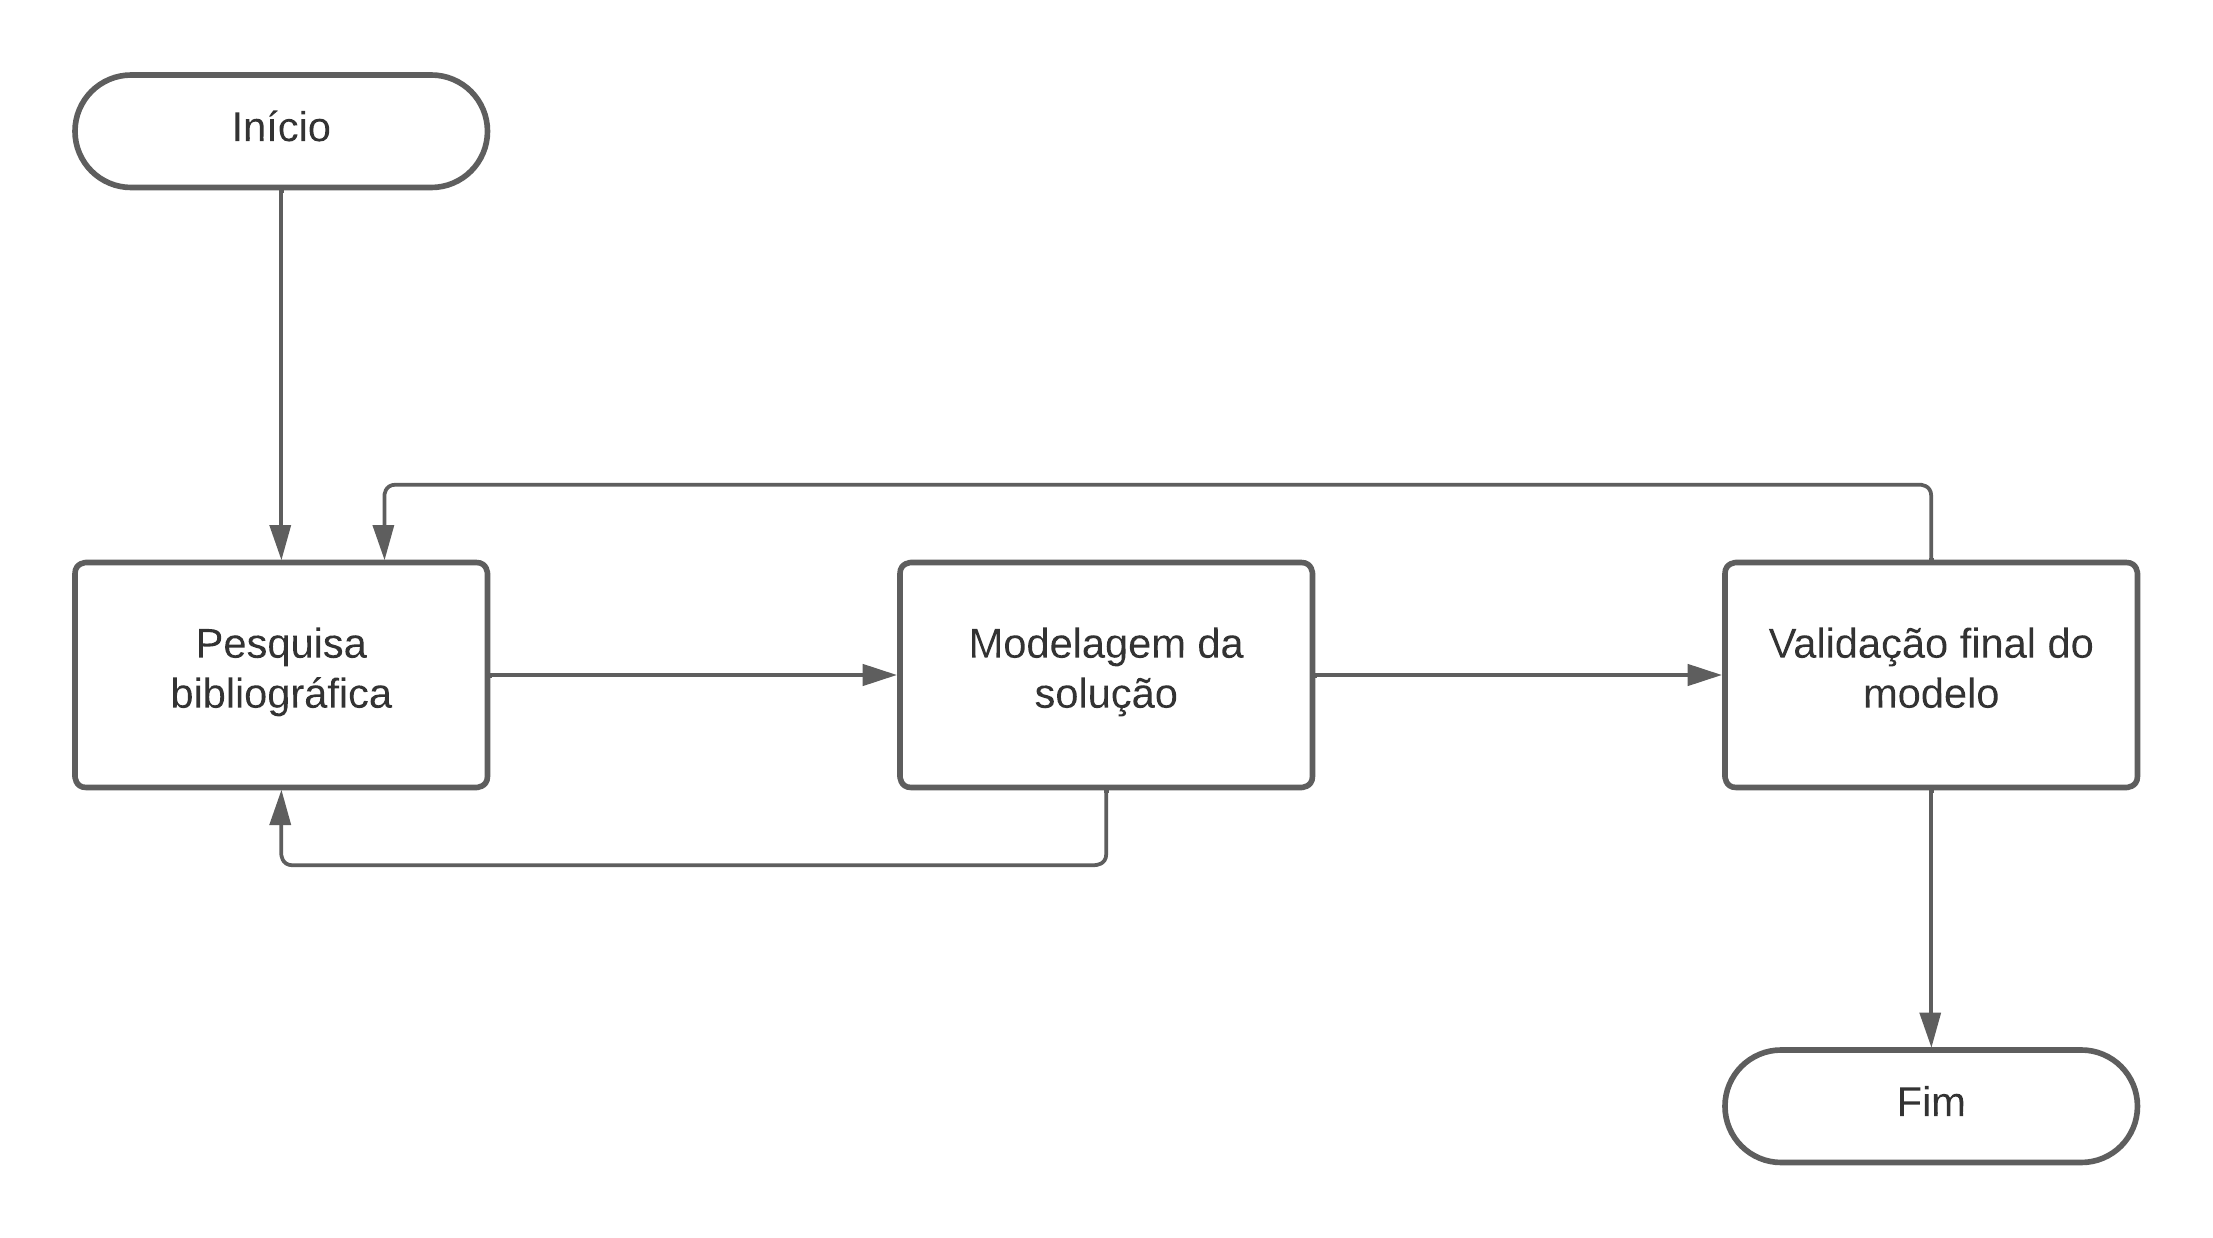
\includegraphics[scale=0.8]{fluxogramaMetodologia.png}
    \caption*{Fonte: Autora (2023).}
    \label{fig:fluxogramaMetodologia}
\end{figure}

A metodologia desempenhada no referente trabalho foi baseada na abordagem de \textit{Design Science Research} (DSR). Essa, por sua vez, é aplicada em pesquisas que almejam produzir um artefato (como um modelo ou uma aplicação) para solucionar um problema relevante \cite{dsrBook:2015}. A pesquisa deste trabalho cumpre as orientações para uma pesquisa de \textit{Design Science}, dispostas por \citet{dsrIS:2004}, reforçando como esta metodologia é apropriada para este trabalho. 

Assim, conforme os critérios da DSR, este trabalho visa produzir um artefato viável a partir do modelo a ser proposto para resolver o problema de desenvolvimento de robôs de serviço doméstico disposto anteriormente. Além de contribuir para a pesquisa de implementação de tecnologias para: a navegação autônoma e simulação robótica. Também, possui métodos específicos para a construção do modelo (seguindo a abordagem incremental de desenvolvimento de \textit{software}) e sua validação (utilizando casos de teste).

Para \citet{dsrBook:2015}, a metodologia DSR propõe uma pesquisa com 12 etapas, nas quais o problema a ser resolvido é identificado, as suas teorias e conceitos são estudados a partir de uma pesquisa bibliográfica e os artefatos semelhantes, para a solução do problema em questão, são constatados. Com isso, o artefato é desenvolvido e validado. Por fim, o resultado obtido é analisado e as conclusões são divulgadas para contribuir na área de pesquisa. Portanto, as três grandes etapas (Figura~\ref{fig:fluxogramaMetodologia}) a serem conduzidas neste trabalho se baseiam nesse fluxo de atividades proposto pelo DSR.

\section{Etapa de Pesquisa Bibliográfica}
A fim de desenvolver um robô autônomo móvel com as tecnologias mais adequadas e relevantes atualmente, foram realizadas duas pesquisas bibliográficas específicas. Essas pesquisas buscam identificar quais são as tecnologias mais utilizadas ao implementar a localização de um robô autônomo móvel, principalmente as abordagens utilizadas e os instrumentos de percepção do ambiente integrados.

Essas pesquisas bibliográficas específicas foram realizadas através do método de revisão da literatura narrativa com o uso de algumas características chaves da revisão sistemática. A fim de obter resultados mais imparciais e replicáveis, foram utilizados aspectos importantes da revisão sistemática dispostos em \citet{revisaoSistematica}, sendo eles: i) uma declaração explícita das perguntas a serem respondidas; ii) uma sequência de palavras-chave para cada pesquisa específica; iii) critérios de inclusão e exclusão para a filtragem dos artigos obtidos pelas buscas. 

Optou-se por realizar uma revisão narrativa por permitir uma compreensão do contexto de forma maleável \cite{revisaoNarrativa}. Visto que o objetivo das pesquisas bibliográficas mencionadas é compreender esse contexto geral dos temas supracitados para a tomada de decisão do uso das tecnologias mais relevantes e adequadas, foi identificado que a revisão sistemática não se encaixa. Isso se dá principalmente porque esse formato de revisão implica em uma análise detalhada de todos os dados obtidos em cada publicação acadêmica selecionada pela busca, além de requisitar uma sintetização dessas publicações, ou seja, informações desnecessárias para o alvo das pesquisas \cite{revisaoSistematica, literaturas}. Outro fator que impossibilita o uso da revisão sistemática é a exigência de pelo menos mais de um autor para tentar garantir o maior nível de imparcialidade possível \cite{revisaoSistematica, literaturas}.

Para encontrar os materiais acadêmicos relevantes foram utilizados os repositórios IEEE Xplore e ACM Digital Library, por serem específicos das áreas das Engenharias e da Computação. Além disso, foram definidas sequências de palavras-chave em inglês para buscar nos repositórios. Para focar a análise dos materiais, foram estabelecidos critérios de inclusão e exclusão para cada busca, filtrando os materiais com maior relevância para o assunto. 

Foi realizada uma sequência de pesquisas para identificar as tecnologias mais relevantes para localização do robô e percepção do ambiente. Primeiramente, foi efetuada a pesquisa para responder a pergunta: qual a abordagem mais utilizada para a localização de robôs autônomos móveis domésticos? Para isso, a busca foi realizada com a seguinte sequência de palavras-chave: 'autonomous mobile robot localization algorithms'. 

Com a resposta da pergunta inicial anterior, foi realizada a segunda pesquisa bibliográfica específica para responder outra pergunta: qual o instrumento mais utilizado para a percepção de um ambiente interno para um robô autônomo móvel que se localiza pela abordagem SLAM? Para essa segunda pesquisa, foi utilizada outra sequência de palavras-chave: 'slam sensing mobile robot'. Para ambas as buscas, foi utilizado o operador lógico AND entre cada palavra-chave, a fim de obter resultados mais específicos para os temas.

Em ambas as pesquisas bibliográficas específicas, foi realizada uma análise nos títulos e resumos dos artigos encontrados, para filtrar as publicações que não se encaixavam no escopo, seguindo as delimitações dos critérios de inclusão e exclusão, expostos na Tabela \ref{tab:prompts}. Os materiais foram filtrados com o apoio da plataforma Rayyan que disponibiliza uma estrutura para analisar artigos de uma forma mais eficiente \cite{rayyan}. 

\begin{table}[H]
\caption{Critérios de inclusão e exclusão}
\label{tab:prompts}
\resizebox{\textwidth}{!}{%
\begin{tabular}{p{7cm}|p{7cm}}
  \multicolumn{1}{c|}{\textbf{Inclusão}} &
  \multicolumn{1}{c}{\textbf{Exclusão}} \\ \hline
\begin{itemize}
    \item Aplicado em robótica móvel;
    \item Aplicado para ambiente interno doméstico;
    \item Escrito em inglês, espanhol ou português.
\end{itemize}&
\begin{itemize}
   \item Aplicado em navegação externa, água, aérea, indústria ou ambiente externo;
    \item Relacionado à realidade aumentada;
    \item Aplicado para veículos, drones, enxames de drones, múltiplo-robôs;
    \item Com necessidade de rede local, internet, wi-fi;
    \item Fora do escopo de robôs;
    \item Escrito em outro idioma que não seja inglês, espanhol ou português.
\end{itemize}% \\ \hline
\end{tabular}
%
}
\caption*{Fonte: Autora (2023).}
\end{table}

Dito isso, ambas pesquisas bibliográficas passaram por quatro momentos específicos, sendo eles:
\begin{itemize}
    \item Momento 1: Busca dos materiais acadêmicos nos repositórios com as palavras-chave definidas;
    \item Momento 2: Descarte dos materiais, resultantes da busca, que não pertencem ao período de 2018 a 2023;
    \item Momento 3: Descarte dos materiais, resultantes do momento anterior, que não são artigos publicados em periódicos;
    \item Momento 4: Descarte dos artigos, resultantes do momento anterior, que não cumprem os critérios de inclusão e/ou contém os critérios de exclusão.
\end{itemize}

Após a filtragem dos materiais encontrados na busca, foram identificados as tecnologias utilizadas em cada pesquisa, no intuito de encontrar qual delas é a predominante, e consequentemente, a mais relevante para os temas levantados.

\section{Etapa de Modelagem da Solução}
A modelagem foi realizada conforme os princípios da metodologia incremental de desenvolvimento de software. A abordagem incremental, de acordo com \citet{softwareSommerville:2011}, permite a implementação de funcionalidades essenciais em uma primeira versão e integrar outras funcionalidades a cada nova versão até que o sistema adequado seja desenvolvido conforme os requisitos levantados. 

Seguindo a metodologia incremental, em cada versão foram realizados o desenvolvimento e validação das novas funcionalidades. Esse ciclo de implementação tem o intuito de analisar se os requisitos levantados estão sendo alcançados corretamente, identificar falhas com antecedência e ajustar as funcionalidades antes de tornar o sistema mais complexo. 

\section{Etapa de Validação Final}
Com o modelo proposto completamente integrado, o mesmo foi conduzido por um processo de validação final de modo a analisar a adequação da proposta perante as especificações identificadas. Para isso, foram realizados testes de caixa preta conforme uma série de casos de testes definidos.

Os casos de teste são cenários que especificam uma entrada ou uma ação para os teste, além de um resultado esperado \cite{testes}. Para a validação do modelo proposto foram elaborados casos de teste baseados nos requisitos funcionais e não funcionais do robô e do ambiente simulados. O intuito dessa validação pelos casos de teste é identificar o comportamento do modelo proposto conforme as circunstâncias definidas previamente. Além disso, possibilita quantificar a adequação da solução proposta perante os requisitos identificados para o problema norteante da pesquisa. 

Os testes efetuados conforme os cenários especificados, utilizaram a técnica de testes de caixa preta, os quais visam verificar as funcionalidades específicas do sistema em alto nível \cite{testes}. Ademais, para os requisitos funcionais do robô, foi optado por realizar cinco repetições para cada caso de teste. Essas repetições têm o intuito de obter uma média de acertos perante os resultados esperados, visto que a execução do sistema pode encontrar instabilidades, mesmo sendo por simulação. Por fim, os resultados dos casos de teste foram classificados em 1) bem sucedidos, no qual o comportamento desejado foi obtido segundo a ação detalhada, e 2) não sucedido, caso o contrário. Os casos de teste com repetições foram considerados bem sucedidos se, e somente se, obtivessem uma porcentagem de sucesso maior que 50\%.

A fim de discernir as diferenças e similaridades entre o presente trabalho e as pesquisas correlatas que aplicam abordagens semelhantes para o desenvolvimento de um robô autônomo móvel, foi realizada uma análise comparativa. Essa análise consistiu em comparar os resultados,  expostos em trabalhos correlatos, sobre a implementação da navegação autônoma do robô móvel e do desenvolvimento em perspectiva geral.




\chapter{Fundamentação teórica}
\label{cap-revisao-bibliografica}

Um robô autônomo móvel capaz de executar tarefas rotineiras domésticas pode ser dividido em diversas funcionalidades individuais que contém suas próprias dificuldades e desafios. Dentre elas, uma pode ser considerada elementar e é o foco deste trabalho: a navegação do robô. Ademais, na área da robótica móvel, se encontram diversas abordagens para o controle lógico do robô, a sua estrutura física e até a forma de locomoção dele. Com isso, este capítulo expõe os conhecimentos básicos sobre estes tópicos e a simulação do modelo do robô a ser proposto.


\section{Robô Autônomo Móvel} %%MANTER
Os robôs autônomos móveis são sistemas mecânicos com certo grau de inteligência,  capazes de transitarem em um meio com liberdade, lidarem com as possíveis mudanças na sua trajetória e executarem tarefas determinadas \cite{practicalIndroductionNehmzow:2012}. 

Os robôs autônomos móveis são constituídos por uma estrutura física, seu corpo, composta por elementos que possibilitam a sua percepção do meio que estão inseridos (sendo estes os sensores) e que executam ações diante do mesmo (denominados como atuadores) \cite{mobileRoboticsJaulin:2019}.
Para controlarem seu corpo, é implementado um sistema de controle inteligente que toma decisões a partir da interpretação dos dados coletados pelos sensores e essas decisões são enviadas aos atuadores para que a atividade em execução prossiga \cite{mobileRoboticsJaulin:2019}. 

Esses equipamentos são utilizados em diversas áreas, como medicina, agricultura e militarismo \cite{mobileRoboticsJaulin:2019}. 
Através deles, é possível executar tarefas comumente realizadas por algum ser vivo (como seres humanos ou animais) ou veículos, tais quais podem ser perigosas ou não desejáveis por uma determinada razão \cite{mathematicsModelsKelly:2013}.
Por poderem ser estruturas robustas,  permitem chegar a localizações que os seres humanos não conseguem acessar \cite{mobileRoboticsJaulin:2019}. 
Isso permite a execução de funcionalidades como: transportação, inspeção e segurança\cite{mobileRoboticsJaulin:2019}. 

Assim, os robôs móveis autônomos são vantajosos principalmente por definirem, praticarem e adaptarem um planejamento da execução de uma tarefa conforme o seu aprendizado do ambiente \cite{practicalIndroductionNehmzow:2012}. 
O diferencial entre os robôs móveis autônomos e outros robôs dependentes, é a sua adaptabilidade perante mudanças no ambiente e não conterem ações pré-definidas \cite{practicalIndroductionNehmzow:2012}.

Sendo assim, um dos maiores desafios encontrados na área é o tratamento e tomada de decisões do robô perante mudanças constantes em um ambiente interno com um alto grau de incerteza, como pessoas (sejam elas adultas, crianças ou idosos) e animais transitando, ademais do próprio  posicionamento de móveis e objetos \cite{practicalIndroductionNehmzow:2012}. 
 
Dito isso, esta seção apresenta os conceitos básicos de navegação, da estrutura física de um robô móvel autônomo e a discussão sobre as abordagens de arquiteturas mais relevantes para o seu controle lógico.


\subsection{Navegação Autônoma do Robô } %%INCREMENTAR

A navegação de um robô de forma independente não constitui apenas do dispositivo vagar pelo local aonde se encontra. Em primeiro lugar, é necessário que ele entenda onde está e com isso possa identificar o seu ponto geográfico no espaço em que atua. Em conjunto com a tarefa que deseja executar e as informações do ambiente, o robô inicia o processo de planejamento da trajetória que precisa percorrer até o seu destino. Por fim, a partir das decisões tomadas para seguir uma rota, ele se moverá inteligentemente até o destino, evitando os obstáculos e lidando com possíveis mudanças no meio. Assim, podemos afirmar que a navegação autônoma do robô é composta por quatro tarefas primordiais: i) percepção do ambiente, ii) localização, iii) planejamento, iv) locomoção \cite{mobileRobotsSiegwart:2011}. 

É necessário que o papel do robô e o seu ambiente de atuação sejam bem definidos. Desse modo, as funcionalidades essenciais afirmadas conseguem ser integradas, a fim de atender melhor os requisitos e manter a confiabilidade no dispositivo \cite{mobileRobotsSiegwart:2011}. 
Isso é notório ao comparar o funcionamento de um robô com um braço robótico que empilha paletes em uma fábrica em detrimento a um robô aspirador de pó — apesar de ambos serem robôs autônomos móveis.

Como explicitado, a primeira ação que um robô autônomo móvel deve executar antes de se mover por um ambiente, é a percepção do mesmo. Entender qual a situação atual do meio e as suas características, pode ser realizado por um conjunto de sensores que coletam dados ao redor do robô, como luminosidade, amplitude do som e medida da distância \cite{mobileRobotsSiegwart:2011}. 
Com o conhecimento adquirido através das informações processadas com os dados reunidos pelos sensores, é possível identificar o ponto geográfico onde o robô se encontra no espaço \cite{mobileRobotsSiegwart:2011}.

Com a percepção completa do ambiente, as informações registradas são utilizadas para localizar o robô no espaço. \citet{mobileRoboticsJaulin:2019} reconhece a localização como a identificação da posição do robô no ambiente e seu grau de liberdade para movimentação. Essa etapa é considerada um dos principais desafios da navegação, existindo diversas abordagens.

Entre as abordagens existentes para a localização, é mais comum o uso de modelos reais (como mapas topográficos), podendo ser criados dinamicamente enquanto o robô navega pelo ambiente ou ser uma entrada pré-definida do sistema \cite{mobileRobotsSiegwart:2011}. 
Por outro lado, esse método é questionado, pois, muitas vezes, o modelo não é verossímil à realidade. Para isso, são utilizadas técnicas alternativas como equações de matemática com ângulos e características cinemáticas de marcos ao redor do robô \cite{mobileRoboticsJaulin:2019}.

A localização do robô em um meio e o mapeamento desse ambiente é um problema bem conhecido na área da robótica móvel \cite{SLAMProblem:1991}. Uma das alternativas encontradas para ultrapassar essa questão são os algoritmos que implementam a abordagem SLAM (em inglês \textit{Simultaneous Localization and Mapping}). A abordagem de Mapeamento e Localização Simultânea tem o intuito de produzir um mapa consistente do ambiente, a partir de leituras de sensores ou câmeras, e obter a localização estimada do robô conforme os pontos reais encontrados no meio e os seus correspondentes no mapa criado \cite{SLAMDefinitionEvolution:2021, SLAMTutorialII:2006, SLAMReview:2015}. Uma das maiores vantagens encontradas na utilização do SLAM é a irrelevância da localização do robô e das informações do ambiente antes da sua execução \cite{SLAMReview:2015}.

Após compreender o ambiente e onde o robô se encontra, esse elabora um plano para seguir sua trajetória a fim de terminar a tarefa em execução.
Nesse contexto, surge outro problema significativo da navegação: a capacidade de chegar ao seu destino de forma eficiente e confiável \cite{mobileRobotsSiegwart:2011}.

Como apontam \citet{mobileRobotsSiegwart:2011}, um ponto crítico da tarefa de planejamento é a própria movimentação do robô. A cada “passo” que ele avança, as características do ambiente mudam, como, por exemplo, o robô pode estar chegando cada vez mais perto de uma parede que deve desviar em um futuro próximo. Dessa forma, o robô também atua no meio, intervindo nas suas características. 

Especificamente, ao tratar de um robô autônomo móvel que atua em um ambiente interno como um domicílio, a dificuldade aumenta, por ser um espaço dinâmico e vivenciado por seres humanos que são menos previsíveis do que objetos ou móveis parados. Portanto, é fundamental que a arquitetura do robô tenha um nível de inteligência suficiente para elaborar um caminho, evitando colisões, e o seu redirecionamento para longe dos obstáculos e mais próximo do destino.

Embora um planejamento sólido para navegação, considerando os aspectos de percepção e localização, seja de fundamental importância, a estratégia de locomoção adequada não pode ser deixada de lado. Segundo \citet{mobileRobotsSiegwart:2011}, existem duas principais maneiras de um robô se mover pelo espaço: uma forma veicular (por rodas) ou assemelhando-se a biologia (por pernas). 

O uso de rodas é comumente optado para robôs que atuam em terrenos mais regulares e lisos, visando um melhor desempenho. Neste contexto, a escolha da roda usada impacta a direcionalidade do robô. De um lado, há a roda comum (Figura~\ref{fig:rodas}(a)) que traz a necessidade de mudar o eixo do corpo para se locomover em outra direção e de outro, há rodas como a roda Mecanum (Figura~\ref{fig:rodas}(b)) que permite a mudança de direção sem a mudança no eixo. Além do seu design, a quantidade de rodas e a disposição delas impactam na estabilidade, controle e manobras do robô. 
 
\begin{figure}[h]
    \centering
    \caption{Diferença entre roda padrão e roda Mecanum}
    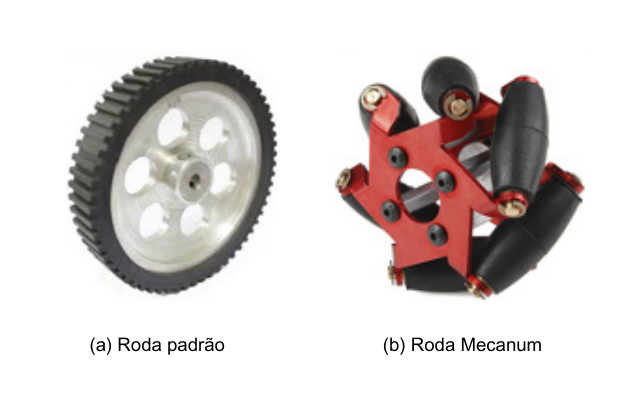
\includegraphics[scale=0.5]{rodas.png}
    \caption*{Fonte: \citet{wheels:2018}.}
    \label{fig:rodas}
\end{figure}

\subsection{Abordagens de Arquitetura de Controle} %%ATUALIZADO

A navegação consegue ser bem sucedida apenas quando os seus quatro aspectos fundamentais (percepção, localização, planejamento e locomoção) são controlados corretamente de forma uníssona por uma arquitetura inteligente \cite{mobileRobotsSiegwart:2011}. Para isso, existem duas abordagens principais que possam ser utilizadas: a inteligência artificial (IA) clássica e a arquitetura de subsunção.

Conforme explicado em \citet{practicalIndroductionNehmzow:2012}, a IA clássica se constitui em um ciclo repetitivo de coletar informações do ambiente por sensores, as quais alimentam uma sequência de módulos dependentes que realizam o seu processamento e geram uma ação para os atuadores do robô. Os dados coletados do espaço onde o sistema está inserido é transmitido diretamente para o primeiro módulo de processamento e os próximos módulos utilizam as informações dos seus anteriores para criar e atualizar ou comparar com um modelo do mundo real. 

Para \citet{practicalIndroductionNehmzow:2012}, entre as principais desvantagens da abordagem clássica  se tem o uso único do modelo do mundo, pelos módulos de processamento, ao invés das informações em tempo-real coletadas pelos sensores. Outra questão crítica é a dependência alta entre cada módulo, permitindo a falha do sistema completo caso algum módulo encontre um erro. Por fim, também existe a preocupação que esta abordagem não se adeque à necessidade do robô de ter reações rápidas.

Perante projetos com a necessidade de utilizar uma abordagem que não dependesse de representações simbólicas, com menor custo computacional e com maior conexão entre as informações reais do ambiente e as decisões tomadas, é eficiente aplicar um conceito alternativo ao de IA clássica, como a  arquitetura de subsunção de Rodney Brooks.

A arquitetura de subsunção proposta em \citet{brooks85} constitui camadas que representam atividades comportamentais independentes. Sua principal diferença em relação à abordagem clássica é a estrutura paralela da arquitetura. Esse paralelismo é dado através dos módulos (processadores) que recebem dados dos sensores, comunicam entre si assincronamente e executam ações nos atuadores em conjunto, podendo ser visualizados como camadas na horizontal em detrimento de uma execução mais vertical como na IA clássica (Figura~\ref{fig:abordagens}). 

\begin{figure}[h]
    \centering
    \caption{Diferença entre a arquitetura de subsunção e IA clássica}
    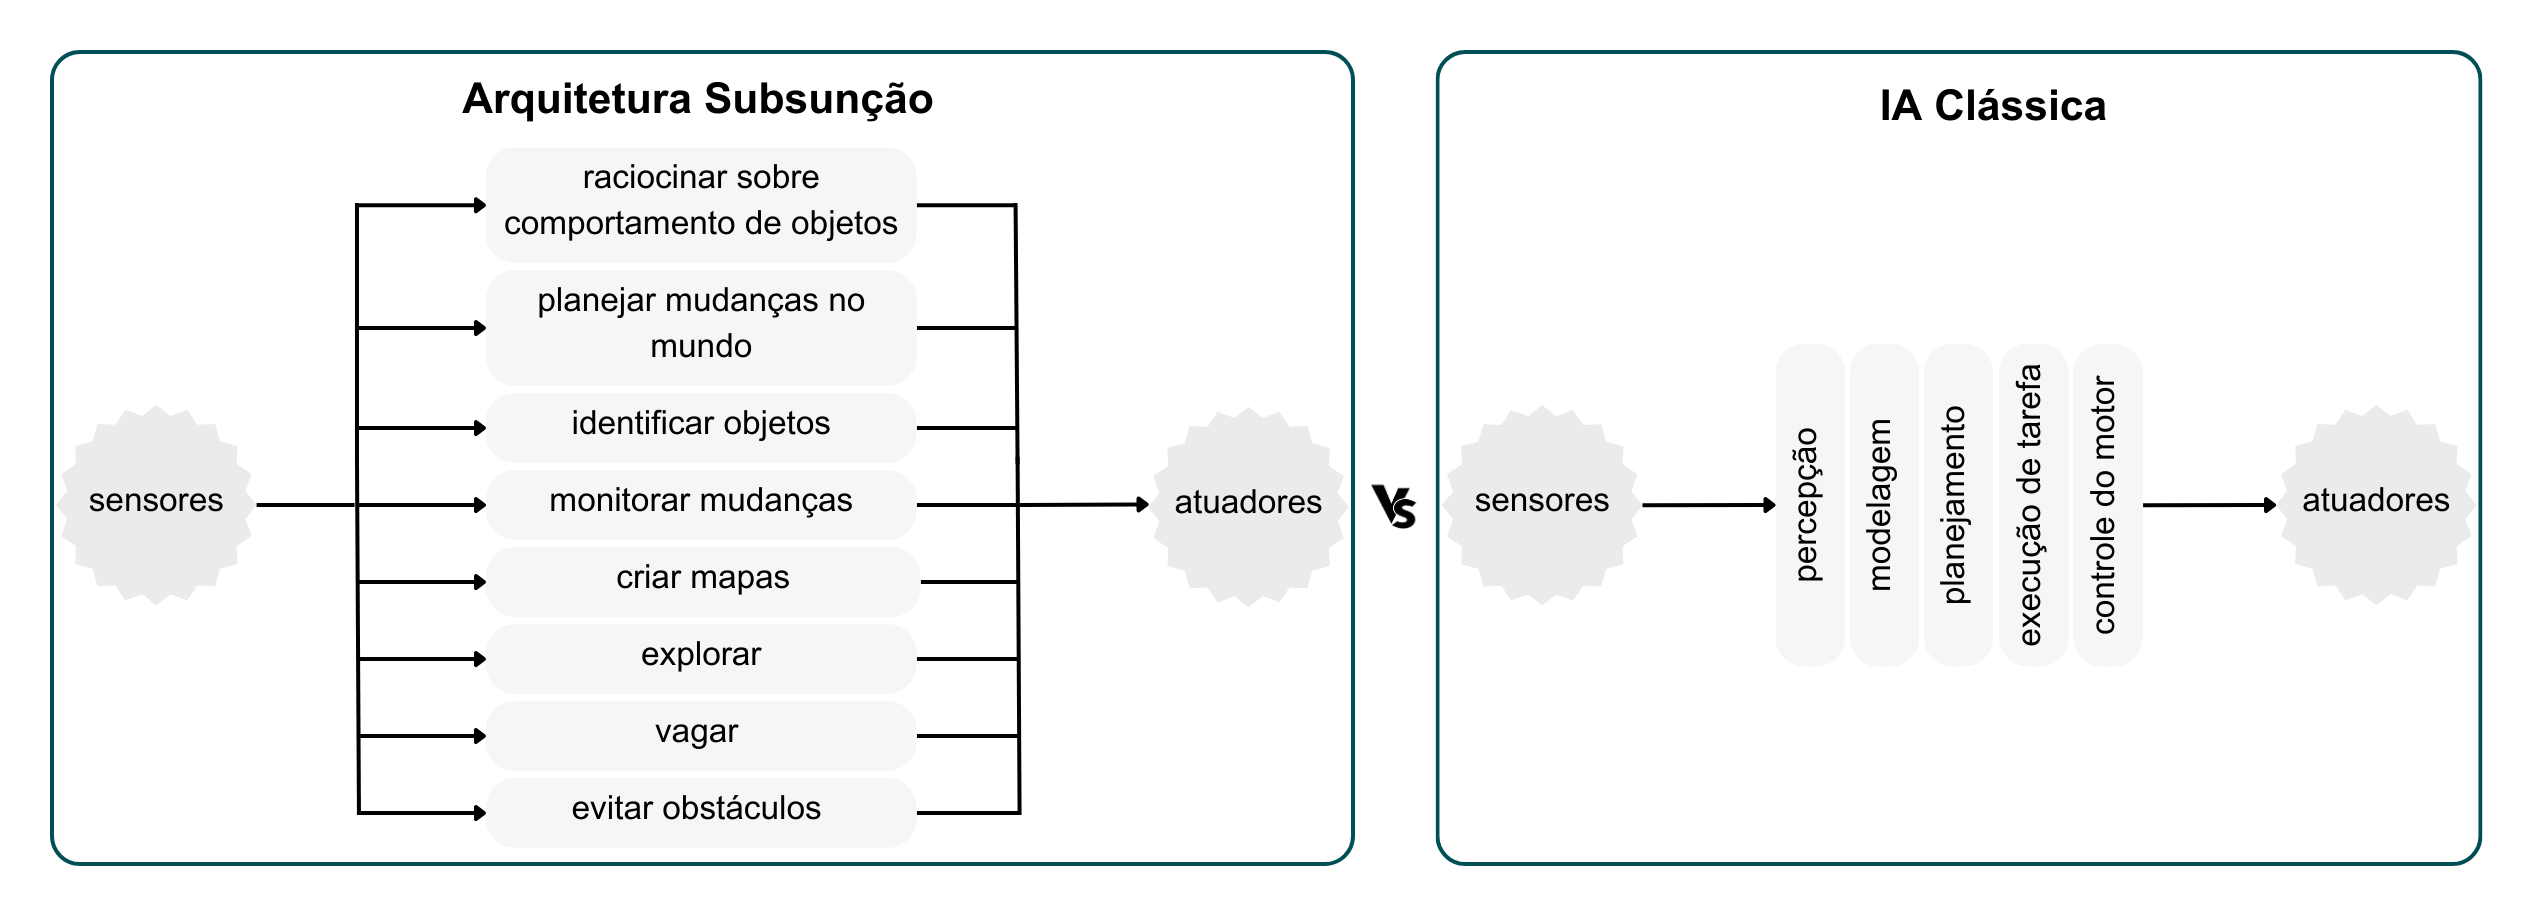
\includegraphics[scale=0.2]{abordagens.png}
    \caption*{Fonte: Adaptação de \citet{brooks85} pela autora.}
    \label{fig:abordagens}
\end{figure}

As camadas da arquitetura de subsunção foram projetadas por \citet{brooks85} como níveis de competência que especificam, informalmente, uma classe de comportamentos desejáveis. Neste trabalho, Brooks utilizou cinco níveis que contemplam navegação, com e sem rumo, evitando colisões, exploração e mapeamento do ambiente,  planejamento de rotas e tratamento de mudanças no espaço. 

\citet{brooks85} expõe nove paradigmas para os sistemas baseados na arquitetura proposta. Entre eles, salienta-se a importância da simplicidade em diversos aspectos, como o próprio sistema de controle a ser implementado e a comunicação entre as camadas. 

Outra questão levantada na arquitetura de subsunção é o uso de modelos do mundo (tais quais não são usados unicamente durante o processamento, pois todos os módulos têm acesso às informações coletadas pelos sensores). Eles visam uma melhor verossimilidade a realidade a partir do uso de mapas não relacionais de três dimensões e não artificiais. Por fim, também é ressaltado a necessidade da durabilidade e robustez do sistema sem a interferência de humanos.


\subsection{Estrutura Física do Robô} %%ATUALIZADO

A estrutura física do robô precisa refletir e acomodar o ambiente em que atua para as suas tarefas serem executadas correta e eficientemente. O corpo, que engloba o sistema implementado, pode consistir em sensores que irão coletar dados do ambiente e da condição do próprio dispositivo, atuadores para terem ações sobre o meio, partes mecânicas como braços robóticos para manipulações e elementos para o processamento geral e individual dos outros componentes.

A percepção do ambiente e a execução das tarefas pelo robô dependem significativamente dos transdutores para tais fins, disponibilizados no seu corpo. Como \citet{instrumentacao:2013} explica, os transdutores são dispositivos utilizados para captarem dados (grandezas físicas)  do ambiente e transformarem em informações (sinais elétricos) para o sistema processar ou transformarem decisões tomadas (sinais elétricos) pelo processamento do sistema em ações (grandezas físicas) executadas no ambiente. Assim, existem dois tipos de transdutores: os sensores e os atuadores. 

Os sensores são responsáveis em permitir que o robô compreenda o ambiente que está inserido através das grandezas físicas coletadas (entradas) e transformadas em sinais elétricos que então são processados em uma informação útil (saída). Apesar de comumente os sensores obterem entradas que não são as em foco (entradas espúrias), são utilizados diversos mecanismos de filtrar entradas e calibrar estes instrumentos para seu melhor desempenho. 

O mundo dos sensores  é versátil e variado, dentre os existentes para a percepção de objetos se tem o sensor LiDaR (\textit{Light Detection and Ranging}), o qual emite uma onda ótica e captura o tempo para que o reflexo desse feixe de luz retorne \cite{lidarComparative:2021, lidarProgress:2022}. Seu objetivo principal é descobrir a distância entre o corpo que está embutido e os objetos à sua frente \cite{lidarProgress:2022, lidarComparative:2021}. Esse sensor é utilizado em diversas situações, como veículos autônomos, equipamentos médicos precisos e monitoramento, podendo ser mais preciso do que sensores que utilizam ondas sonoras \cite{lidarProgress:2022, lidarDetection:2019}.

Os atuadores, por sua vez, possibilitam que as tarefas planejadas pelo sistema se concretizem a partir do inferimento de grandezas físicas em elementos mecânicos presentes no corpo do robô. Este comportamento pode ser visualizado quando o controle lógico de um robô móvel autônomo decide se virar para direita e pelos atuadores, os motores necessários são acionados para realizar a rotação das rodas.  

A arquitetura de subsunção apresentada por \citet{brooks85} também trata sobre questões do corpo físico do robô. Em primeiro lugar é retratado que o dispositivo deve possuir uma estrutura que o permite trafegar em espaços de convivência de humanos, isso implica que ele deve ter uma certa altura para conseguir enxergar objetos em cima de móveis, por exemplo, e uma largura máxima para conseguir passar por portas e corredores. 

Em \citet{brooks85}, também é reforçada a importância da independência dos sensores e outros instrumentos de percepção, trazendo maior robustez ao sistema e confiabilidade, mesmo se alguns de seus sensores apresentarem erro. 

\section{Simulação} %%ATUALIZADO

A construção de um robô e o teste da sua estrutura em conjunto com o software de controle requerem um leque grande de recursos e bastante tempo disponível. Por isso, quando há uma escassez, limitações ou nenhuma disponibilidade de algum desses requisitos, podem ser usados simuladores que representam e interpretam o mundo real virtualmente. 
Tais ferramentas são utilizadas em diversos campos das engenharias, inclusive a robótica, sendo muito prático para pesquisa e educação \cite{usarsimCarpin:2007}. 

Como o intuito dos experimentos virtuais consiste em simular eventos reais que poderiam existir em testes no mundo tangível, é preciso ter cautela e incluir a maior veracidade possível ao ambiente e robô simulados \cite{aprendizadoHeinen:2010}.  
Assim, se faz necessário a modelagem de leis da física presentes no universo real e a interação com ambiente por sensores e atuadores, para o robô sofrer quedas e colisões segundo a situação, conforme a realidade \cite{usarsimCarpin:2007, evolucaoHeinen:2006}.  

A maior preocupação acerca do uso da simulação é a sua capacidade de conter detalhes verídicos e ser o menos limitante possível, visto que o mundo  real é muito mais complexo  \cite{wanderingMiglino:1994}. 
Com um experimento por \citet{wanderingMiglino:1994} para o teste de algoritmos que propõem a evolução de robôs vagantes, foi demonstrado que a simulação e a execução real desses robôs conseguem ser bem similares, obtendo melhor desempenho em robôs tangíveis para alguns casos.

Os simuladores permitem interpretar situações reais de forma virtual. Entretanto, é necessário intermediar os elementos (sensores e atuadores) do robô com seu controle lógico. Isso é possível ao implementar ROS (Sistema Operacional de Robô), o kit de desenvolvimento para aplicações robóticas \cite{ROS} Uma das maiores vantagens do ROS é a sua coleção de bibliotecas e módulos para utilizar em diversas ocasiões robóticas, sem a necessidade de desenvolver algoritmos do início \cite{ROS}. Além disso, ROS é multi-plataforma, possibilitando o desenvolvimento único  para a simulação e a realidade \cite{ROS}.

Nesse contexto de programas de simulação robótica,  é possível encontrar desde ambientes gratuitos mais rústicos para pesquisa e educação, como USARSim,  até os mais profissionais oferecidos por empresas especializadas em desenvolvimento de eletrônicos, como a Nvidia que oferece o Nvidia Omniverse e a biblioteca IsaacSim para simulação de robótica. 

Também é possível encontrar soluções no meio-termo que são muito utilizadas como WeBot da Cyberbotics, Gazebo e CoppeliaSim, tais quais são \textit{open source} e utilizam a biblioteca Open Dynamics Engine (ODE) para trazer aspectos da física na simulação.  A ODE também pode ser integrada em plataformas de criação de jogos, como a Unity, transformando-as em ambientes simuladores de robótica. 

Dentre os supracitados, pode ser destacado o simulador \textit{open-source} Gazebo \cite{gazeboDesigns:2004}. Algumas de suas características que o faz ser ressaltado em meio aos diversos outros simuladores são: i) modelos de robôs e ambientes prontos; ii) comunidade ativa que visa incrementar novos modelos de robôs e ambientes; iii) integração com ROS \cite{gazeboDesigns:2004, pickSimulatorFarley:2022}.

\section{Considerações Adicionais da Fundamentação Teórica}

Este capítulo permitiu uma fundamentação teórica nos principais tópicos dos robôs autônomos móveis e a simulação robótica. Foram discutidos os quatro aspectos da navegação autônoma de um robô que consiste na percepção do ambiente, sua localização, o planejamento de uma rota a ser seguida e a sua locomoção. 

Além disso, foi compreendida a arquitetura de subsunção para o controle do robô e a sua vantagem com relação à abordagem tradicional da inteligência artificial. Ainda no contexto dos robôs, foram introduzidas as necessidades para a sua estrutura física.  Por fim, foi explorado o tema de simulação robótica, alguns programas simuladores reconhecidos e o sistema operacional de robô. 

Com essa compreensão do funcionamento de robôs autônomos móveis e da simulação robótica, se torna possível analisar mais vigorosamente trabalhos que almejam desenvolver um robô com a capacidade de navegar de forma autônoma em um ambiente interno desconhecido. Assim, o próximo capítulo expõe variados trabalhos correlatos, além das suas diferenças e similaridades com o AtmosBot.




\chapter{Trabalhos Correlatos}
\label{cap-trabalhos-relacionados}
Este capítulo expõe variadas pesquisas realizadas anteriormente que se assemelham ao presente trabalho e seus principais aspectos.

\section{Robô de Serviço Doméstico Herbert}
Em primeiro lugar, a partir da definição da arquitetura de subsunção e com a orientação do seu criador, Rodney Brooks, \citet{herbert:1988} realizou um experimento para amostrar os princípios dessa arquitetura através da implementação do robô autônomo móvel Herbert.  

O projeto \citet{herbert:1988}  expõe um robô completamente autônomo utilizado em ambientes internos como uma casa, capaz de realizar tarefas de navegação, reconhecimento e manipulação. A sua estrutura física (Figura~\ref{fig:herbert})  é composta por uma base pronta adquirida com o foco na direção do robô, bem como uma parte superior que contém equipamentos de processamento e um braço robótico. 

\begin{figure}[H]
    \centering
    \caption{Estrutura física do Robô Herbert}
    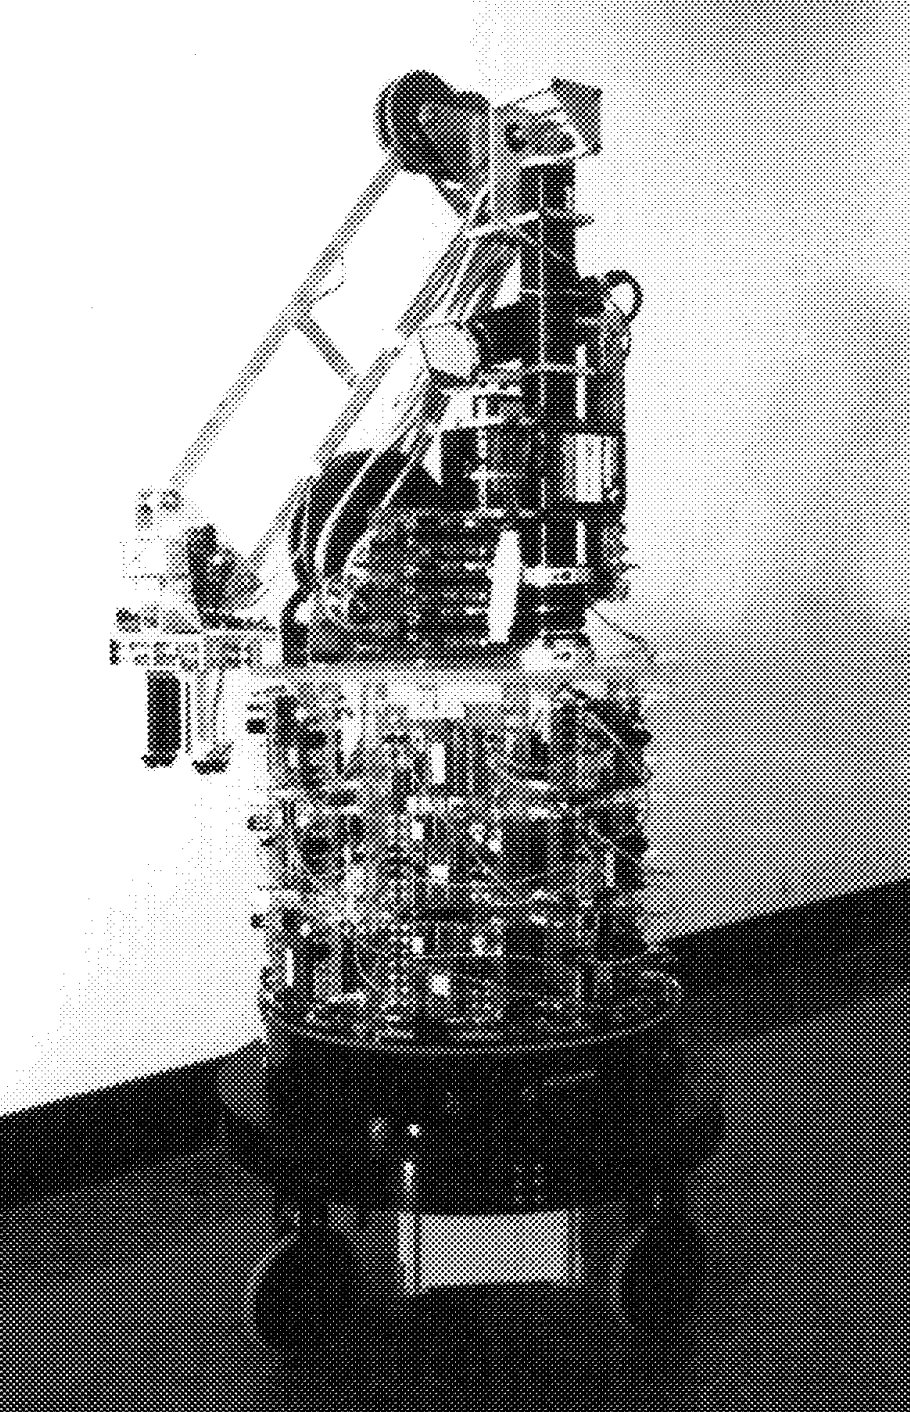
\includegraphics[scale=0.2]{herbert.png}
    \caption*{Fonte: \citet{herbert:1988}.}
    \label{fig:herbert}
\end{figure}

A base do robô Herbert contém a alimentação de energia própria e um computador servo para realizar o mecanismo de direção, o qual atua em um único motor e três rodas. A parte superior do robô é composta por um braço robótico leve e com grau de liberdade suficiente para pegar e soltar objetos no nível do chão e de uma mesa. Essa parte também contém um sensor infravermelho para o robô conseguir se esquivar de obstáculos próximos, fixos ou em movimento, e um sensor scanner de alcance a laser para reconhecimento de objetos. 

Para o controle lógico do robô através da arquitetura de subsunção, foram utilizadas placas com microprocessadores CMOS de 8 bits  que compartilham entre si apenas energia. Para integrar o reconhecimento lógico de objetos com o scanner, foi combinado com o sensor uma árvore de processadores de visão orientada por linha. 

O robô Herbert conseguiu ter um consumo energético baixo para a sua época por ser estruturado por componentes CMOS, além de ter uma resposta mais rápida aos obstáculos por conta do sensor infravermelho que possibilita uma varredura do ambiente em 360 graus. Ademais, sua estrutura foi arranjada de uma maneira que todos seus subsistemas - como as placas de circuitos -  conseguem ser removidas, ajustadas e devolvidas ao corpo do robô com fácil acesso. 

Por ser um projeto realizado no fim dos anos 80, os equipamentos utilizados e as capacidades do robô são limitantes. Apesar de utilizarem processadores com menor custo energético, o dispositivo consegue transitar e realizar suas tarefas pelo ambiente por apenas uma hora. 

Outra desvantagem reconhecida no trabalho é a capacidade do sensor infravermelho em reconhecer a distância de certos objetos conforme o seu tamanho, localização no plano e cor, ou seja, objetos escuros são mais difíceis de serem compreendidos pelo sensor e o mesmo pode se confundir com a profundidade de um objeto pequeno mais próximo e um grande mais longe. Por fim, para realizar todas as tarefas, ao navegar pelo ambiente, o agente armazena as informações de distância e ângulos viajados para conseguir retornar a sua origem depois de cada objeto apanhado para descartá-lo.

\section{Robô de Serviço Doméstico Justina}
Os robôs autônomos de serviço continuaram a ser pesquisados e projetados durante os anos, obtendo avanços notáveis. Similarmente ao robô Herbert, em 2019, foi criado o robô Justina, por \citet{justina:2019}. Este robô emergiu por meio das competições robóticas, conquistando o primeiro lugar no RoboCup@Home de 2019, mostrando o quão crucial essas competições são para o desenvolvimento das tecnologias e motivação da pesquisa na área de robótica, inclusive no tema de robôs de serviço doméstico. 

O equipamento foi produzido pela equipe Pumas, composta por pesquisadores da Universidade de Autonomia Nacional do México. Apesar do time participar constantemente das competições há mais de uma década, sempre buscou aprimorar as tecnologias e conceitos implementados nos seus robôs. Para o RoboCup@Home, mostrou como diferencial um sistema com maior capacidade de compreender a linguagem natural dos comandos de voz dados pelos seres humanos e de manipular objetos com superfícies com menos texturas e geometria mais plana.

O robô Justina (Figura~\ref{fig:justina}) compõe em sua estrutura física uma base com duas rodas onidirecionais, seguida por um torso móvel  metálico capaz de se elevar, dois braços robóticos para a manipulação dos objetos e uma parte superior com suporte do tipo \textit{pan and tilt}. Neste suporte, foi fixado um Kinect da Microsoft e logo acima, um microfone direcional (utilizado para receber os comandos de voz). 

\begin{figure}[H]
    \centering
    \caption{Estrutura física do Robô Justina}
    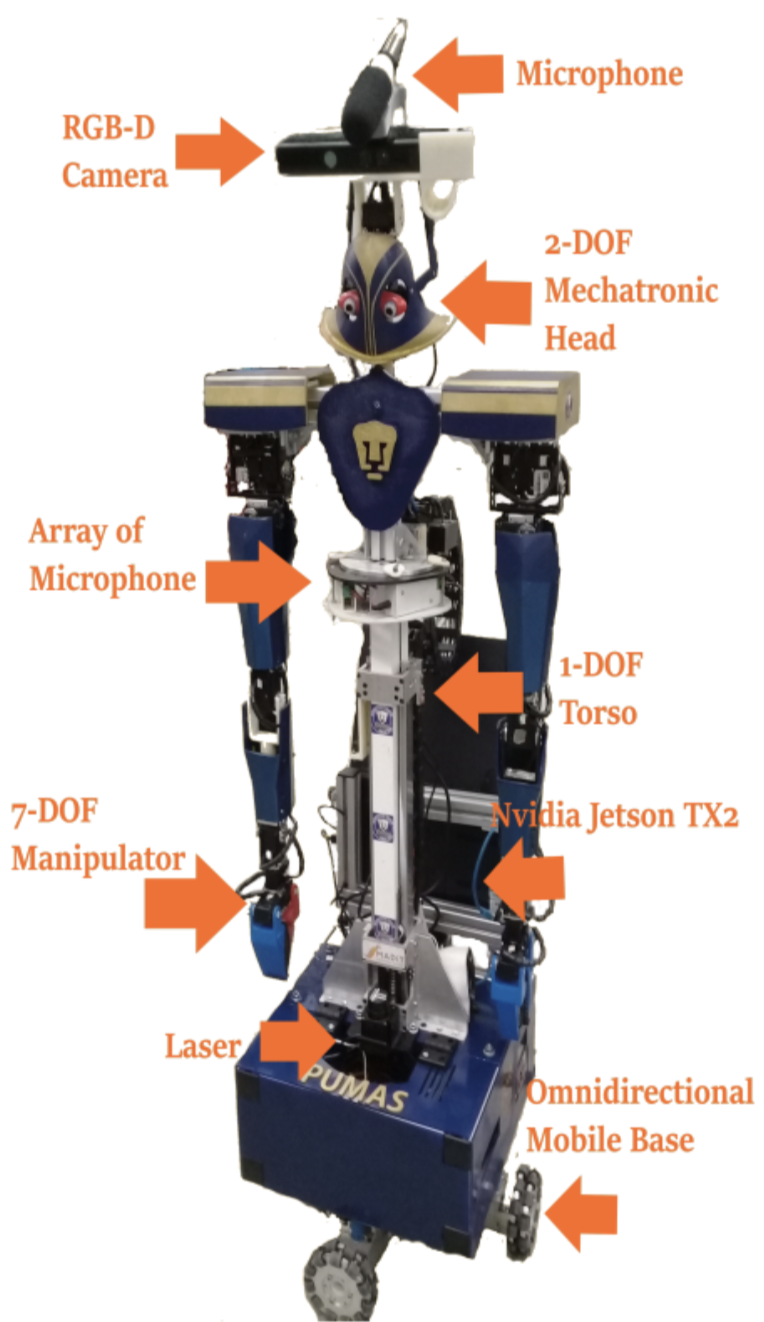
\includegraphics[scale=0.4]{justina.png}
    \caption*{Fonte:\citet{justina:2019}.}
    \label{fig:justina}
\end{figure}

Além da câmera RGB-D do Kinect, são utilizados uma segunda câmera RGB, um laser e quatro microfones para perceber o ambiente onde o robô está inserido. Além disso, como retorno para os seres humanos, foram instaladas caixas de som que emitem uma voz sintetizada informando dados da tarefa em execução. Por fim, para realizar o processamento de imagem obtida a partir das câmeras, foi utilizado um sistema embarcado da NVidia.


O robô da equipe Pumas baseia-se na arquitetura VIRBOT, própria para robôs de serviço domésticos, implementada mediante um conjunto de módulos independentes que executam tarefas próprias e se comunicam entre si. Essa comunicação entre os componentes é realizada pelo sistema operacional de robô (ROS). 

O sistema VIRBOT é composto por quatro camadas nas quais ocorre o processamento das informações externas e internas do robô,  planejamento de objetivos ativados a partir dessas informações, localização do corpo no ambiente por mapas criados pela técnica SLAM e, por fim, a execução das ações e movimentos planejados. De acordo com \citet{justina:2019}, a próxima funcionalidade a ser aprimorada seria deslocamento em todas as direções para melhorar o desempenho da navegação.

\section{TurtleBot3 com SLAM}
No contexto apenas da navegação autônoma, muitas abordagens podem ser utilizadas para resolver o mesmo problema: fazer com que o robô planeje e percorra uma trajetória em um ambiente sem a interferência de humanos. Em \citet{navegacaoSlam:2022} é exposto o uso de SLAM como método eficaz para uma navegação autônoma pelo seu robô Turtlebot3 Burger (Figura~\ref{fig:turtlebotSLAM}). 

\begin{figure}[H]
    \centering
    \caption{Estrutura física do TurtleBot3}
    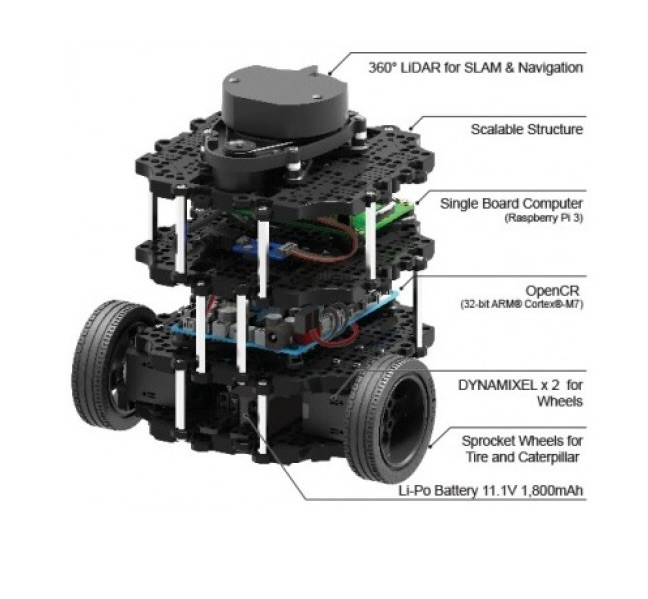
\includegraphics[scale=0.35]{turtlebot3.jpeg}
    \caption*{Fonte:\citet{turtleBot3Burger:2021}.}
    \label{fig:turtlebotSLAM}
\end{figure}

As informações do ambiente foram capturadas por um sensor LiDaR e utilizadas, em conjunto com a odometria  (informação de deslocamento a partir das revoluções das rodas) do robô, no processo SLAM. A fim de melhorar a experiência com a abordagem SLAM, foi utilizado o algoritmo AMCL (\textit{Adaptive Monte Carlo Localization}), sendo uma a versão aprimorada do algoritmo original Localização Monte Carlo. Além disso, o ROS é utilizado como o intermediador entre o sistema, os sensores e o controle lógico (no qual é executado o SLAM adaptado) do Turtlebot3 Burger. 

Visando testar facilmente a solução proposta em comparação com o mapeamento e navegação comum, foi usado o simulador Gazebo. Entretanto, os dois métodos foram testados no mundo real também para assegurar resultados condizentes com a realidade. Com esses experimentos foi apontado que o uso do SLAM aperfeiçoado com o algoritmo de Localização Adaptativa de Monte Carlo tornou a navegação mais resiliente e com maior acurácia.


\section{Robô Autônomo Móvel DPoom}

O desenvolvimento de um robô autônomo móvel, em muitos casos, pode incluir a implementação de recursos que tornam o robô mais custoso, em questão de processamento e preço. Em \citet{dpoom}, seu principal objetivo é diminuir o custo computacional e monetário dos robôs autônomos móveis. Para reduzir o valor da estrutura física do robô, foi utilizada uma câmera RGB-D (capaz de capturar a profundidade dos itens, além da imagem comum colorida) para a percepção do ambiente, ao invés do sensor LiDaR, comumente utilizado e com maior custo. 

Além disso, foi adicionada uma adaptação, menos custosa computacionalmente, do algoritmo clássico de aprendizado por reforço profundo, para evitar obstáculos ao longo da locomoção do seu robô DPoom. Em conjunto, \citet{dpoom} implementou a criação de mapas e posicionamento em tempo real com algoritmo de SLAM integrado a câmera RBG-D. Com isso, foi possível retirar a necessidade da utilização de uma GPU (\textit{Graphic Processing Unit}) e manter o desempenho ideal em tempo real, usufruindo apenas de uma placa-mãe de baixo custo.

A fim de validar seu sistema desenvolvido, \citet{dpoom} integrou todas as funcionalidades com ROS e testou, primeiramente, no simulador Gazebo com uma variação de dez ambientes domésticos estáticos e dinâmicos. O  DPoom (Figura~\ref{fig:dpoom}) também foi testado em ambientes internos reais, com humanos se movimentando ao longo do meio, permitindo validar a interação do robô com as pessoas.

\begin{figure}[h]
    \centering
    \caption{Estrutura física do DPoom}
    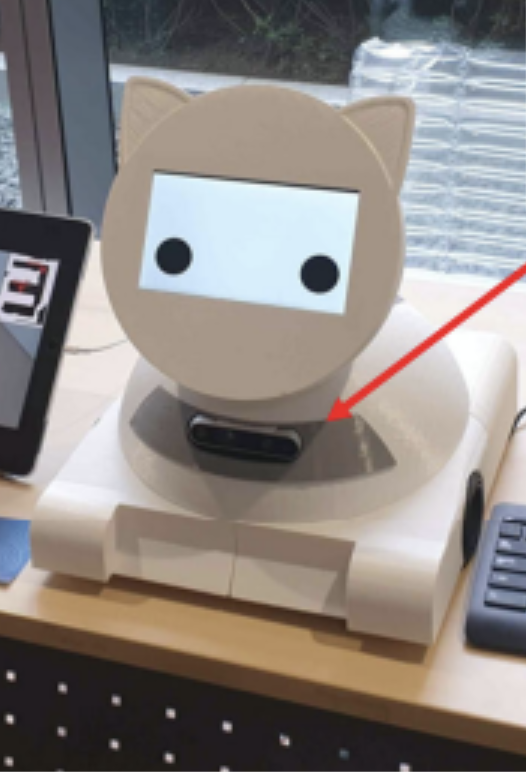
\includegraphics[scale=0.6]{dpoom.png}
    \caption*{Fonte: Adaptado de \citet{dpoom}.}
    \label{fig:dpoom}
\end{figure}

Os principais resultados encontrados em \citet{dpoom} são i) a taxa de operação reduzida,  de apenas 18Hz, para o algoritmo de navegação sem colisão com obstáculos; ii) a taxa baixa de 15\% de colisão; iii) a navegação bem sucedida em ambientes lotados.

\section{Robô Autônomo Móvel com LiDaR e RGB-D}
Em \citet{lidarRGBD},  é proposto um robô autônomo móvel (Figura~\ref{fig:lidarRGBD}) com maior percepção do ambiente, a fim de obter uma navegação mais eficiente ao evitar obstáculos dinâmicos e ser mais seguro a humanos e seus pertences. Para isso, foram implementados, em conjunto, um sensor LiDaR e uma câmera RGB-D para a percepção do ambiente. 

\begin{figure}[H]
    \centering
    \caption{Estrutura física do robô autônomo móvel com LiDaR e RGB-D}
    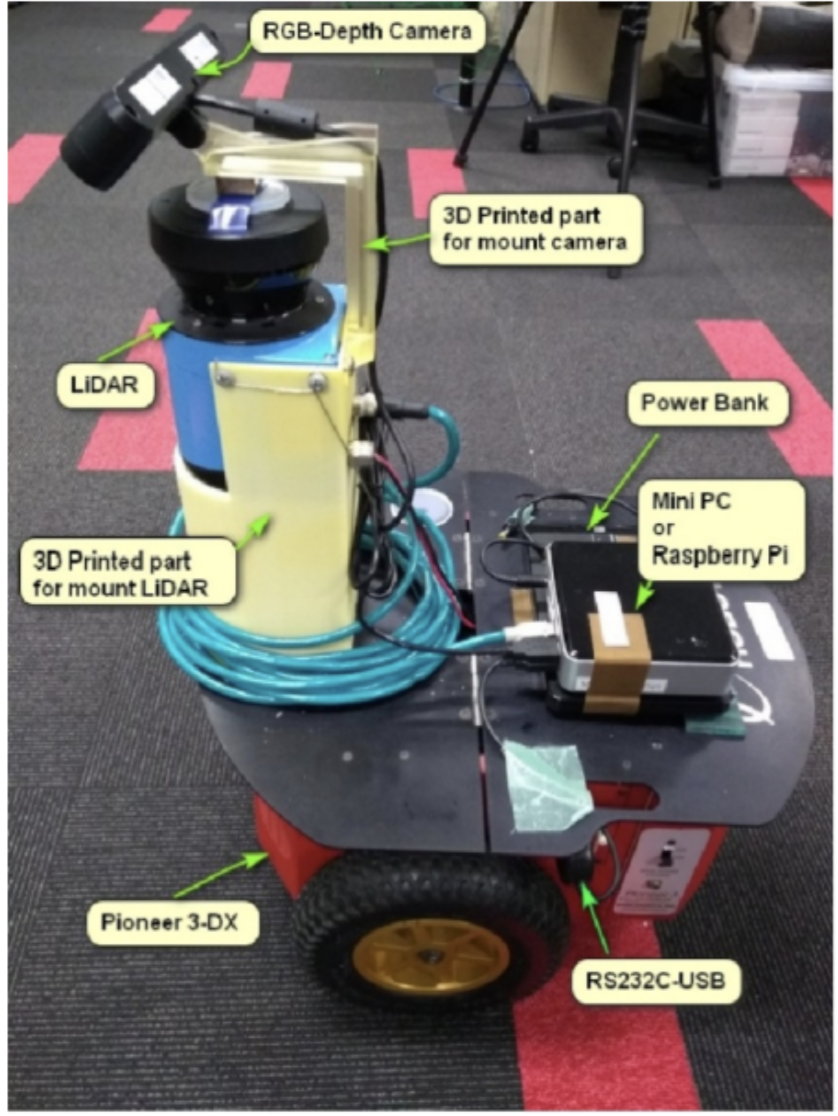
\includegraphics[scale=0.45]{lidarRGBD.png}
    \caption*{Fonte: \citet{lidarRGBD}.}
    \label{fig:lidarRGBD}
\end{figure}

Os instrumentos de percepção acima foram integrados para serem utilizados com o módulo de navegação do sistema ROS. Além disso, \citet{lidarRGBD} implementou uma biblioteca de mapeamento com SLAM do ROS para criar um mapa estático de duas dimensões do ambiente, utilizado em conjunto com o algoritmo AMCL para a localização do robô no ambiente. 

Para analisar o comportamento do robô desenvolvido, \citet{lidarRGBD} testou as suas integrações no simulador Gazebo com diferentes cenários que constituíam de obstáculos em posições e alturas variadas. Com isso, foi possível identificar que a câmera RGB-D permite capturar obstáculos mais altos, mas adiciona um custo de processamento para as informações de profundidade capturadas.

\section{Análise dos Trabalhos Correlatos}

A análise acima de alguns projetos correlatos ao presente trabalho proporcionou um conhecimento mais amplo sobre as possibilidades de implementação de soluções no contexto de robôs de serviço doméstico e navegação autônoma. Com isso, foi possível levantar uma tabela (Tabela~\ref{tab:trabalhosCorrelatos}) com as principais diferenças entre esses projetos conforme as tecnologias implementadas, estrutura física utilizada e considerações finais relevantes ao trabalho em questão. 

\begin{table}[H]
\caption{Principais características dos trabalhos correlatos comparados com AtmosBot}
\label{tab:trabalhosCorrelatos}
\resizebox{\textwidth}{!}{%
\begin{tabular}{p{5cm}|p{5cm}|p{5cm}|p{5cm}}
\multicolumn{1}{c|}{\textbf{Trabalho}} &
  \multicolumn{1}{c|}{\textbf{Principais Tecnologias}} &
  \multicolumn{1}{c|}{\textbf{Estrutura Física}} &
  \multicolumn{1}{c}{\textbf{Considerações Finais}} \\ \hline
Robô Herbert de \citet{herbert:1988} &
  Arquitetura de Subsunção. &
  3 rodas padrão, componentes altamente modularizados, sensor infravermelho e scanner de alcance a laser. &
  Uso de sensor infravermelho impacta negativamente o desempenho. \\ \hline
Robô Justina de \citet{justina:2019} &
  Arquitetura VIRBOT em conjunto com ROS e técnica SLAM para navegação. &
  2 rodas omnidirecionais, câmera Kinect Microsoft, câmera RGB e sensor laser. &
  A locomoção por rodas onidirecionais precisa ser melhorada. \\ \hline
Robô Turtlebot3 Burger de \citet{navegacaoSlam:2022} &
  SLAM aprimorado com Localização Adaptativa de Monte Carlo, em conjunto com ROS. &
  Sensor laser LIDAR. & A navegação é resiliente. \\ \hline
Robô DPoom de \citet{dpoom} &
  Sistema ROS e navegação combinada com SLAM e aprendizado profundo reforçado. &
  Câmera RGB-D. &
  Menos custoso em processamento e recursos. \\ \hline
Robô com LiDaR e RGB-D de \citet{lidarRGBD} &
  SLAM e algoritmo AMCL, integrados com ROS. &
  Sensor LiDaR, câmera RGB-D. & 
  Mais obstáculos capturados, mas maior custo de processamento. \\ \hline
  AtmosBot &
  SLAM com mapeamento simultâneo a exploração e biblioteca de navegação, integrado com ROS e arquitetura de subsunção. &
  Sensor LiDaR e 4 rodas padrão. & 
  Menor custo de processamento e mapeamento menos divergente.
\end{tabular}
%
}
\caption*{Fonte: Autora (2023).}
\end{table}

Diante das informações supracitadas, é possível identificar certas similaridades entre os trabalhos expostos e suas principais diferenças. Assim como no AtmosBot, a abordagem de localização e mapeamento mais utilizado é o SLAM, conforme implantado nos robôs de \citet{justina:2019}, \citet{navegacaoSlam:2022}, \citet{dpoom}, \citet{lidarRGBD}. Para a percepção do ambiente,  os instrumentos mais recorrentes são a câmera RGB e o sensor LiDaR, sendo o último mais utilizado, assim como no AtmosBot. Por fim, a simulação foi utilizada na maioria das pesquisas para a validação parcial ou completa do sistema desenvolvido e os elementos do robô foram integrados pela arquitetura ROS, ambos aspectos presentes no AtmosBot.

As diferenças mais destacáveis entre os trabalhos são os algoritmos mais específicos de localização e de evitar obstáculos, existindo entre eles o AMCL e o aprendizado profundo reforçado. No AtmosBot, nenhum desses algoritmos são utilizados visto que foram implementadas as bibliotecas de navegação do ROS que dispõe o processo de localização sem a necessidade de maiores complementos.

Portanto, a maior contribuição dos trabalhos correlatos analisados é gama de possibilidades existentes para o desenvolvimento de um robô autônomo móvel. Além disso, esses trabalhos expõem as vantagens do uso do ROS, para integrar todos os componentes de navegação, e do programa Gazebo, para realizar as validações necessárias. Essas contribuições são consideradas ao elaborar a proposta da solução, conforme explicado no próximo capítulo que trata sobre o desenvolvimento do modelo proposto.

\chapter{Desenvolvimento}
\label{cap-desenvolvimento}
Neste capítulo são apresentados a proposta do presente trabalho, as especificações e modelagem levantadas para a solução, além dos detalhes de desenvolvimento do modelo para o robô AtmosBot.

\section{Proposta de Solução do AtmosBot} 

A partir do que foi explicado anteriormente, se conclui que um robô de serviço doméstico é um sistema complexo que,  para ser desenvolvido, demanda uma abundância de recursos, tempo e profissionais. Assim, surge a necessidade de elaborá-lo de forma modular, se beneficiando de testes simulados para minimizar os recursos financeiros e o tempo despendido. Logo, este trabalho propõe um modelo simulado para a funcionalidade primordial do robô de serviço doméstico: a navegação autônoma. Com isso, foi elaborado um modelo simulado de robô autônomo móvel capaz de navegar, sem interferência humana, por um ambiente interno dinâmico, similar a um domicílio. 

Foram identificadas as tecnologias relevantes e vantajosas para desenvolver o robô autônomo móvel. Essas tecnologias tratam sobre as funcionalidades: i) simulação do modelo; ii) a localização, percepção e locomoção do robô; iii) abordagem do controle lógico. Assim, a seguir são apresentadas as tecnologias escolhidas para o desenvolvimento do modelo proposto.

%%SIMULADOR-------
A simulação do modelo proposto foi realizada a partir da plataforma Gazebo. Dentre os simuladores mais utilizados atualmente, sendo eles o WeBot, Gazebo e CoppeliaSim, o Gazebo apresenta a melhor adequação para o presente trabalho, conforme os resultados obtidos pelo experimento comparativo dos simuladores realizado por \citet{pickSimulatorFarley:2022}. As principais vantagens do Gazebo são a utilização ampla perante os desenvolvedores e designers de robótica, a gratuidade do programa e a comunidade ativa que possibilita uma maior facilidade na resolução de possíveis problemas para sua instalação e o seu uso \cite{gazeboDesigns:2004, pickSimulatorFarley:2022}. 

%%NAVEGAÇÃO------- 
No âmbito da navegação autônoma, diferentes abordagens podem ser utilizadas em conjunto para implementar cada sub-tarefa que constitui a navegação de um robô autônomo móvel. Ao todo, foram necessárias lógicas que possibilitem que o robô vague, explore e se localize pelo ambiente de forma inteligente, com menor quantidade de colisões e sem a interferência de humanos.

A pesquisa bibliográfica para identificar as abordagens mais relevantes para a localização do robô resultou em 4116 publicações totais do tema, obtendo  42 artigos finais coerentes com os critérios de inclusão. Os resultados intermediários, conforme os momentos pré-estabelecidos, podem ser encontrado na Figura~\ref{fig:diagramaResultadosLocalizacao}. 

\begin{figure}[h]
    \centering
    \caption{Resultado completo da pesquisa bibliográfica de abordagens para localização de robôs autônomos móveis}
    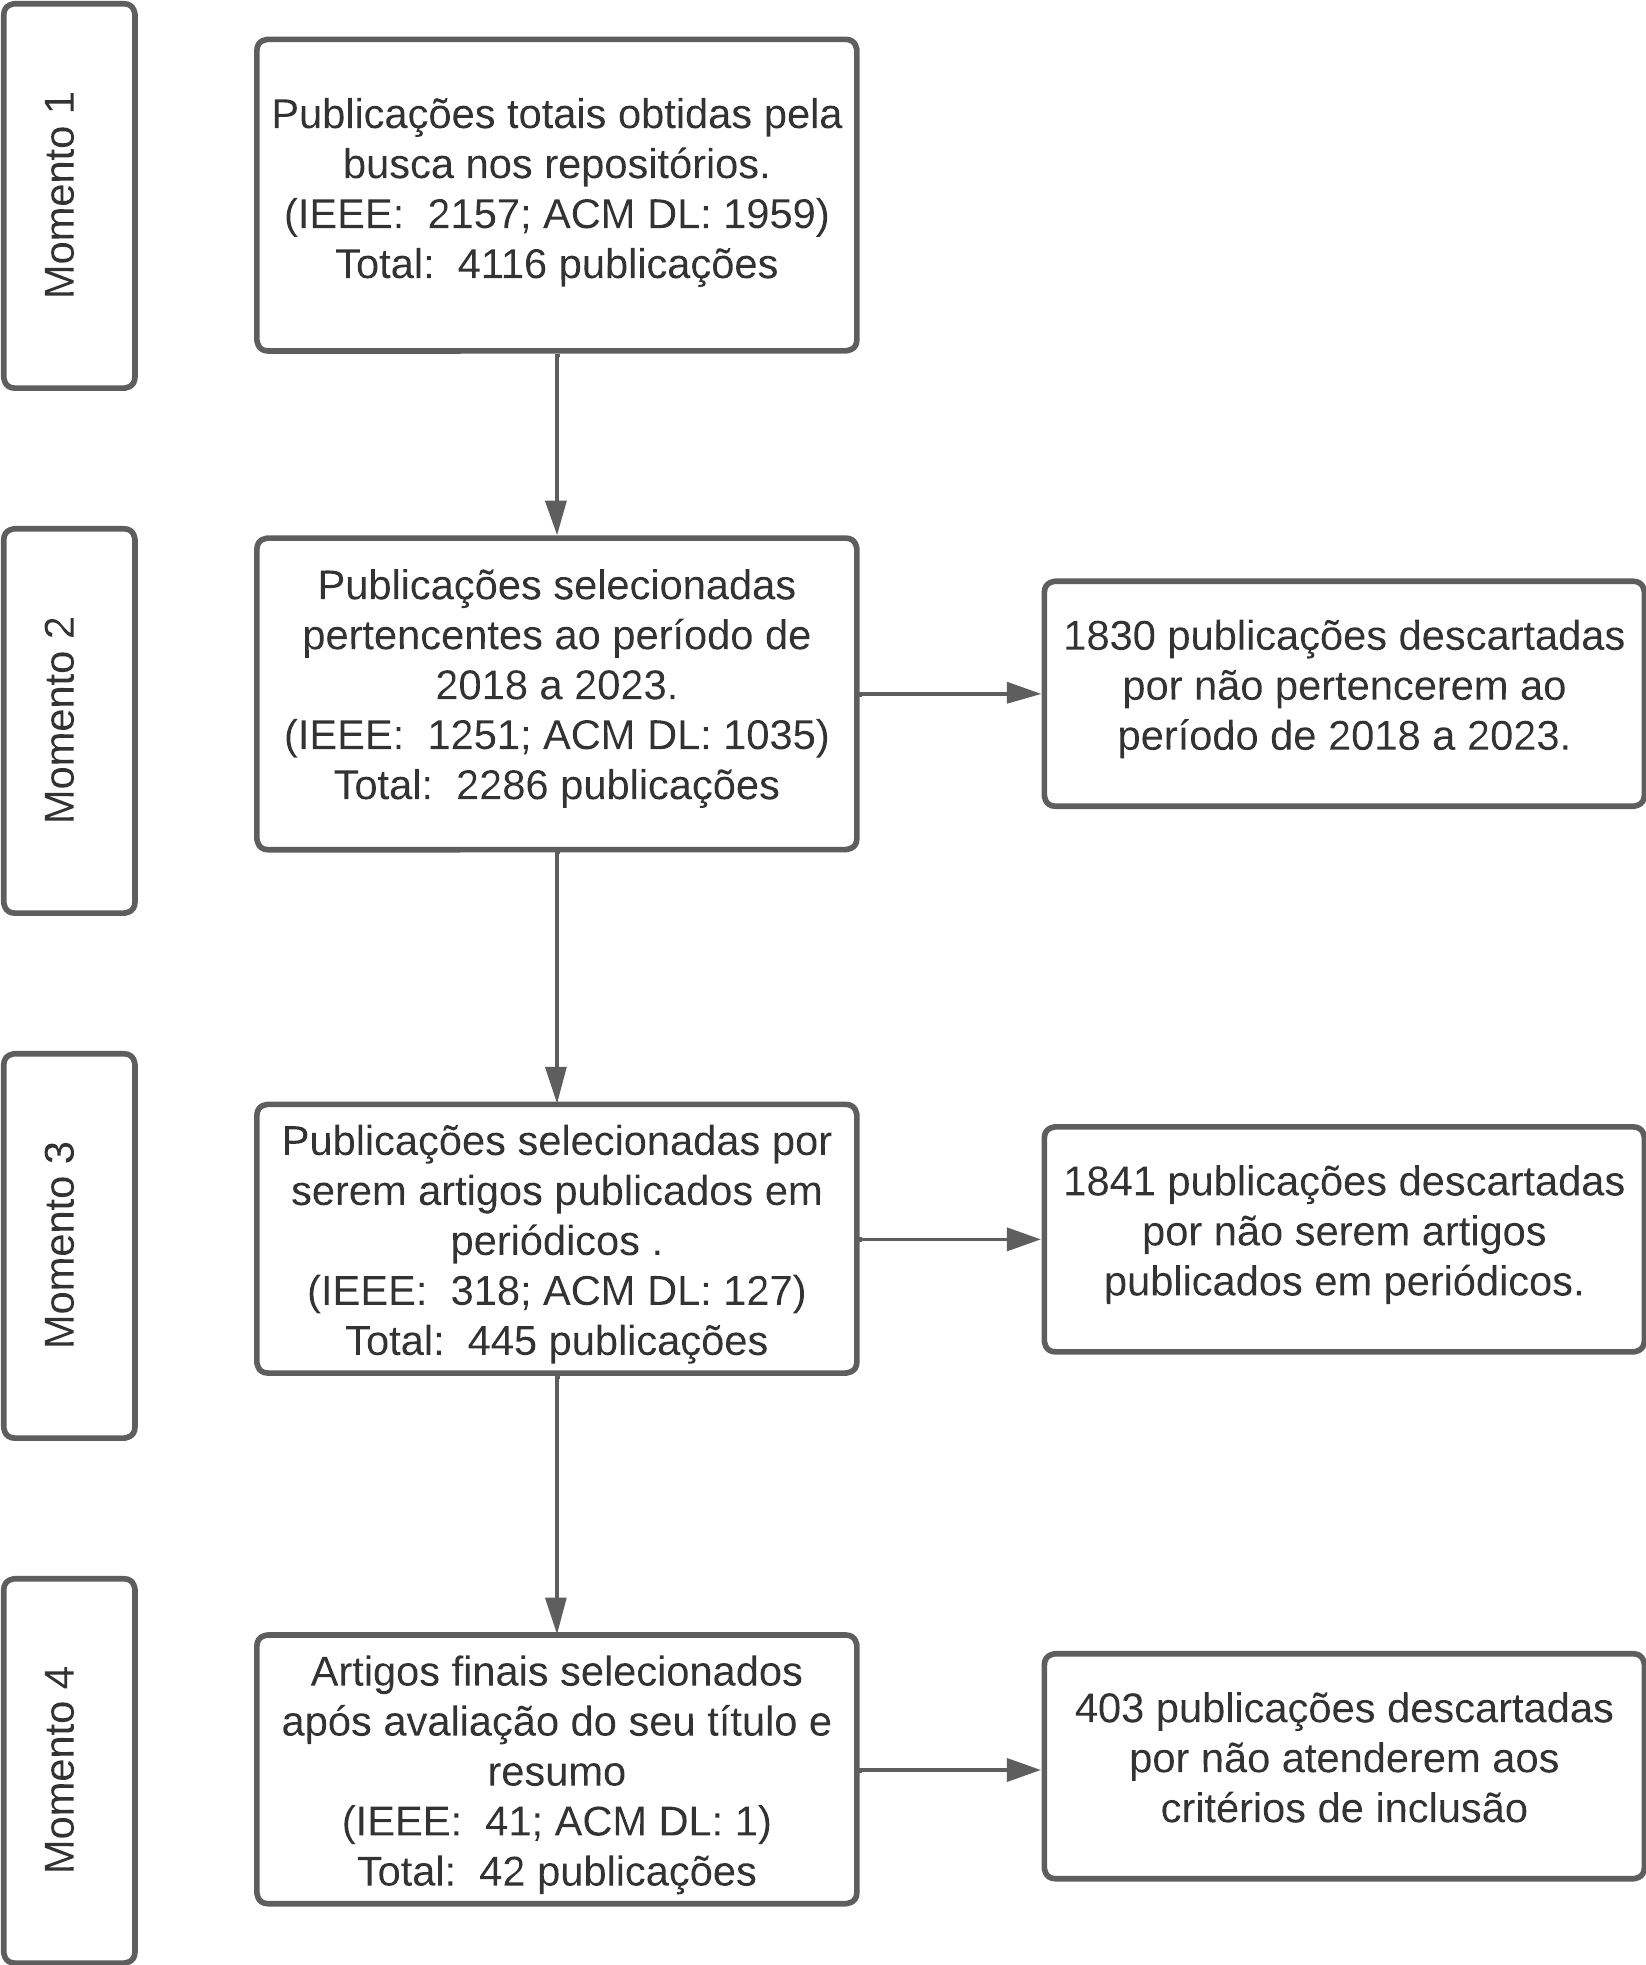
\includegraphics[scale=0.8]{diagramaResultadosLocalizacao.png}
    \caption*{Fonte: Autora (2023).}
    \label{fig:diagramaResultadosLocalizacao}
\end{figure}

Dentre as abordagens encontradas para localização de robôs autônomos móveis, 25 deles utilizavam a abordagem SLAM, pura ou com incrementos para melhorar o seu desempenho. No gráfico abaixo (Figura~\ref{fig:graficoPesquisaLocalizacao}) é possível observar todas as abordagens implementadas para a localização do robô em um ambiente interno, obtidas pela pesquisa realizada. Portanto, foi utilizado o algoritmo de localização e mapeamento simultâneo (SLAM) para auxiliar o robô a navegar de forma inteligente.

\begin{figure}[h]
    \centering
    \caption{Resultado da pesquisa bibliográfica de abordagens para localização de robôs autônomos móveis}
    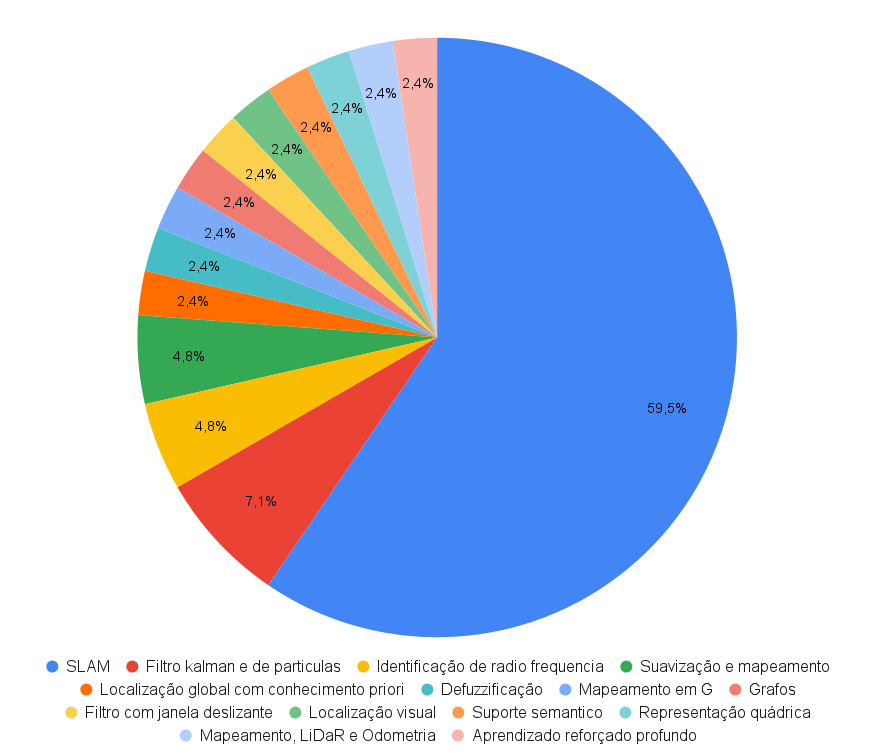
\includegraphics[scale=0.37]{resultadosAlgLocalizacao.png}
    \caption*{Fonte: Autora (2023).}
    \label{fig:graficoPesquisaLocalizacao}
\end{figure}

%%PERCEPÇÃO-----
De forma similar, a pesquisa bibliográfica que visava responder qual o instrumento mais utilizado para a percepção do ambiente pelo robô autônomo móvel, resultou em 1501 publicações totais, obtendo 33 artigos finais coerentes com os critérios de inclusão e exclusão definidos. Os resultados intermediários, conforme os momentos pré-estabelecidos, podem ser encontrado na Figura~\ref{fig:diagramaResultadosPercepcao}. 

\begin{figure}[h]
    \centering
    \caption{Resultado completo da pesquisa bibliográfica de instrumentos de percepção do ambiente}
    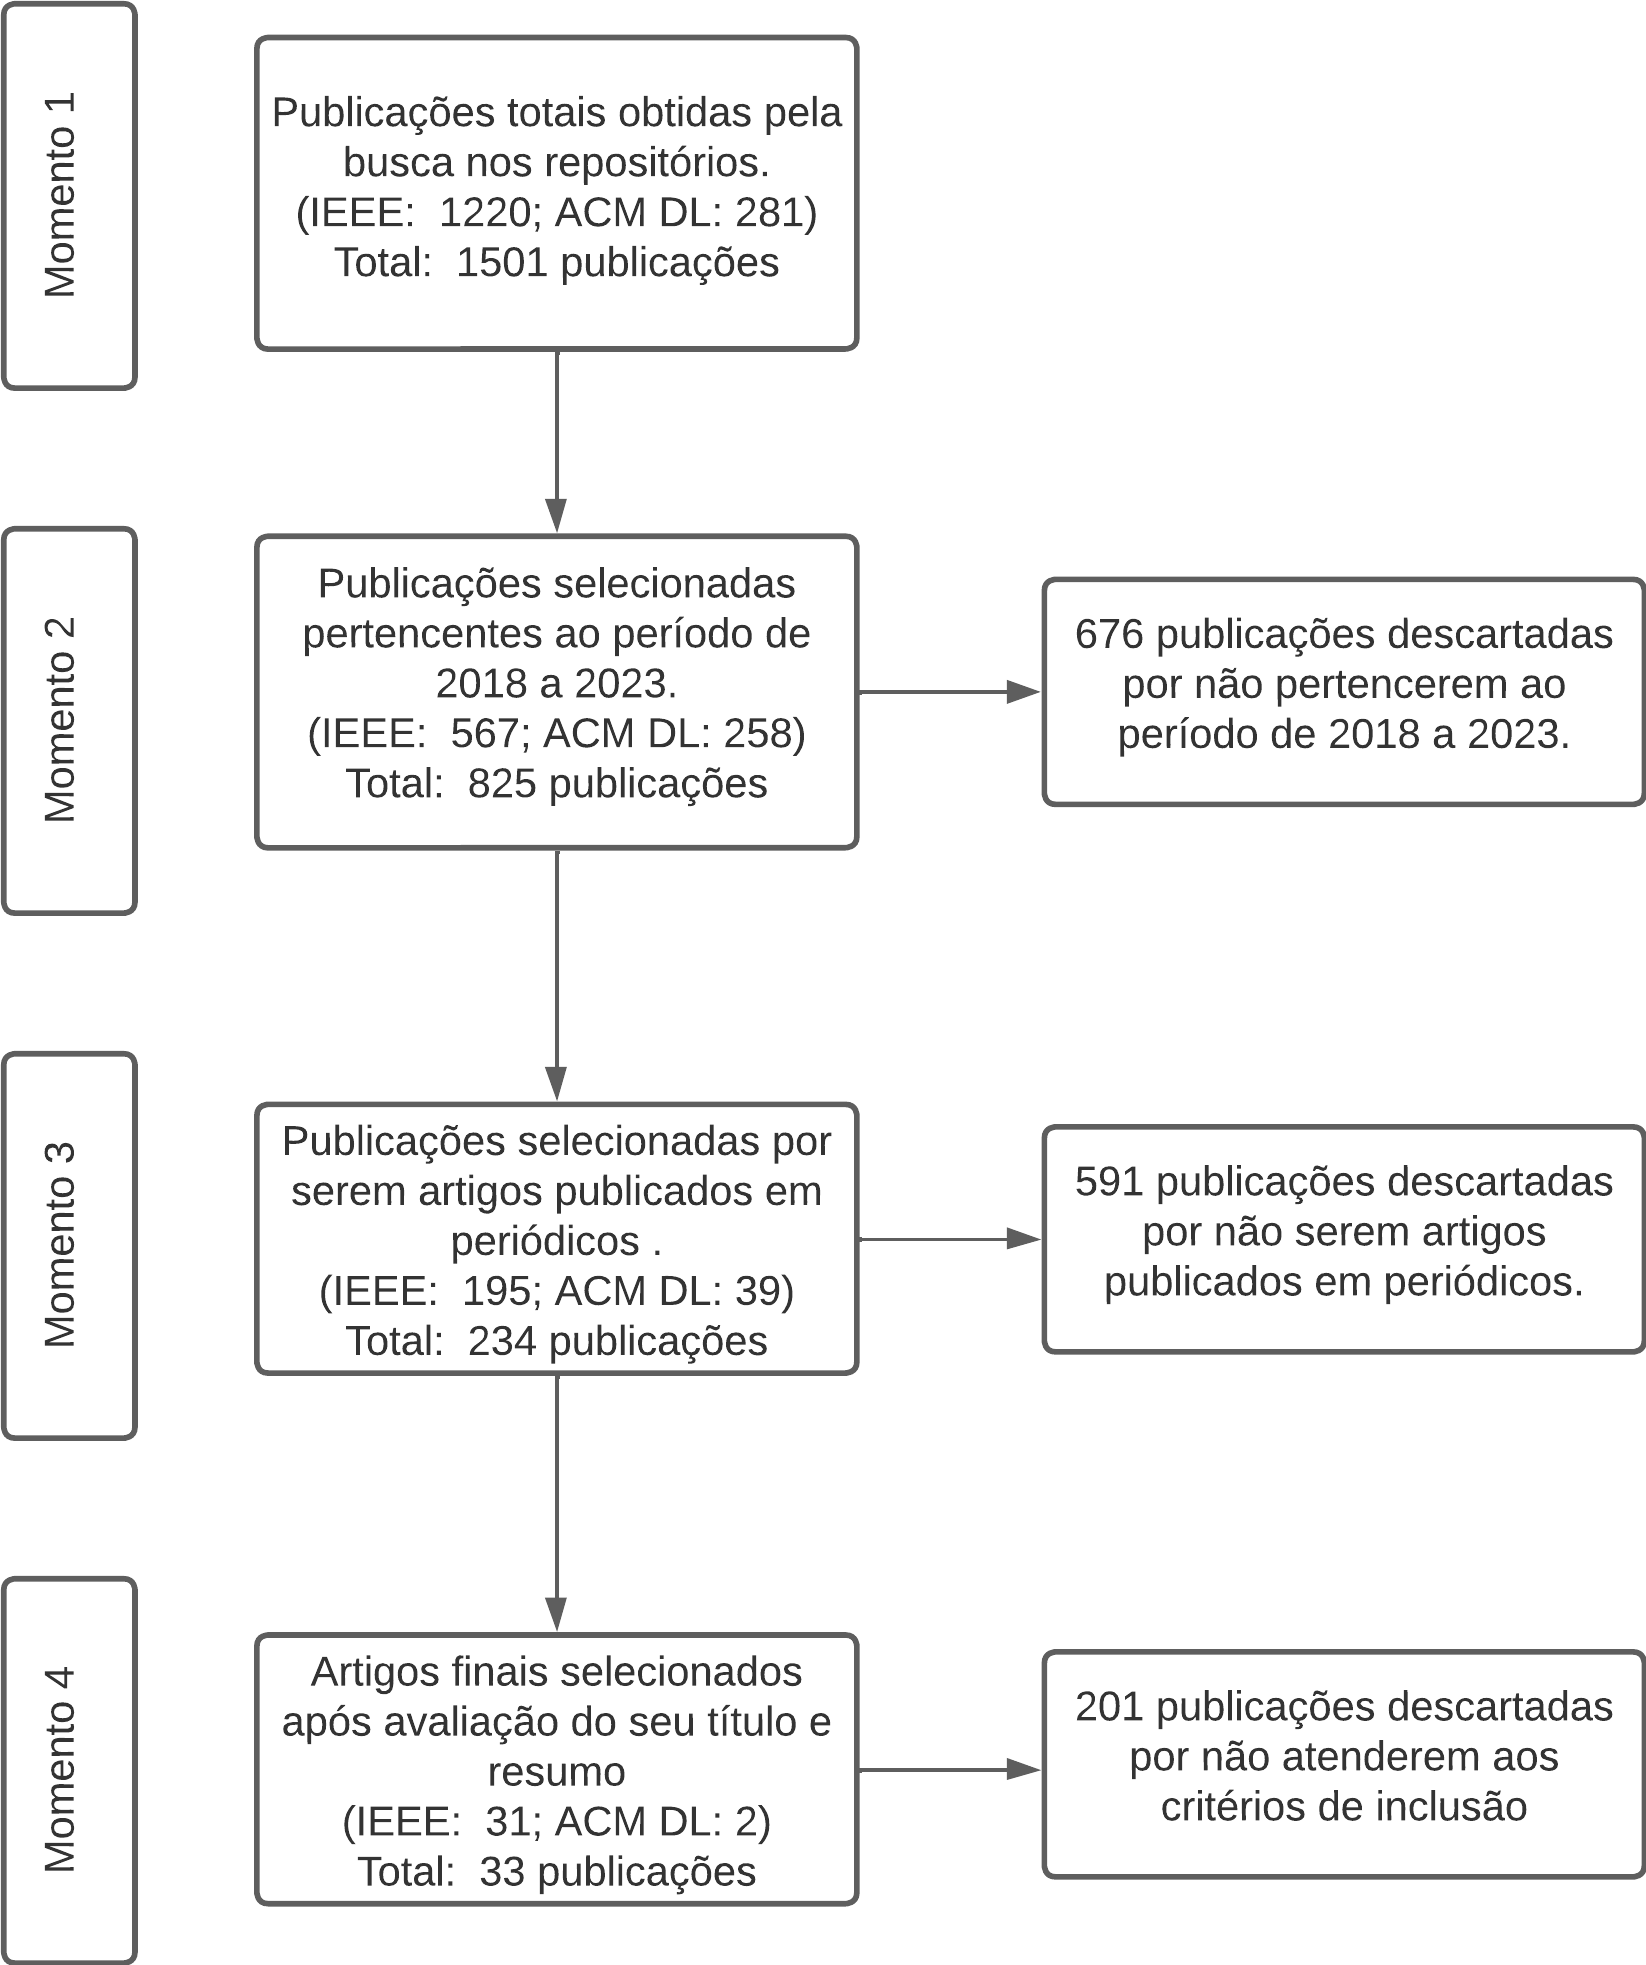
\includegraphics[scale=0.8]{diagramaResultadosPercepcao.png}
    \caption*{Fonte: Autora (2023).}
    \label{fig:diagramaResultadosPercepcao}
\end{figure}

Dentre as 33 publicações encontradas por essa pesquisa bibliográfica, 14 delas utilizam o sensor LiDaR e 5 utilizam a câmera, para o robô compreender o ambiente ao redor (Figura~\ref{fig:graficoPesquisaPercepcao}). Logo, foi optado a integração do sensor LiDaR para que o robô colete informações precisas do meio em que se encontra.

\begin{figure}[h]
    \centering
    \caption{Resultado da pesquisa bibliográfica de instrumentos de percepção do ambiente}
    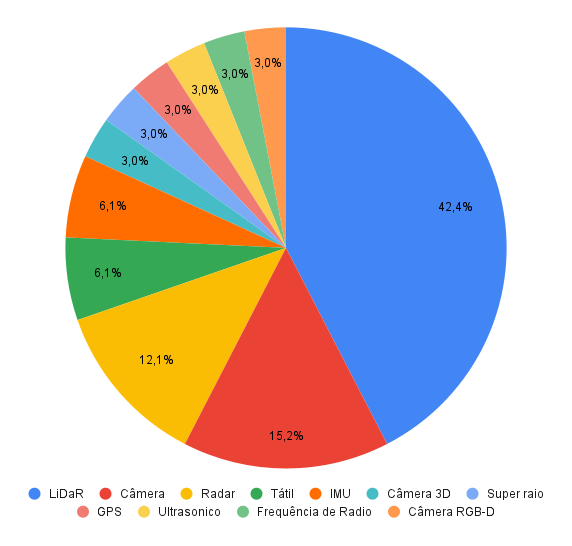
\includegraphics[scale=0.55]{resultadosPercepcao.png}
    \caption*{Fonte: Autora (2023).}
    \label{fig:graficoPesquisaPercepcao}
\end{figure}

%%LOCOMOÇÃO------- 
Como explicado anteriormente, a locomoção dos robôs autônomos móveis pode ser realizada com rodas ou pernas, similarmente a animais. Para o presente trabalho, foi optado utilizar rodas, ao apresentar uma melhor eficiência energética e não requerer técnicas para garantir equilíbrio do corpo do robô durante a movimentação, apresentando ser uma alternativa mais minimalista e intuitiva em sua concepção e implementação.  Com isso, o AtmosBot possui de 4 rodas de design padrão, dispostas a formar um quadrado na base do robô.

Como exposto no \chapterautorefname~\ref{cap-revisao-bibliografica}, o controle lógico do robô pode ser implementado com duas abordagens antagônicas: a inteligência artificial clássica sequencial e a arquitetura de subsunção com paralelismo. A fim de obter um robô com contato direto com as informações do ambiente em todos os seus módulos independentes, maior robustez, com capacidade de futuras incrementações, além de maior resiliência e menor tempo de resposta a mudanças no ambiente, foi optado o uso da arquitetura de subsunção, com um grau de liberdade para possíveis adaptações necessárias caso demonstre ser mais adequado para a proposta.

Por fim, o ambiente também deve ser definido para que o modelo do robô seja correto. Esse robô deve atuar em um ambiente interno e dinâmico, semelhante a um domicílio acessível. Ou seja, o robô consegue atuar apenas em ambientes com uma iluminação controlada, com obstáculos  (parede, portas fechadas, móveis e outros objetos), com  mudanças na disposição dos artefatos presentes, além de não possuir degraus com altura acima de 1 centímetro.

\section{Especificação de Requisitos}

Os requisitos de um sistema são características que esse sistema necessita para o seu funcionamento. Os requisitos básicos devem ser identificados previamente ao desenvolvimento, no intuito de compreender ao máximo os limites do sistema e as funcionalidades que devem ser alcançadas \cite{pressman}.

Dito isso, foi  levantada uma série de requisitos do sistema completo, incluindo a simulação do ambiente e do robô proposto. Esse conjunto de requisitos levantados detalham as possíveis ações do robô e suas características mais intrínsecas, além de conformidades do ambiente. 

Em específico, foram levantados requisitos funcionais e não funcionais para o robô autônomo móvel proposto. Essas especificações abordam a movimentação do robô ao longo da sua trajetória no ambiente, como sua capacidade de evitar os obstáculos e conter uma velocidade segura para os humanos e a propriedade presente no meio inserido.

Ademais, foram levantados requisitos não funcionais para o ambiente, explicitando as necessidades do local de atuação do robô proposto. Dentre elas, foram destacadas a verossimilhança com domicílios comuns e sua dinamicidade como um meio convivido por seres.

A fim de expor todos os requisitos, foi elaborado um documento de Especificação de Requisitos do Sistema  com base nas práticas recomendadas pela norma IEEE Std 830-1998, Práticas Recomendadas para Especificações de Requisitos de Software da IEEE,  que pode ser encontrado na íntegra no \appendixautorefname~\ref{appendix-requisitos}.

\section{Modelagem do Sistema}

O AtmosBot como navegador autônomo cumpre seu objetivo de navegação eficiente a partir de duas grandes etapas: espera no ponto de partida e exploração do ambiente

A exploração do ambiente pode ser subdividida em quatro tarefas importantes executadas paralelamente: 1) a locomoção pelo espaço, 2) a coleta de informações do meio para se localizar, 3) o mapeamento do ambiente, 4) o desvio dos obstáculos fixos e dinâmicos. Todas essas funcionalidades podem ser caracterizadas por estados conforme demonstrados na Figura~\ref{fig:estados}. 

\begin{figure}[h]
    \centering
    \caption{Estados principais do AtmosBot}
    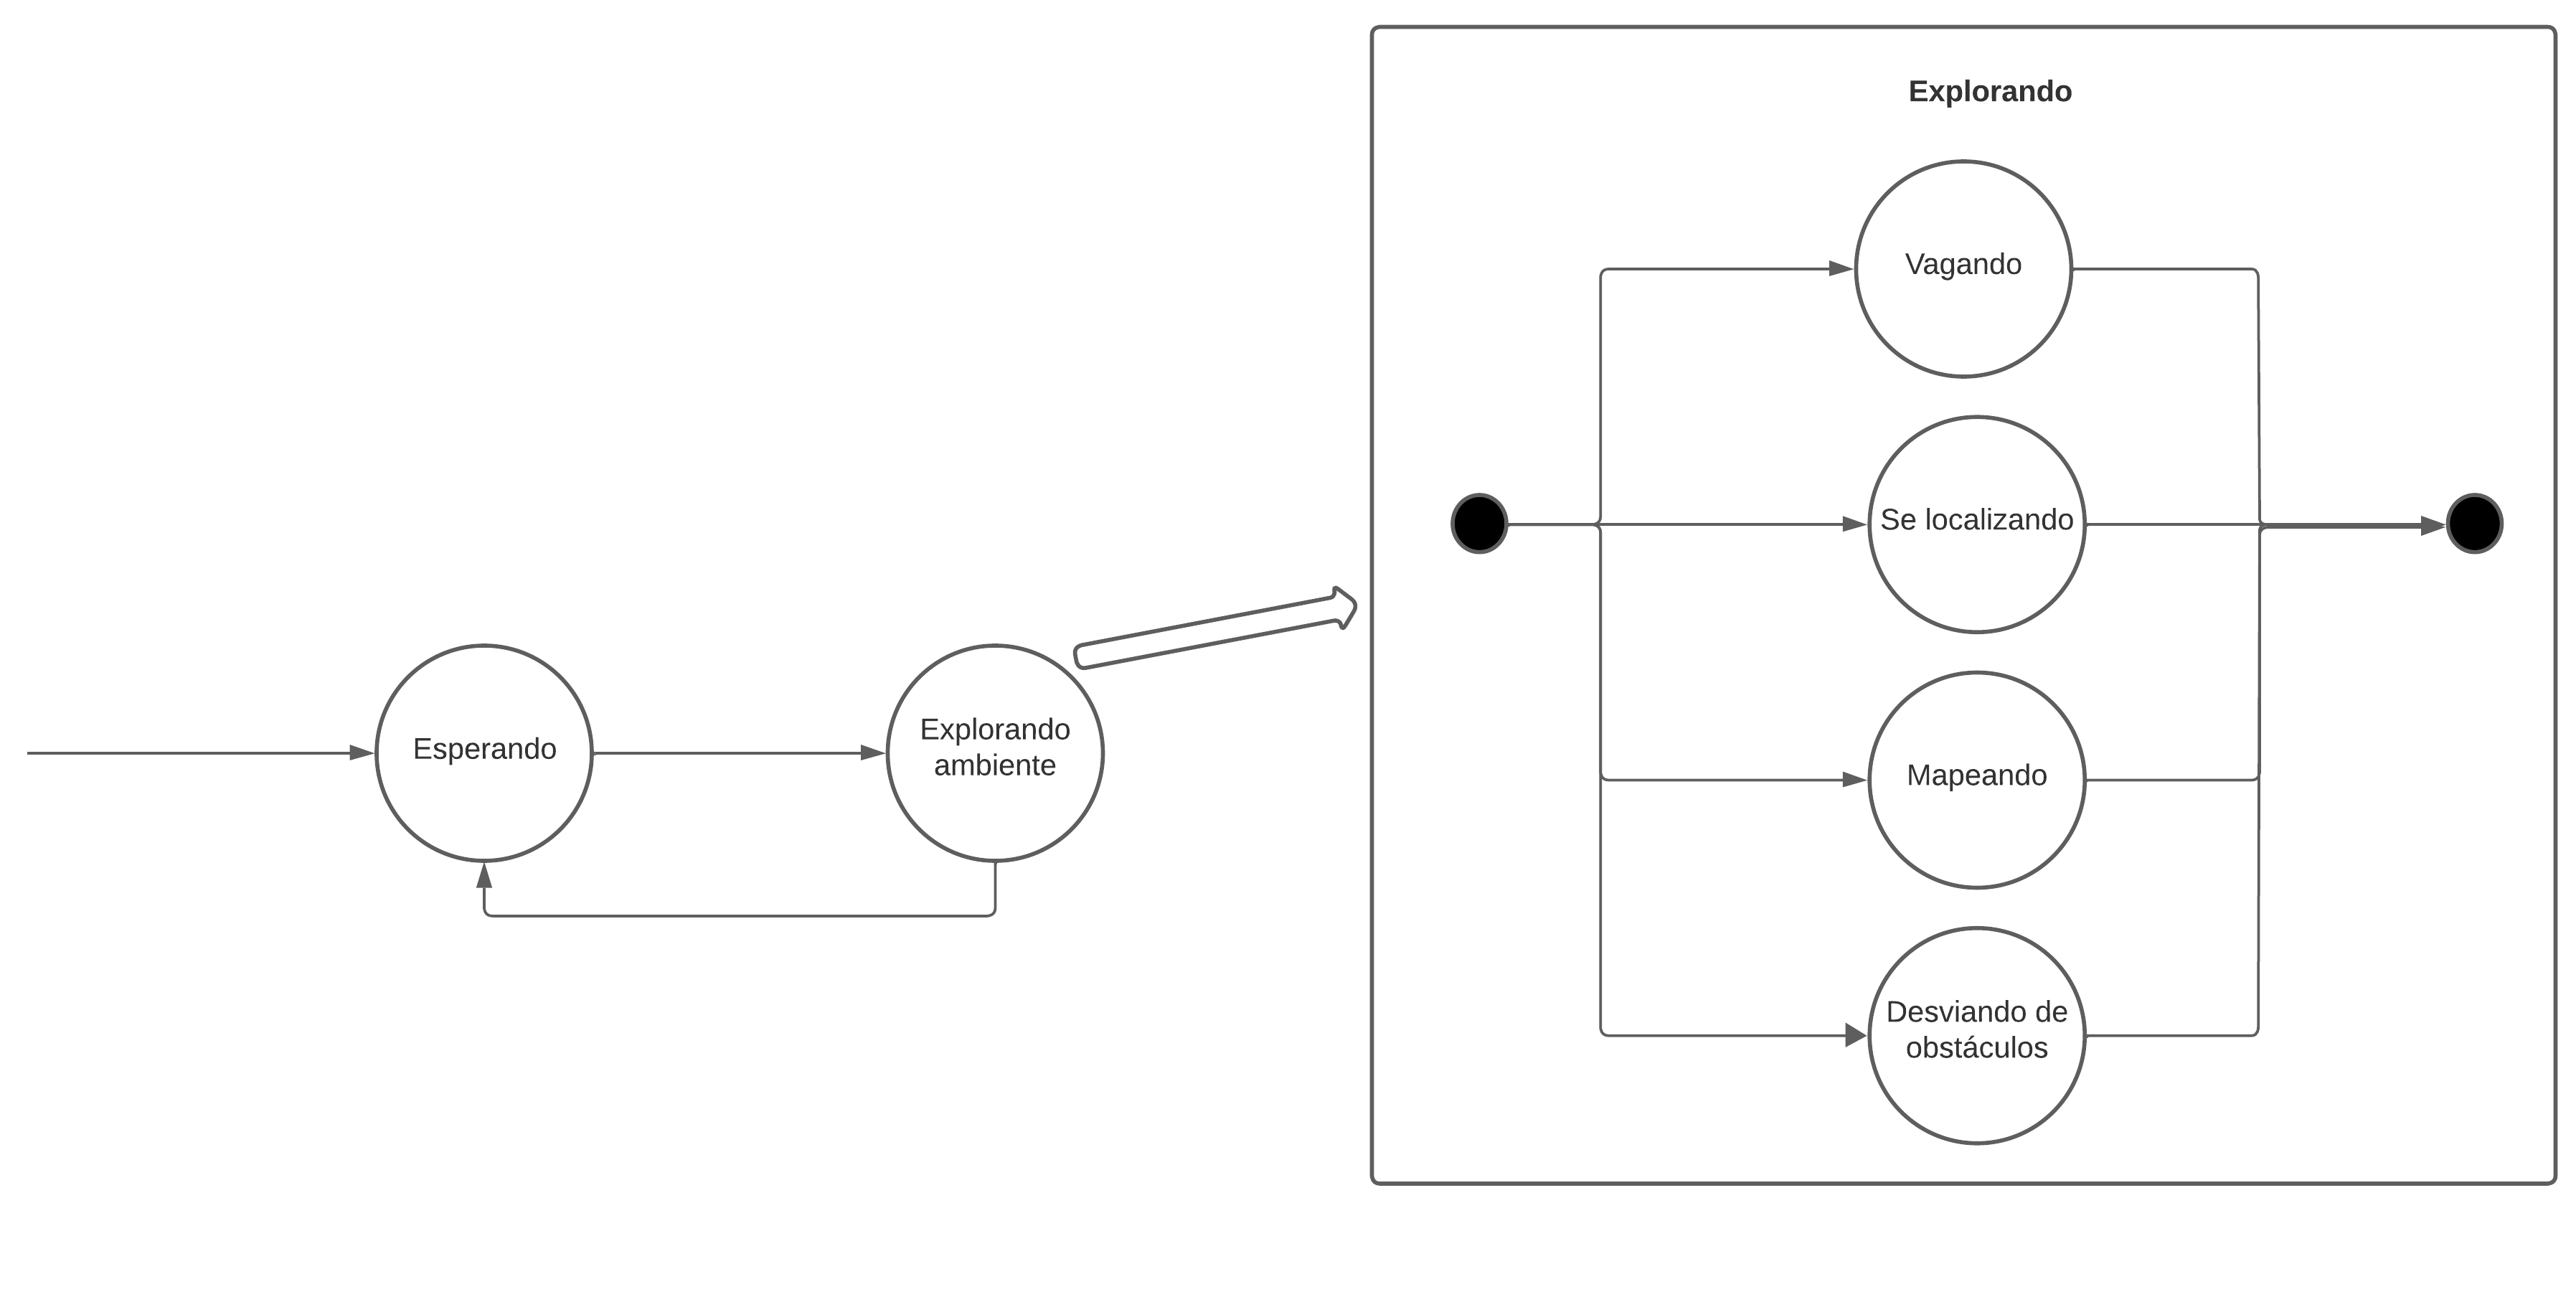
\includegraphics[scale=0.45]{estados.png}
    \caption*{Fonte: Autora (2023).}
    \label{fig:estados}
\end{figure}


Inicialmente, o sistema deve estar em modo de espera para começar sua tarefa. Passado o tempo padrão de espera para que todos os seus processamentos estejam preparados, o robô inicia sua tarefa de explorar o ambiente, vagando pelo meio sem colidir com os obstáculos e coletando informações sobre a sua posição. 

Este modelo permite a adição de outras funcionalidades em paralelo com o módulo de navegação, conforme a aplicação da abordagem de subsunção, que torna as unidades independentes. Apesar de serem unidades independentes, o módulo de navegação autônoma e outros possíveis módulos devem ser interligados com transmissão de informações cruciais entre si, além de se comunicarem com o próprio ambiente onde o robô se encontra. Essa interação entre os subsistemas, o sistema geral e o ambiente, pode ser analisada visualmente através da Figura~\ref{fig:blocos}.  

Em paralelo com a execução de outras possíveis funcionalidades que poderão ser incrementadas, o módulo de navegação recebe as informações que os instrumentos de percepção coletam do ambiente e as suas sub-camadas utilizam esse conhecimento para definir a atividade dos atuadores (os motores e consequentemente as rodas). Uma vez que o robô atua no ambiente, as informações dele mudam, pois o robô se encontra em outra posição, tornando um ciclo fechado entre atuação e percepção do meio.

\begin{figure}[h]
    \centering
    \caption{Diagrama de blocos do modelo}
    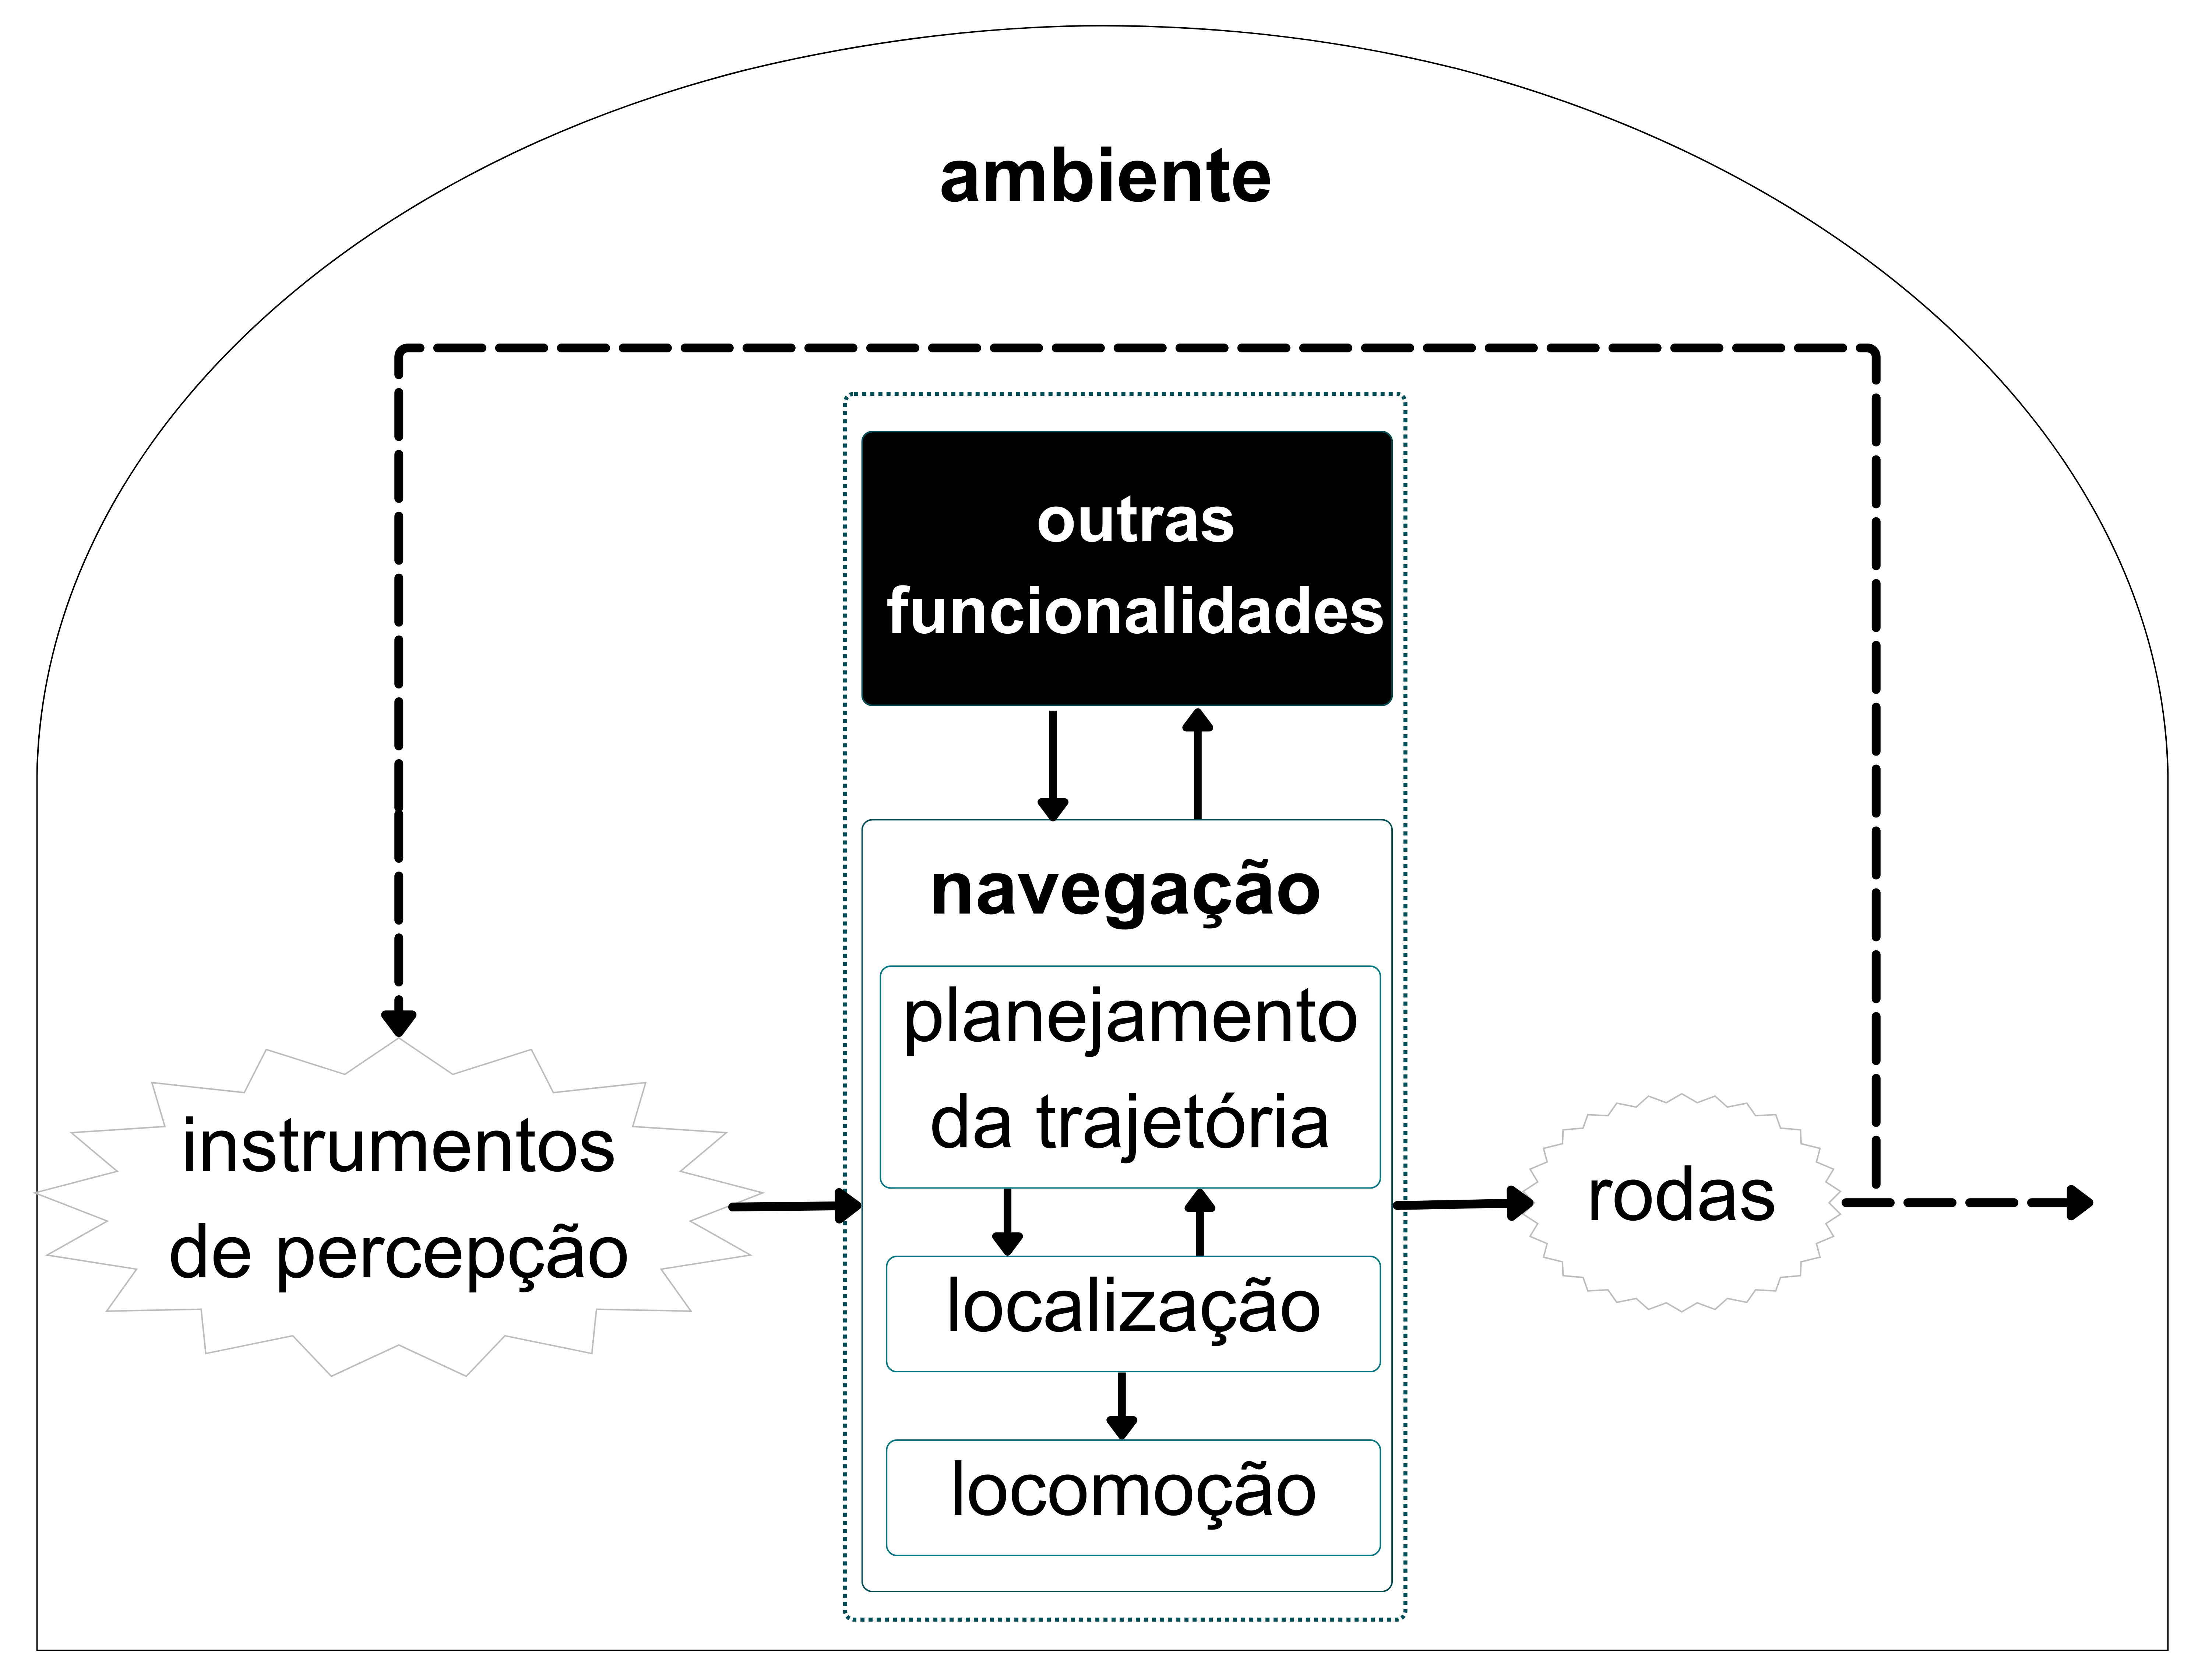
\includegraphics[scale=0.08]{blocos.png}
   
    \caption*{Fonte: Autora (2023).}
    \label{fig:blocos}
\end{figure}


\section{Implementação da Proposta}
A implementação da proposta pode ser separada em três elementos: i) a simulação; ii) o controle do robô; iii) integração de todos os componentes. O desenvolvimento de cada elemento é explicado detalhadamente a seguir.

\subsection{Simulação}
A simulação é responsável por permitir a recriação da realidade de forma mais verossímil possível. Para isso, cada aspecto dos elementos reais deve ser descrito com alta riqueza de detalhes, para serem representados na simulação com maior semelhança. Para o simulador Gazebo, essa descrição é realizada mediante arquivos SDF (do inglês Formato de Descrição de Simulação) que compõe todas as características necessárias para a definição de elementos do ambiente e do robô. Entre essas características, são descritas o comportamento dos componentes perante as leis da física, além de tamanho, cor, articulações e movimento.

Visto que uma das maiores vantagens do simulador Gazebo é a sua comunidade ativa de desenvolvedores usários que continuamente disponibiliza novos modelos de robôs e ambientes, foi possível criar o robô AtmosBot baseado no modelo disponibilizado por \citet{modeloRobo}. A fim de obter uma melhor resolução na simulação, em conjunto com os arquivos SDF, cada parte do robô (rodas, base e estrutura vertical) foi renderizada por dados de malha tridimensional (MESH) elaborados e modificados no programa de design 3D Blender.

Assim como o uso de um modelo de robô disponibilizado pela comunidade do Gazebo, foi possível montar o domicílio simulado com modelos publicados pela plataforma "AWS Robot Maker" da Amazon, destinada a executar e automatizar simulações sem necessitar lidar com a infraestrutura \cite{aws, modeloAmbiente}.

A simulação se torna completa ao combinar o ambiente montado com o robô elaborado. Para compreender a visão do robô ao longo da simulação, foi utilizado o programa RVIZ que permite visualizar os processos ocorrendo com o robô, como a sua odometria, velocidade e capturas de sensores.

\subsection{Navegação Autônoma}

A navegação autônoma do AtmosBot foi subdividida em duas principais partes: i) vagar pelo ambiente sem colisões e ii) mapeamento e localização durante exploração do ambiente.

A fim de fazer o robô se locomover pelo ambiente simulado de forma livre sem colidir com os móveis e paredes ao longo do caminho, foi desenvolvido um algoritmo, na linguagem C++, capaz de compreender obstáculos à sua frente. Para isso, são capturadas as leituras do sensor LiDaR, posicionado na dianteira do robô, com intuito de validar se existe um obstáculo à sua frente e os possíveis cenários para rotação do robô (Figura~\ref{fig:fluxogramaEvitarObstaculos}).  Uma vez que foi identificado uma nova rota, são definidas as velocidades linear (para seguir em frente ou dar ré) e angular (para rotacionar), conforme necessário.

\begin{figure}[h]
    \centering
    \caption{Fluxograma do algoritmo de vagar sem colidir}
    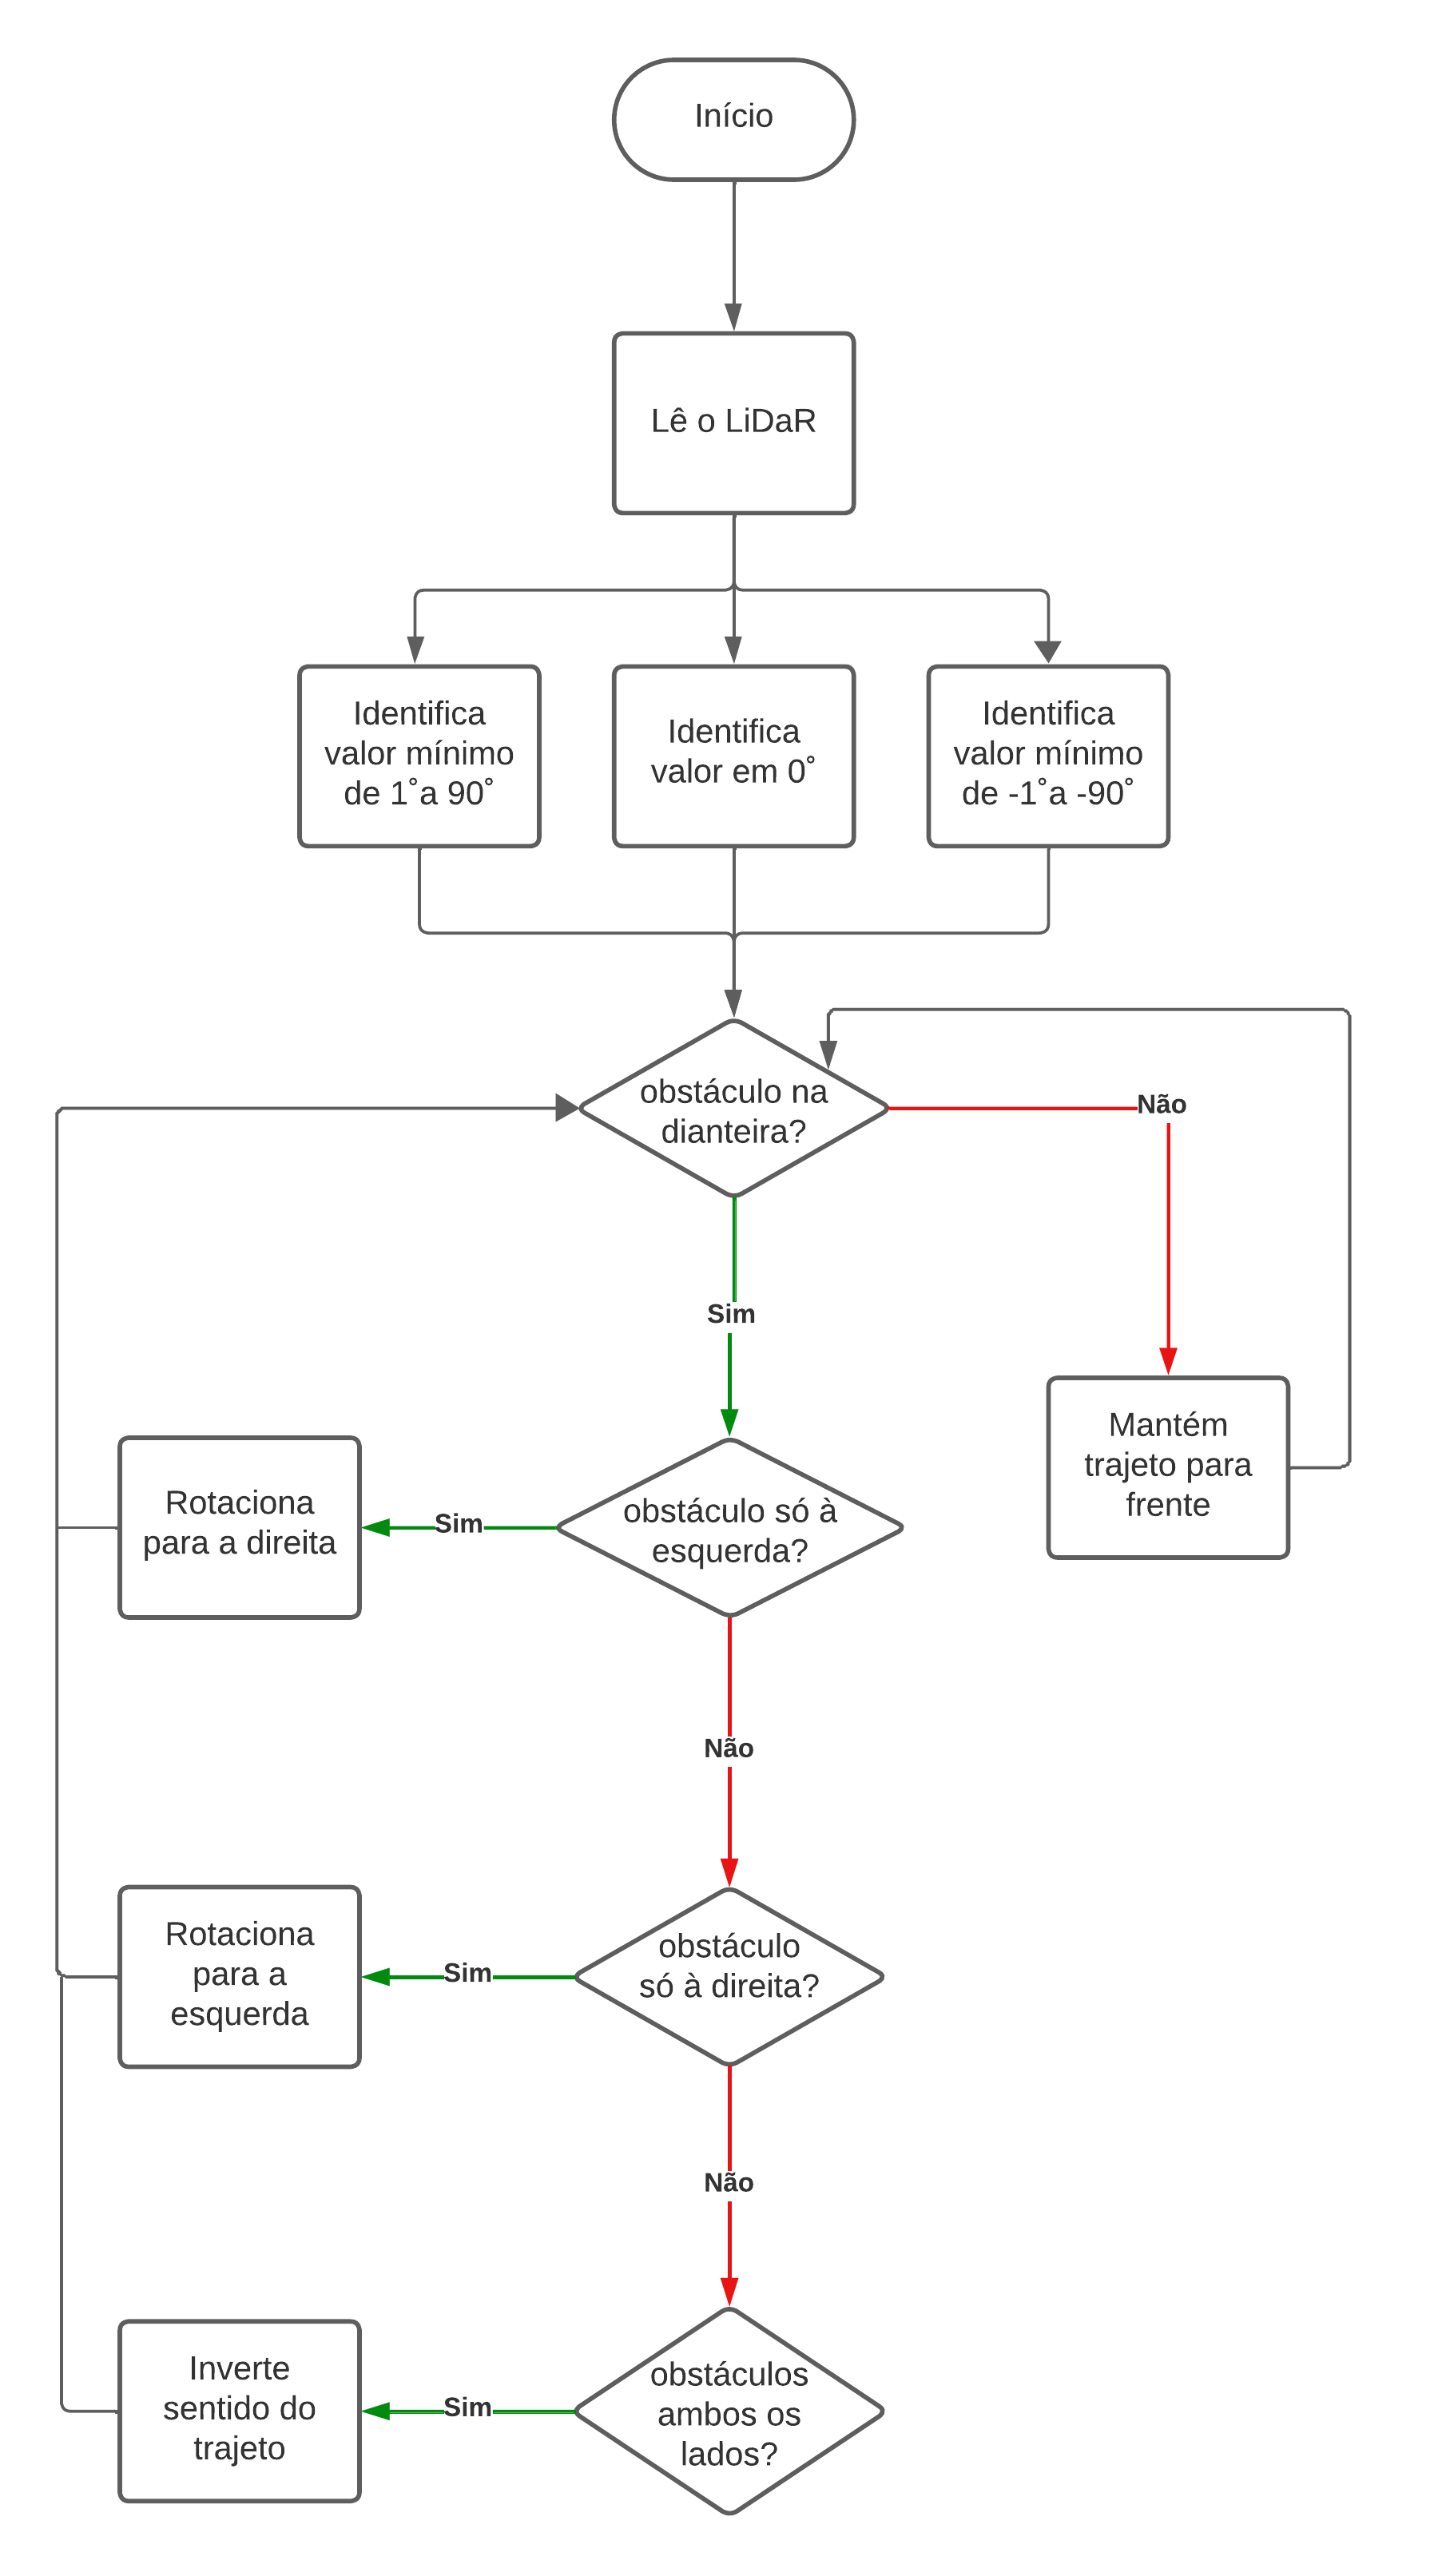
\includegraphics[scale=0.5]{fluxogramaEvitarObstaculos.png}
    
    \caption*{Fonte: Autora (2023).}
    \label{fig:fluxogramaEvitarObstaculos}
\end{figure}

Para o mapeamento do ambiente e a localização do robô, foi possível usufruir de uma das maiores vantagens do Sistema Operacional de Robô (ROS): as variadas bibliotecas disponíveis que executam diversas funcionalidades. As bibliotecas utilizadas para realizar o comportamento compatível com a abordagem SLAM, foram a  Slam Toolbox  e Nav2 \cite{nav2, slamtoolbox}.

A biblioteca Slam Toolbox foi criada no intuito de disponibilizar um conjunto de ferramentas para aplicar o SLAM em duas dimensões \cite{slamtoolbox}. Para o referente trabalho, a biblioteca é executada com o perfil de mapeamento em modo assíncrono, utilizando as informações do sensor LiDaR e odometria.  O modo assíncrono permite que o mapa a ser criado e atualizado utilize apenas informações confiáveis dos sensores, tornando a navegação mais robusta. A partir dessa execução, é obtido o mapa do ambiente e o posicionando do robô neste mapa conforme as novas leituras dos sensores.

O mapa disponibilizado pela execução biblioteca Slam Tollbox é acessado pela biblioteca Nav2. Essa por sua vez, é uma coleção de utensílios facilitadores para a navegação autônoma de um robô \cite{nav2}. Com o mapa criado pela biblioteca Slam Toolbox, o Nav2 consegue reconhecer a posição do robô. A partir disso, é possível definir um ponto de destino, permitindo que o Nav2  envie comando de velocidade  para o robô, a fim de conduzi-lo até o destino selecionado (Figura~\ref{fig:fluxogramaComando}).

\begin{figure}[h]
    \centering
    \caption{Fluxograma da interação entre Slam Toolbox e Nav2}
    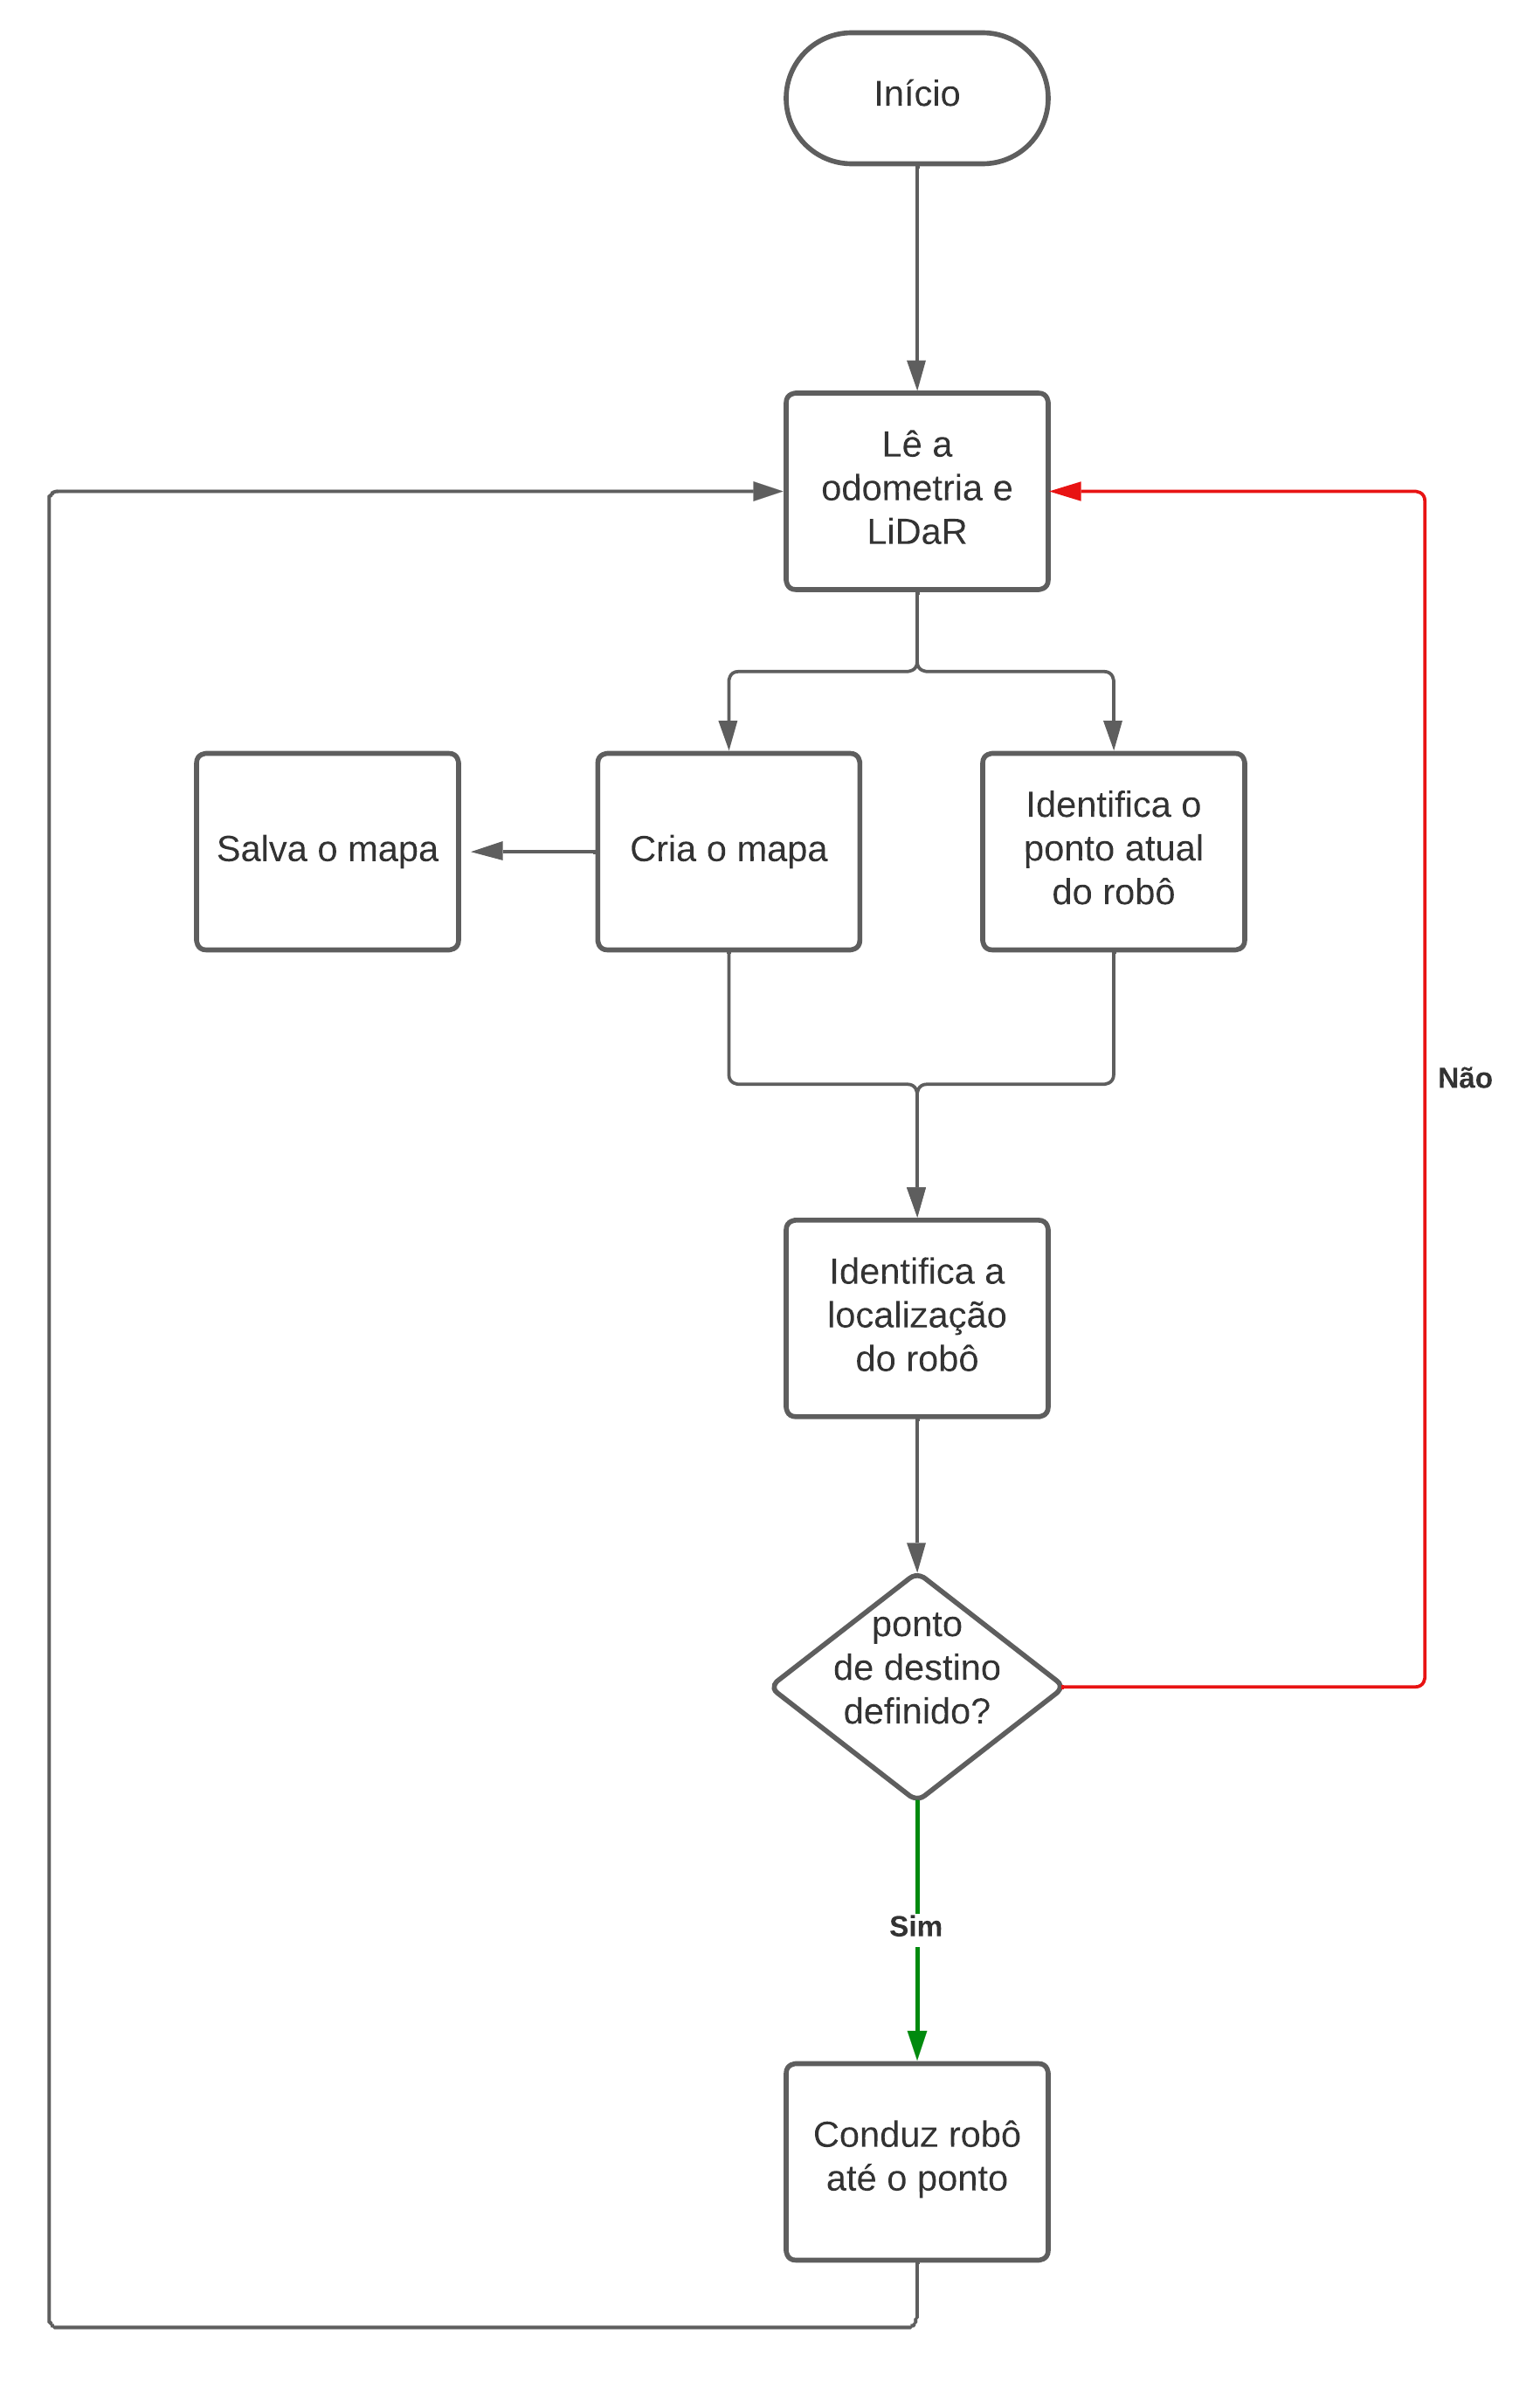
\includegraphics[scale=0.5]{fluxogramaComando.png}
   
    \caption*{Fonte: Autora (2023).}
    \label{fig:fluxogramaComando}
\end{figure}

\subsection{Sistema Operacional de Robô}

Visto a quantidade de singularidades, foi utilizado o ROS para integrar todos os componentes e conectá-los entre o robô e a simulação. Para isso, foram definidas as características do robô em termos que o ROS reconheça, por URDFs (formato de descrição de robô universal) traduzidos dos SDFs para a simulação. Essas descrições foram integradas com informações específicas dos sensores e odometria do robô, para serem acessadas pelas demais bibliotecas e o algoritmo de vagar.

O ROS é constituído por componentes (nomeados como nós) que se comunicam entre si por linhas de comunicação (tópicos) que podem ser acessadas para enviar novas informações (publicar) ou captar informações publicadas (inscrever) por outros nós. Para que essas comunicações entre os nós se tornem mais confiáveis e robustas, foram utilizadas as configurações de qualidade de serviço  a partir do \textit{middleware} Cyclone \cite{qos, cyclone}.

Por fim, a estrutura do modelo proposto é composta pelo robô e o ambiente configurados por arquivos que descrevem todas as suas características importantes. Através do ROS e seu \textit{middleware}, as informações do ambiente simulado são capturadas pelos sensores e são comunicados para as bibliotecas de SLAM e navegação, além do algoritmo de vagar sem colisão. Assim como, os comandos necessários para o robô se mover são repassados pelo intermédio do sistema operacional de robô.

Na Figura~\ref{fig:diagramaBlocosDetalhado}, é encontrada a integração entre todos os componentes supracitados. Em azul, estão as leituras realizadas pelo sensor LiDaR para percepção do ambiente e identificação de obstáculos. Também é representada a odometria, em rosa, coletada pelas informações das rodas. Ambos dados são utilizados pela biblioteca Slam Toolbox e o algoritmo de vagar sem colisões, pelo intermédio do ROS. Assim como, em verde, a velocidade nas rodas é inferida através da definição de seu valor pelo algoritmo de vagar sem colisão ou pela biblioteca Nav2.

\begin{figure}[h]
    \centering
    \caption{Diagrama da integração dos componentes do AtmosBot}
    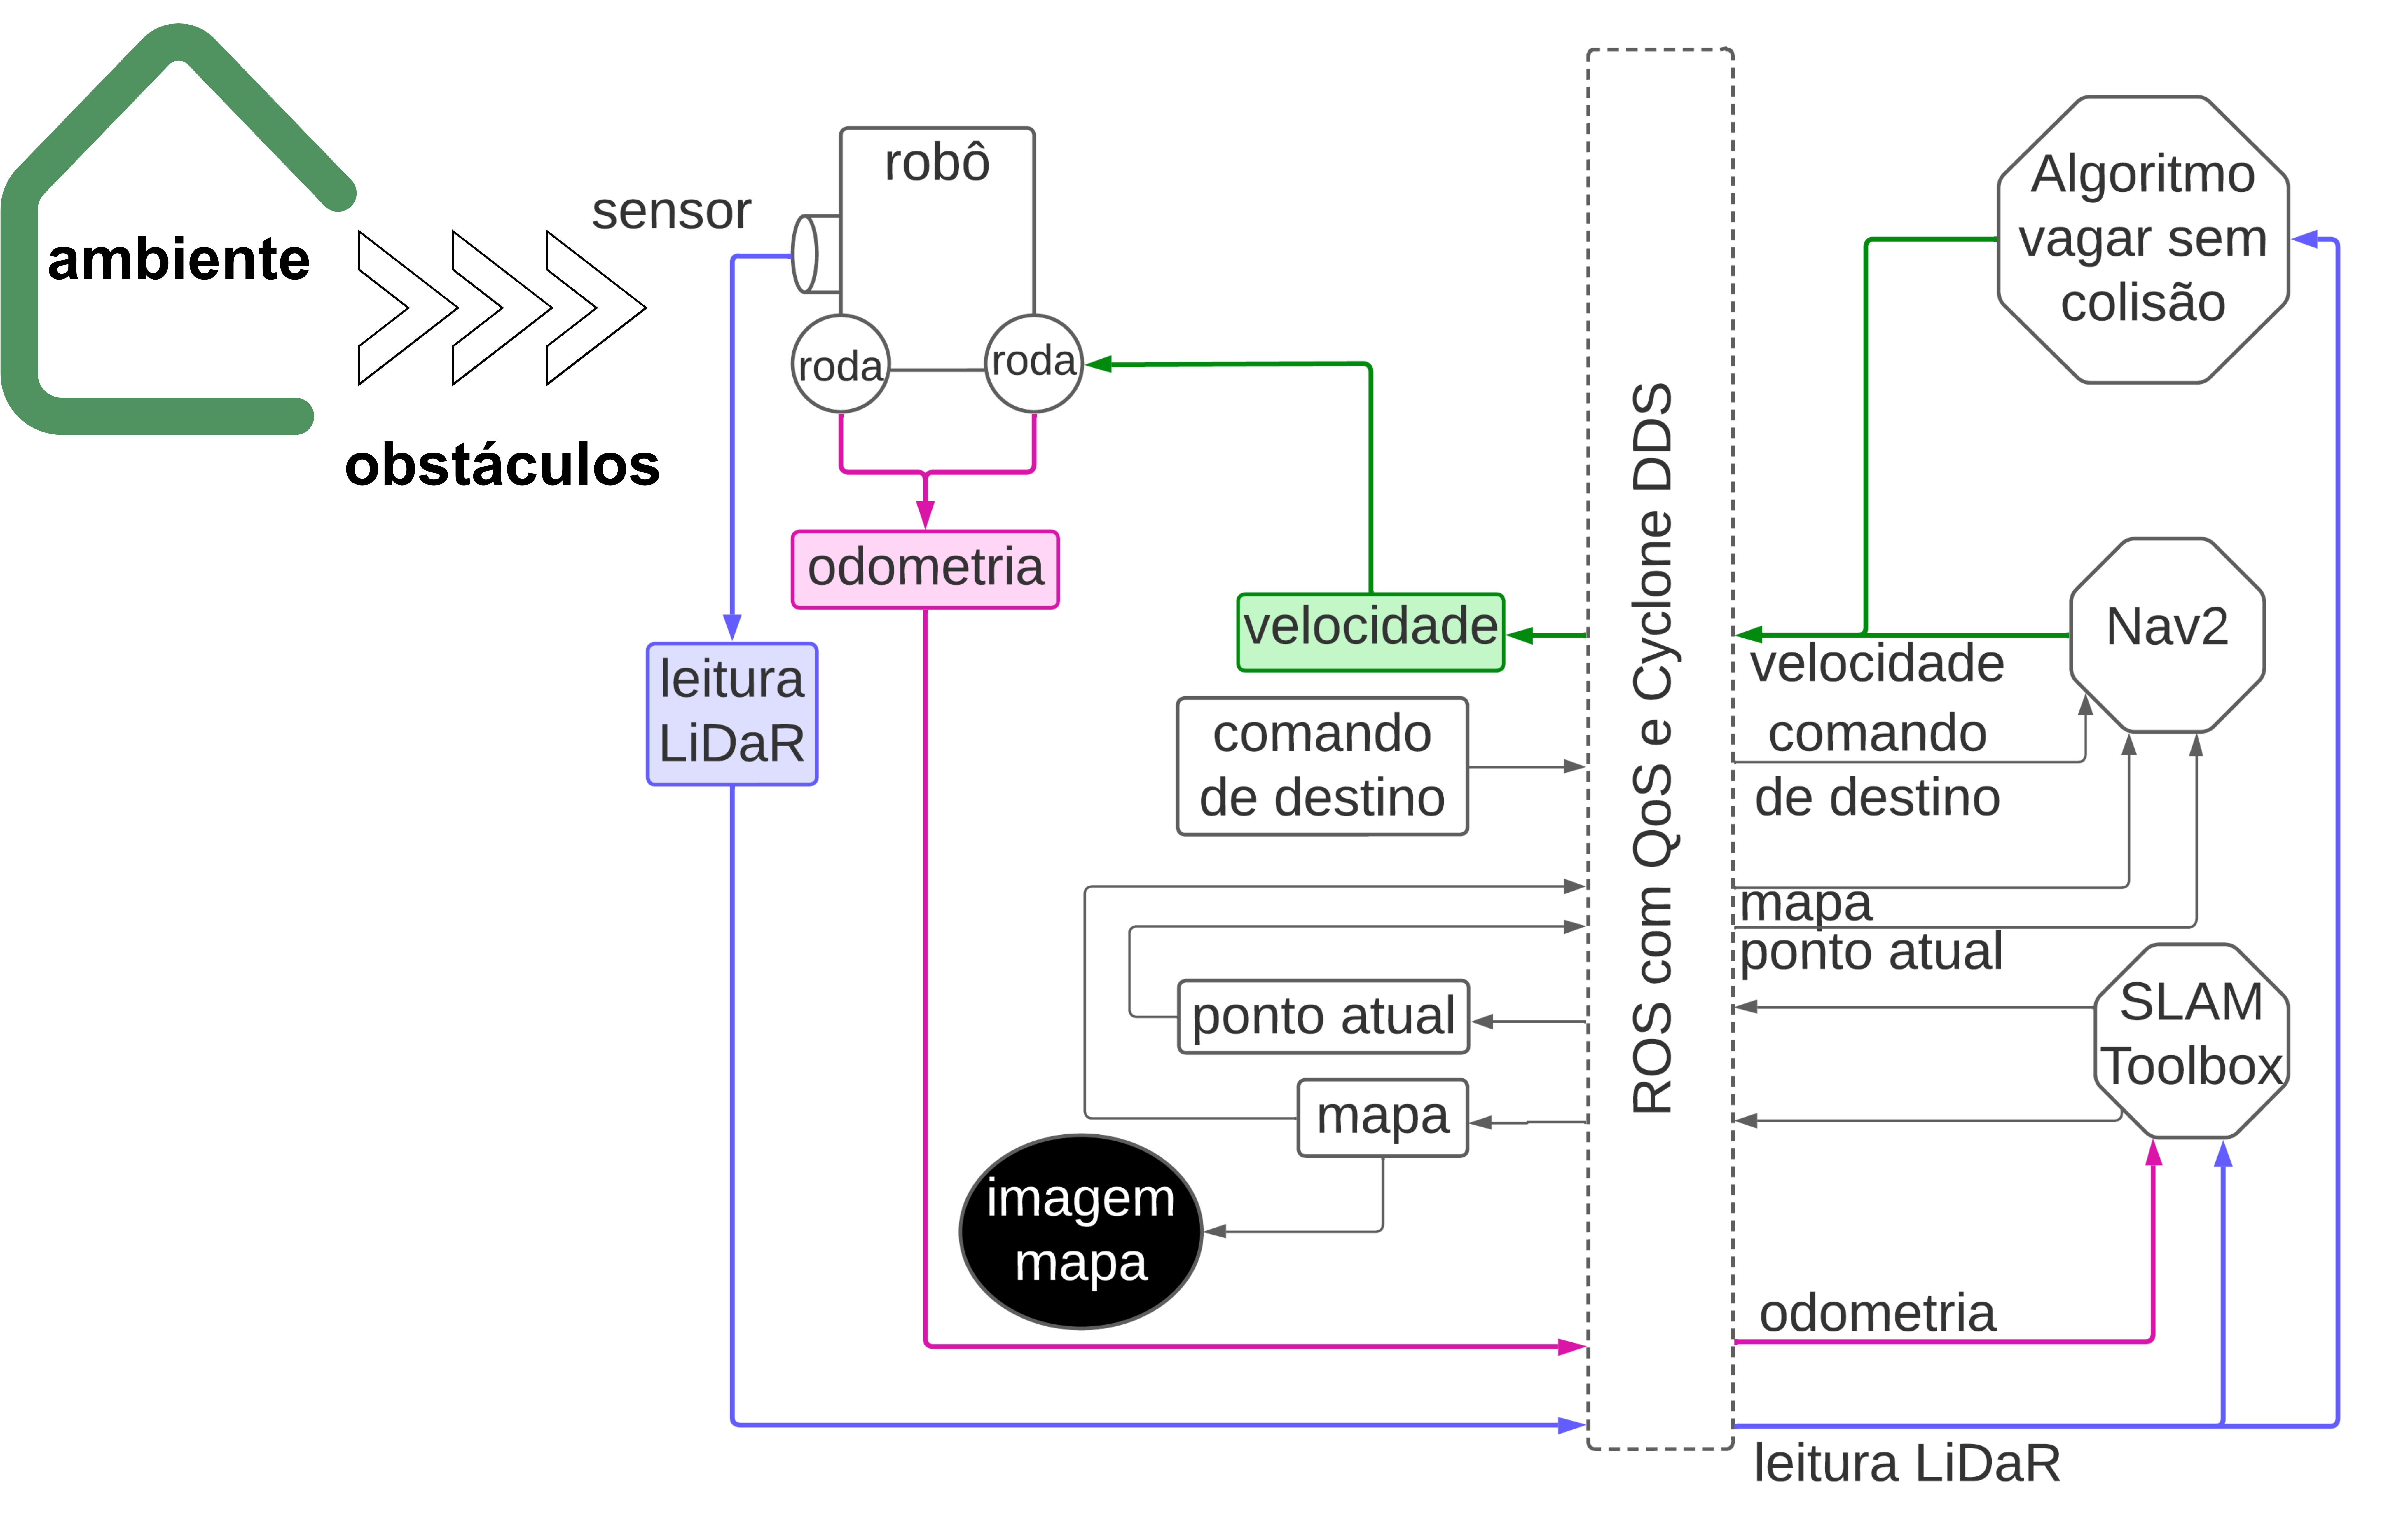
\includegraphics[scale=0.6]{diagramaBlocosDetalhado.png}
    
    \caption*{Fonte: Autora (2023).}
    \label{fig:diagramaBlocosDetalhado}
\end{figure}

\chapter{Resultados e Discussão}
\label{cap-resultadosdiscussao}
A utilização da metodologia detalhada no \chapterautorefname~\ref{cap-metodologia} em conjunto com a implementação da proposta definida no \chapterautorefname~\ref{cap-desenvolvimento},  permitiu o desenvolvimento de um robô simulado capaz de explorar um ambiente desconhecido. Neste capítulo, é exposto e discutido os resultados obtidos com a implementação da solução para o problema norteante deste trabalho. 

\section{Modelo Proposto}
O modelo proposto é constituído por três segmentos: i) a simulação; ii) controle lógico e iii) integração dos componentes. Em seguida, são expostos os resultados obtidos no desenvolvimento de cada segmento.

A estrutura física simulada do robô do presente trabalho foi baseado no modelo disponibilizado por \citet{modeloRobo}. O AtmosBot (Figura~\ref{fig:fotoRobo}) apresenta uma base  tridimensional com quatro rodas comuns e um sensor LiDaR acoplados a ela. Ademais, foi incrementado uma estrutura horizontal  tridimensional com bordas arredondadas e altura de 0,6 metros, no intuito de ser utilizada futuramente como suporte para os instrumentos de localização e manipulação de objetos.

\begin{figure}[h]
    \centering
    \caption{Estrutura física do AtmosBot}
    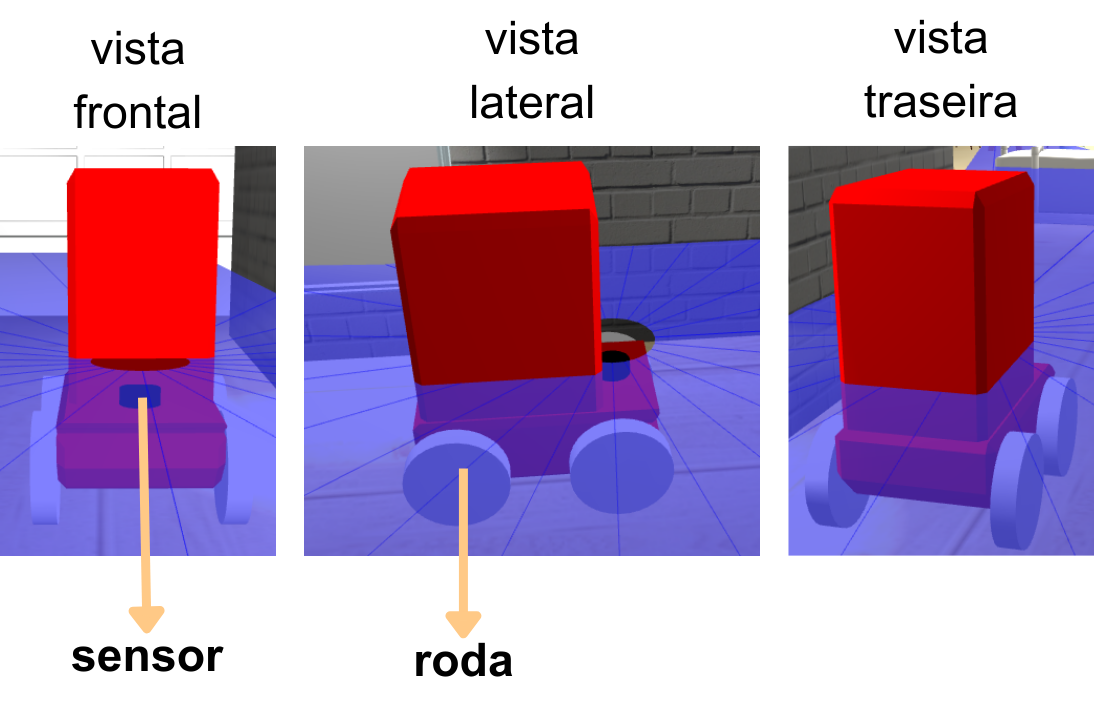
\includegraphics[scale=0.5]{robo.png}
    \caption*{Fonte: Autora (2023).}
    \label{fig:fotoRobo}
\end{figure}

As rodas e o sensor são elementos separados que se integram com a estrutura base do robô a partir das articulações demonstradas na Figura~\ref{fig:roboArticulacoes}. Para as rodas, nos arquivos de descrição de robôs, foi especificado que suas articulações são móveis com o movimento de revolução. Entretanto, para a articulação do sensor, foi definida para se manter estática, a fim de evitar qualquer movimentação indesejada.

\begin{figure}[H]
    \centering
    \caption{Diagrama de articulações do AtmosBot}
    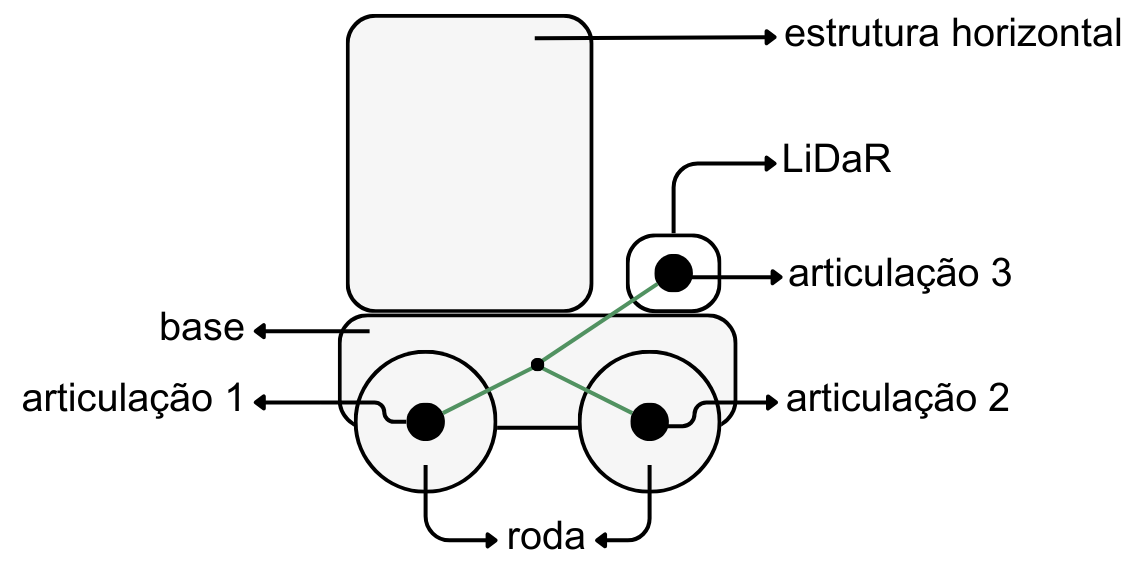
\includegraphics[scale=0.4]{articulacoes.png}
    \caption*{Fonte: Autora (2023).}
    \label{fig:roboArticulacoes}
\end{figure}

O controle lógico do robô está diretamente conectada com a sua navegação autônoma. Os módulos que controlam o robô, para ele se movimentar autonomamente sem colidir com os obstáculos, utilizam as informações do ambiente captadas pelo sensor LiDaR. Na parte superior da Figura~\ref{fig:visaoLidar}, é possível visualizar os feixes de luz do sensor, representados pelas linhas azuis, no simulador Gazebo. Esse sensor atua na horizontal, contendo 24 raios com uma distância de 15 graus entre eles e um alcance de 3,5 metros. Cada feixe capta a distância, em metros, do seu ponto de origem até o obstáculo à sua frente que reflete as ondas óticas. Foi utilizado o valor mínimo entre as distâncias captadas no intervalo de 90 graus em cada extremidade, para identificar os pontos com obstáculos mais próximos nas laterais. Pelo programa RVIZ, na parte inferior da Figura~\ref{fig:visaoLidar}, as capturas do LiDaR são expostas em esferas vermelhas.

\begin{figure}[H]
    \centering
    \caption{Capturas do sensor LiDaR}
    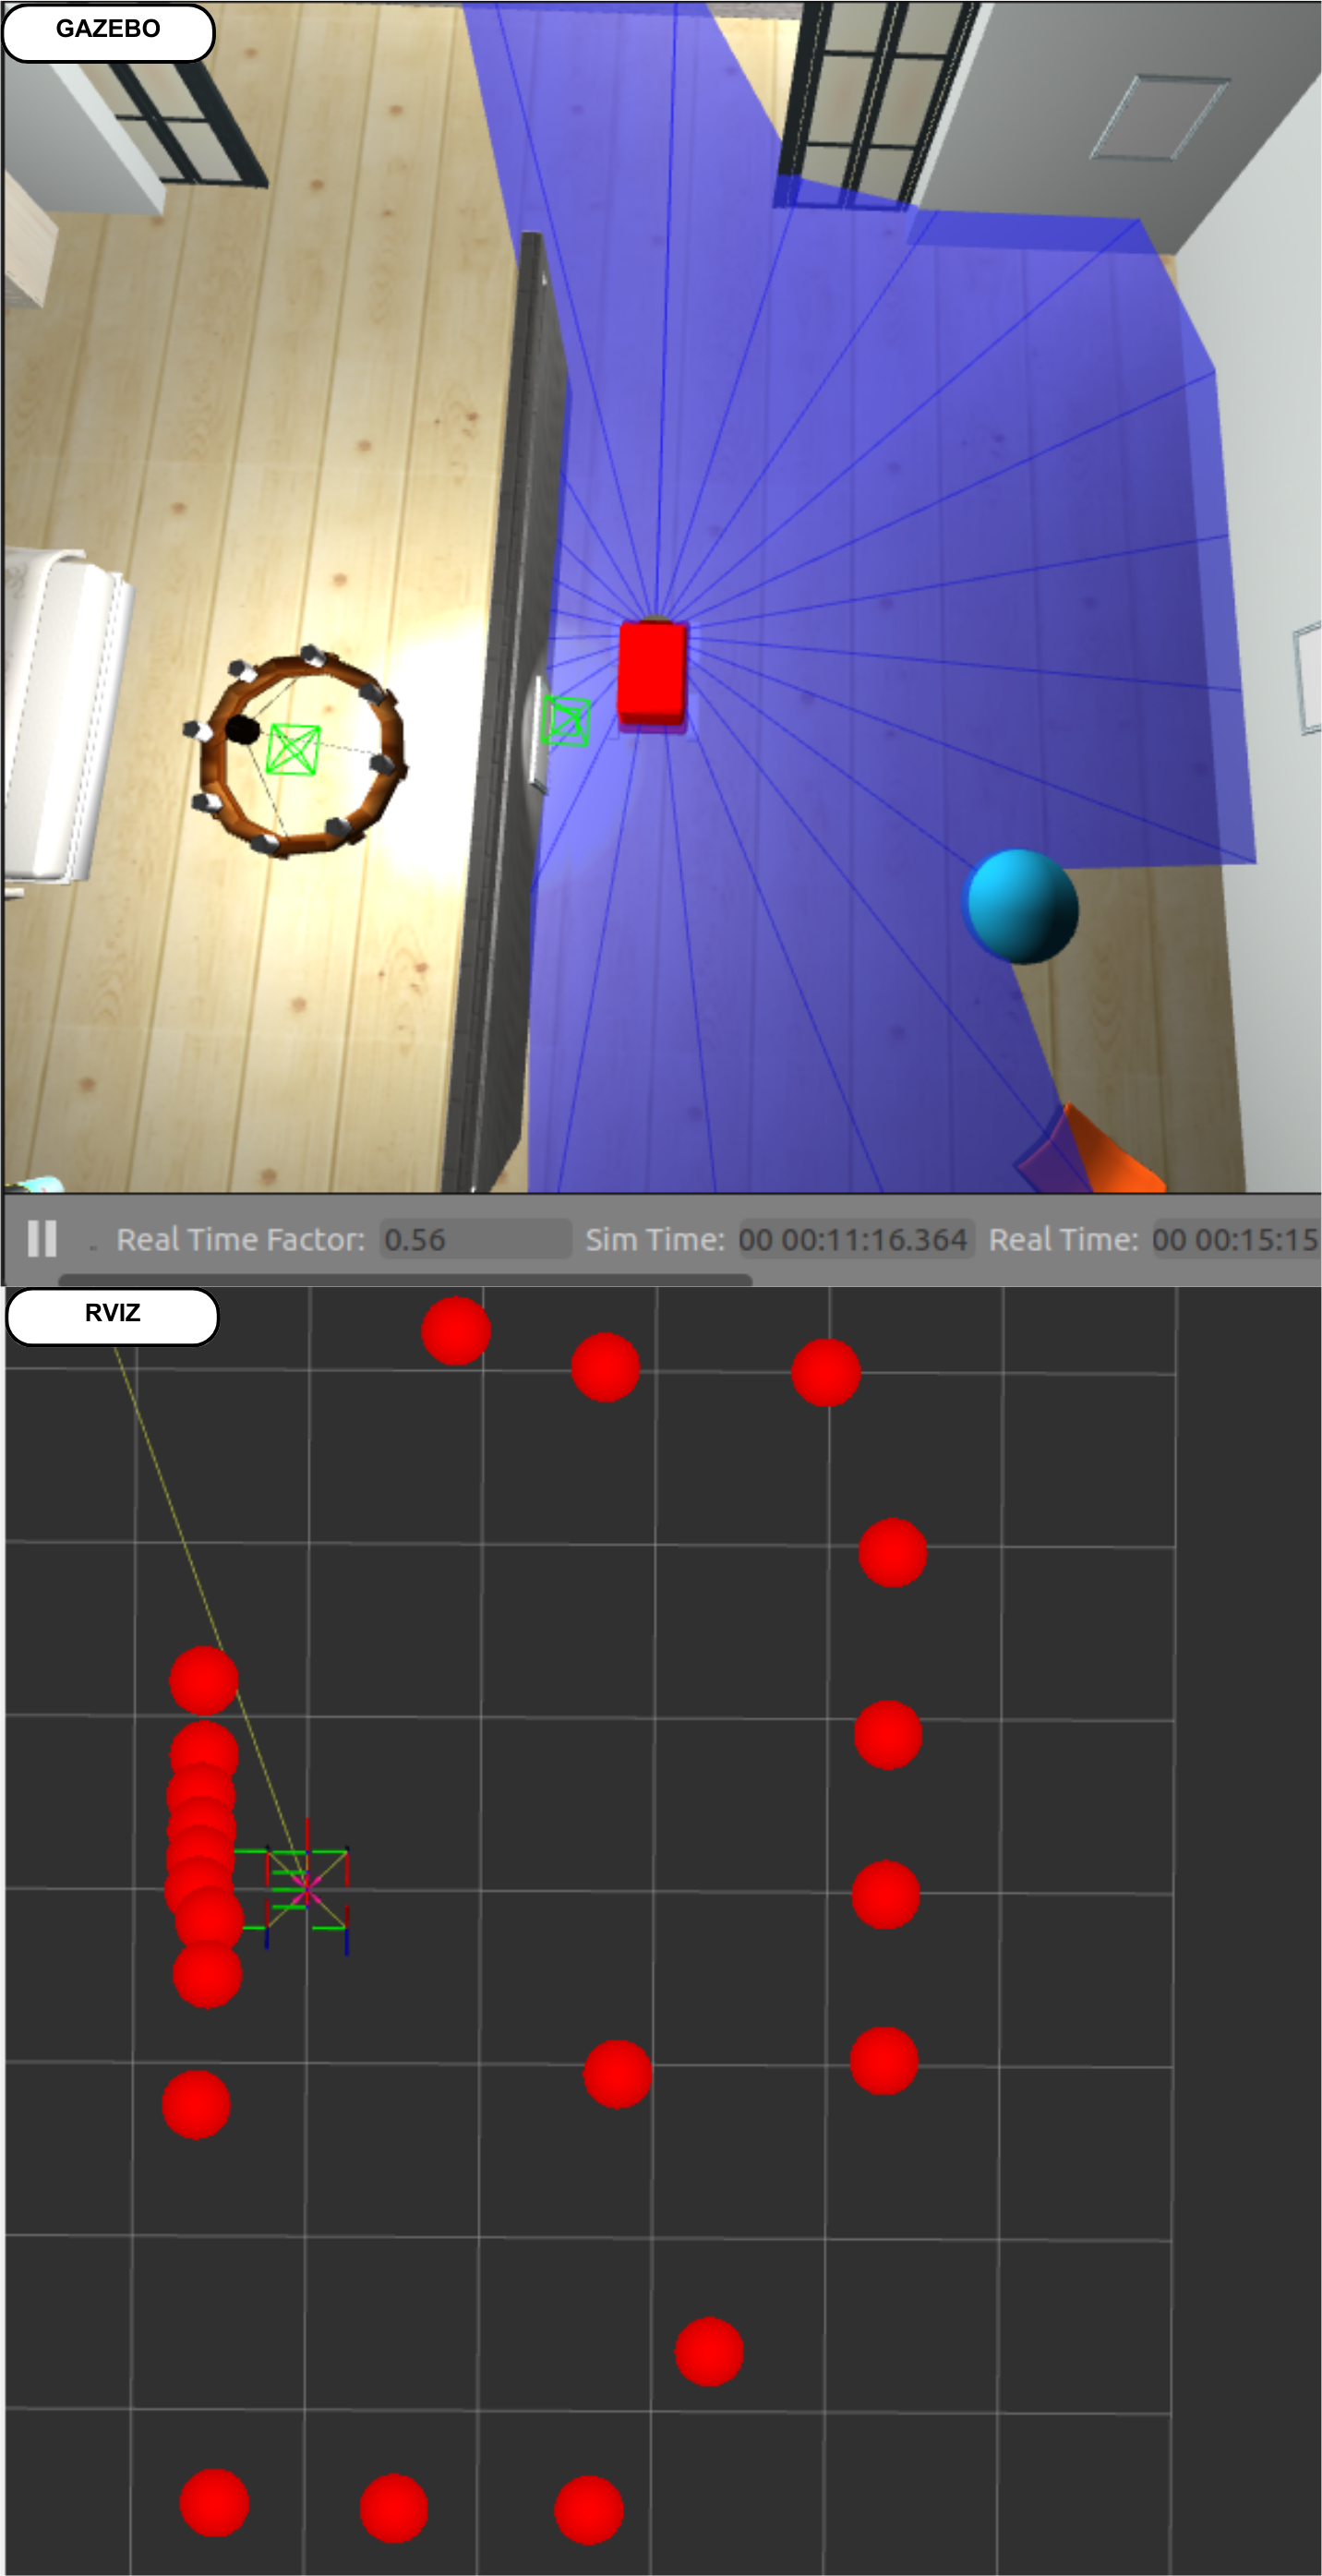
\includegraphics[scale=0.25]{laser.png}
    \caption*{Fonte: Autora (2023).}
    \label{fig:visaoLidar}
\end{figure}

Neste trabalho, o sensor LiDaR permitiu a detecção de obstáculos para que o AtmosBot conseguisse navegar com o mínimo de colisões. Segundo \citet{dpoom}, a câmera RGB com profundidade também é um instrumento muito utilizado para a detecção de obstáculos, podendo ser considerada um recurso mais barato. Entretanto, \citet{navegacaoSlam:2022} identifica que existe um custo maior no processamento das informações de profundidade disponibilizadas por tais câmeras. Por outro lado, como comprovado por \citet{navegacaoSlam:2022}, o sensor LiDaR  alcança o mesmo objetivo de detectar obstáculos durante a navegação do robô de forma satisfatória, com menor custo computacional. Além disso, os resultados obtidos da pesquisa bibliográfica para instrumentos de percepção do ambiente (Figura~\ref{fig:graficoPesquisaPercepcao}) revelam uma maior porcentagem de utilização do sensor LiDaR em trabalhos correlatos. Portanto, visto seu menor custo de processamento, capacidade similar de detecção de obstáculos e alta relevância, é mais coerente e vantajoso utilizar o LiDaR no cenário da problemática deste trabalho. 

Ao longo da exploração do ambiente pelo AtmosBot, o módulo Slam Toolbox cria (e atualiza) um mapa com as informações capturadas pelo LiDaR e pela odometria. Esse mapa é constituído por \textit{pixels} brancos, que correspondem a áreas livres, e pretos, equivalentes aos obstáculos. Pelo programa RVIZ é possível visualizar o mapa sendo criado, como disposto na parte inferior da Figura~\ref{fig:mapaRviz}, conforme os obstáculos presentes na simulação, representada na parte superior da Figura~\ref{fig:mapaRviz}.

\begin{figure}[H]
    \centering
    \caption{Mapa em criação pelo Slam Toolbox}
    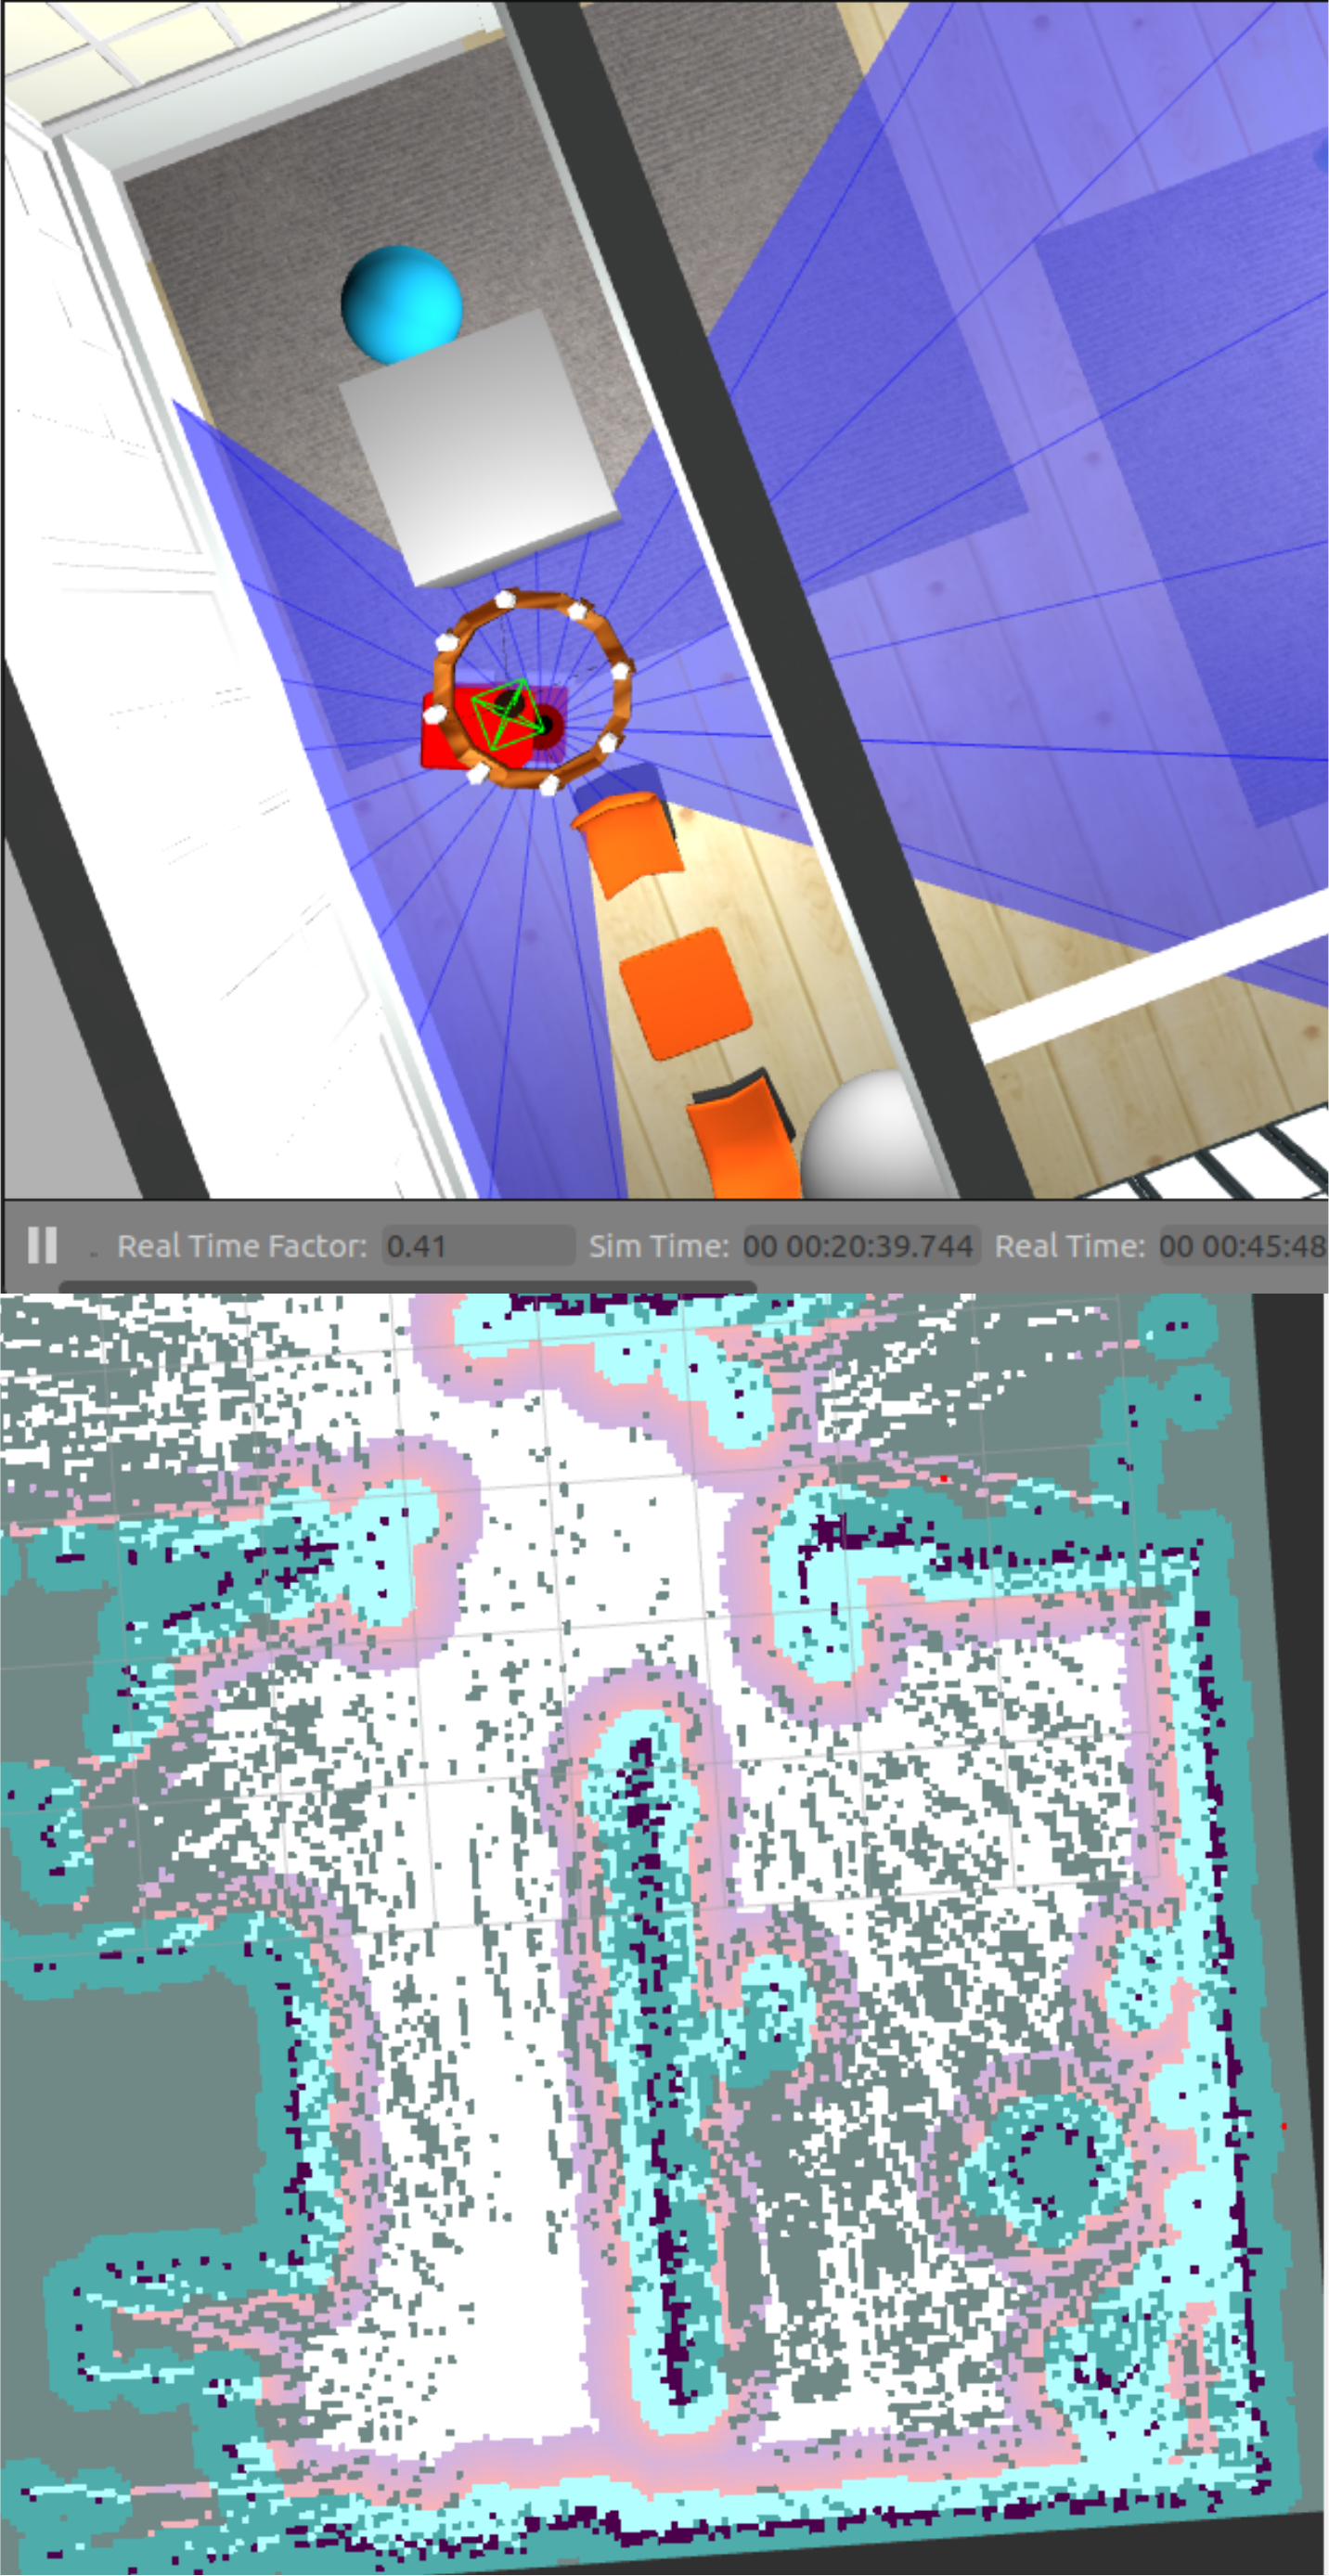
\includegraphics[scale=0.2]{mapRVIZ.png}
    \caption*{Fonte: Autora (2023).}
    \label{fig:mapaRviz}
\end{figure}

No momento de execução, além do mapa de obstáculos e áreas livres, é criado em tempo real um mapa temporário com as áreas de colisão, nomeado como mapa de custos. Nesse formato de mapa, são definidos pesos (custos) para cada área do ambiente, definindo valores maiores para áreas ocupadas por obstáculos e valores intermediários para um raio ao redor dos elementos a serem evitados. Na parte inferior da Figura~\ref{fig:costmap}. estão expostos os obstáculos presentes na simulação (na parte superior da figura). A cor roxa representa uma área perigosa, próxima a um obstáculo. O vermelho indica uma área de colisão com algum elemento do ambiente. Por fim, em azul são representados o centro de massa dos obstáculos.

\begin{figure}[H]
    \centering
    \caption{Mapa de custos temporário}
    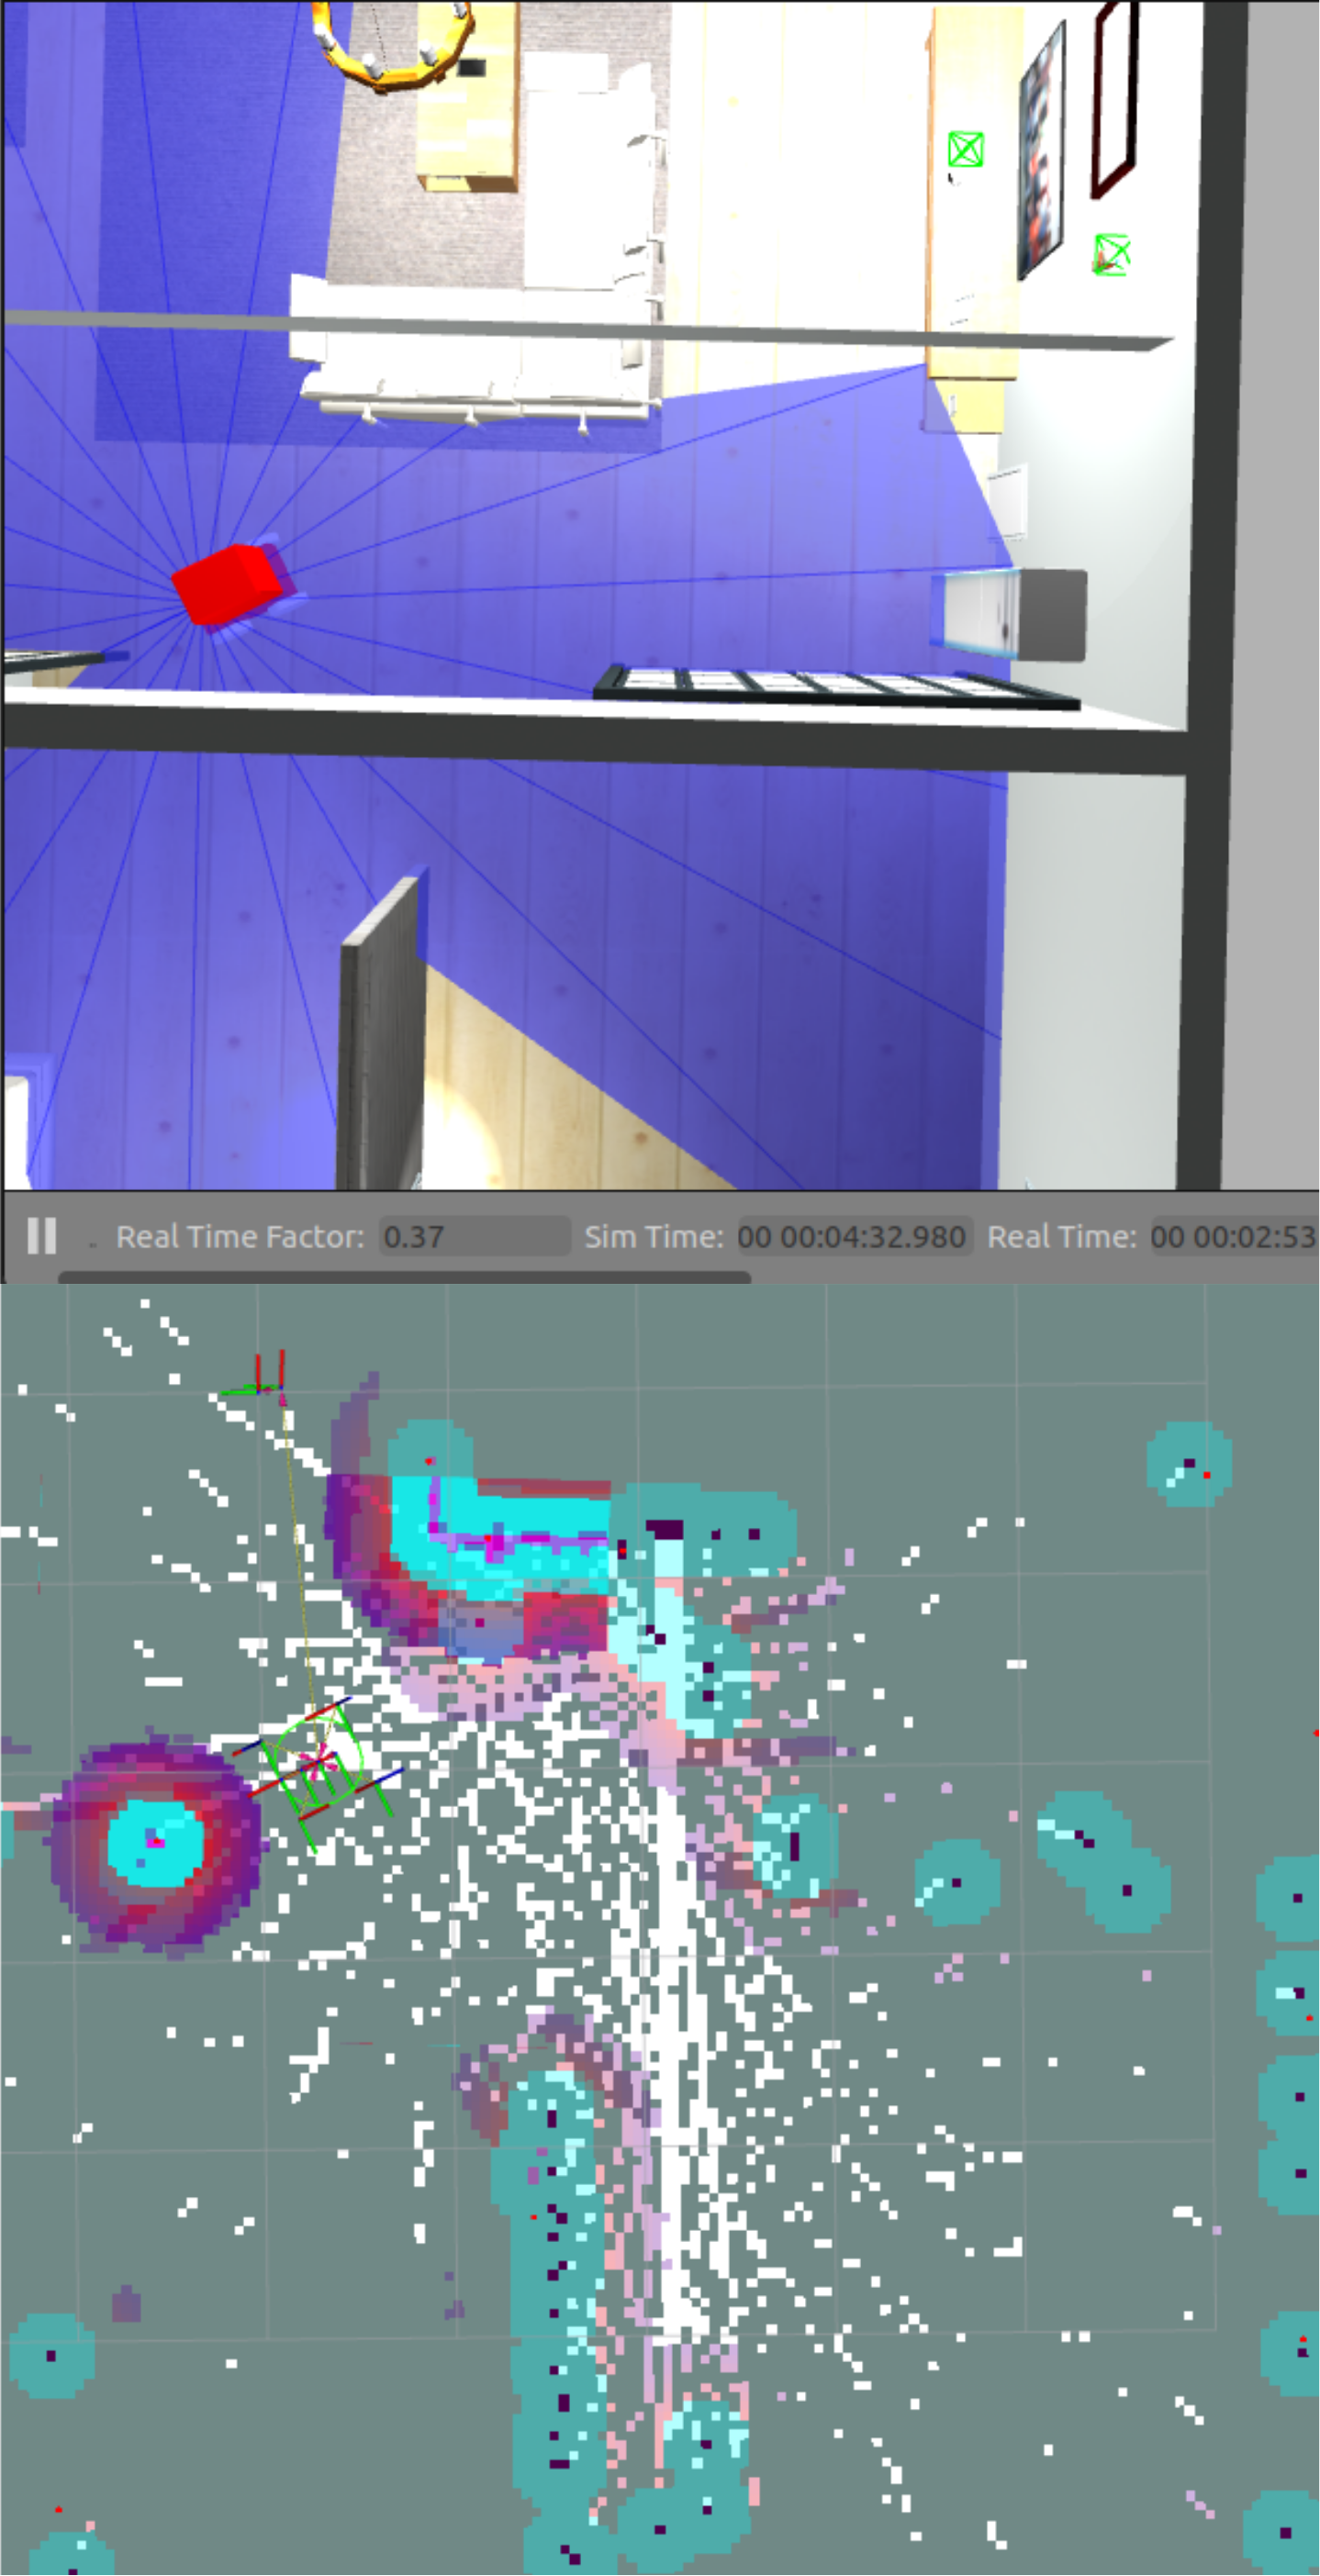
\includegraphics[scale=0.26]{costmap.png}
    \caption*{Fonte: Autora (2023).}
    \label{fig:costmap}
\end{figure}

Com o ambiente completamente, ou parcialmente, explorado, a biblioteca Slam Toolbox permite salvar o mapa de obstáculos, criado com a navegação autônoma, em formato de imagem (Figura~\ref{fig:mapaImagem}) ou serializado. Como o ambiente em que o AtmosBot atua é desconhecido, o seu mapeamento é realizado durante a sua exploração conforme as informações do sensor LiDaR. Em \citet{navegacaoSlam:2022} o ambiente foi mapeado pelo robô controlado remotamente para, em seguida, iniciar sua navegação autônoma com o mapa criado. Essa abordagem resultou em uma divergência de 0,2 metros entre o modelo produzido e a realidade. Assim, para não encontrar essas diferenças, é mais vantajoso mapear o ambiente autonomamente enquanto o robô explora o meio e evitar colisões a partir das capturas do LiDaR. Além disso, como visto, o Slam Toolbox fornece a possibilidade de atualizar o mapa que será utilizado para a localização do robô por outros módulos. 


\begin{figure}[H]
    \centering
    \caption{Imagem do mapa criado pela exploração}
    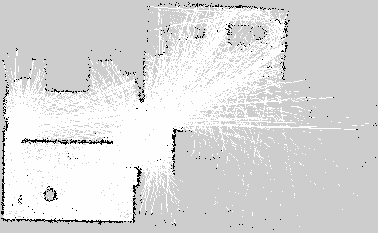
\includegraphics[scale=1]{saved_map.png}
    \caption*{Fonte: Autora (2023).}
    \label{fig:mapaImagem}
\end{figure}


O mapa de áreas livres disponibilizado pelo módulo Slam Toolbox é acessado pela biblioteca Nav2. Com o mapa e a posição atual do robô, é possível identificar a sua localização no ambiente. Pelo programa RVIZ é possível emitir uma instrução para o robô, definindo um ponto de destino. O módulo Nav2 oferece o suporte para realizar a navegação até o objetivo definido de forma autônoma sem colidir com os obstáculos identificados ao longo do caminho. Na Figura~\ref{fig:trajetoriaNav2}, está destacada a trajetória definida para o ponto de destino, representada como uma linha vermelha, conforme o comando inserido no RVIZ.


\begin{figure}[H]
    \centering
    \caption{Trajetória elaborada pelo Nav2}
    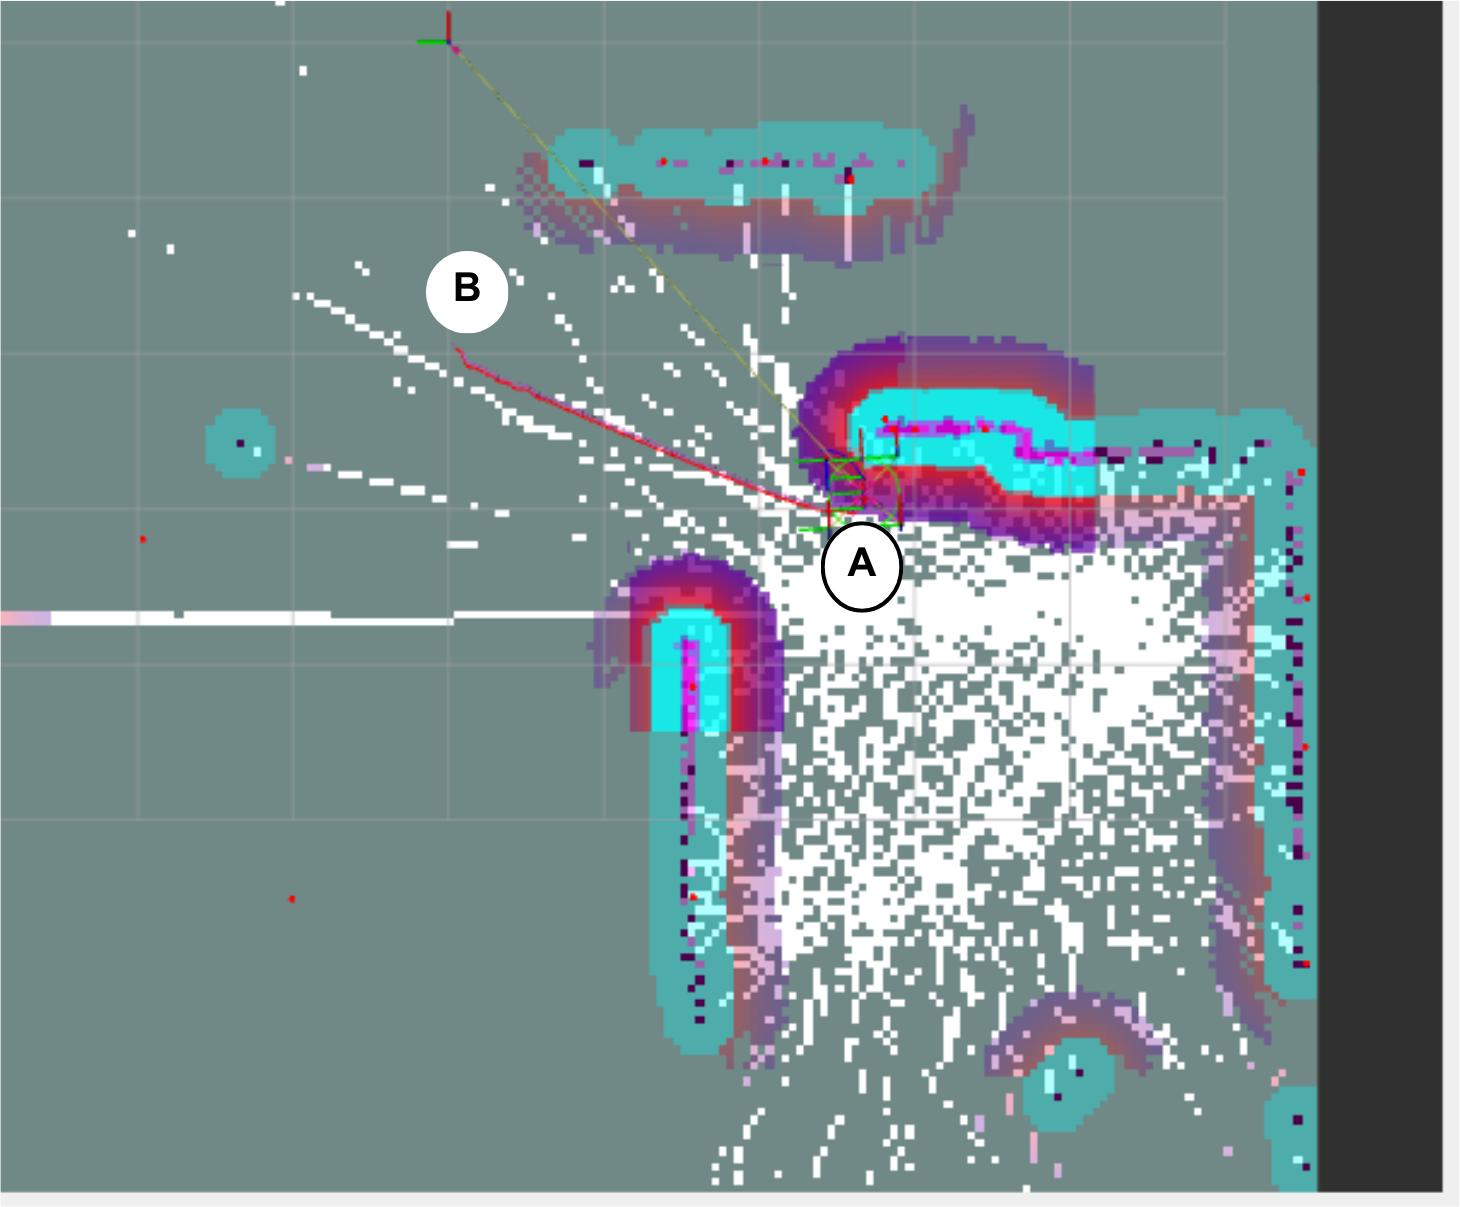
\includegraphics[scale=0.4]{trajetoria.png}
    \caption*{Fonte: Autora (2023).}
    \label{fig:trajetoriaNav2}
\end{figure}

As sub-tarefas do robô se complementam para que ele seja capaz de navegar autonomamente por um ambiente desconhecido. Foi desnecessária a implementação de um algoritmo específico para a localização do robô, como feito por \citet{navegacaoSlam:2022} com o algoritmo AMCL e por \citet{dpoom} com o aprendizado profundo reforçado. Pois, com a integração das bibliotecas Nav2 e Salm Toolbox, foi obtida essa funcionalidade de localização do robô com a dispensa de maiores incrementos.

Por fim, a implementação do Sistema Operacional de Robô (ROS) permitiu a integração entre todos os módulos e a simulação. O ROS realizou o papel crucial de intermédio entre todos os elementos do robô, permitindo que a mesma proposta possa ser utilizada além da simulação sem mudanças drásticas, como demonstrado por \citet{navegacaoSlam:2022, dpoom, lidarRGBD}.

\section{Ambiente Simulado}
O robô autônomo móvel modelado tem o objetivo de navegar de forma autônoma em um domicílio. Dito isso, o ambiente simulado foi montado para ter grande semelhança com uma residência. Para o presente trabalho é considerado como uma casa qualquer ambiente interno que contenha espaços definidos de convivência, com no mínimo um dormitório e uma cozinha. Com a ferramenta da AWS, foi possível simular um domicílio com três espaços diferentes: um dormitório, uma sala de estar e uma cozinha. Esses espaços não são divididos por paredes ou portas, possibilitando o acesso completo à casa. Cada espaço comporta elementos típicos, como cama, sofá, mesa, geladeiras e balcões. Além disso, também foram disponibilizados outros componentes para enriquecer o cenário, como produtos de academia, quadros e cabeceiras. Na Figura~\ref{fig:ambiente}, é possível visualizar o ambiente elaborado através do simulador Gazebo.

\begin{figure}[H]
    \centering
    \caption{Ambiente elaborado pela plataforma AWS}
    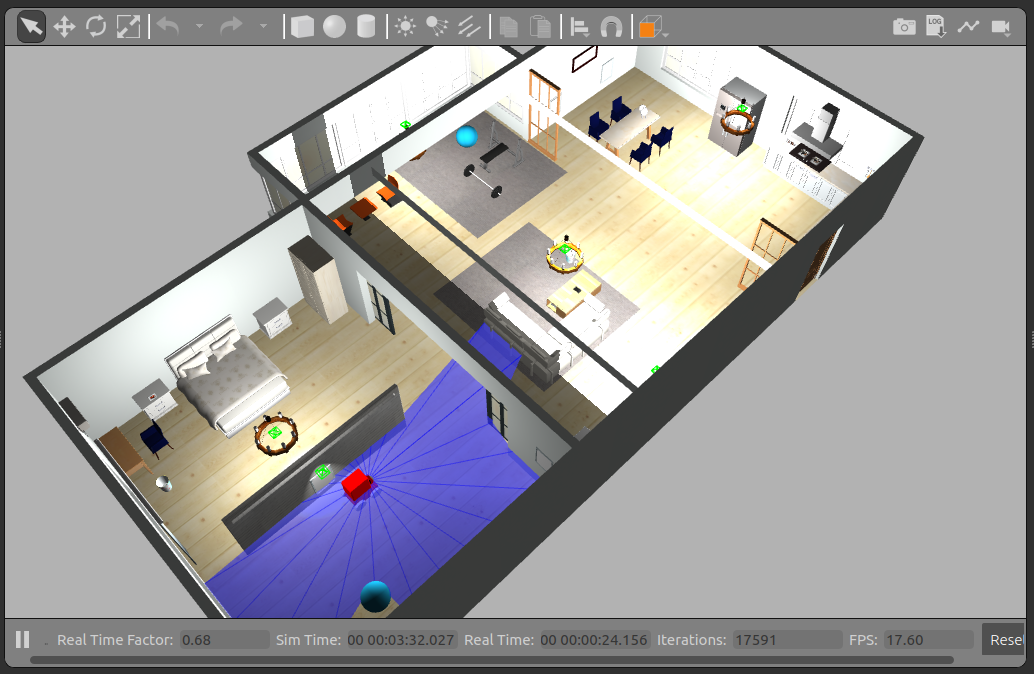
\includegraphics[scale=0.4]{ambiente.png}
    \caption*{Fonte: Autora (2023).}
    \label{fig:ambiente}
\end{figure}

\section{Resultados dos Testes}
Com o modelo proposto finalizado, foi possível validá-lo integralmente com os casos de teste elaborados e definidos no \appendixautorefname~\ref{appendix-casosTeste}. A partir dessa validação, tornou viável analisar quais os requisitos do robô, e do ambiente, foram alcançados pela implementação da solução proposta neste trabalho.

Em cada teste, foi executada a ação detalhada no caso de teste correspondente e o resultado obtido foi registrado no \appendixautorefname~\ref{appendix-resultadosTestes}. Os resultados dos casos de teste permitiram analisar quais requisitos definidos anteriormente foram alcançados com sucesso e validar o modelo completo. Os casos de teste foram elaborados conforme os requisitos levantados no início da especificação do sistema. Esses requisitos foram categorizados por prioridade no desempenho do sistema, sendo essas prioridades: i) essencial; ii) importante; iii) desejável. Com essa categorização, é possível compreender o patamar de funcionamento que o robô se encontra após desenvolvido e validado.

Os requisitos com prioridade essencial fazem parte de um conjunto de especificações que determinam os elementos fundamentais para o modelo ser funcional, sem eles o modelo não pode ser considerado um produto minimamente viável. Esses elementos tratam sobre: i) a movimentação do robô pelo ambiente sem colidir com os obstáculos presentes; ii) as mudanças frequentes que o ambiente precisa ter para representar um domicílio real com morador; iii) a verossimilhança do ambiente simulado com uma residência comum e iv) a inexistência de portas fechadas entre espaços que o robô deveria acessar, além de degraus e escadas. Diante os quatro requisitos citados, com os testes realizados, foi observado que todos eles foram alcançados.

Os requisitos com prioridade importante, são requisitos necessários para um funcionamento adequado do modelo proposto. Entretanto, a sua inexistência não limita esse funcionamento, diferente dos requisitos essenciais. Os requisitos importantes abordam a movimentação e identificação do robô. Os correspondentes testes realizados apontam que foram alcançados os dois requisitos importantes definidos previamente.

Por fim, os requisitos com prioridade desejável representam especificações que tornam ótimo o funcionamento do modelo. Caso esses requisitos não sejam atendidos, o desempenho do modelo não é afetado negativamente. Com isso, é possível serem incrementados apenas em próximas versões. Com os testes realizados, foi identificado todos os requisitos desejáveis foram alcançados.

Os casos de teste sobre a movimentação do robô e a dinamicidade do ambiente (CT01, CT02, CT03, CT04 e CT05) tiveram testes com repetições para obter o sucesso médio dos casos de teste. Os casos de teste referentes são:
\begin{enumerate}
    \item CT01 - detalha às direções possíveis que o robô é capaz de se movimentar, como demonstrado na Figura~\ref{fig:teste1CT01} com a amostra da execução de uma das repetições dos seus testes;
    \item CT02 - capacidade do robô se esquivar dos obstáculos no ambiente, como demonstrado na Figura~\ref{fig:teste1CT02}  com a amostra da execução de uma das repetições dos seus testes;
    \item CT03 - locomoção do robô em diferentes superfícies (como tapete e piso liso), como demonstrado na Figura~\ref{fig:teste1CT03}  com a amostra da execução de uma das repetições dos seus testes;
    \item CT04 - velocidade segura do robô para os seres e propriedade ao seu redor, como demonstrado na Figura~\ref{fig:teste1CT04}  com a amostra da execução de uma das repetições dos seus testes;
    \item CT05 - capacidade de alterar a posição dos elementos da simulação, como demonstrado na Figura~\ref{fig:teste1CT05}  com a amostra da execução de uma das repetições dos seus testes.
\end{enumerate}

\begin{figure}[H]
    \centering
    \caption{Captura da primeira repetição CT01}
    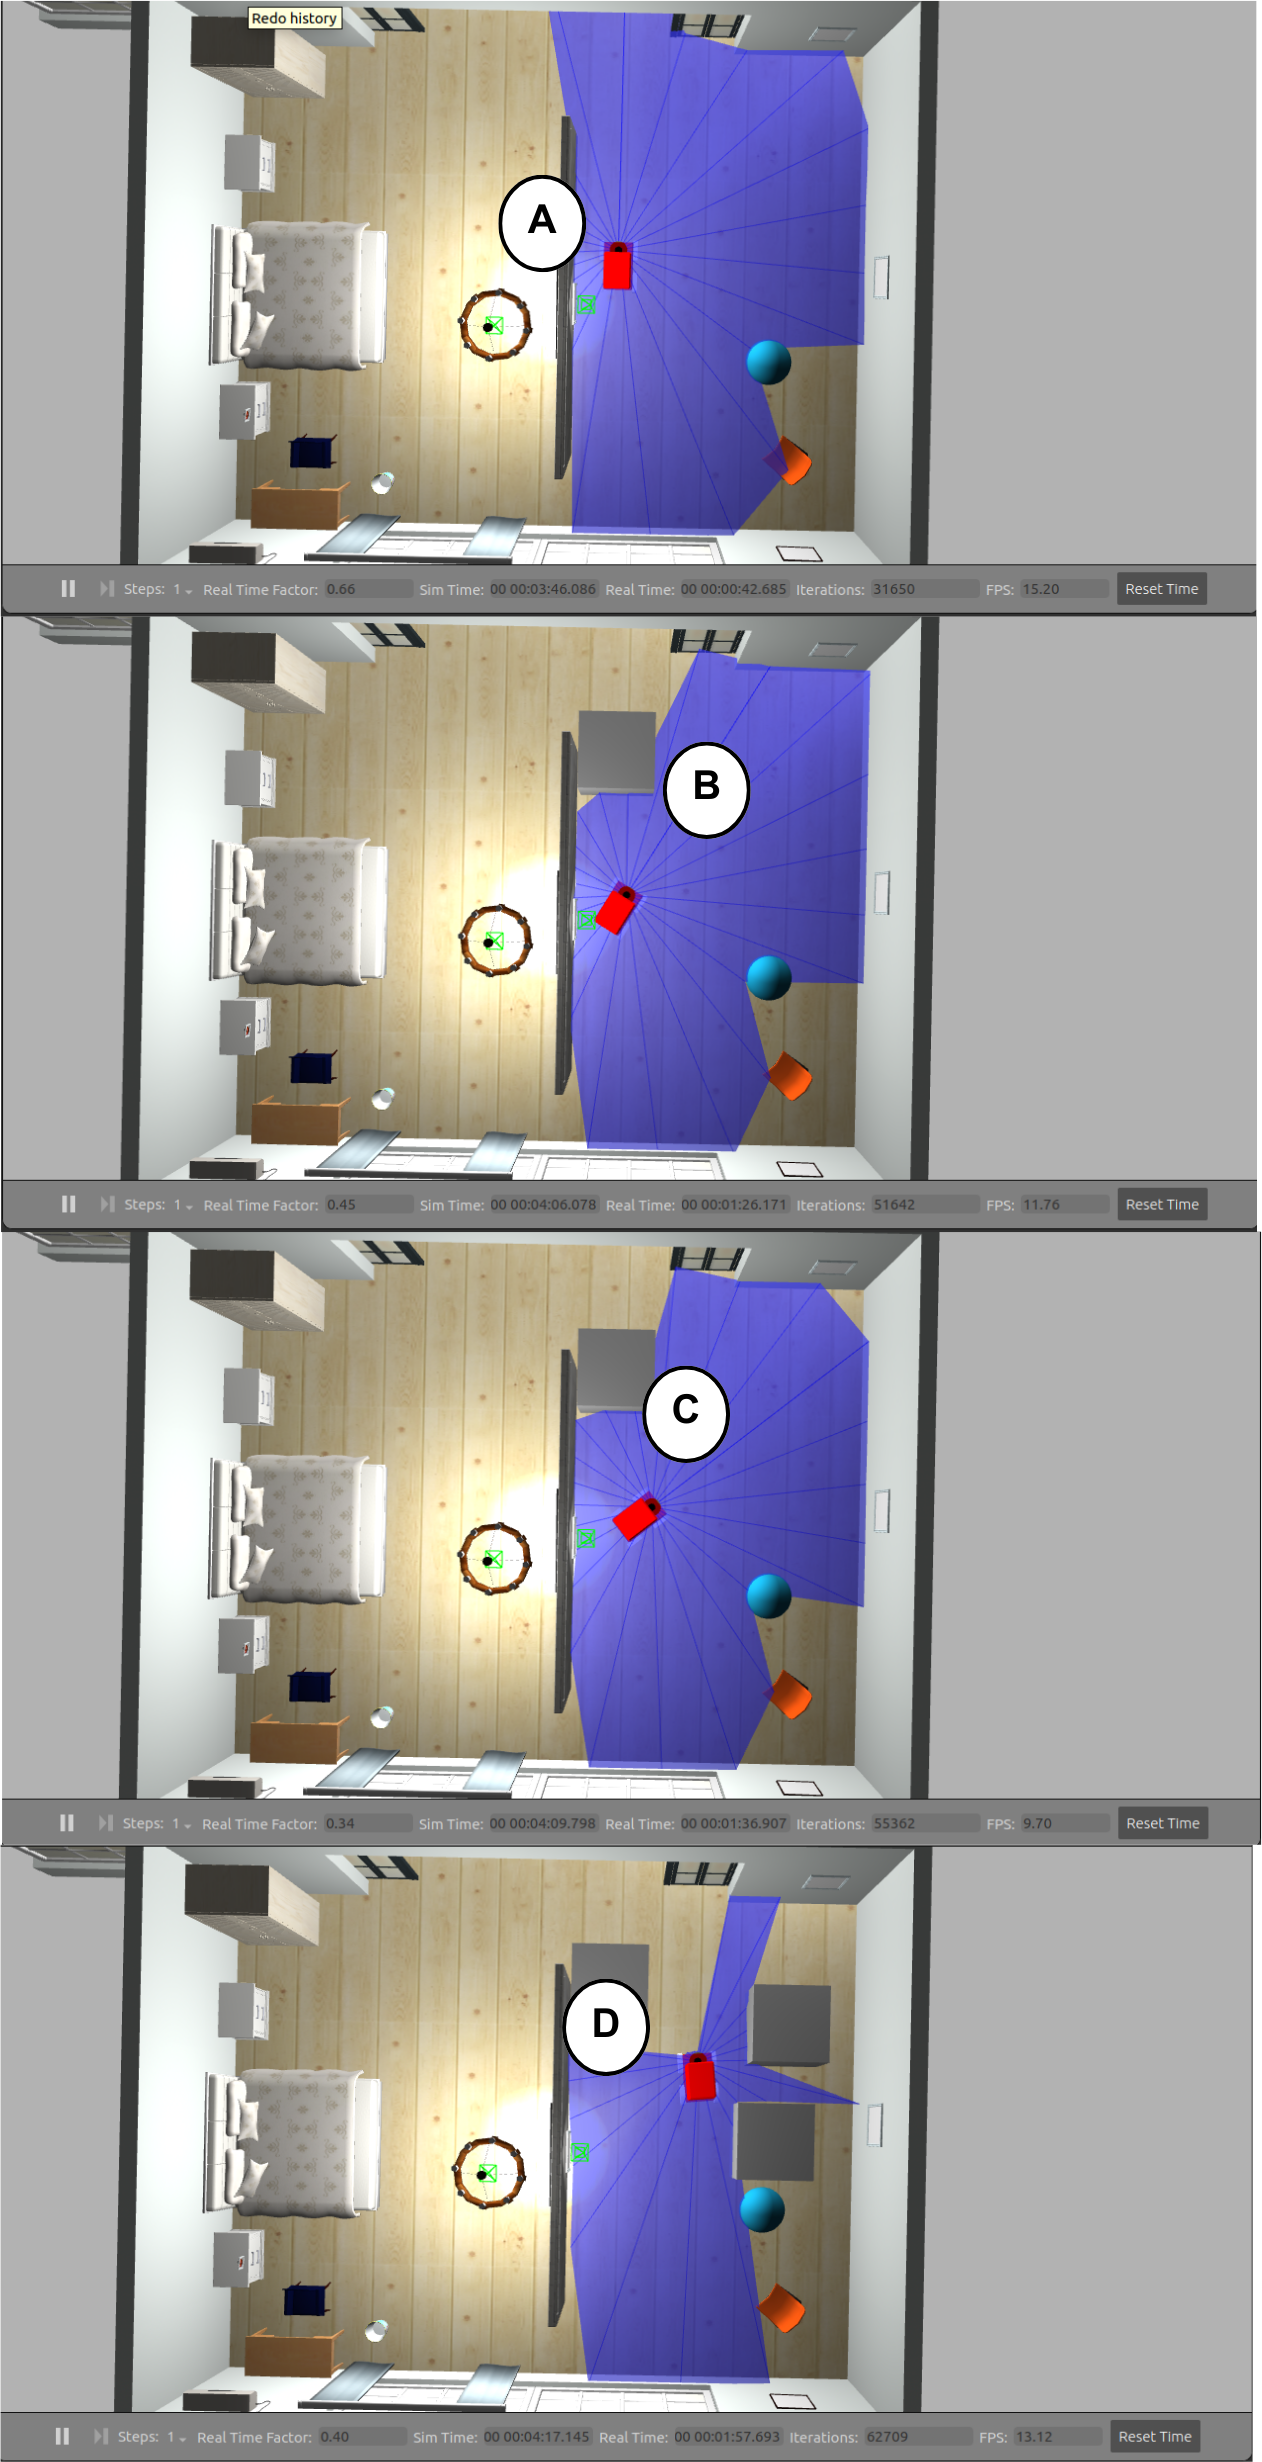
\includegraphics[scale=0.35]{ct01_1.png}
    \caption*{Fonte: Autora (2023).}
    \label{fig:teste1CT01}
\end{figure}

\begin{figure}[H]
    \centering
    \caption{Captura da primeira repetição CT02}
    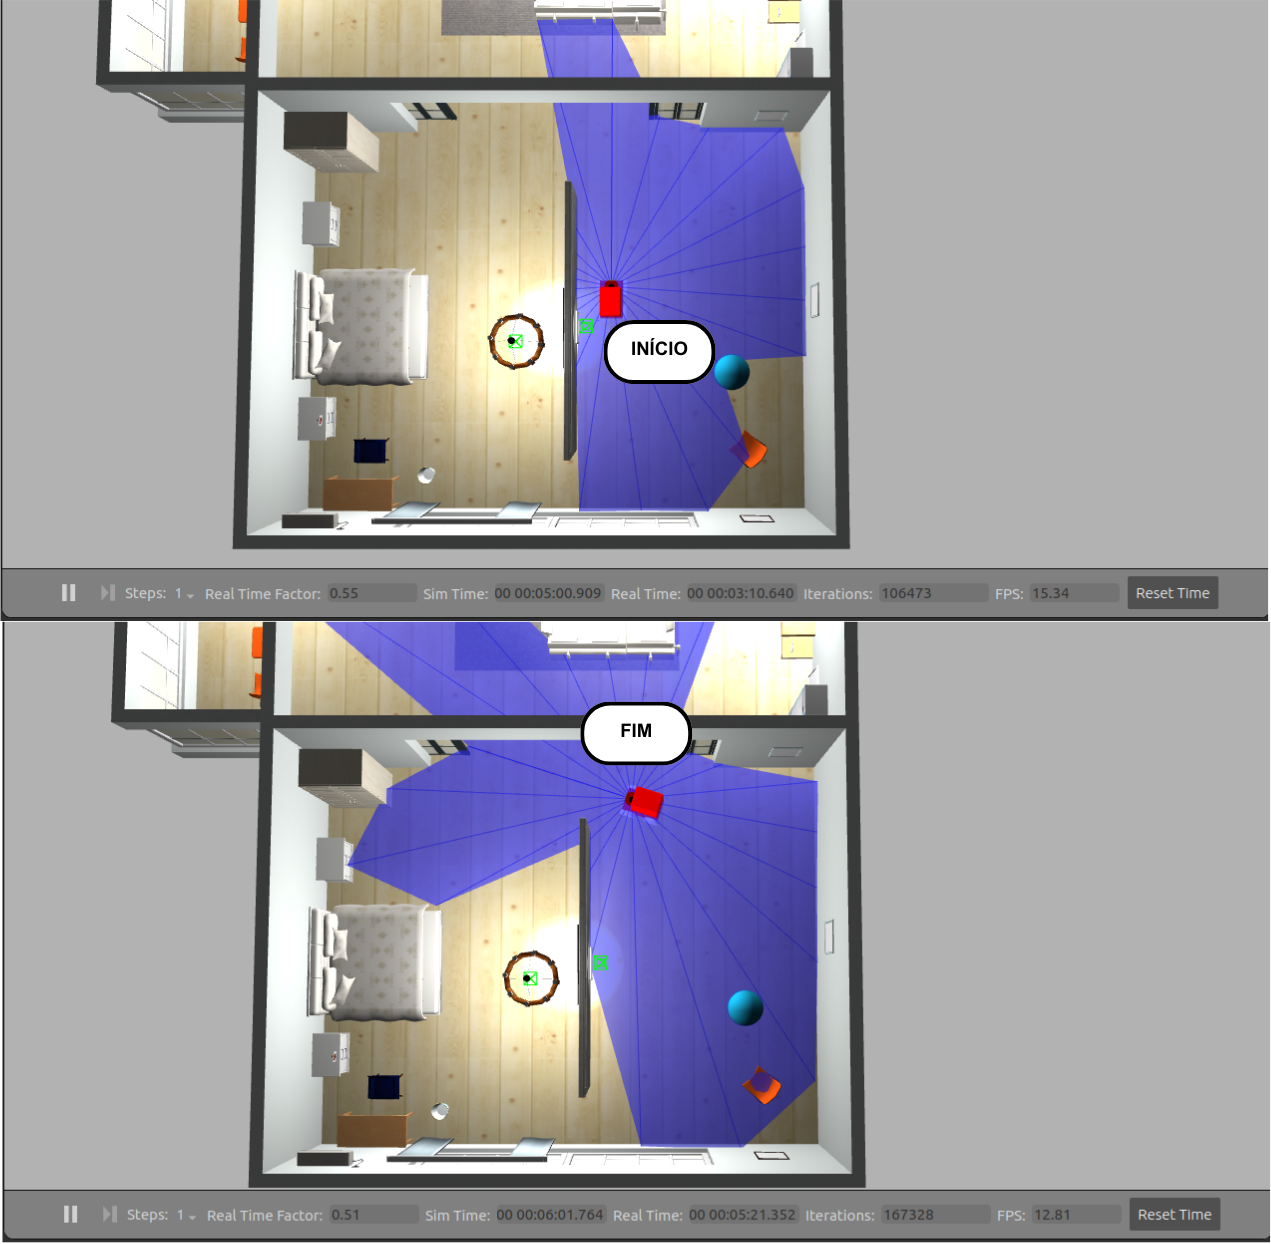
\includegraphics[scale=0.3]{ct02_1.png}
    \caption*{Fonte: Autora (2023).}
    \label{fig:teste1CT02}
\end{figure}

\begin{figure}[H]
    \centering
    \caption{Captura da primeira repetição CT03}
    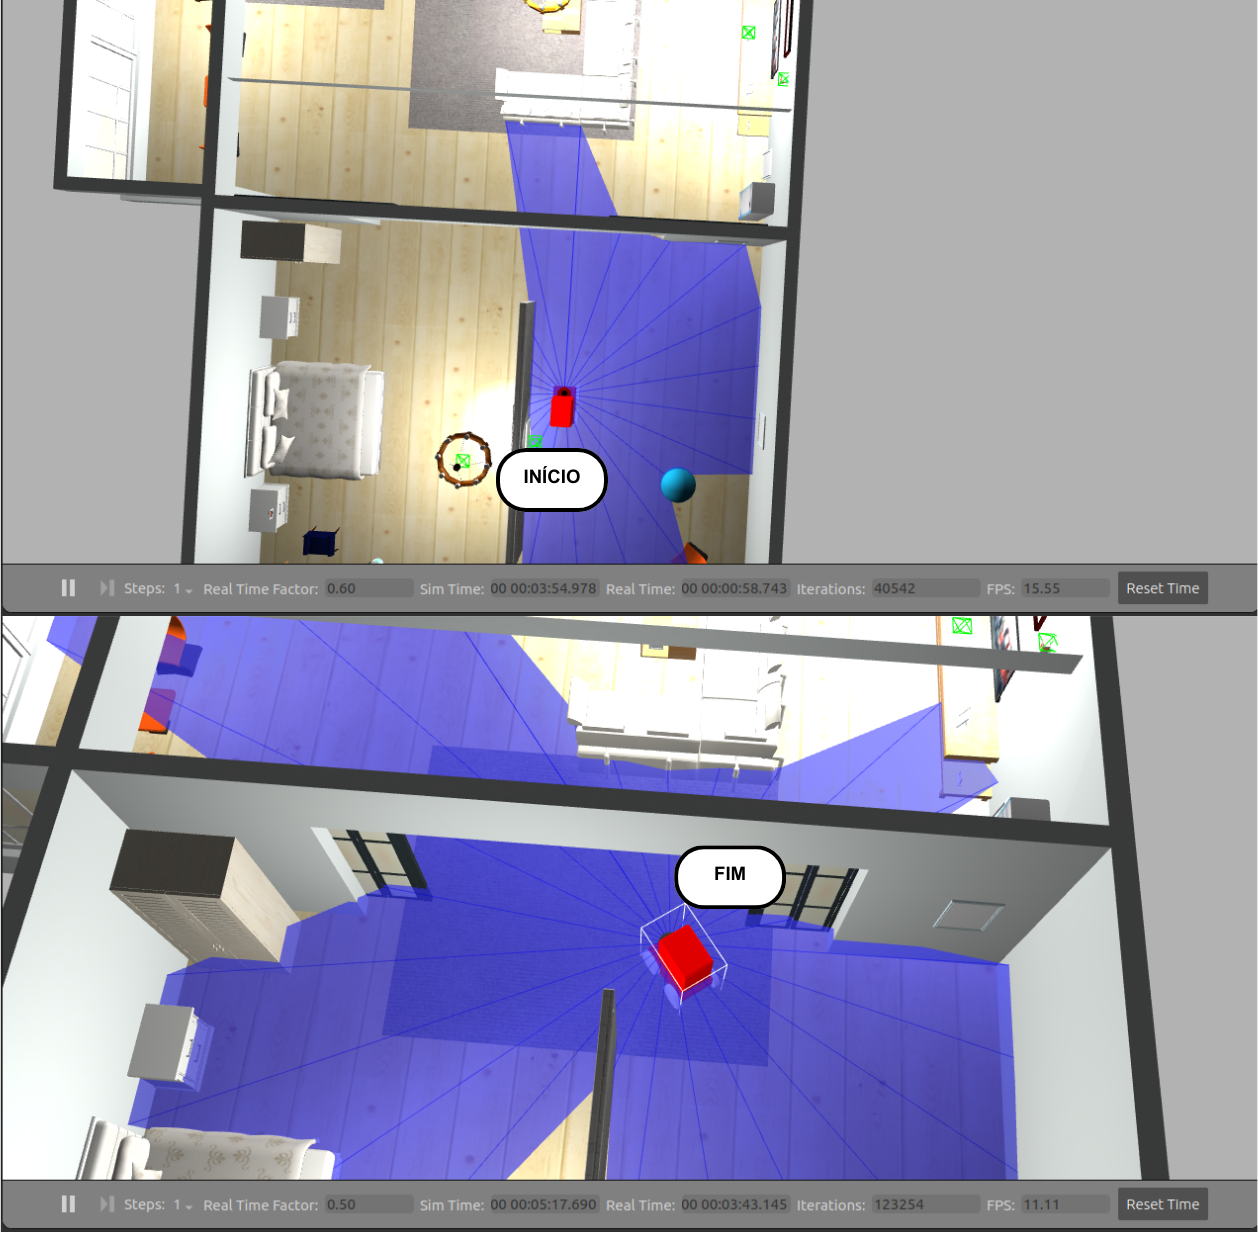
\includegraphics[scale=0.3]{ct03_1.png}
    \caption*{Fonte: Autora (2023).}
    \label{fig:teste1CT03}
\end{figure}

\begin{figure}[H]
    \centering
    \caption{Captura da primeira repetição CT04}
    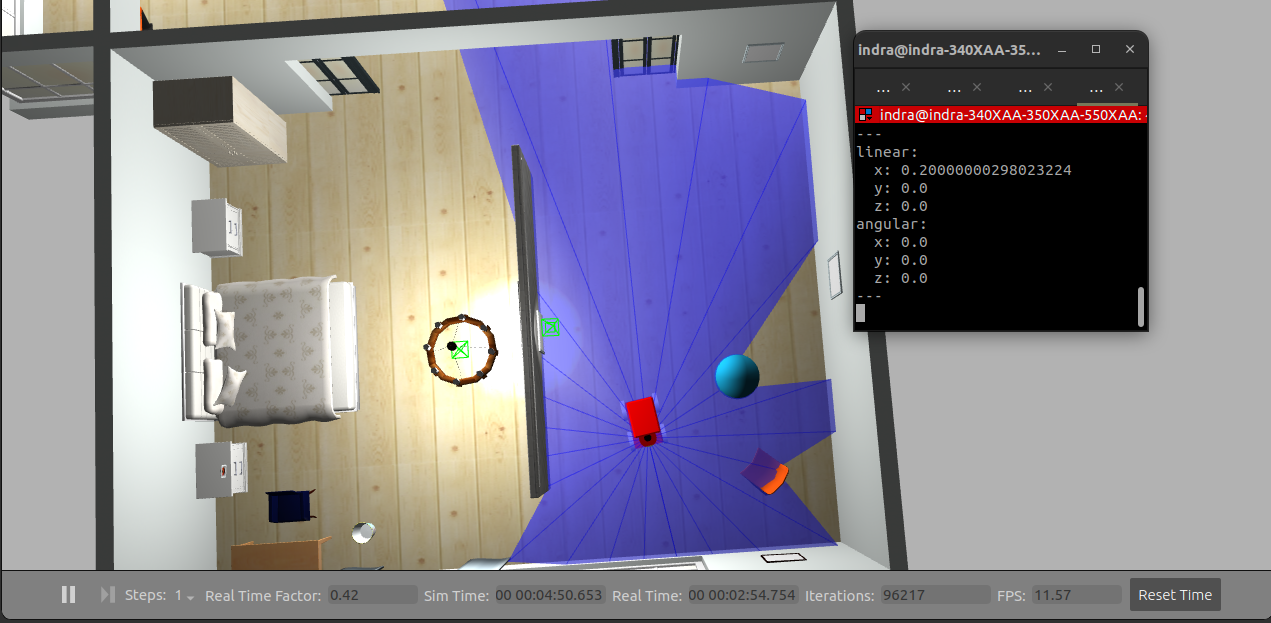
\includegraphics[scale=0.33]{ct04_1.png}
    \caption*{Fonte: Autora (2023).}
    \label{fig:teste1CT04}
\end{figure}

\begin{figure}[H]
    \centering
    \caption{Captura da primeira repetição CT05}
    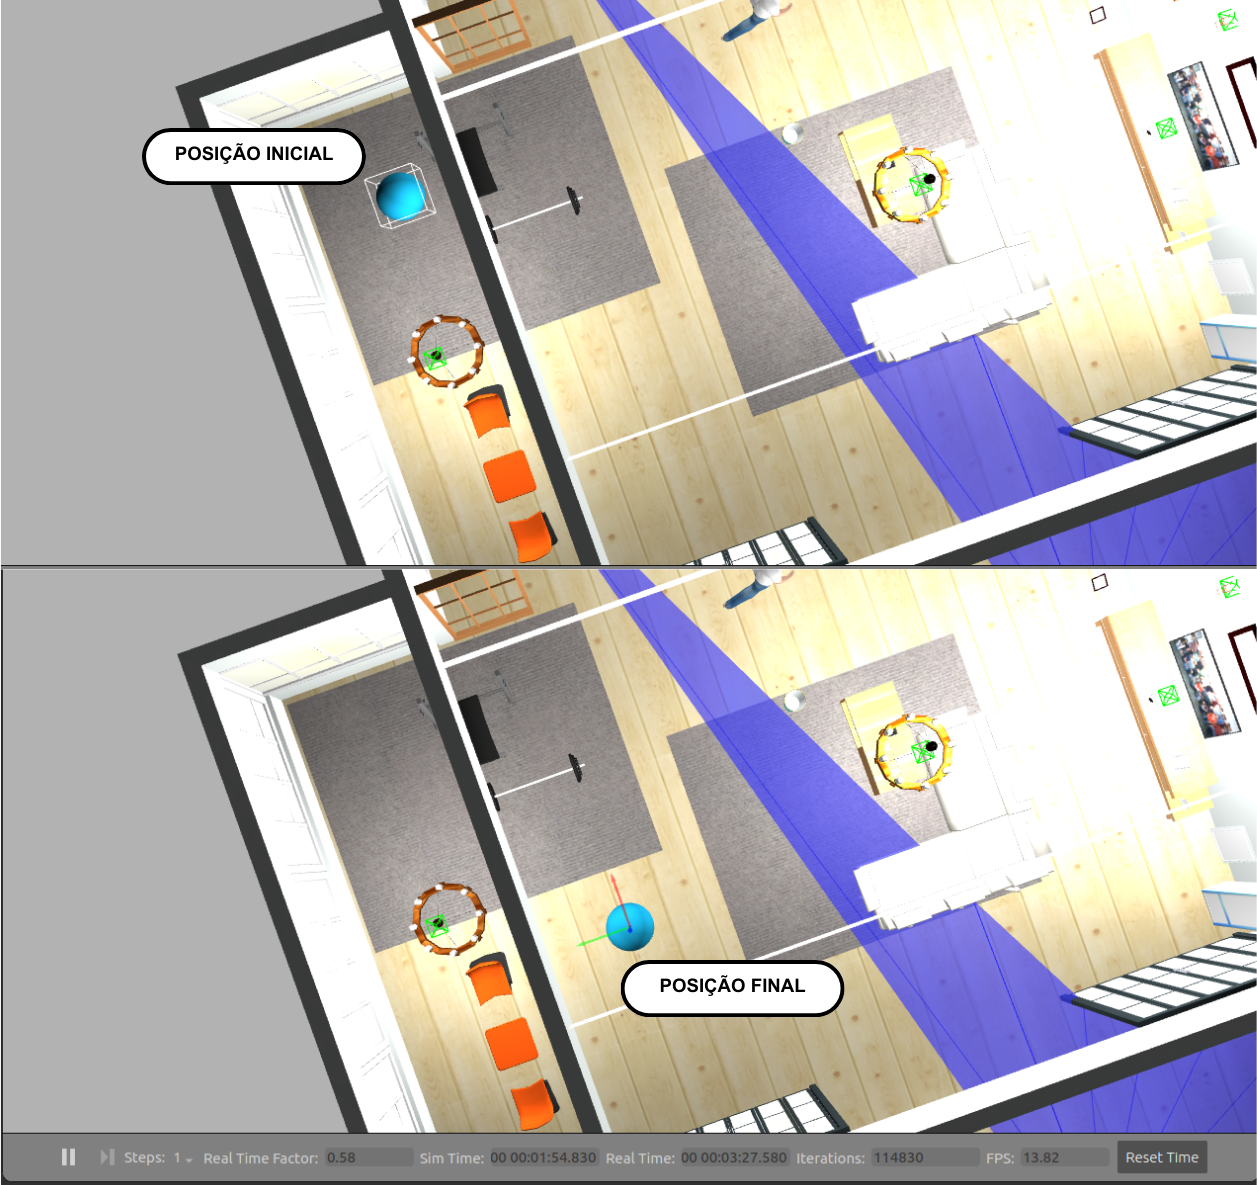
\includegraphics[scale=0.4]{ct05_1.png}
    \caption*{Fonte: Autora (2023).}
    \label{fig:teste1CT05}
\end{figure}

Dito isso, com as cinco repetições para os testes referentes aos casos de teste citados, foram obtidos apenas dois casos de teste com uma porcentagem de 80\% de sucesso. Dentre as 25 repetições de cinco casos de teste diferentes, os cenários CT01 e CT02  apresentaram uma taxa de sucesso menor que 100\%  (Figura~\ref{fig:sucessoTestes}).

\begin{figure}[h]
    \centering
    \caption{Resultados dos testes com repetições}
    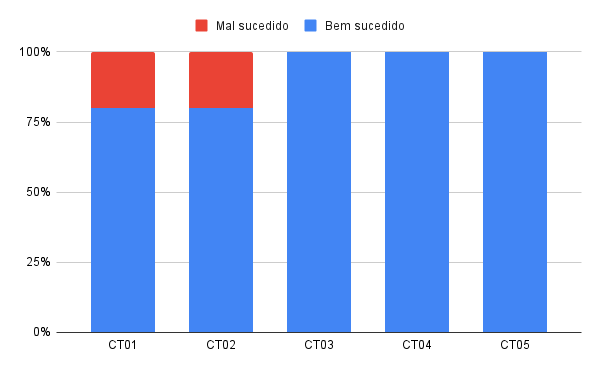
\includegraphics[scale=0.65]{sucessoTestes.png}
    \caption*{Fonte: Autora (2023).}
    \label{fig:sucessoTestes}
\end{figure}

Os casos de teste que obtiveram uma taxa de 80\% de sucesso correspondiam a capacidade do movimento do robô em todos os eixos e na sua locomoção pelo ambiente sem colidir com obstáculos. Os testes para o primeiro caso de teste (CT01) apresentaram uma falha de 20\%, ocasionada pelo mau posicionamento dos obstáculos (Figura~\ref{fig:erroCT01}).

\begin{figure}[p]
    \centering
    \caption{Captura da repetição do CT01 mal-sucedida }
    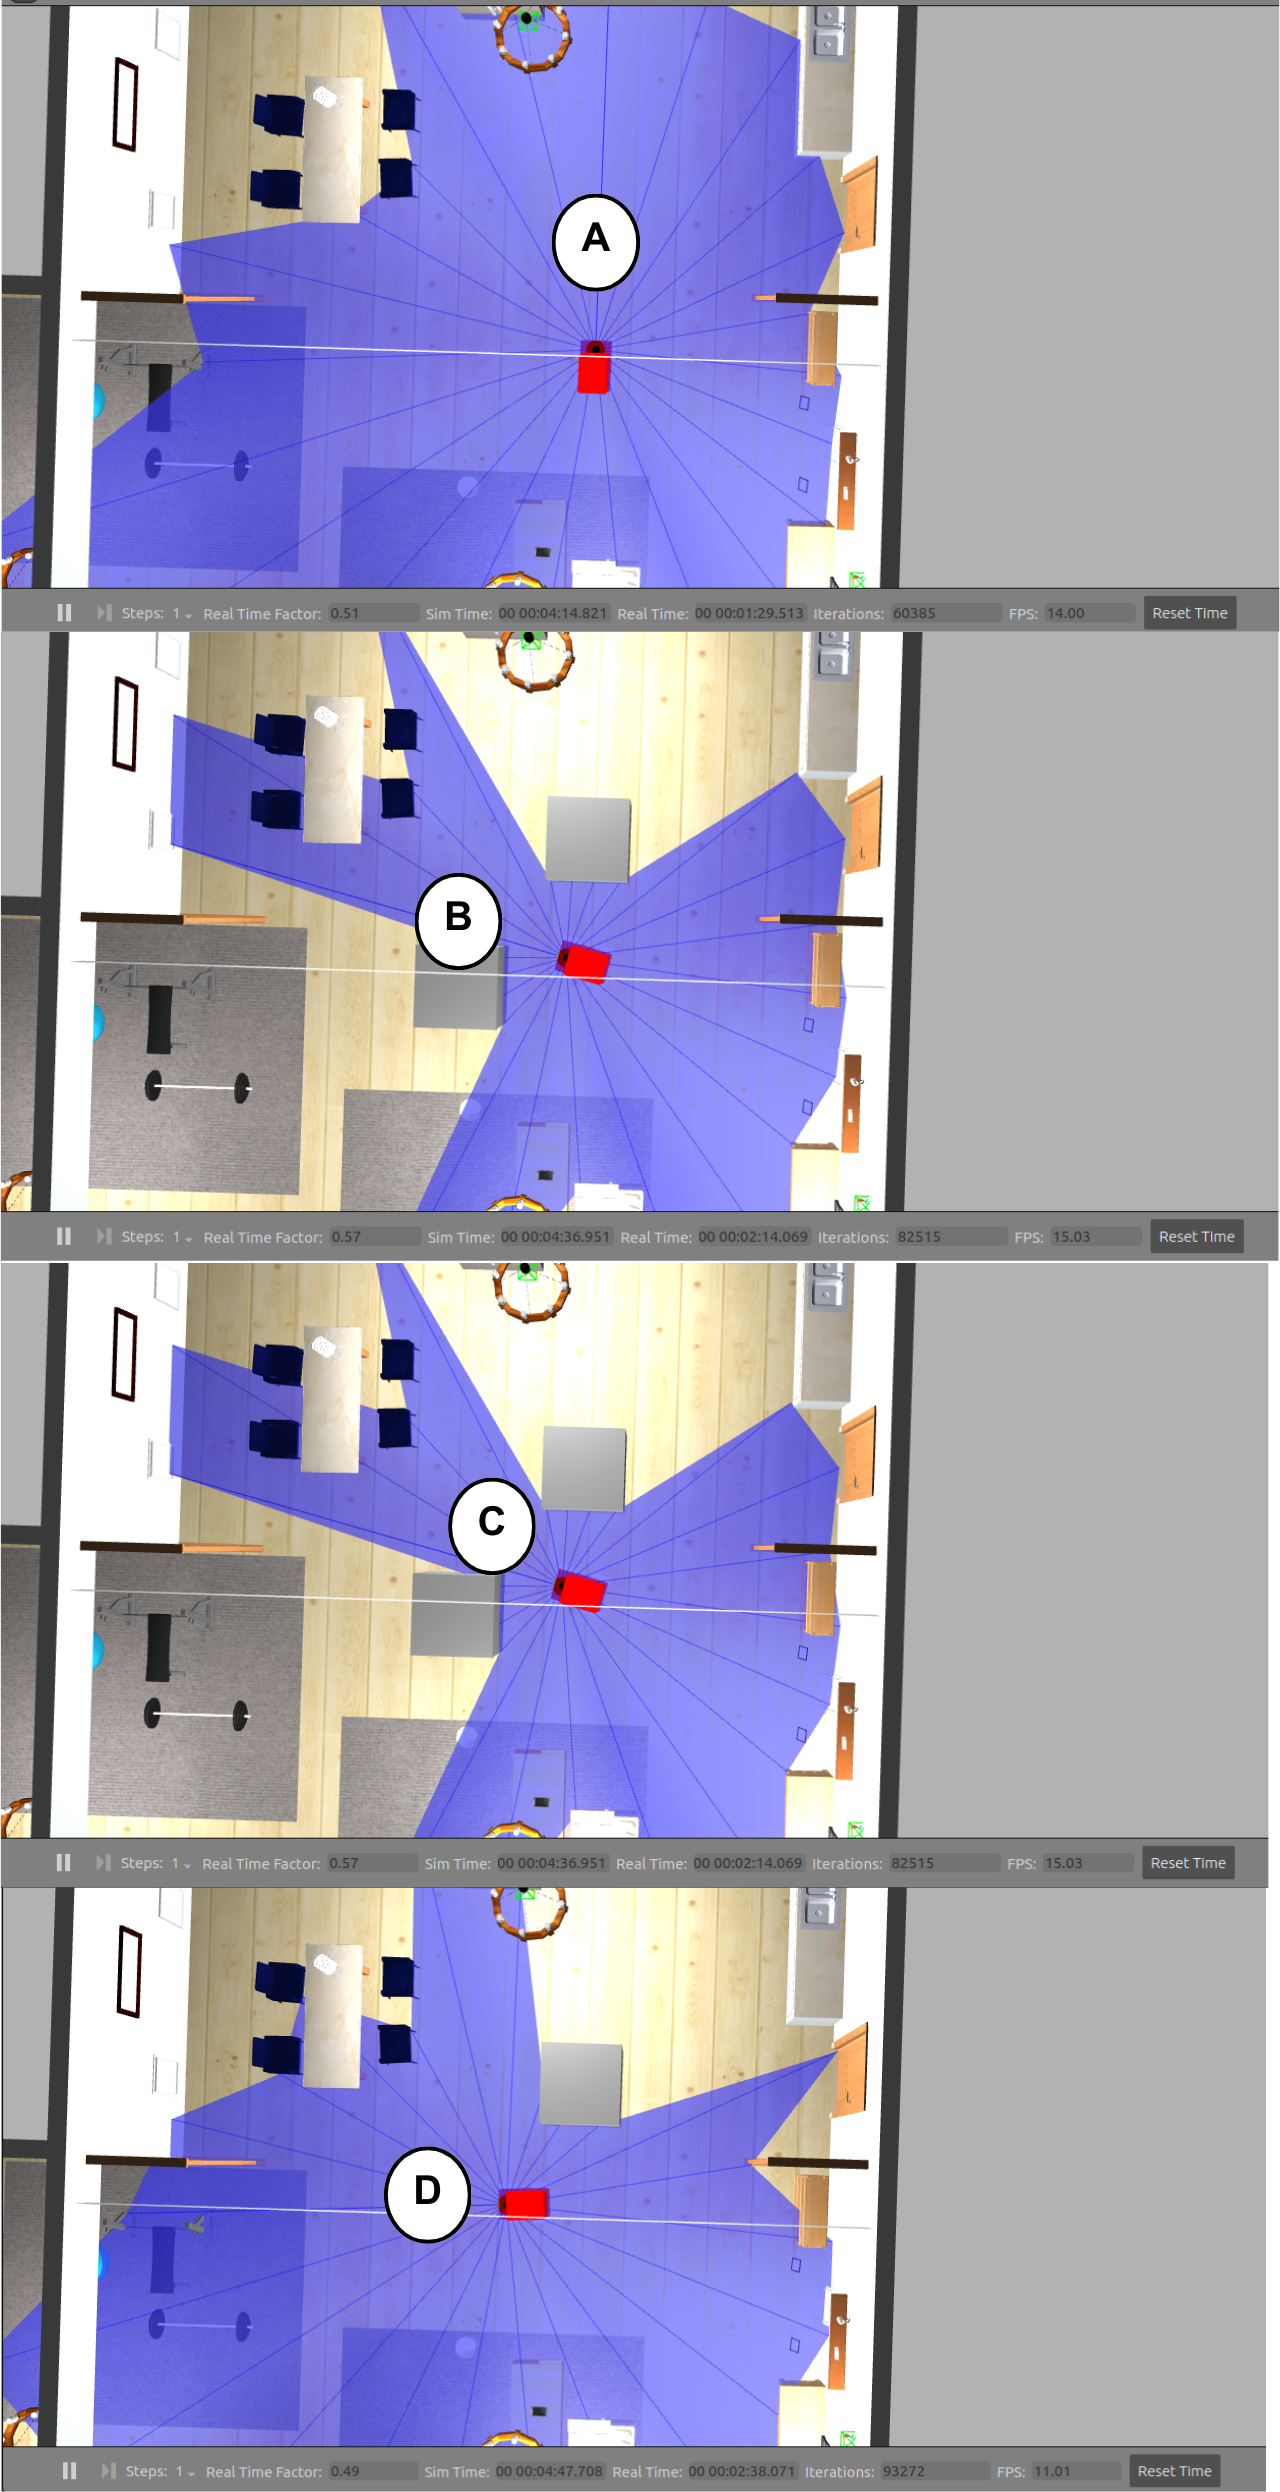
\includegraphics[scale=0.3]{ct01_4.png}
    \caption*{Fonte: Autora (2023).}
    \label{fig:erroCT01}
\end{figure}

O teste mal-sucedido para o segundo caso de teste (CT02), teve esse resultado devido ao local estreito na trajetória do robô (Figura~\ref{fig:erroCT02}). Para momentos no qual o robô se encontra sem opção, \citet{lidarRGBD} implementaram um estado de recuperação para que o robô possa retornar à sua navegação, podendo ser vantajoso em situações como a encontrada nesse teste com resultado negativo. Por ser uma porcentagem de falha mínima perante todos os sucessos, esses testes mal-sucedidos não impactam negativamente na navegação autônoma do robô. 

\begin{figure}[H]
    \centering
    \caption{Captura da repetição CT02 mal-sucedida}
    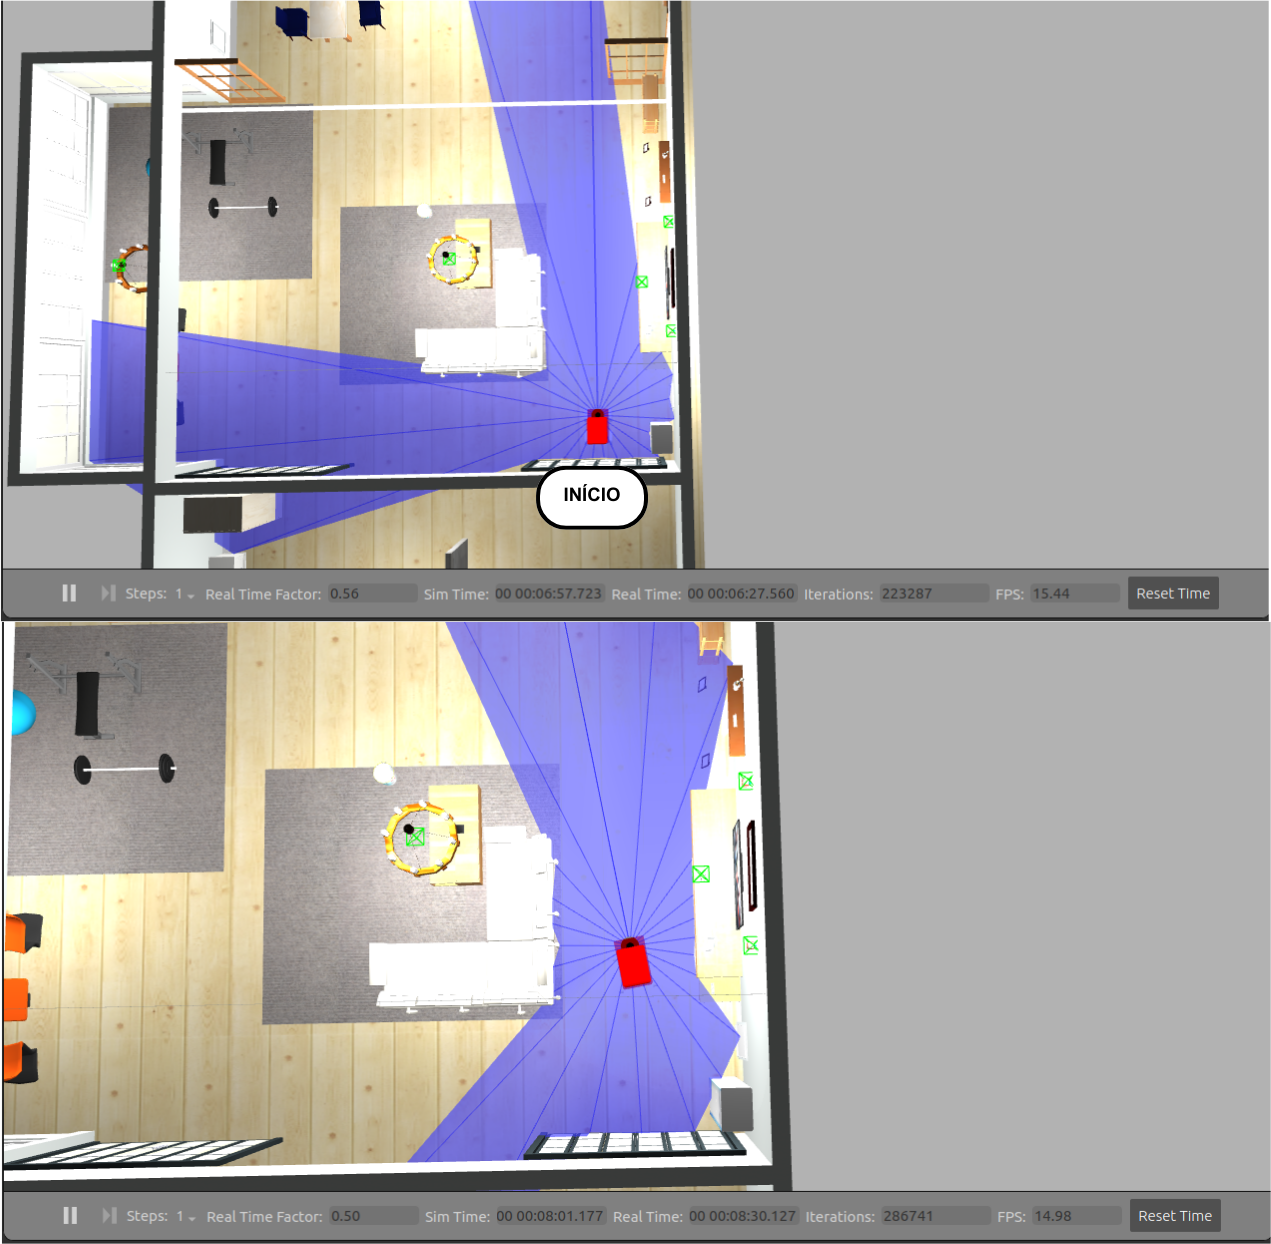
\includegraphics[scale=0.3]{ct02_4.png}
    \caption*{Fonte: Autora (2023).}
    \label{fig:erroCT02}
\end{figure}

Por fim, a simulação no programa Gazebo proporcionou a verificação da implementação das funcionalidades. Com isso, ao longo do desenvolvimento, foi possível analisar as integrações e realizar as mudanças necessárias para a melhoria dos componentes. Tal facilidade na validação do comportamento do robô pela simulação também é aproveitada por \citet{navegacaoSlam:2022, dpoom, lidarRGBD}. 


\chapter{Considerações Finais}
\label{cap-consideracoesFinais}

Este trabalho trouxe à tona o questionamento da possibilidade de desenvolver um robô de serviço doméstico com as tecnologias adequadas e relevantes, perante o atual momento caracterizado pelas teorias de  \textit{time-to-market} e do triângulo de ferro. Assim, foi identificado que, para esse desenvolvimento, é necessário modularizar o robô de serviço doméstico em funcionalidades independentes, se beneficiando de testes simulados para minimizar os recursos financeiros e o tempo despendido.


Dito isso, o presente trabalho conseguiu alcançar o seu objetivo geral definido com sucesso, sendo este elaborar um modelo de robô autônomo móvel simulado, capaz de realizar a funcionalidade fundamental de um robô de serviço doméstico: a navegação autônoma. O AtmosBot é formado por uma estrutura física com quatro rodas e um sensor LiDaR. Com as informações do sensor e da odometria das rodas, o robô tem a capacidade de mapear e se localizar no ambiente simulado desconhecido com abordagem SLAM ii) planejar e prosseguir por uma trajetória até um ponto de destino de forma autônoma sem colidir com obstáculos.

O desenvolvimento do modelo proposto foi possível a partir de uma revisão bibliográfica narrativa que fundamentou as teorias necessárias para a navegação autônoma e simulação robótica. Com as pesquisas bibliográficas constituídas por critérios pré-definidos, de inclusão e exclusão, foi possível analisar as tecnologias relevantes para a implementação de um robô autônomo móvel, alcançado o primeiro objetivo específico deste trabalho. Ademais, com os resultados dessas pesquisas bibliográficas específicas
foi encontrado que a abordagem SLAM é a mais implementada para a localização de um robô e o sensor LiDaR é o instrumento mais utilizado para a percepção de ambientes. Com isso,  foi implementado o SLAM e o sensor LiDaR para executar a navegação autônoma do robô, permitindo alcançar o segundo objetivo específico do presente trabalho. Por fim, o modelo integrado foi validado com sucesso por testes realizados conforme os casos de teste elaborados, expondo que todos os requisitos levantados foram atingidos. Além disso, foi realizada uma análise comparativa com os trabalhos correlatos encontrados, demonstrando que o modelo desenvolvido se comporta similarmente com propostas do mesmo âmbito, com uma redução de tempo e recursos despendidos. Portanto, destaca-se que todos os objetivos específicos definidos também foram alcançados com sucesso.

Confirmando a possibilidade de desenvolver moduladamente um robô de serviço doméstico com uma redução de recursos despendidos, conforme comprovado por este trabalho, é possível extrapolar tal ideia e considerar a probabilidade de tornar esses robôs mais acessíveis economicamente. Com isso, pode-se vislumbrar  que futuramente eles se tornem presentes até nas casas de pessoas de baixa renda com limitações motoras, auxiliando-as nas suas tarefas diárias e aumentando a sua qualidade de vida. 

Inicialmente foi idealizado o desenvolvimento de um modelo de robô autônomo móvel com capacidade de navegar autonomamente em direção a um objeto detectado no ambiente. As tecnologias mais relevantes no tema do trabalho seriam comparadas, por uma sequência de testes, a fim de identificar as ferramentas mais adequadas para cada sub-tarefa presente no sistema. Para condizer com o trabalho de conclusão de curso, o escopo foi reduzido para um robô autônomo móvel doméstico implementado com tecnologias selecionadas por uma análise de trabalhos correlatos. Além disso, o modelo implementa suas atuais funcionalidades de forma independente, podendo suportar incrementos de outras tarefas importantes para um robô de serviço doméstico. Diante disso, os requisitos do sistema foram identificados novamente para melhor suportar a solução proposta.

Dessa forma, este trabalho propõe um robô autônomo móvel doméstico independente capaz de ser integrado em um sistema maior para compor um robô de serviço doméstico. Assim, se vê como futuros trabalhos, a implementação de um módulo de localização e manipulação de objetos. Além disso, se torna viável a integração de uma interface para interação com humanos, possibilitando receber ordens de uma pessoa e executar atividades específicas em um ambiente, com o intuito de auxiliar nas suas tarefas diárias.

%
% O arquivo de formatação abntex2-alf.bst coloca todas as entradas no formato correto.
%

\bibliographystyle{abntex2-alf}
\bibliography{TEXTO-Bibliografia}

\appendix
\chapter{Documento de Especificação de Requisitos do Sistema}
\label{appendix-requisitos}
\section{Introdução}
Esta seção apresentará o propósito do documento de Especificação de Requisitos do Sistema, o escopo do sistema, as definições de termos, as abreviações e acrônimos, ademais da organização do documento.

\subsection{Propósito}
A Especificação de Requisitos do Sistema expõe as necessidades do robô autônomo móvel simulado que o trabalho propõe, assim como as exigências do ambiente simulado no qual o robô irá atuar. Com isso, será facilitada a implementação do modelo a ser proposto, além de permitir a realização de testes específicos e coerentes ao sistema. 

\subsection{Escopo}
O sistema AtmosBot inicial modelado é um robô autônomo móvel que atua em um ambiente interno dinâmico desconhecido. O agente deve conseguir realizar a tarefa elementar de um robô de serviço doméstico completamente autônomo, sendo ela: a navegação autônoma. Com isso, o robô simulado modelado deve ser capaz de se locomover pelo ambiente de forma autônoma e sem colidir com possíveis obstáculos.

\subsection{Definições}

RFS - Requisitos Funcionais do Sistema

RNFS - Requisitos Não Funcionais do Sistema

RNFA - Requisitos Não Funcionais do Ambiente

\subsection{Organização}
Este documento contém a descrição geral do projeto, incluindo a perspectiva do sistema, suas funções e as características do usuário. Ademais, possui os requisitos específicos funcionais e não funcionais subdivididos entre o sistema e o ambiente simulados.

\section{Descrição geral}
Esta seção descreve os fatores gerais que afetam o sistema e seus requisitos, contendo a perspectiva do sistema, as suas funções e as características do usuário.

\subsection{Perspectiva do sistema}
O sistema em questão funciona de forma independente para ser um robô autônomo móvel simulado. Entretanto, em um futuro trabalho, ele deve ser inserido como funcionalidade de um sistema maior que é um robô de serviço doméstico. 

Como boa prática, segundo os princípios da arquitetura de subsunção de \citet{brooks85}, cada funcionalidade de um robô de serviço doméstico deve ser independente e apenas realizar comunicações necessárias entre si. Então, o sistema a ser modelado deve funcionar de forma modular do projeto completo.

\subsection{Funções do sistema}
O dispositivo simulado deve conter duas funções essenciais ao seu funcionamento, sendo elas:
\begin{enumerate}
    \item Navegação autônoma pelo ambiente sem colidir com obstáculos;
    \item Exploração do ambiente.
\end{enumerate}
Todas as sub-tarefas fundamentais das funções supracitadas devem ser cumpridas integralmente para o funcionamento correto do sistema.

\subsection{Características do usuário}
O sistema descrito é autônomo e não necessita da interação ou interferência de usuários humanos. Ele atua unicamente no ambiente inserido conforme as características do mesmo.

\section{Requisitos específicos}
Esta seção destaca com detalhe todos os requisitos funcionais e não funcionais do robô móvel autônomo simulado e do ambiente que será criado por simulação a fim de testar o sistema proposto. Os requisitos funcionais determinam as ações fundamentais que o sistema e o ambiente devem ter para que o dispositivo a ser modelado consiga aceitar e processar as suas entradas, além de gerar saídas para seus atuadores agirem no meio. 

Os requisitos não funcionais englobam questões de desempenho, segurança, confiabilidade, entre outros aspectos que são características necessárias para um ótimo funcionamento geral, não conceituando ações do sistema.

Todos os requisitos são rotulados pela prioridade e urgência de aplicação, podendo ser definidos como:
\begin{itemize}
    \item Essencial: o requisito não pode faltar no sistema ou ambiente;
    \item Importante: o requisito é necessário para um bom funcionamento, porém não o limita;
    \item Desejável: o requisito é necessário para um ótimo funcionamento, mas pode ser implementado em uma futura versão sem impactar o desempenho do sistema.
\end{itemize}
Além disso, os requisitos são expostos segundo a Tabela \ref{tab:modeloRequisitos}.

\begin{table}[H]
\centering
\caption{Modelo dos requisitos}
\label{tab:modeloRequisitos}
\resizebox{\textwidth}{!}{%
\begin{tabular}{l|p{15cm}|l}
\textbf{Identificação do requisito} & \textbf{Título do requisito}                    & \textbf{Prioridade}                   \\ \hline
\textbf{Entrada}                    & \multicolumn{2}{p{17cm}}{Especificação da entrada necessária para a funcionalidade}           \\ \hline
\textbf{Detalhamento}               & \multicolumn{2}{p{17cm}}{Detalhamento da funcionalidade}                                      \\ \hline
\textbf{Saída}                      & \multicolumn{2}{p{17cm}}{Especificação da saída necessária após a execução da funcionalidade} \\ \hline
\end{tabular}%
}
\caption*{Fonte: Autora (2023).}
\end{table}

\subsection{Requisitos Funcionais do Sistema}

\begin{table}[H]
\centering
\caption{RFS01}
\resizebox{\textwidth}{!}{%
\begin{tabular}{l|p{15cm}|l}
\textbf{RFS01} & \textbf{Movimentação do robô}                    & \textbf{Importante}                   \\ \hline
\textbf{Entrada}                    & \multicolumn{2}{p{17cm}}{Direção definida pelo eixo que o robô precisa se locomover.}           \\ \hline
\textbf{Detalhamento}               & \multicolumn{2}{p{17cm}}{O robô deve se mover para todas as direções no ambiente.}                                      \\ \hline
\textbf{Saída}                      & \multicolumn{2}{p{17cm}}{Movimentação do instrumento de locomoção (rodas ou pernas) do robô conforme a direção explicitada.} \\ \hline
\end{tabular}% 
}
\caption*{Fonte: Autora (2023).}
\end{table}

\begin{table}[H]
\centering
\caption{RFS02}
\resizebox{\textwidth}{!}{%
\begin{tabular}{l|p{15cm}|l}
\textbf{RFS02} & \textbf{Evitação de obstáculos}                    & \textbf{Essencial}                   \\ \hline
\textbf{Entrada}                    & \multicolumn{2}{p{17cm}}{Dados do ambiente ao redor do robô coletados a partir de sensores em seu corpo.}           \\ \hline
\textbf{Detalhamento}               & \multicolumn{2}{p{17cm}}{O robô deve processar os dados dos sensores de modo a saber se há um obstáculo (objeto, pessoa, animal, parede ou móvel) perto o suficiente que ele possa colidir. Com essa informação, caso haja um obstáculo próximo a sua frente, o robô deve se esquivar dele e continuar sua trajetória planejada. Caso não haja obstáculos a sua frente, o robô deve continuar a sua trajetória planejada.}                                      \\ \hline
\textbf{Saída}                      & \multicolumn{2}{p{17cm}}{Comandos para os motores atuarem nas rodas alterando a direção conforme o obstáculo detectado.} \\ \hline
\end{tabular}% 
}
\caption*{Fonte: Autora (2023).}
\end{table}


\begin{table}[H]
\centering
\caption{RNFS01}
\resizebox{\textwidth}{!}{%
\begin{tabular}{l|p{15cm}|l}
\textbf{RNFS01} & \textbf{Locomoção em diferentes superfícies}                    & \textbf{Importante}                   \\ \hline
\textbf{Entrada}                    & \multicolumn{2}{p{17cm}}{Não possui.}           \\ \hline
\textbf{Detalhamento}               & \multicolumn{2}{p{17cm}}{O robô deve ser capaz de se locomover de forma satisfatória, tanto em pisos lisos,  quanto em pisos revestidos (com carpetes ou tapetes).}                                      \\ \hline
\textbf{Saída}                      & \multicolumn{2}{p{17cm}}{Não possui.} \\ \hline
\end{tabular}% 
}
\caption*{Fonte: Autora (2023).}
\end{table}

\begin{table}[H]
\centering
\caption{RNFS02}
\resizebox{\textwidth}{!}{%
\begin{tabular}{l|p{15cm}|l}
\textbf{RNFS02}& \textbf{Locomoção com segurança aos seres transeuntes}                    & \textbf{Desejável}                   \\ \hline
\textbf{Entrada}                    & \multicolumn{2}{p{17cm}}{Não possui.}           \\ \hline
\textbf{Detalhamento}               & \multicolumn{2}{p{17cm}}{A velocidade de locomoção do robô deve ser moderada, respeitando o ambiente interno e sua dinamicidade, a fim de não prejudicar as pessoas e/ou animais que transitam o espaço em conjunto com o próprio robô. Sendo assim, ela não deve ultrapassar de 0,2 m/s. }                                      \\ \hline
\textbf{Saída}                      & \multicolumn{2}{p{17cm}}{Não possui.} \\ \hline
\end{tabular}% 
}
\caption*{Fonte: Autora (2023).}
\end{table}


\subsection{Requisitos Não Funcionais do Ambiente Simulado}


\begin{table}[H]
\centering
\caption{RNFA01}
\resizebox{\textwidth}{!}{%
\begin{tabular}{l|p{15cm}|l}
\textbf{RNFA01} & \textbf{Dinamicidade}                    & \textbf{Essencial}                   \\ \hline
\textbf{Entrada}                    & \multicolumn{2}{p{17cm}}{Não possui.}           \\ \hline
\textbf{Detalhamento}               & \multicolumn{2}{p{17cm}}{O ambiente deve conter mudanças frequentes na posição de objetos e móveis.}                                      \\ \hline
\textbf{Saída}                      & \multicolumn{2}{p{17cm}}{Não possui.} \\ \hline
\end{tabular}% 
}
\caption*{Fonte: Autora (2023).}
\end{table}


\begin{table}[H]
\centering
\caption{RNFA02}
\resizebox{\textwidth}{!}{%
\begin{tabular}{l|p{15cm}|l}
\textbf{RNFA02} & \textbf{Semelhança a domicílios reais}                    & \textbf{Essencial}                   \\ \hline
\textbf{Entrada}                    & \multicolumn{2}{p{17cm}}{Não possui.}           \\ \hline
\textbf{Detalhamento}               & \multicolumn{2}{p{17cm}}{O ambiente deve trazer aspectos de um domicílio comum, com móveis, paredes, portas, objetos, tapetes, entre outros itens que o tornam mais verossímil à realidade.}                                      \\ \hline
\textbf{Saída}                      & \multicolumn{2}{p{17cm}}{Não possui.} \\ \hline
\end{tabular}% 
}
\caption*{Fonte: Autora (2023).}
\end{table}

\begin{table}[H]
\centering
\caption{RNFA03}
\resizebox{\textwidth}{!}{%
\begin{tabular}{l|p{15cm}|l}
\textbf{RNFA03} & \textbf{Tamanho de domicílio padrão}                    & \textbf{Desejável}                   \\ \hline
\textbf{Entrada}                    & \multicolumn{2}{p{17cm}}{Não possui.}           \\ \hline
\textbf{Detalhamento}               & \multicolumn{2}{p{17cm}}{O ambiente deve conter, no mínimo, três cômodos internos que se conectam de alguma forma (por portas ou corredores).}                                      \\ \hline
\textbf{Saída}                      & \multicolumn{2}{p{17cm}}{Não possui.} \\ \hline
\end{tabular}% 
}
\caption*{Fonte: Autora (2023).}
\end{table}

\begin{table}[H]
\centering
\caption{RNFA04}
\resizebox{\textwidth}{!}{%
\begin{tabular}{l|p{15cm}|l}
\textbf{RNFA04}& \textbf{Minimização de Impedimentos}                    & \textbf{Essencial}                   \\ \hline
\textbf{Entrada}                    & \multicolumn{2}{p{17cm}}{Não possui.}           \\ \hline
\textbf{Detalhamento}               & \multicolumn{2}{p{17cm}}{O ambiente não deve conter portas fechadas ou pouco abertas. Além disso o ambiente de acesso do robô não deve conter escadas ou degraus altos (devem conter no máximo 1 centímetro de altura).}                                      \\ \hline
\textbf{Saída}                      & \multicolumn{2}{p{17cm}}{Não possui.} \\ \hline
\end{tabular}% 
}
\caption*{Fonte: Autora (2023).}
\end{table}


\chapter{Detalhamento dos Casos de Teste}
\label{appendix-casosTeste}
\section{Introdução}
Este apêndice tem o intuito de explicar e expor os casos de teste definidos para realizar a validação final do modelo proposto para um robô autônomo móvel perante os requisitos previamente definidos para o sistema completo (robô e ambiente simulados).

\section{Casos de teste}
Os casos de teste são procedimentos para realizar testes nos quais são dispostos as ações necessárias para realizar cada teste e o resultado ideal perante estas ações.
Para melhor organização e padronização, os casos de teste aqui definidos seguem o modelo disposto na Tabela  \ref{tab:modeloCasos}.

\begin{table}[H]
\centering
\caption{Modelo dos casos de teste}
\label{tab:modeloCasos}
\resizebox{\textwidth}{!}{%
\begin{tabular}{p{3cm}|p{5cm}|p{5cm}}
\multicolumn{1}{p{3cm}|}{\textbf{Requisito referente}} &
  \multicolumn{1}{p{5cm}|}{\textbf{Ação/Entrada}} &
  \multicolumn{1}{p{5cm}}{\textbf{Resultado esperado}} \\ \hline
Título do requisito ao que o caso de teste se refere. &
  Detalhamento da ação, ou entrada, necessária para validar o requisito. &
  Detalhamento do Resultado esperado da simulação perante a ação, ou entrada, definida. \\ \hline
\end{tabular}%
}
\caption*{Fonte: Autora (2023).}
\end{table}

A seguir são dispostos os casos de teste elaborados conforme os requisitos (funcionais e não funcionais) definidos previamente para a simulação do ambiente e do robô, expostos no \appendixautorefname~\ref{appendix-requisitos}.

\begin{table}[p]
\centering
\caption{Caso de teste CT01 referente a RFS01 }
\label{tab:caso01}
\resizebox{\textwidth}{!}{%
\begin{tabular}{p{3cm}|p{5cm}|p{5cm}}
\multicolumn{1}{p{3cm}|}{\textbf{Requisito referente}} &
  \multicolumn{1}{p{5cm}|}{\textbf{Ação/Entrada}} &
  \multicolumn{1}{p{5cm}}{\textbf{Resultado esperado}} \\ \hline
Movimentação do robô &
  Em primeiro lugar, a simulação deve ser executada e o estado de vagar pelo ambiente deve ser inciado. Com tudo executando devidamente, devem ser adicionados obstáculos há 0,5 metros da dianteira e lateral esquerda do robô. Após 5 segundos, devem ser adicionados obstáculos há 0,5 metros da dianteira e lateral direita do robô. &
  Ao adicionar os primeiros obstáculos, o robô deverá se rotacionar no sentido direito. Após adicionar os últimos obstáculos, o robô deverá se rotacionar no sentido esquerdo.
  \\ \hline
\end{tabular}%
}
\caption*{Fonte: Autora (2023).}
\end{table}


\begin{table}[p]
\centering
\caption{Caso de teste CT02 referente a RFS02 }
\label{tab:caso02}
\resizebox{\textwidth}{!}{%
\begin{tabular}{p{3cm}|p{5cm}|p{5cm}}
\multicolumn{1}{p{3cm}|}{\textbf{Requisito referente}} &
  \multicolumn{1}{p{5cm}|}{\textbf{Ação/Entrada}} &
  \multicolumn{1}{p{5cm}}{\textbf{Resultado esperado}} \\ \hline
Evitação de obstáculos &
  Em primeiro lugar, a simulação deve ser executada e o estado de exploração do ambiente deve ser inciado. A exploração deve ocorrer por 120 segundos. &
  Com o ambiente propriamente elaborado, o robô deverá se locomover por ele e se esquivar de possíveis móveis que estão presentes no meio.
  \\ \hline
\end{tabular}%
}
\caption*{Fonte: Autora (2023).}
\end{table}

\begin{table}[p]
\centering
\caption{Caso de teste CT03 referente a RNFS01 }
\label{tab:caso04}
\resizebox{\textwidth}{!}{%
\begin{tabular}{p{3cm}|p{5cm}|p{5cm}}
\multicolumn{1}{p{3cm}|}{\textbf{Requisito referente}} &
  \multicolumn{1}{p{5cm}|}{\textbf{Ação/Entrada}} &
  \multicolumn{1}{p{5cm}}{\textbf{Resultado esperado}} \\ \hline
Locomoção em diferentes superfícies  &
  Em primeiro lugar, a simulação deve ser executada e o estado de vagar pelo ambiente deve ser inciado em um meio constituído parcialmente por piso liso e por tapete. &
  O robô deverá se movimentar igualmente em ambos as superfícies, sem que o robô apresente o comportamente de instabilidade nas rodas ou emperramento.
  \\ \hline
\end{tabular}%
}
\caption*{Fonte: Autora (2023).}
\end{table}

\begin{table}[p]
\centering
\caption{Caso de teste CT04 referente a RNFS02 }
\label{tab:caso05}
\resizebox{\textwidth}{!}{%
\begin{tabular}{p{3cm}|p{5cm}|p{5cm}}
\multicolumn{1}{p{3cm}|}{\textbf{Requisito referente}} &
  \multicolumn{1}{p{5cm}|}{\textbf{Ação/Entrada}} &
  \multicolumn{1}{p{5cm}}{\textbf{Resultado esperado}} \\ \hline
Locomoção com segurança aos seres transeuntes  &
  Em primeiro lugar, a simulação deve ser executada e o estado de exploração do ambiente deve ser inciado em um meio constituído por no mínimo um ser humano se locomovendo. &
  O robô deverá se locomover pelo ambiente em uma velocidade até 0,2 m/s.
  \\ \hline
\end{tabular}%
}
\caption*{Fonte: Autora (2023).}
\end{table}


\begin{table}[p]
\centering
\caption{Caso de teste CT05 referente a RNFA01 }
\label{tab:caso07}
\resizebox{\textwidth}{!}{%
\begin{tabular}{p{3cm}|p{5cm}|p{5cm}}
\multicolumn{1}{p{3cm}|}{\textbf{Requisito referente}} &
  \multicolumn{1}{p{5cm}|}{\textbf{Ação/Entrada}} &
  \multicolumn{1}{p{5cm}}{\textbf{Resultado esperado}} \\ \hline
Dinamicidade  &
  Em primeiro lugar, a simulação deve ser executada e a posição dos objetos e móveis devem ser alteradas com constância.   &
  Os objetos e móveis deverão ter sua posição alterada sem que a simulação pare ou corrompa. 
  \\ \hline
\end{tabular}%
}
\caption*{Fonte: Autora (2023).}
\end{table}


\begin{table}[p]
\centering
\caption{Caso de teste CT06 referente a RNFA03 }
\label{tab:caso09}
\resizebox{\textwidth}{!}{%
\begin{tabular}{p{3cm}|p{5cm}|p{5cm}}
\multicolumn{1}{p{3cm}|}{\textbf{Requisito referente}} &
  \multicolumn{1}{p{5cm}|}{\textbf{Ação/Entrada}} &
  \multicolumn{1}{p{5cm}}{\textbf{Resultado esperado}} \\ \hline
Semelhança a domicílios reais  &
  A simulação deve ser executada.   &
  A simulação deverá apresentar uma planta residencial básica com elementos de sala, dormitório e cozinha.
  \\ \hline
\end{tabular}%
}
\caption*{Fonte: Autora (2023).}
\end{table}

\begin{table}[p]
\centering
\caption{Caso de teste CT07 referente a RNFA04 }
\label{tab:caso10}
\resizebox{\textwidth}{!}{%
\begin{tabular}{p{3cm}|p{5cm}|p{5cm}}
\multicolumn{1}{p{3cm}|}{\textbf{Requisito referente}} &
  \multicolumn{1}{p{5cm}|}{\textbf{Ação/Entrada}} &
  \multicolumn{1}{p{5cm}}{\textbf{Resultado esperado}} \\ \hline
Tamanho de domicílio padrão  &
  A simulação deve ser executada.   &
  O ambiente simulado deverá apresentar no mínimo um espaço de cozinha, sala e dormitório. Entre os espaços, não devem se apresentar portas de acesso fechadas.
  \\ \hline
\end{tabular}
%
}
\caption*{Fonte: Autora (2023).}
\end{table}

\begin{table}[p]
\centering
\caption{Caso de teste CT08 referente a RNFA05 }
\label{tab:caso11}
\resizebox{\textwidth}{!}{%
\begin{tabular}{p{3cm}|p{5cm}|p{5cm}}
\multicolumn{1}{p{3cm}|}{\textbf{Requisito referente}} &
  \multicolumn{1}{p{5cm}|}{\textbf{Ação/Entrada}} &
  \multicolumn{1}{p{5cm}}{\textbf{Resultado esperado}} \\ \hline
Minimização de Impedimentos  &
  A simulação deve ser executada.   &
  O ambiente simulado não deverá apresentar portas de acesso, entre os espaços, que se apresentam fechadas.
  \\ \hline
\end{tabular}
%
}
\caption*{Fonte: Autora (2023).}
\end{table}

\chapter{Resultados dos Testes}
\label{appendix-resultadosTestes}
Este apêndice tem o intuito de expor os resultados obtidos por testes de validação do modelo proposto. Esses testes foram realizados conforme detalhado nos casos de teste, apresentados no \appendixautorefname~\ref{appendix-casosTeste}.

\section{Caso de Teste CT01 Referente a RFS01}
O caso de teste CT01 visou validar se o robô é capaz de se mover para todos os sentidos e direções pelo ambiente que está inserido. O caso de teste foi repetido cinco vezes com o robô em lugares distintos no ambiente. Entre os cinco testes, apenas um foi mal sucedido, visto que o robô rotacionou para o lado errado ao adicionar os obstáculos. Todos os resultados podem ser visualizados na Tabela~\ref{tab:acertosct01}. Além disso, a seguir podem ser encontradas as capturas para cada repetição (Figura~\ref{fig:ct01_1}, Figura~\ref{fig:ct01_2}, Figura~\ref{fig:ct01_3}, Figura~\ref{fig:ct01_4}, Figura~\ref{fig:ct01_5}).

\begin{table}[H]
\centering
\caption{Resultados das repetições CT01}
\label{tab:acertosct01}
\resizebox{\textwidth}{!}{%
\begin{tabular}{l|c}
                              & \multicolumn{1}{l}{\textbf{Resultados CT01}} \\ \hline
\textbf{Teste 1}              & Bem-sucedido                                 \\
\textbf{Teste 2}              & Bem-sucedido                                 \\
\textbf{Teste 3}              & Bem-sucedido                                 \\
\textbf{Teste 4}              & Mal-sucedido                                 \\
\textbf{Teste 5}              & Bem-sucedido                                 \\
\textbf{Total de acertos (\%)} & \textbf{80}                                  \\ \hline
\end{tabular}%
}
\caption*{Fonte: Autora (2023).}
\end{table}

\begin{figure}[H]
    \centering
    \caption{Captura da primeira repetição CT01}
    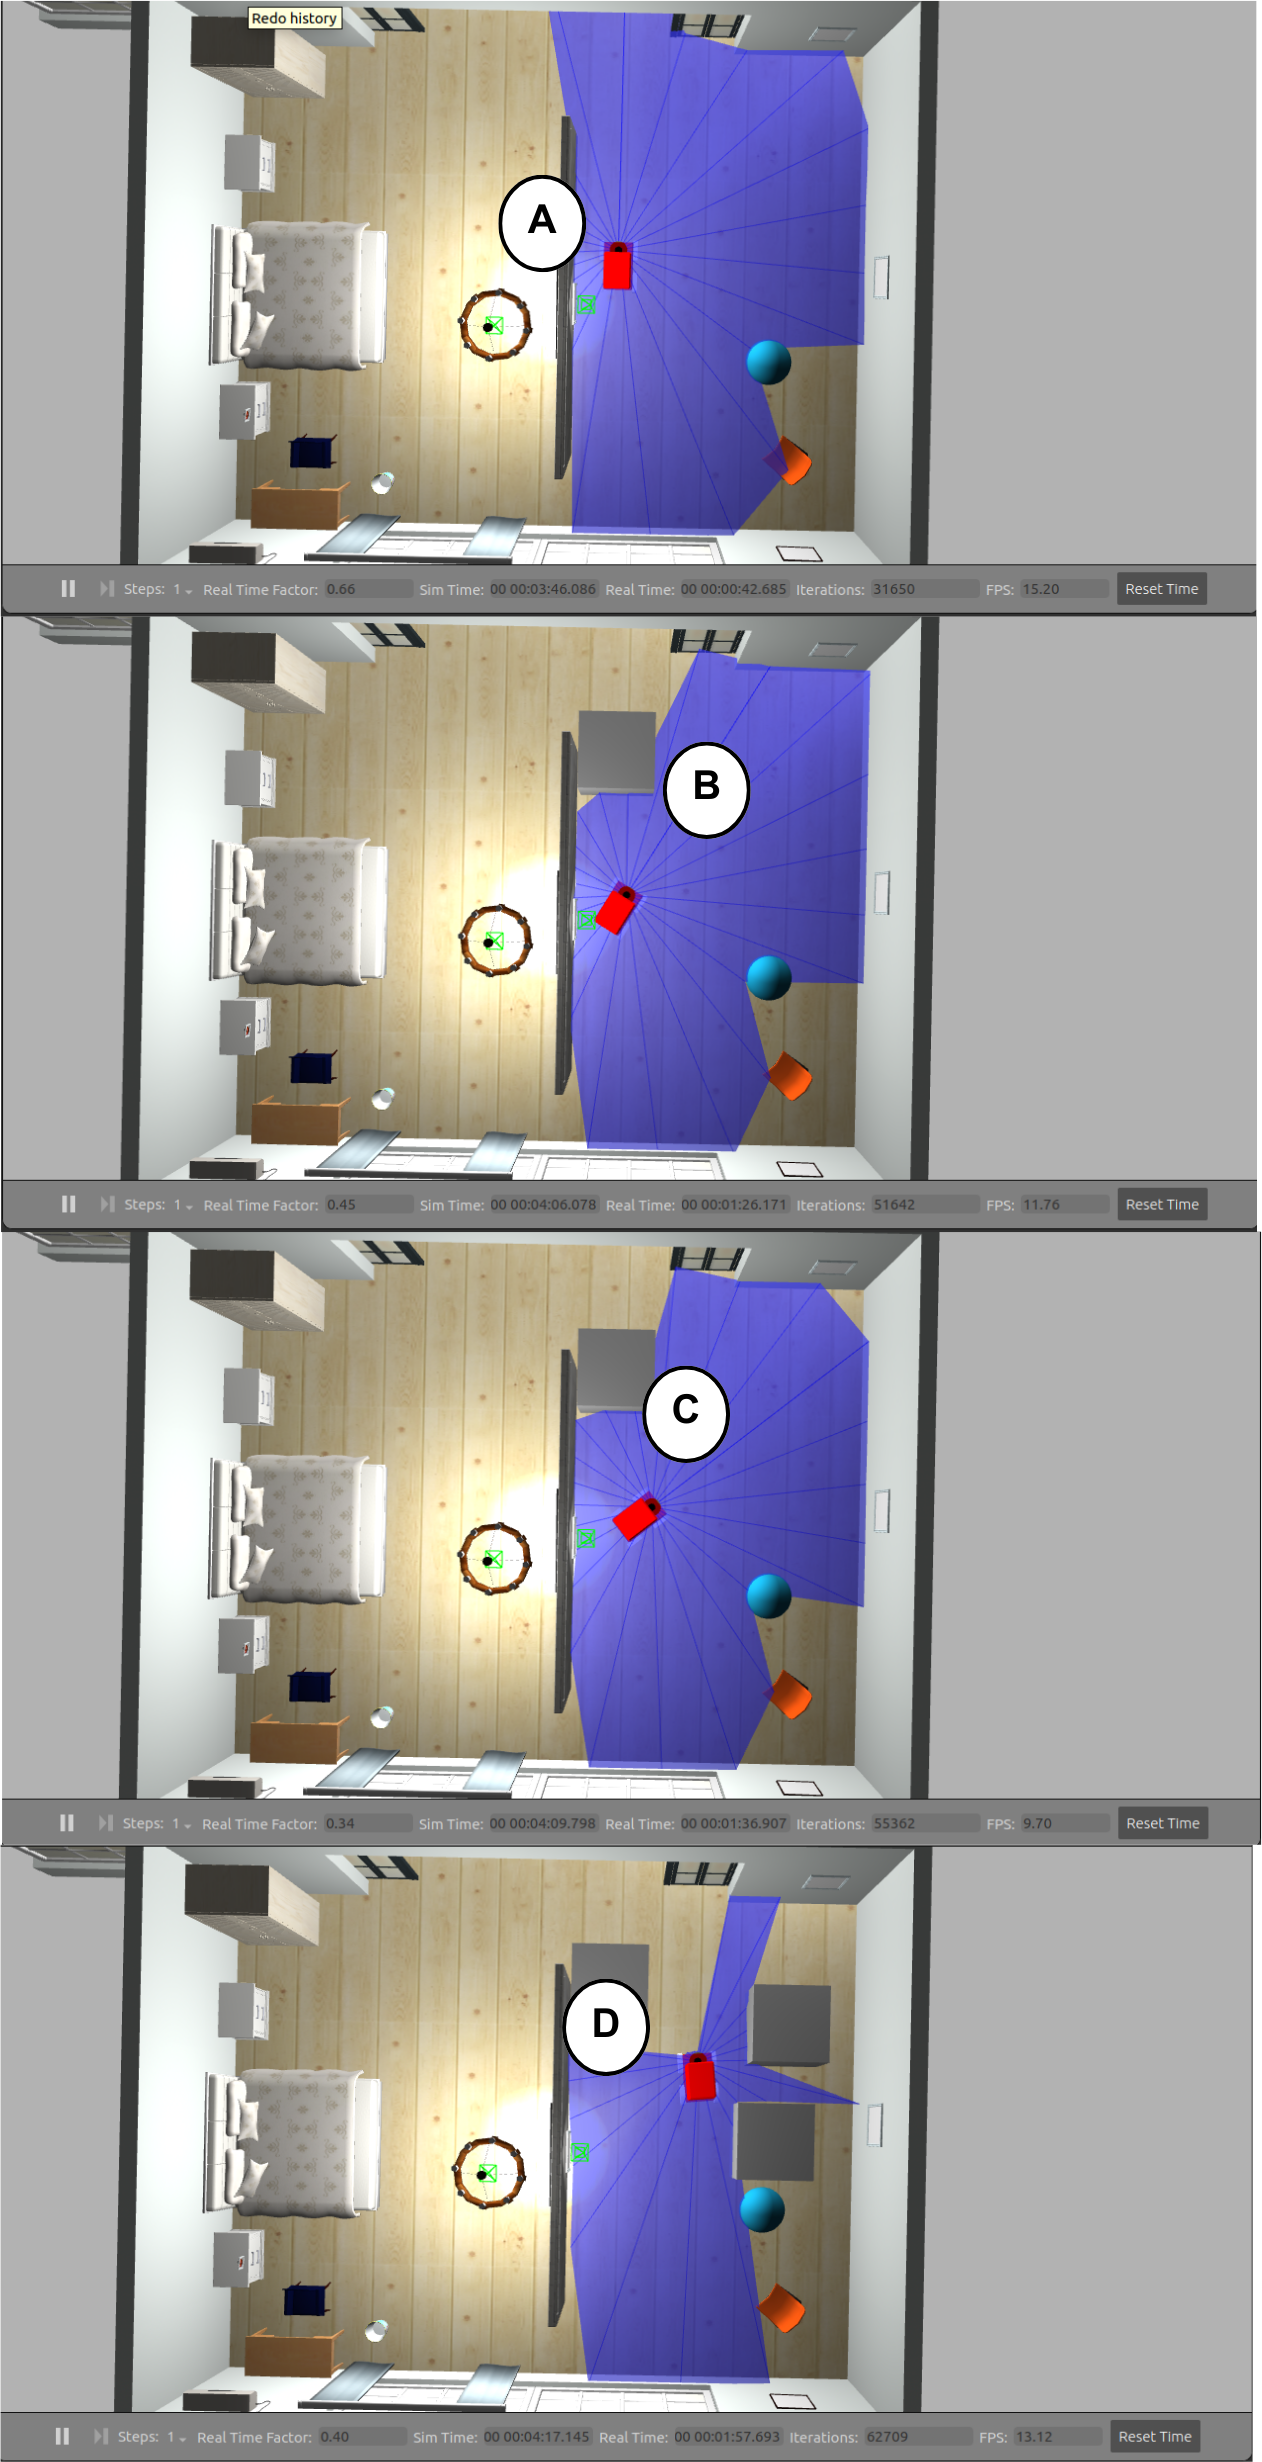
\includegraphics[scale=0.35]{ct01_1.png}
    \caption*{Fonte: Autora (2023).}
    \label{fig:ct01_1}
\end{figure}


\begin{figure}[H]
    \centering
    \caption{Captura da segunda repetição CT01}
    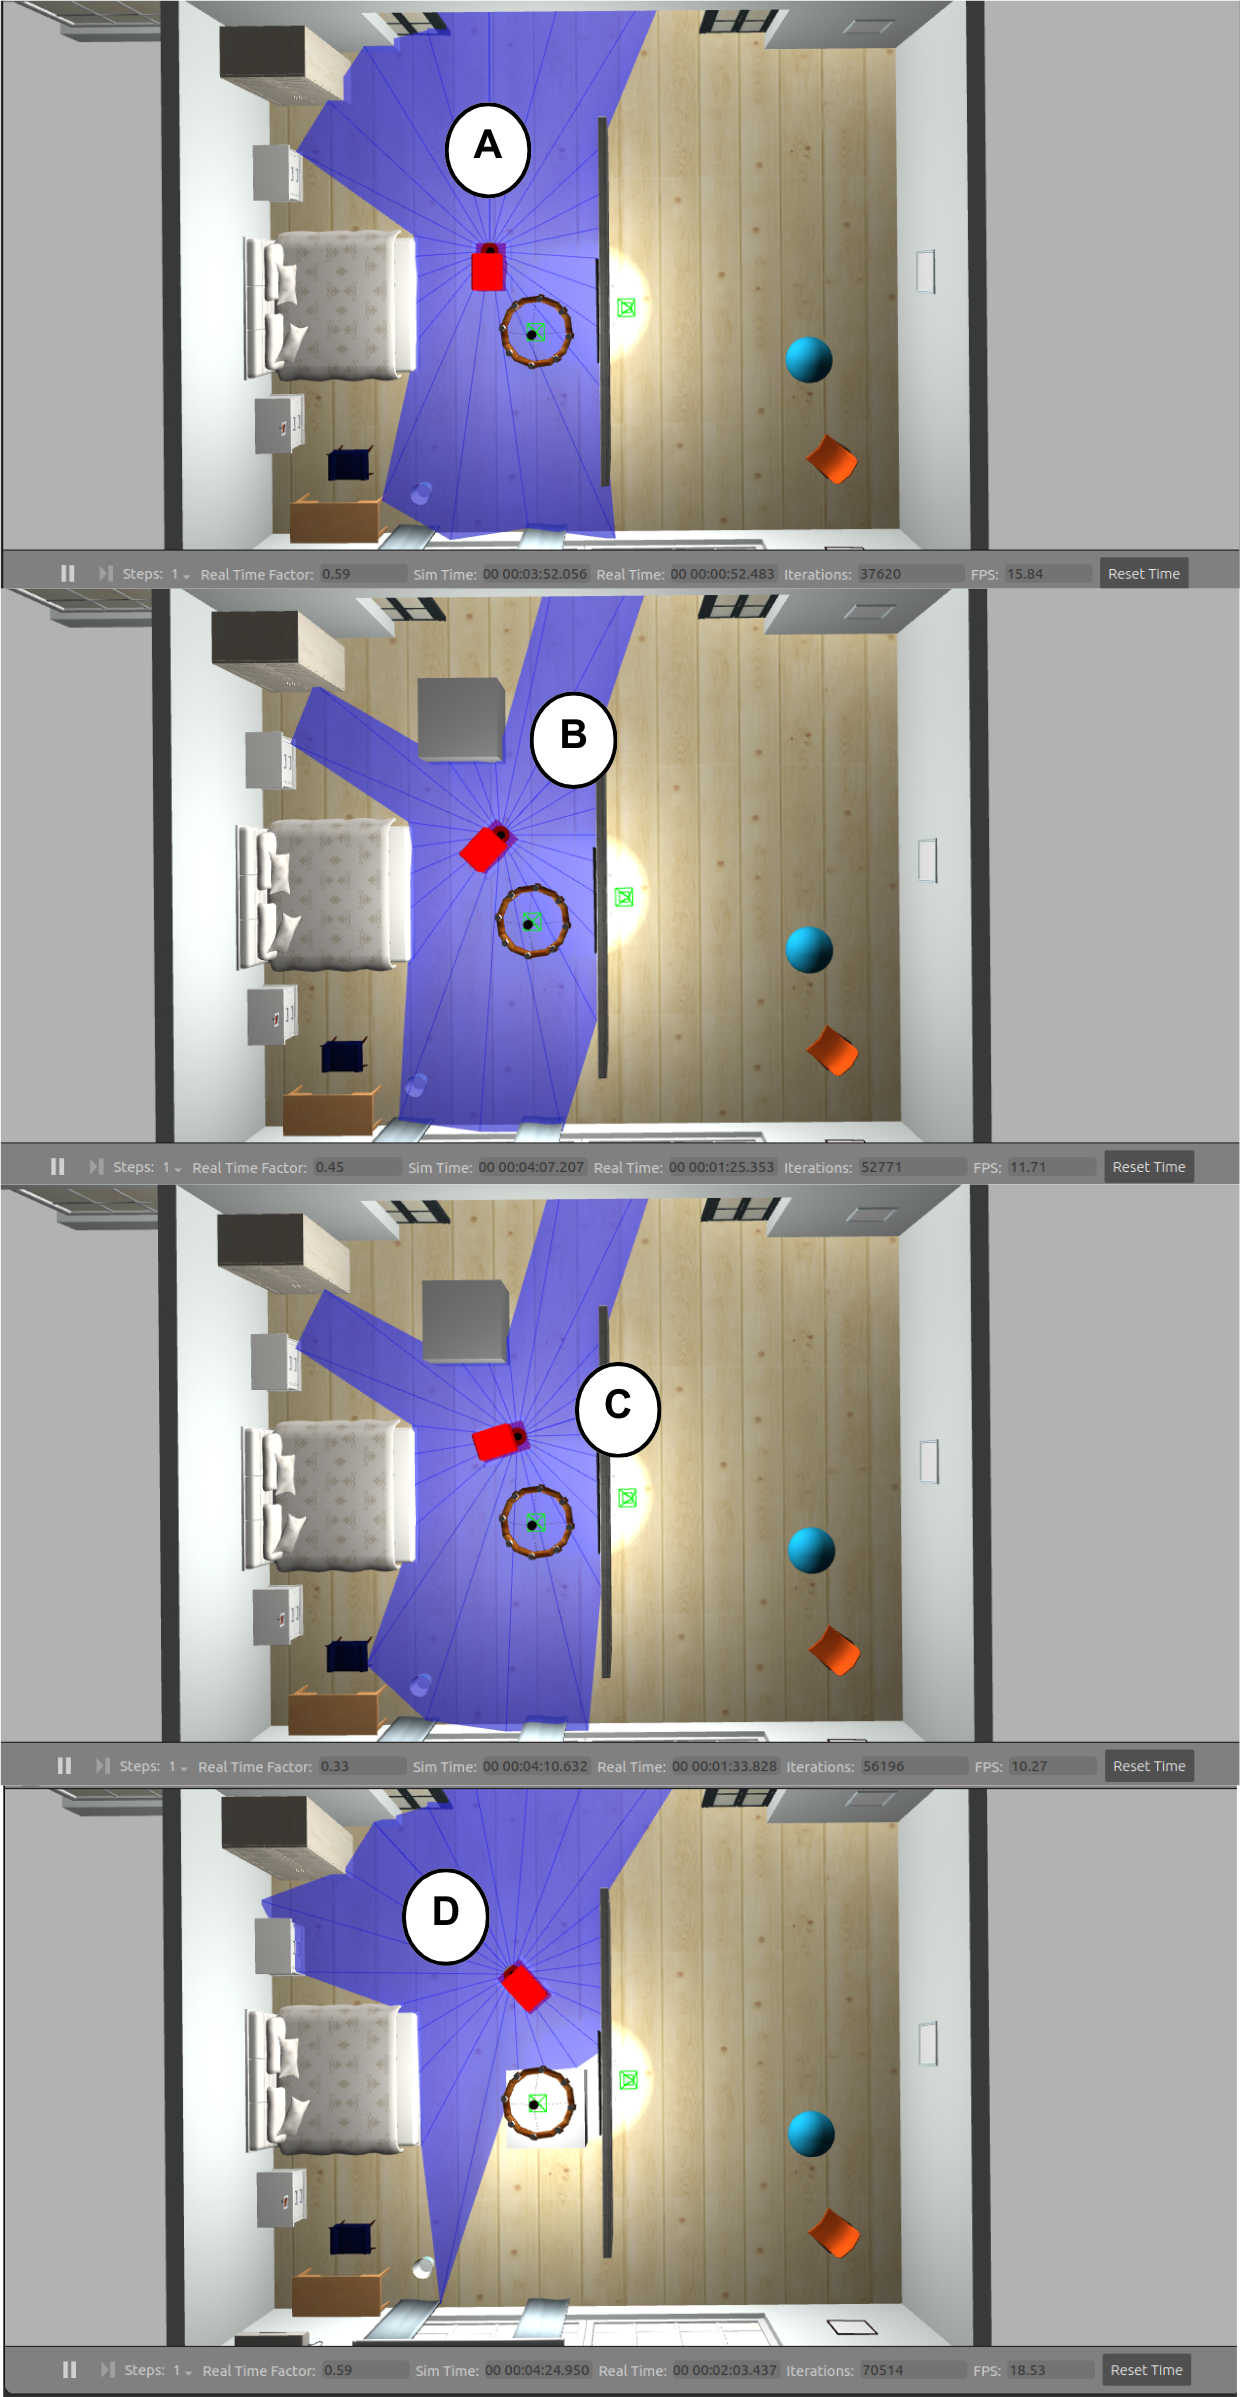
\includegraphics[scale=0.35]{ct01_2.png}
    \caption*{Fonte: Autora (2023).}
    \label{fig:ct01_2}
\end{figure}

\begin{figure}[H]
    \centering
    \caption{Captura da terceira repetição CT01}
    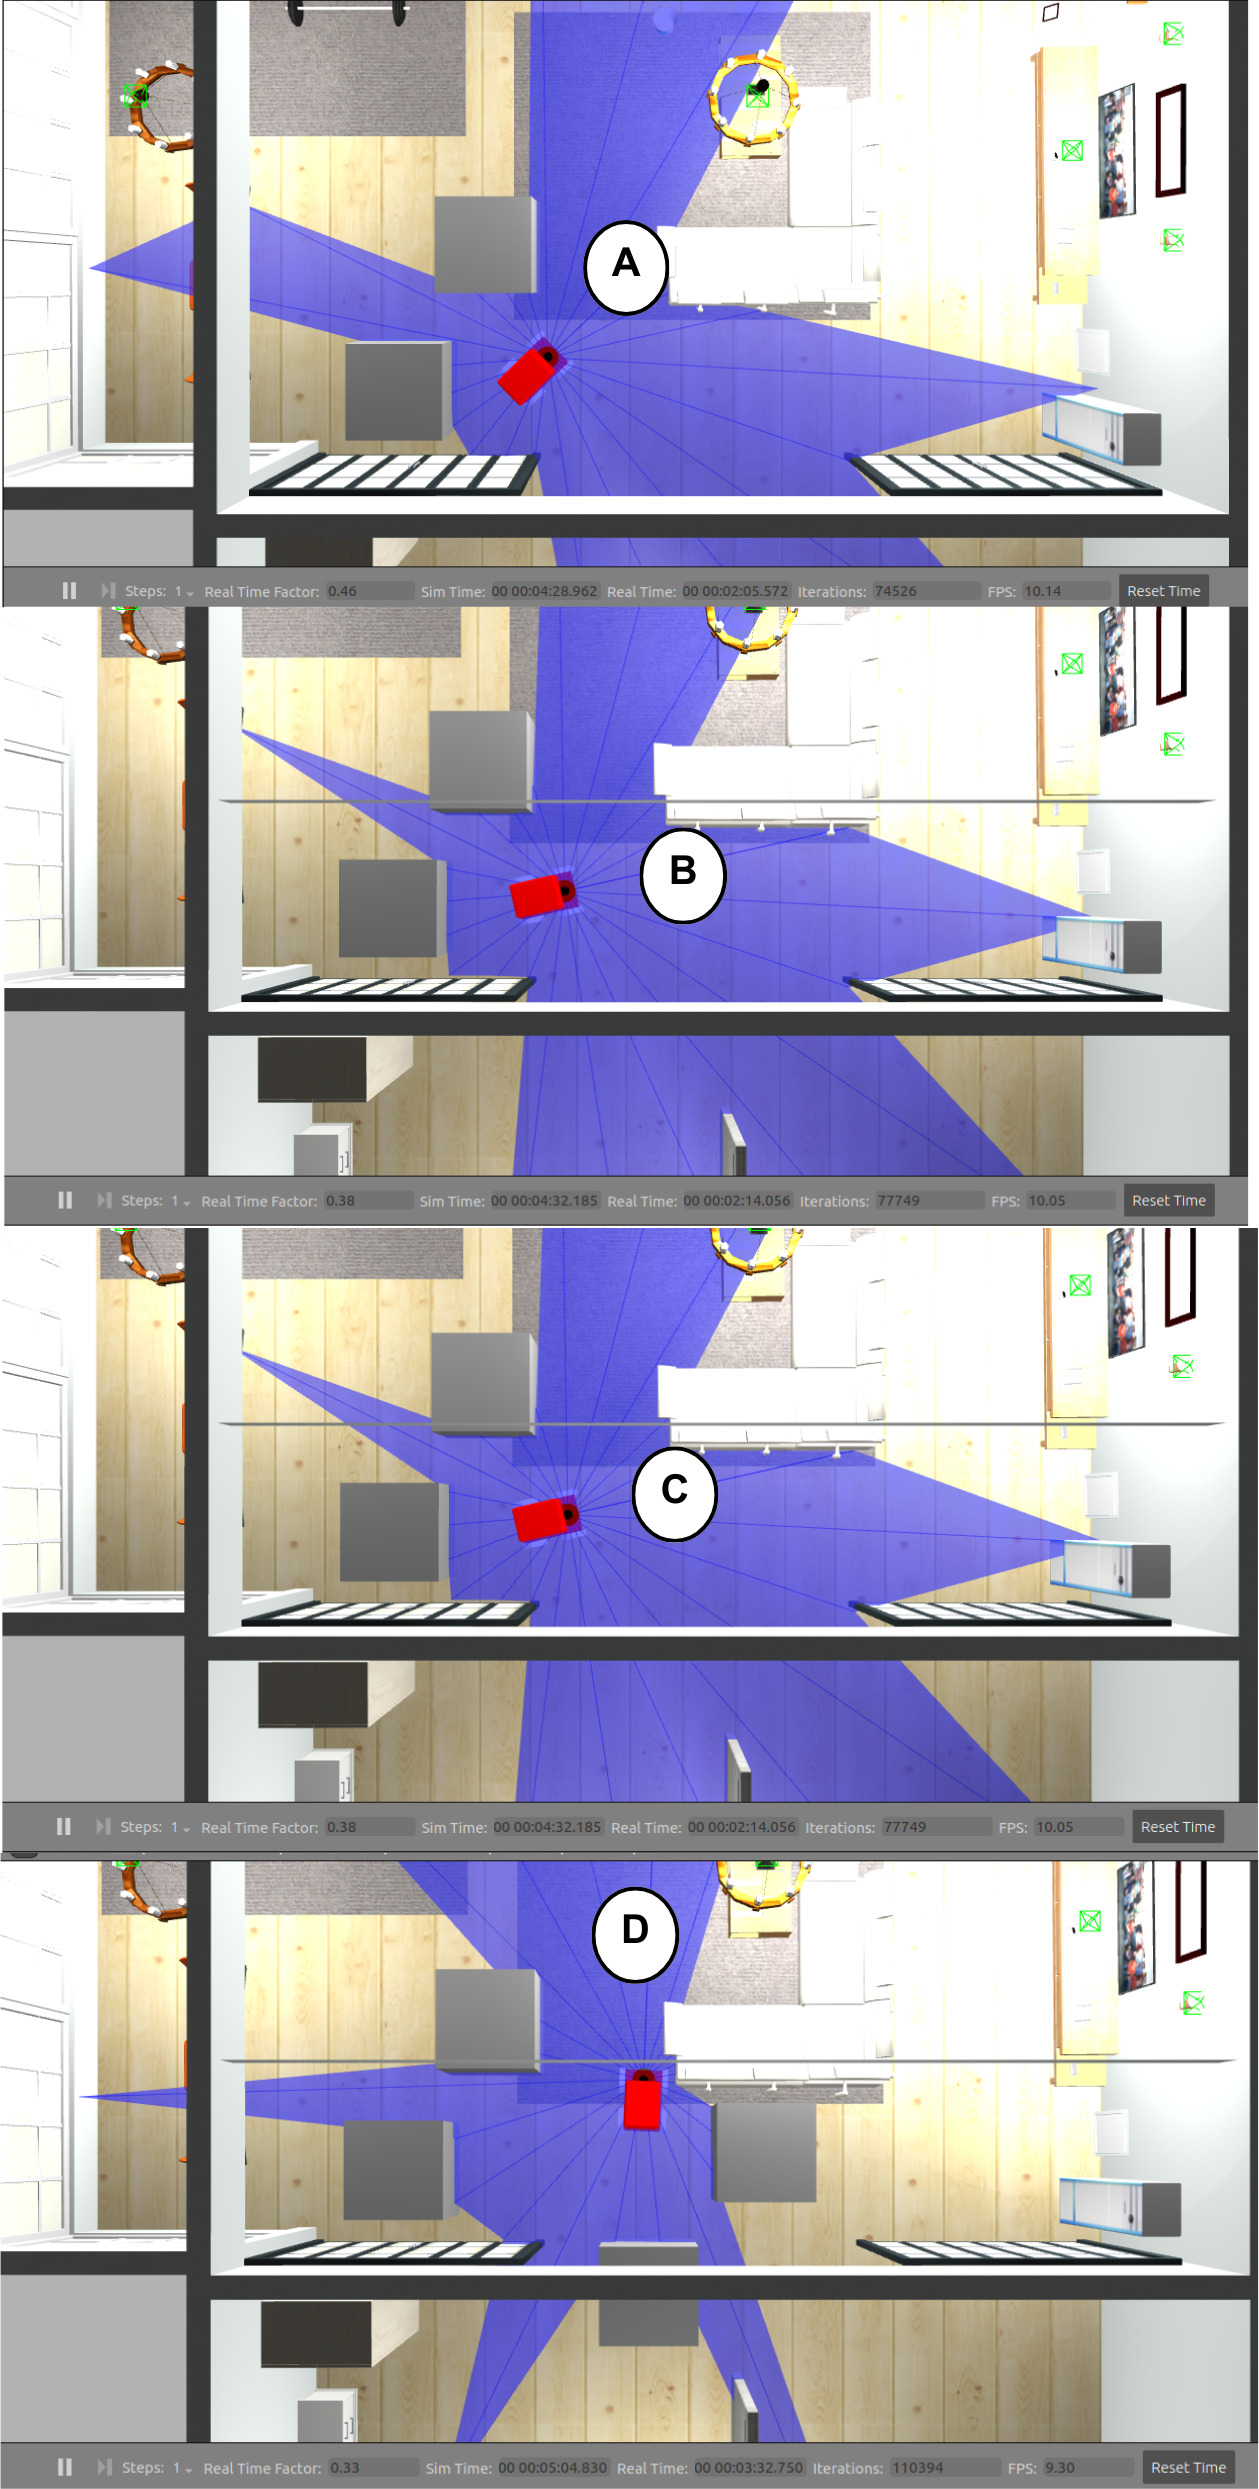
\includegraphics[scale=0.35]{ct01_3.png}
    \caption*{Fonte: Autora (2023).}
    \label{fig:ct01_3}
\end{figure}

\begin{figure}[H]
    \centering
    \caption{Captura da quarta repetição CT01}
    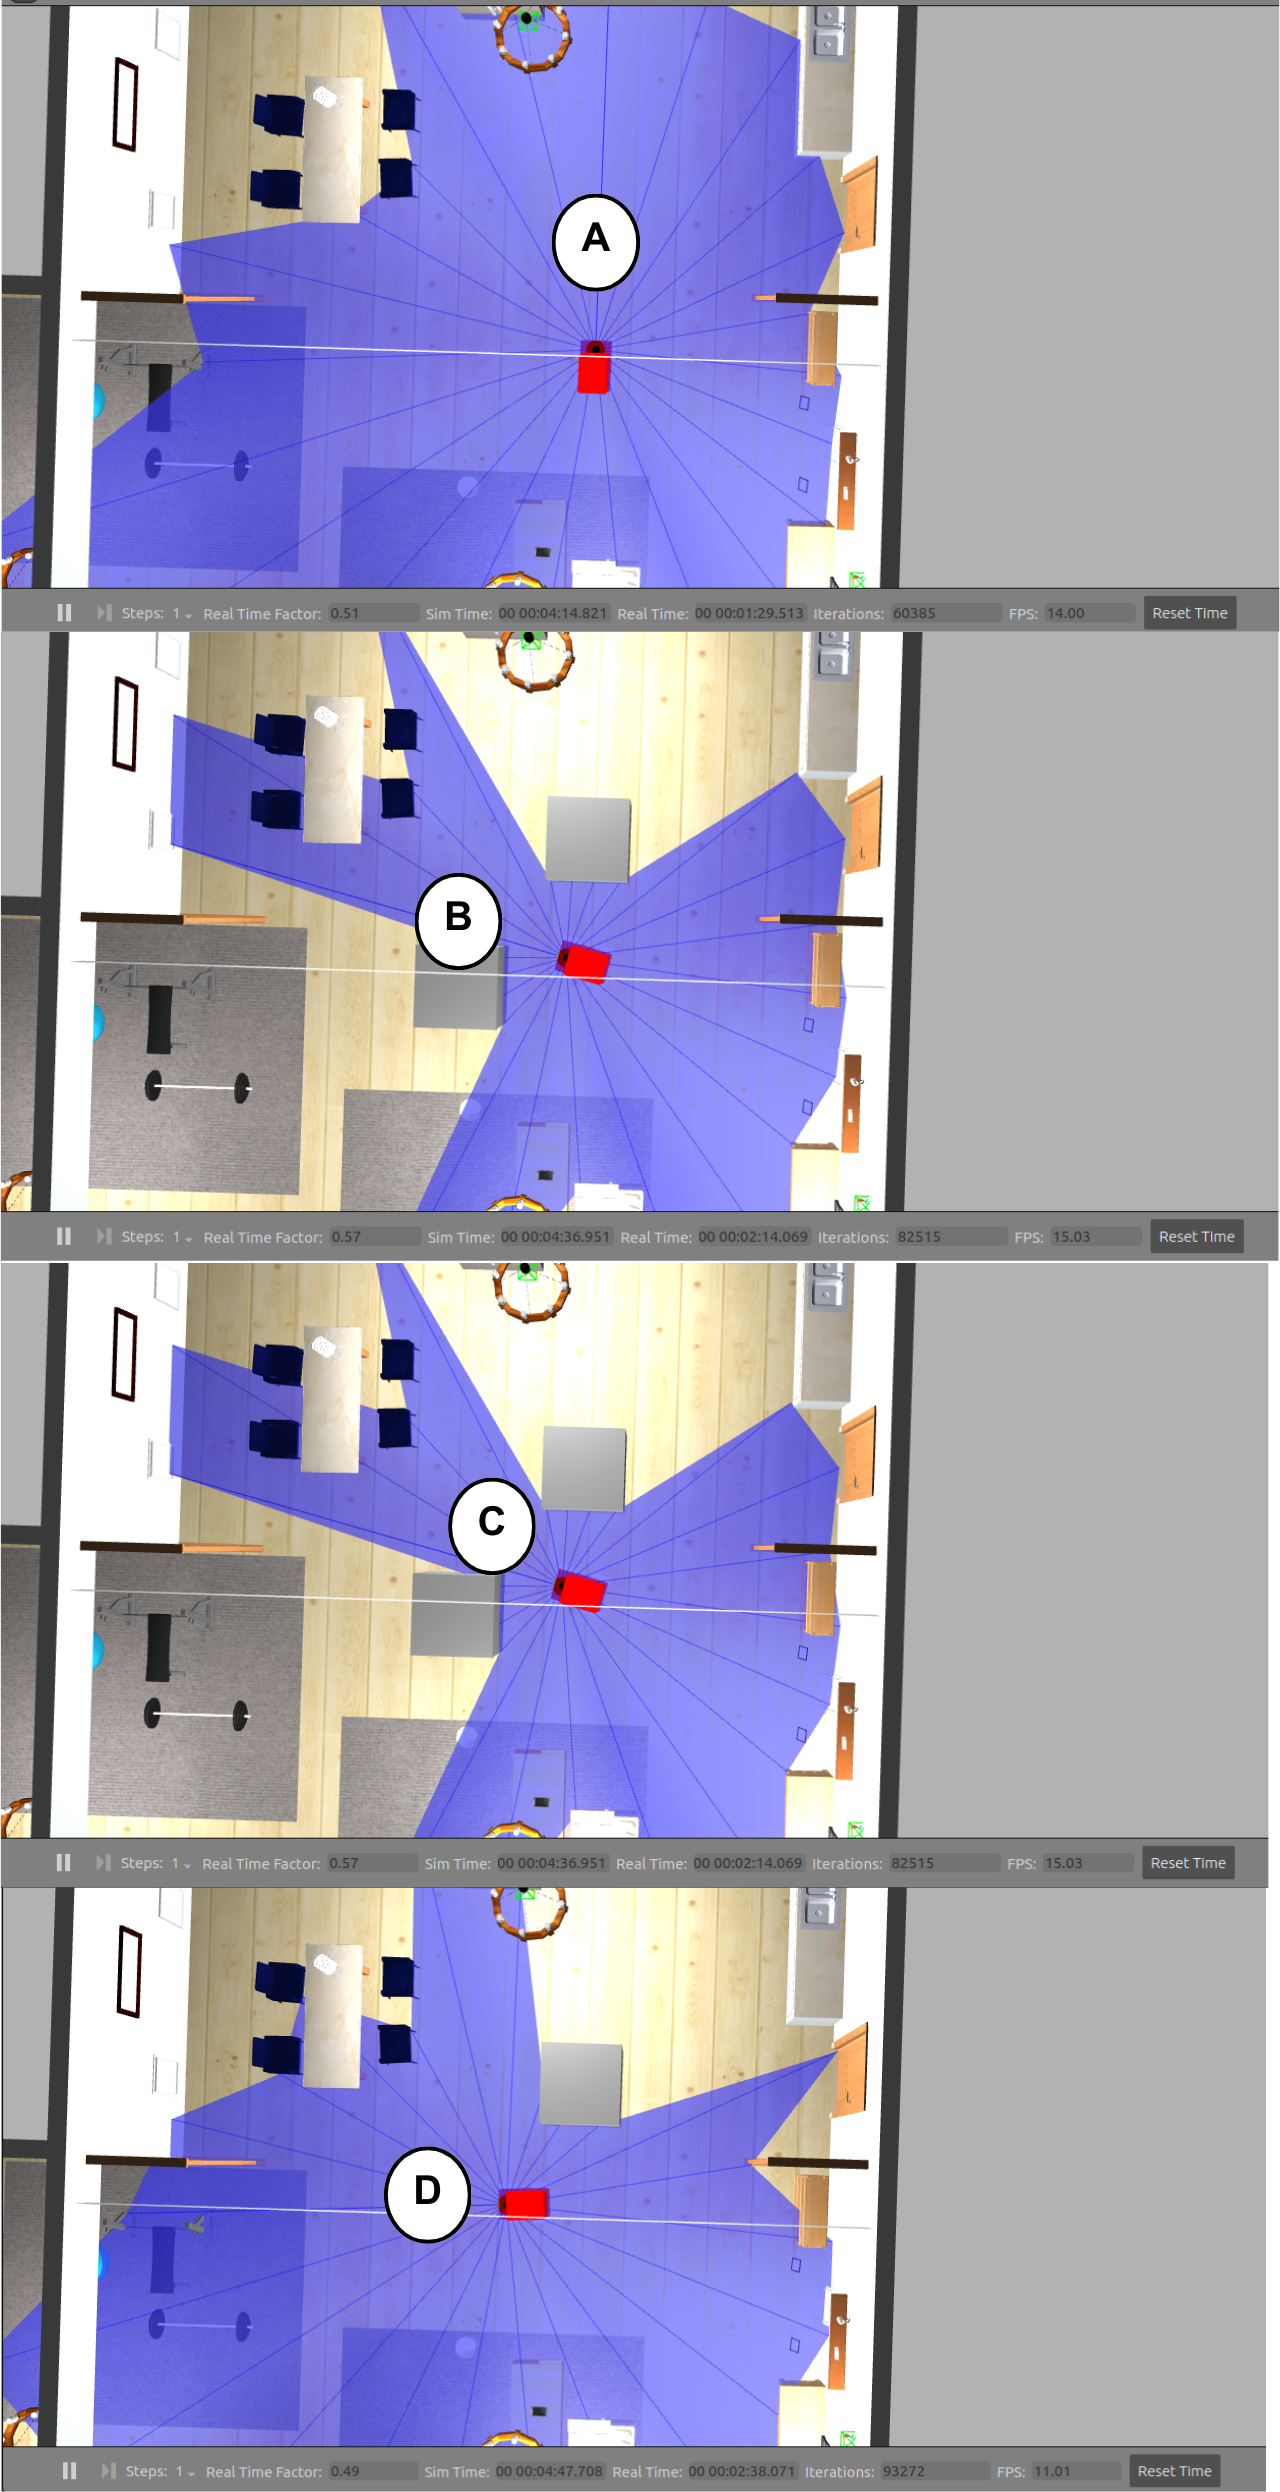
\includegraphics[scale=0.35]{ct01_4.png}
    \caption*{Fonte: Autora (2023).}
    \label{fig:ct01_4}
\end{figure}

\begin{figure}[H]
    \centering
    \caption{Captura da quinta repetição CT01}
    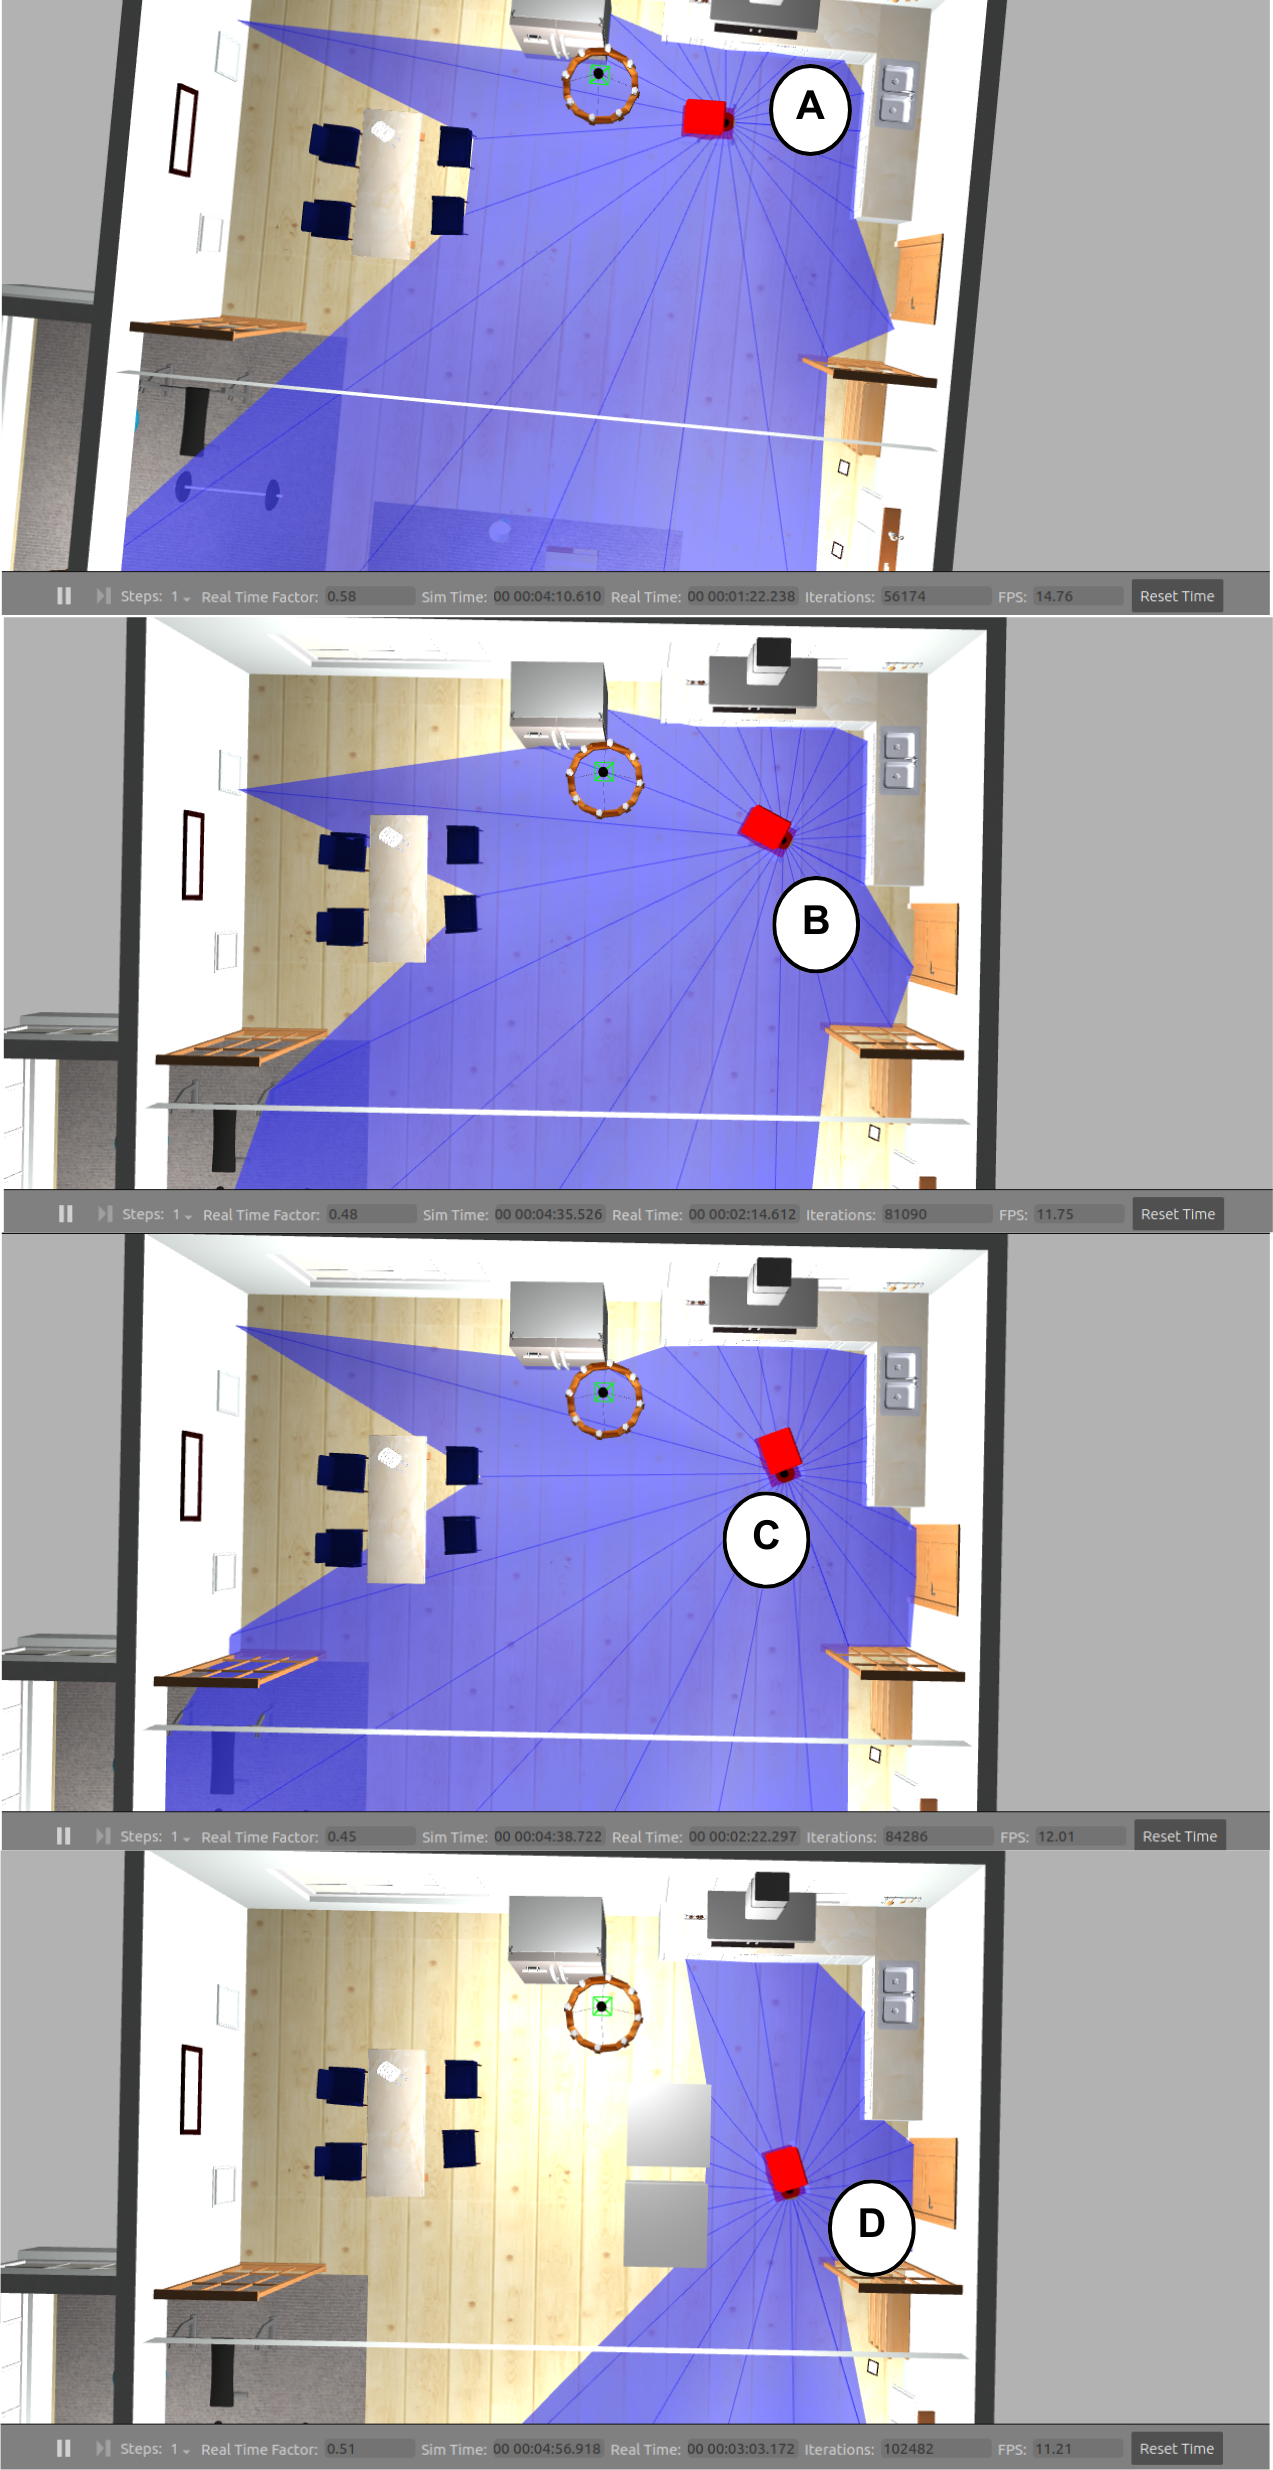
\includegraphics[scale=0.35]{ct01_5.png}
    \caption*{Fonte: Autora (2023).}
    \label{fig:ct01_5}
\end{figure}

\section{Caso de Teste CT02 Referente a RFS02}
O caso de teste CT02 teve o objetivo de identificar se o robô consegue se movimentar pelo ambiente sem colidir com nenhum obstáculo existente no seu caminho.  O caso de teste foi repetido cinco vezes com o robô em lugares distintos no ambiente. Entre os cinco testes, apenas um foi mal sucedido, visto que o robô se encontrava em um local estreito e não conseguiu continuar a trajetória. Todos os resultados podem ser visualizados na Tabela~\ref{tab:acertosct02}. Além disso, a seguir podem ser encontradas as capturas para cada repetição (Figura~\ref{fig:ct02_1}, Figura~\ref{fig:ct02_2}, Figura~\ref{fig:ct02_3}, Figura~\ref{fig:ct02_4}, Figura~\ref{fig:ct02_5}).


\begin{table}[H]
\centering
\caption{Resultados das repetições CT02}
\label{tab:acertosct02}
\resizebox{\textwidth}{!}{%
\begin{tabular}{l|c}
                              & \multicolumn{1}{l}{\textbf{Resultados CT02}} \\ \hline
\textbf{Teste 1}              & Bem-sucedido                                 \\
\textbf{Teste 2}              & Bem-sucedido                                 \\
\textbf{Teste 3}              & Bem-sucedido                                 \\
\textbf{Teste 4}              & Mal-sucedido                                 \\
\textbf{Teste 5}              & Bem-sucedido                                 \\
\textbf{Total de acertos (\%)} & \textbf{80}                                  \\ \hline
\end{tabular}%
}
\caption*{Fonte: Autora (2023).}
\end{table}

\begin{figure}[H]
    \centering
    \caption{Captura da primeira repetição CT02}
    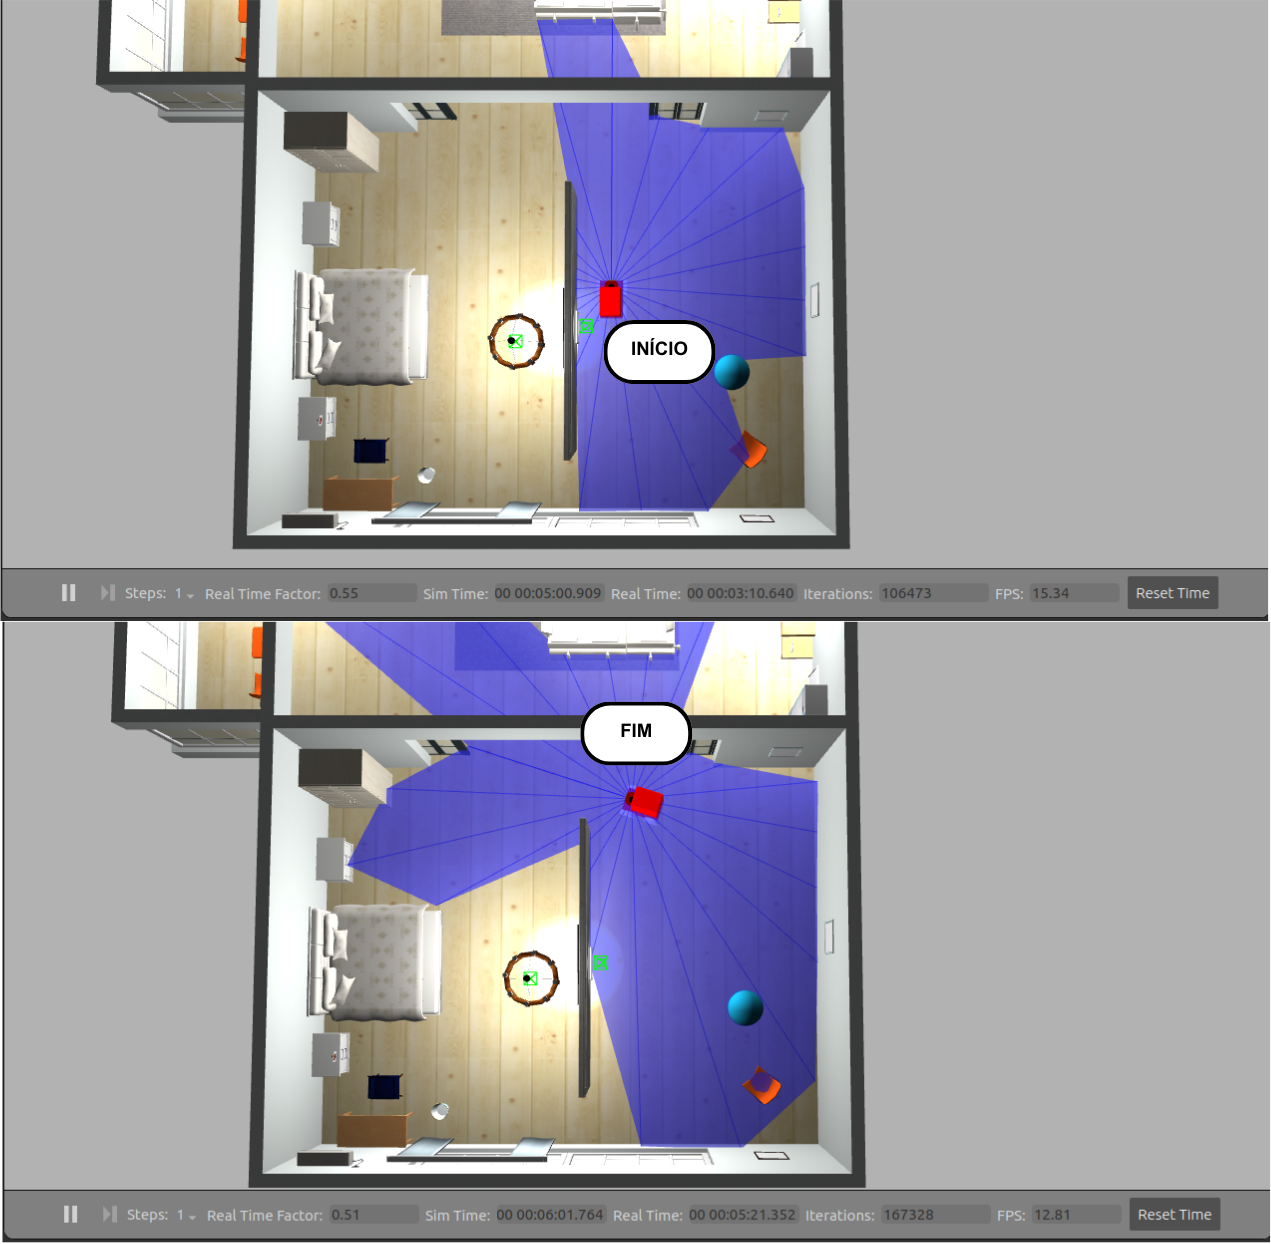
\includegraphics[scale=0.5]{ct02_1.png}
    \caption*{Fonte: Autora (2023).}
    \label{fig:ct02_1}
\end{figure}


\begin{figure}[H]
    \centering
    \caption{Captura da segunda repetição CT02}
    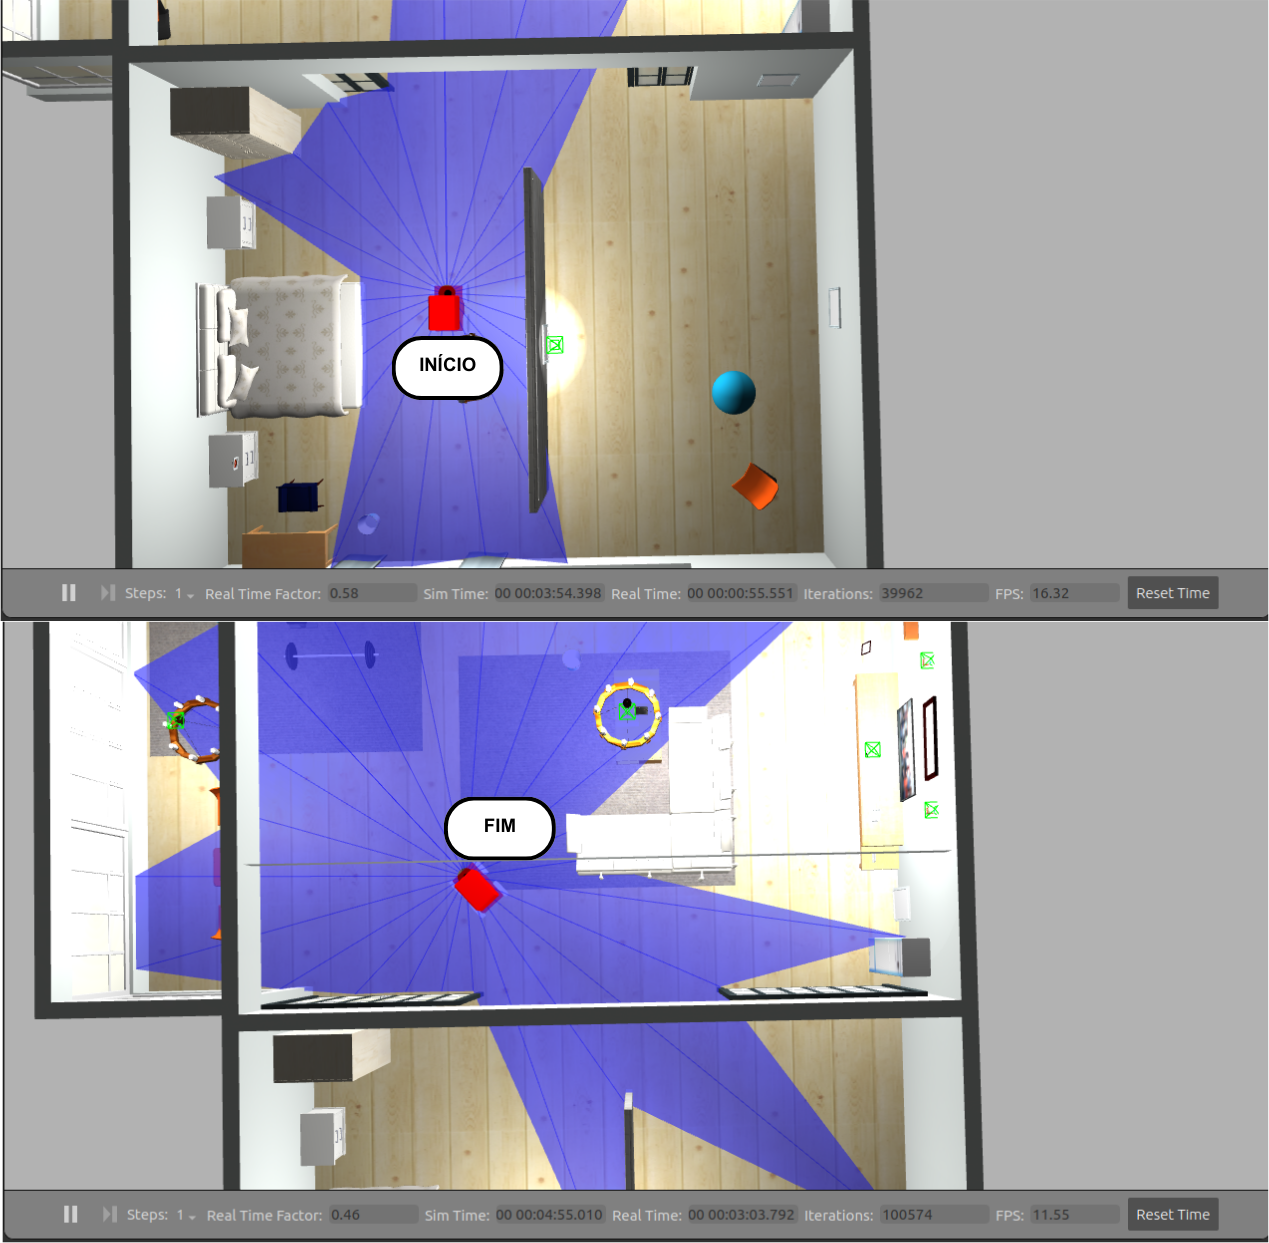
\includegraphics[scale=0.5]{ct02_2.png}
    \caption*{Fonte: Autora (2023).}
    \label{fig:ct02_2}
\end{figure}

\begin{figure}[H]
    \centering
    \caption{Captura da terceira repetição CT02}
    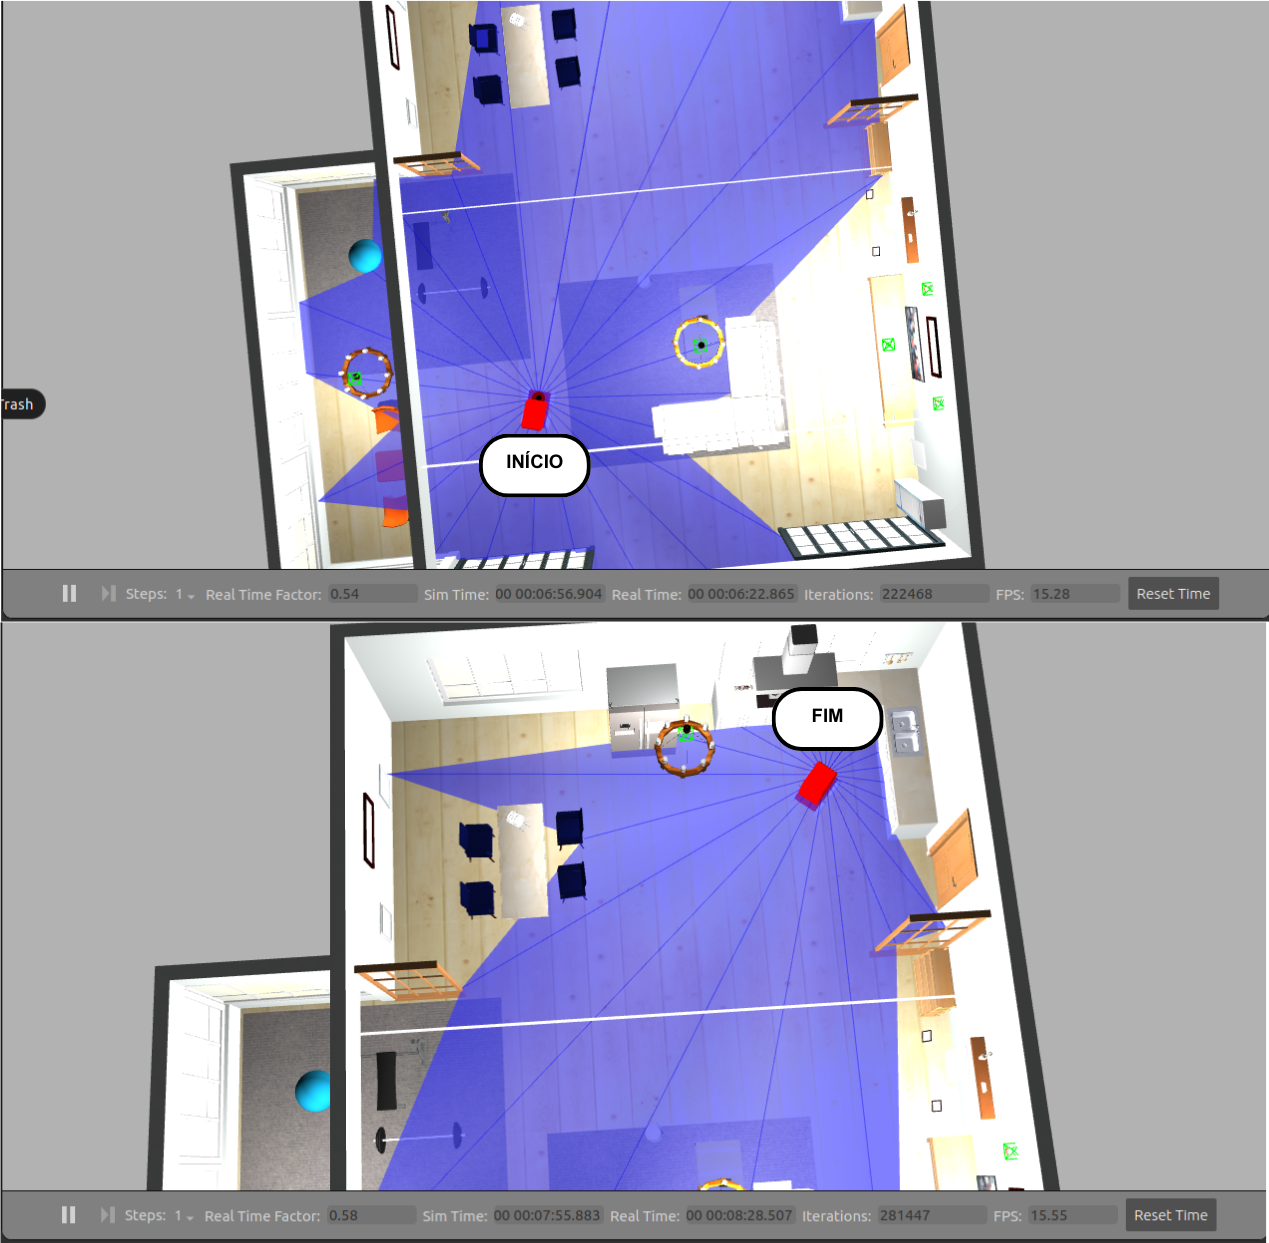
\includegraphics[scale=0.5]{ct02_3.png}
    \caption*{Fonte: Autora (2023).}
    \label{fig:ct02_3}
\end{figure}

\begin{figure}[H]
    \centering
    \caption{Captura da quarta repetição CT02}
    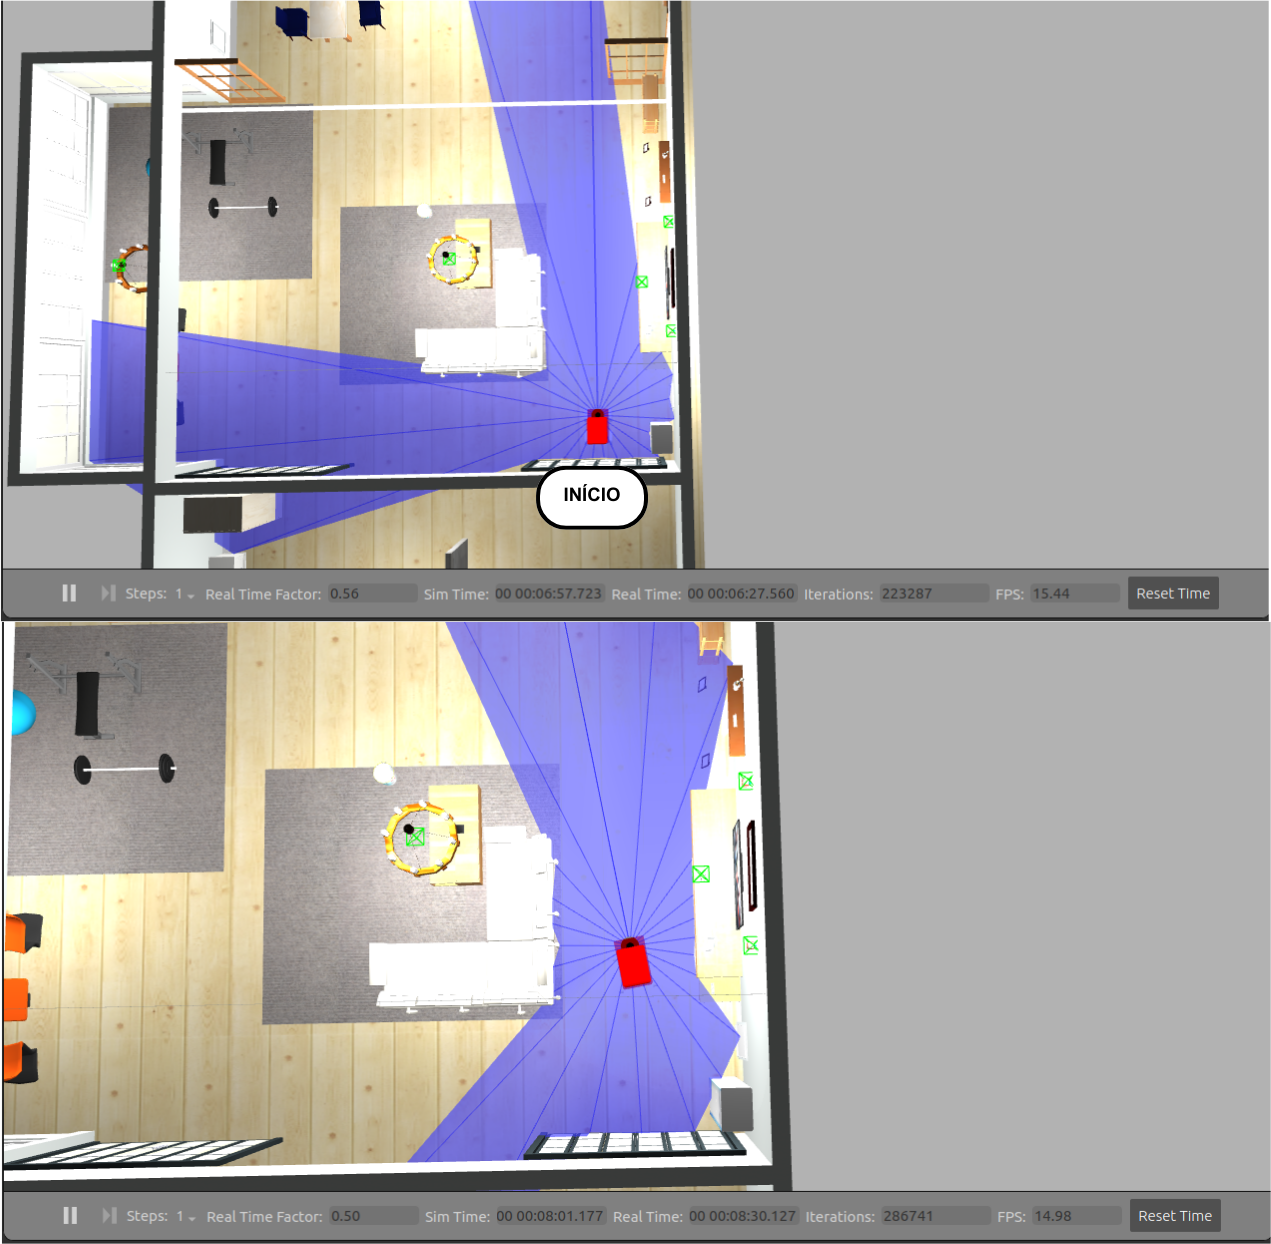
\includegraphics[scale=0.5]{ct02_4.png}
    \caption*{Fonte: Autora (2023).}
    \label{fig:ct02_4}
\end{figure}

\begin{figure}[H]
    \centering
    \caption{Captura da quinta repetição CT02}
    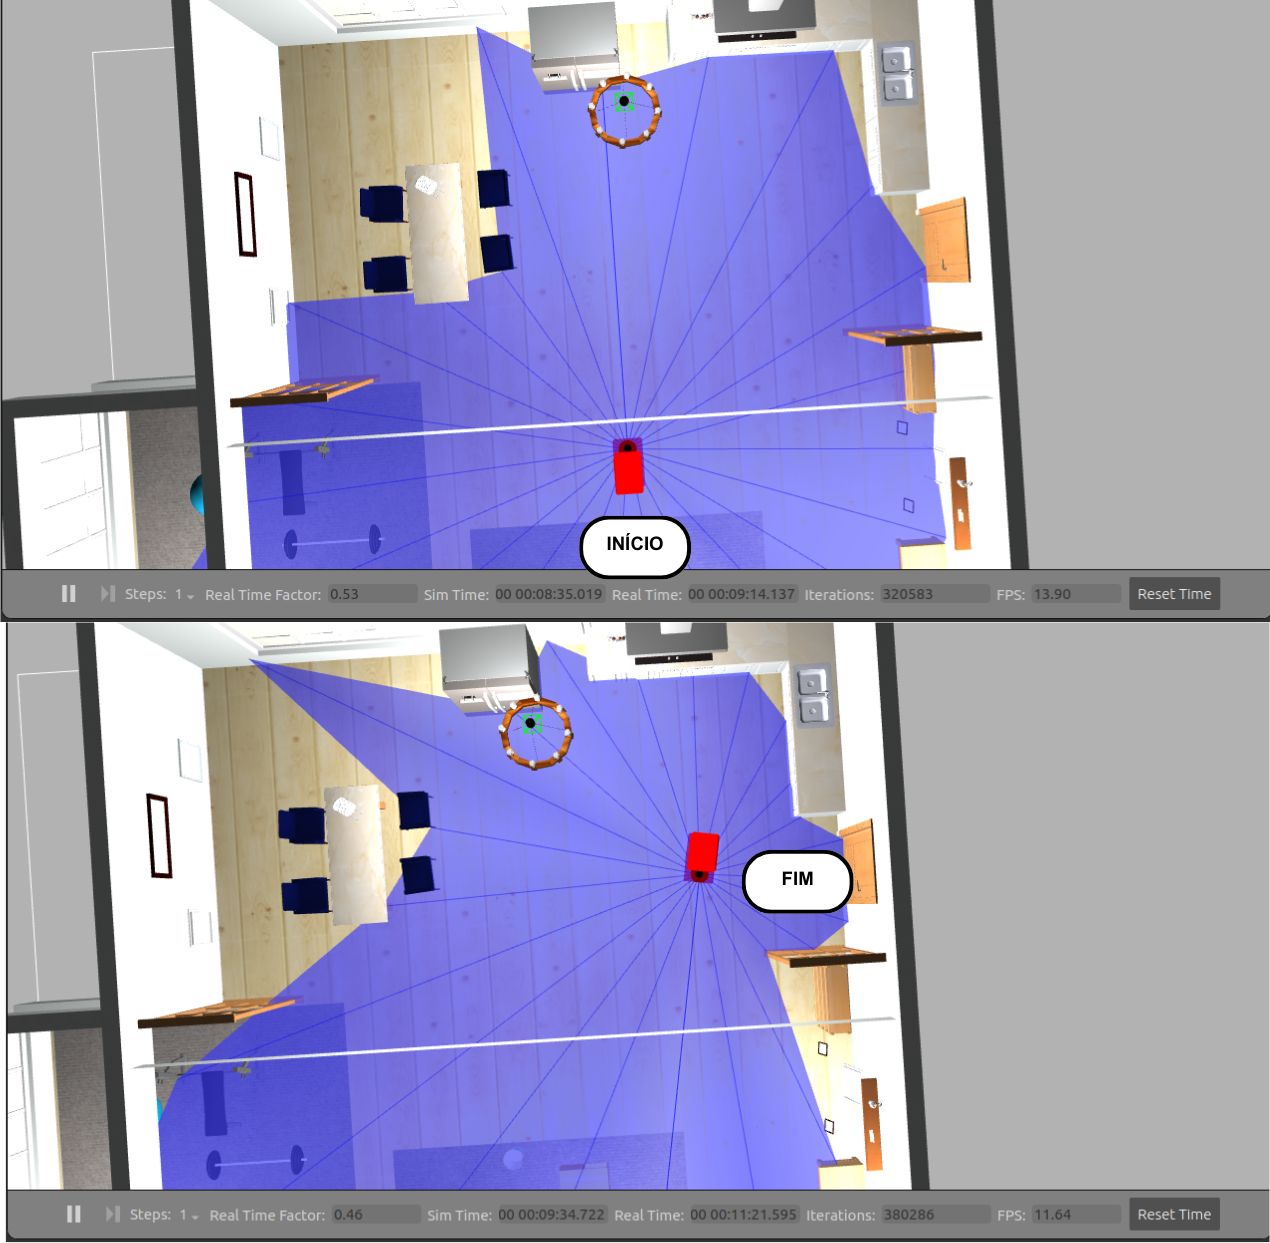
\includegraphics[scale=0.5]{ct02_5.png}
    \caption*{Fonte: Autora (2023).}
    \label{fig:ct02_5}
\end{figure}

\section{Caso de Teste CT03 Referente a RNFS01}
O caso de teste CT03 visou validar a locomoção do robô em superfície de piso liso e com tapete. O caso de teste foi repetido cinco vezes com o robô em lugares distintos no ambiente. Todos os cinco testes foram bem sucedidos. Todos os resultados podem ser visualizados na Tabela~\ref{tab:acertosct03}. Além disso, a seguir podem ser encontradas as capturas para cada repetição (Figura~\ref{fig:ct03_1}, Figura~\ref{fig:ct03_2}, Figura~\ref{fig:ct03_3}, Figura~\ref{fig:ct03_4}, Figura~\ref{fig:ct03_5}).


\begin{table}[H]
\centering
\caption{Resultados das Repetições CT03}
\label{tab:acertosct03}
\resizebox{\textwidth}{!}{%
\begin{tabular}{l|c}
                              & \multicolumn{1}{l}{\textbf{Resultados CT03}} \\ \hline
\textbf{Teste 1}              & Bem-sucedido                                 \\
\textbf{Teste 2}              & Bem-sucedido                                 \\
\textbf{Teste 3}              & Bem-sucedido                                 \\
\textbf{Teste 4}              & Bem-sucedido                                 \\
\textbf{Teste 5}              & Bem-sucedido                                 \\
\textbf{Total de acertos (\%)} & \textbf{100}                                  \\ \hline
\end{tabular}%
}
\caption*{Fonte: Autora (2023).}
\end{table}

\begin{figure}[H]
    \centering
    \caption{Captura da primeira repetição CT03}
    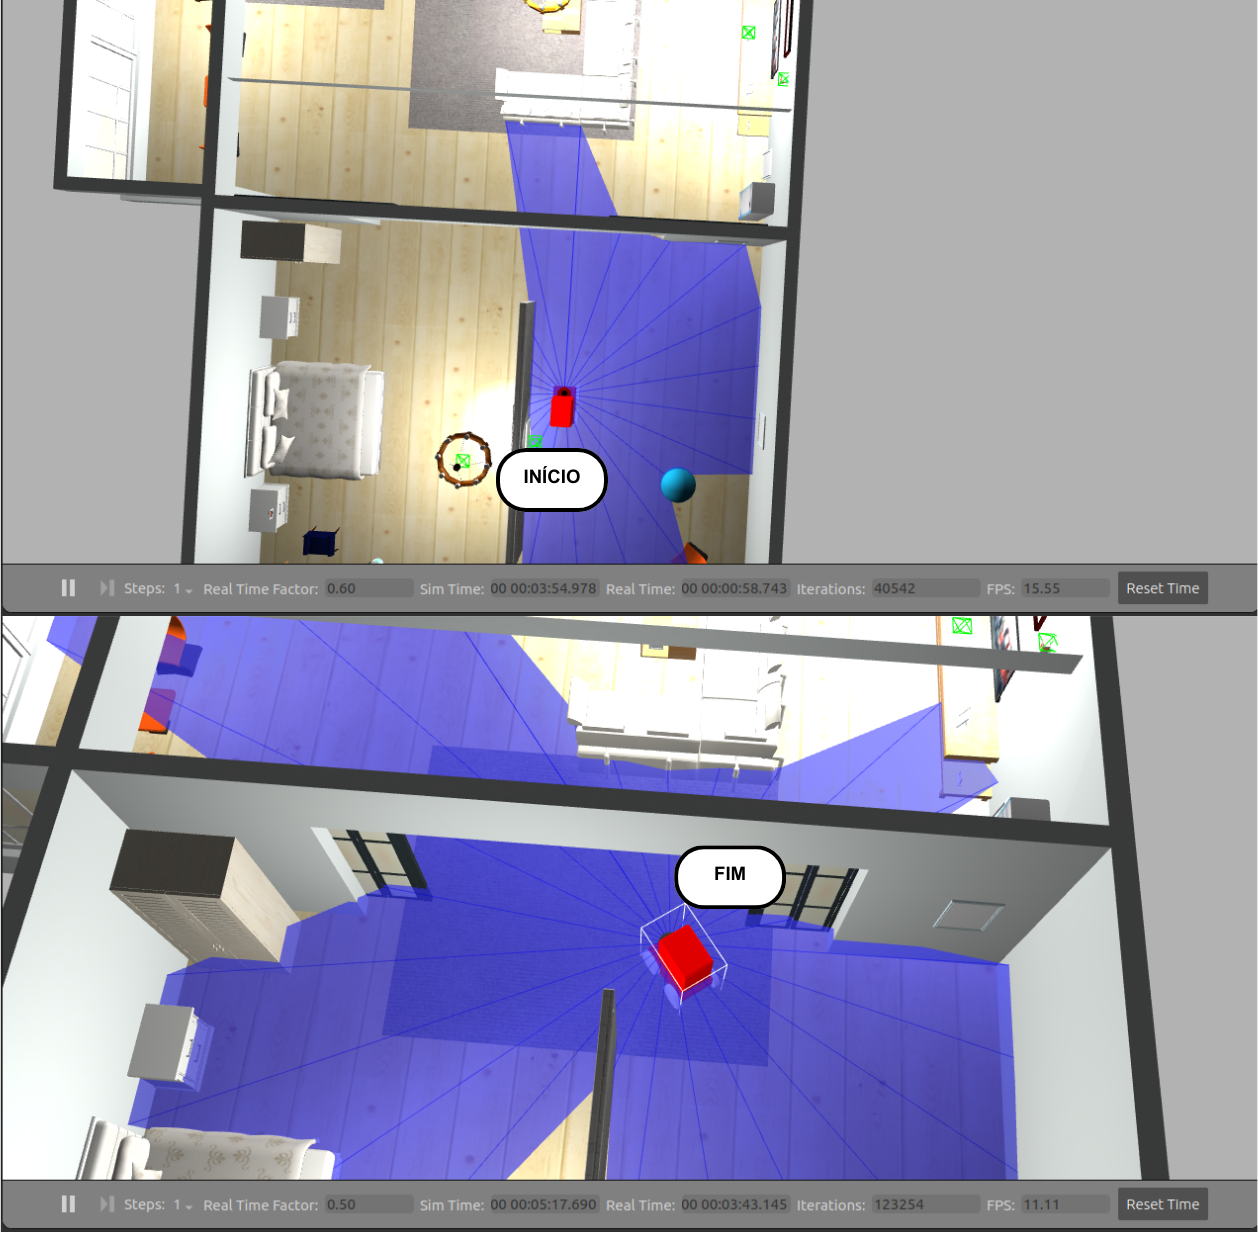
\includegraphics[scale=0.5]{ct03_1.png}
    \caption*{Fonte: Autora (2023).}
    \label{fig:ct03_1}
\end{figure}


\begin{figure}[H]
    \centering
    \caption{Captura da segunda repetição CT03}
    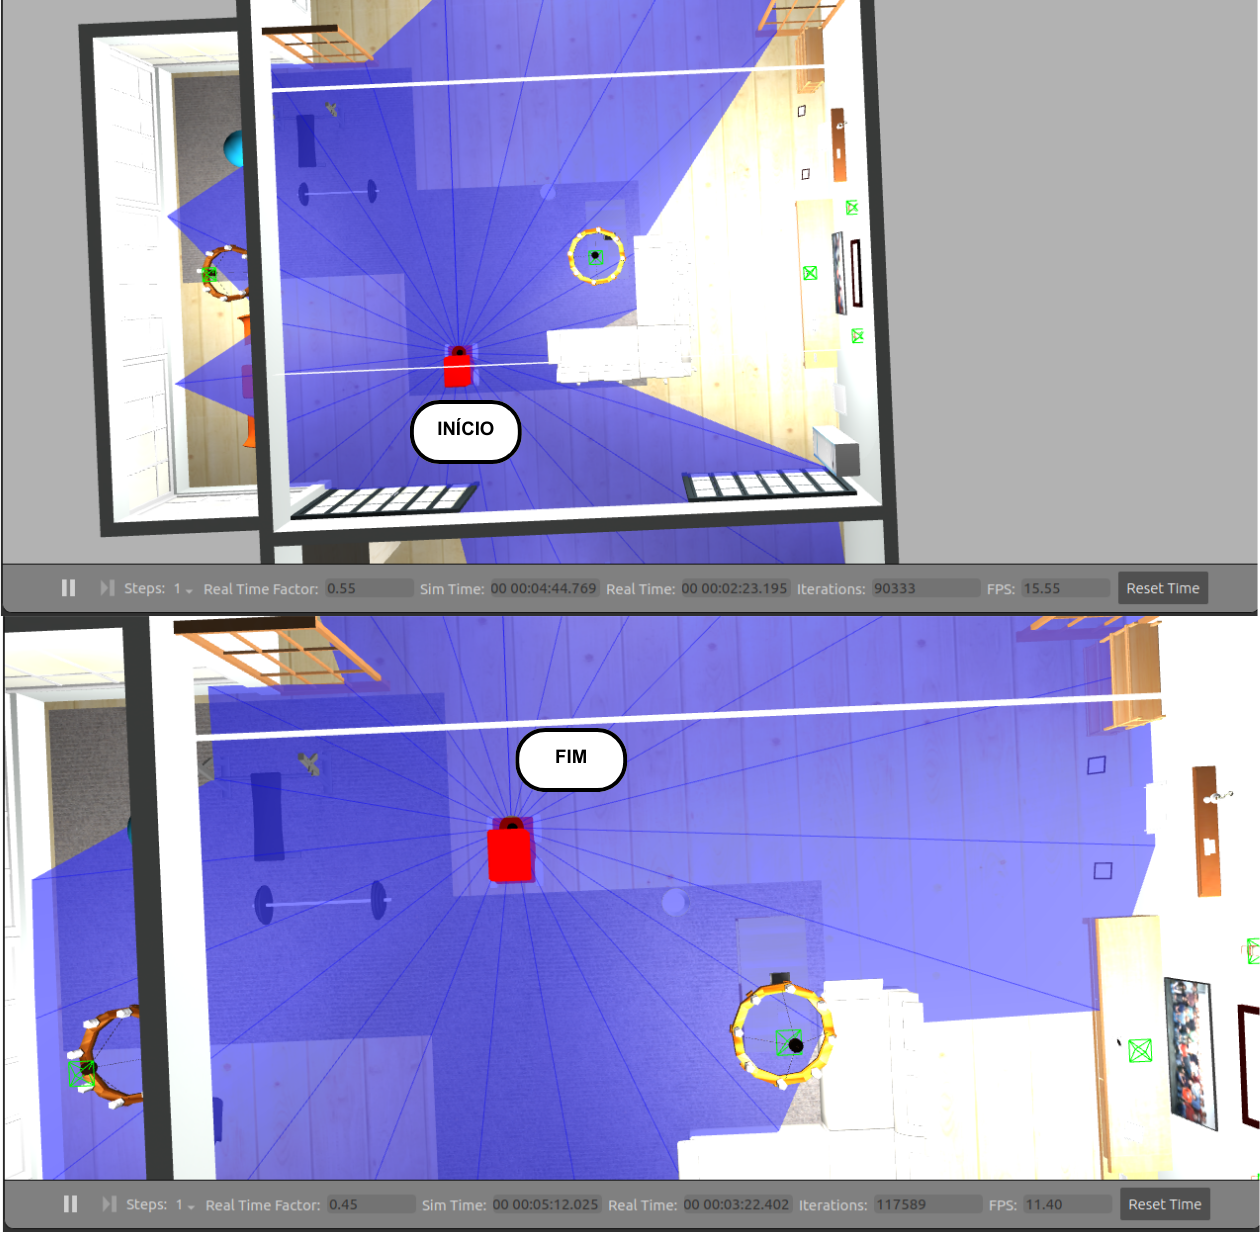
\includegraphics[scale=0.5]{ct03_2.png}
    \caption*{Fonte: Autora (2023).}
    \label{fig:ct03_2}
\end{figure}

\begin{figure}[H]
    \centering
    \caption{Captura da terceira repetição CT03}
    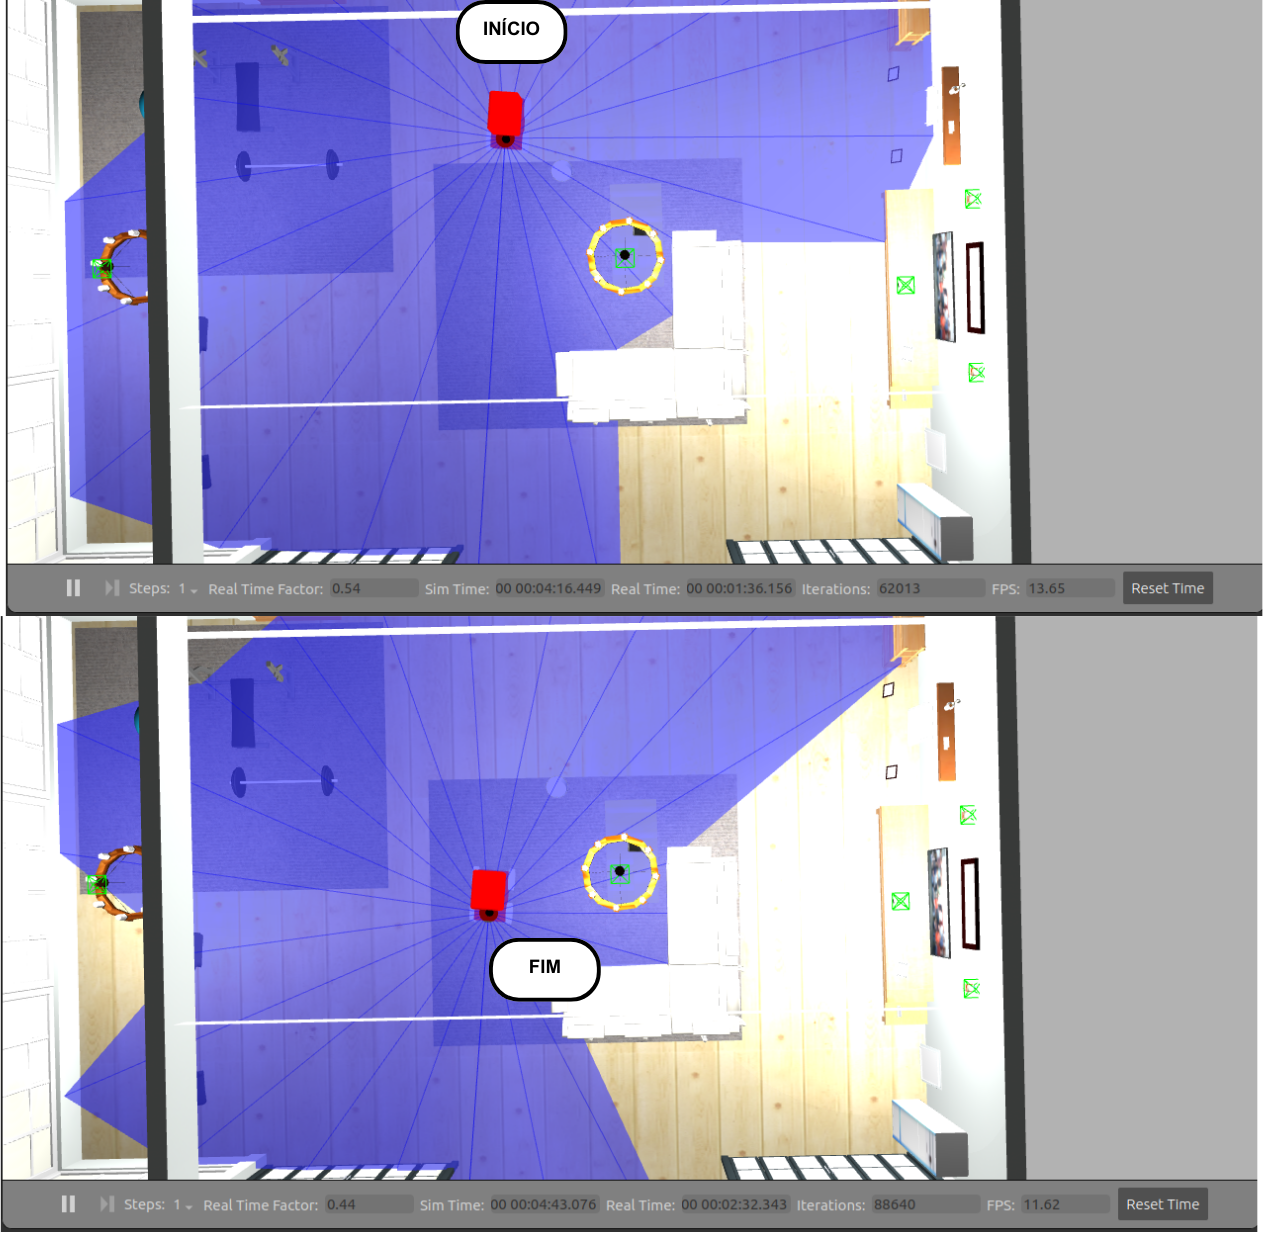
\includegraphics[scale=0.5]{ct03_3.png}
    \caption*{Fonte: Autora (2023).}
    \label{fig:ct03_3}
\end{figure}

\begin{figure}[H]
    \centering
    \caption{Captura da quarta repetição CT03}
    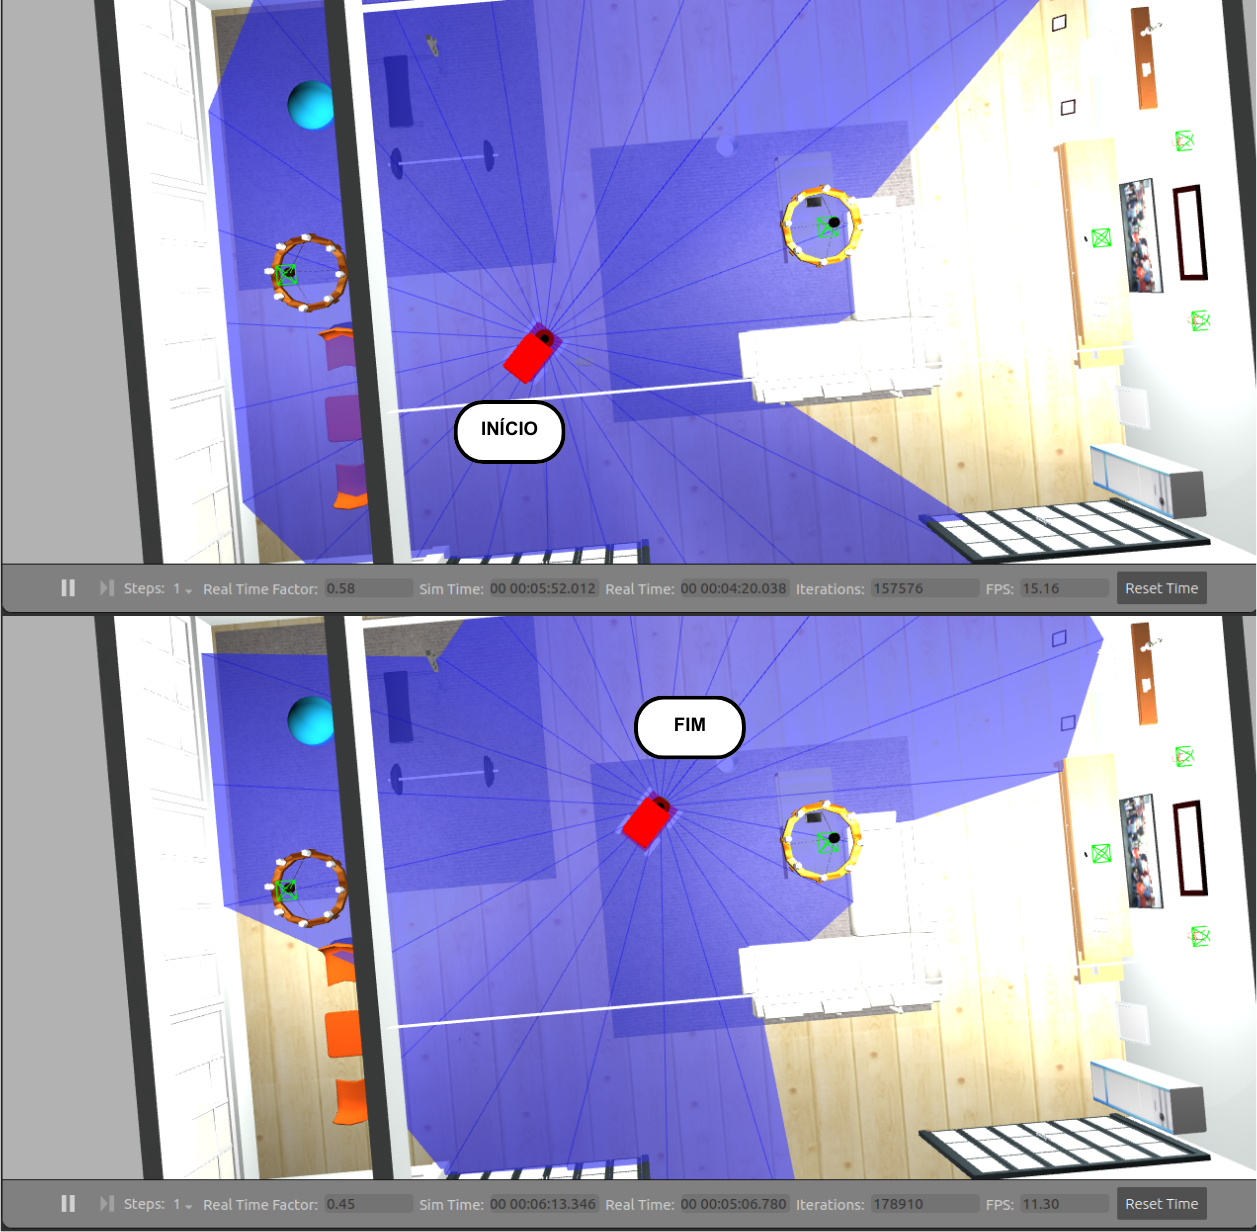
\includegraphics[scale=0.5]{ct03_4.png}
    \caption*{Fonte: Autora (2023).}
    \label{fig:ct03_4}
\end{figure}

\begin{figure}[H]
    \centering
    \caption{Captura da quinta repetição CT03}
    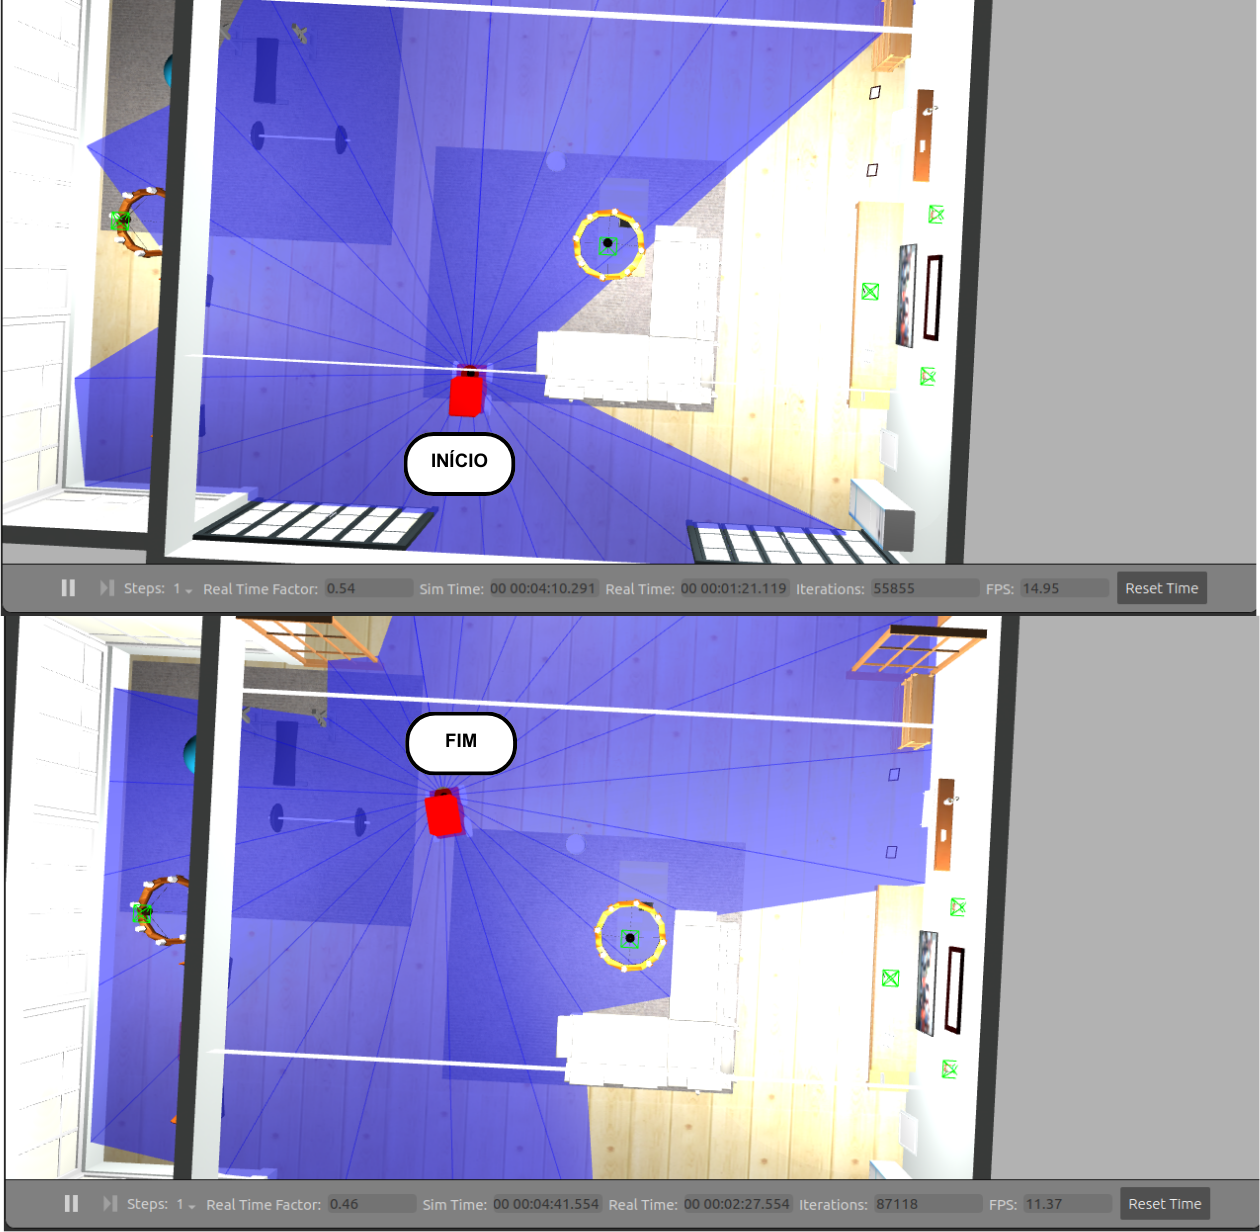
\includegraphics[scale=0.5]{ct03_5.png}
    \caption*{Fonte: Autora (2023).}
    \label{fig:ct03_5}
\end{figure}

\section{Caso de Teste CT04 Referente a RNFS02}
O caso de teste CT04 teve o objetivo de identificar se a velocidade do robô é segura para as pessoas e propriedades ao redor. O caso de teste foi repetido cinco vezes com o robô em lugares distintos no ambiente. Todos os cinco testes foram bem sucedidos. Todos os resultados podem ser visualizados na Tabela~\ref{tab:acertosct04}. Além disso, a seguir podem ser encontradas as capturas para cada repetição (Figura~\ref{fig:ct04_1}, Figura~\ref{fig:ct04_2}, Figura~\ref{fig:ct04_3}, Figura~\ref{fig:ct04_4}, Figura~\ref{fig:ct04_5}).


\begin{table}[H]
\centering
\caption{Resultados das repetições CT04}
\label{tab:acertosct04}
\resizebox{\textwidth}{!}{%
\begin{tabular}{l|c}
                              & \multicolumn{1}{l}{\textbf{Resultados CT04}} \\ \hline
\textbf{Teste 1}              & Bem-sucedido                                 \\
\textbf{Teste 2}              & Bem-sucedido                                 \\
\textbf{Teste 3}              & Bem-sucedido                                 \\
\textbf{Teste 4}              & Bem-sucedido                                 \\
\textbf{Teste 5}              & Bem-sucedido                                 \\
\textbf{Total de acertos (\%)} & \textbf{100}                                  \\ \hline
\end{tabular}%
}
\caption*{Fonte: Autora (2023).}
\end{table}

\begin{figure}[H]
    \centering
    \caption{Captura da primeira repetição CT04}
    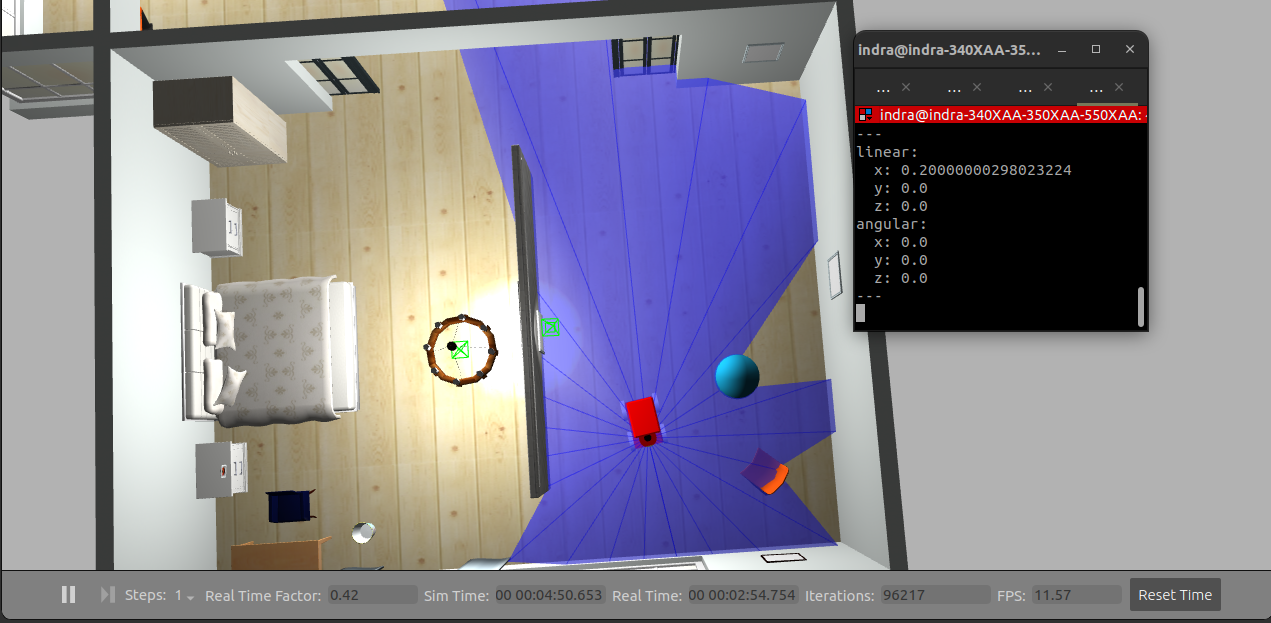
\includegraphics[scale=0.35]{ct04_1.png}
    \caption*{Fonte: Autora (2023).}
    \label{fig:ct04_1}
\end{figure}


\begin{figure}[H]
    \centering
    \caption{Captura da segunda repetição CT04}
    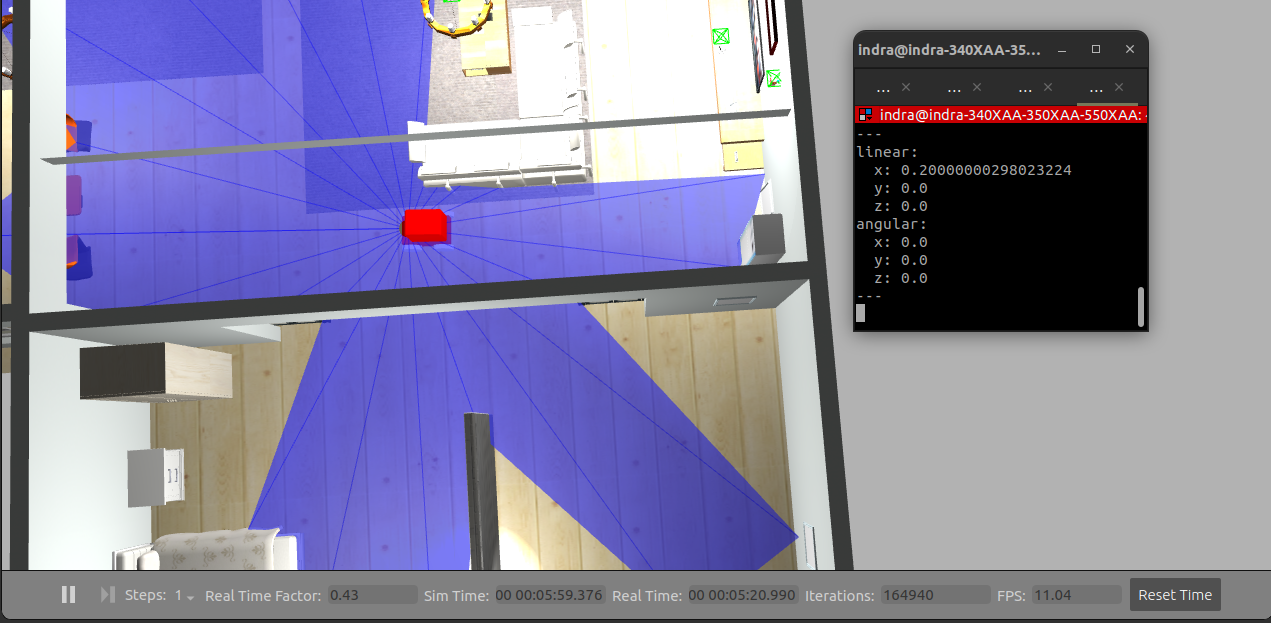
\includegraphics[scale=0.35]{ct04_2.png}
    \caption*{Fonte: Autora (2023).}
    \label{fig:ct04_2}
\end{figure}

\begin{figure}[H]
    \centering
    \caption{Captura da terceira repetição CT04}
    \includegraphics[scale=0.35]{ct04_3.png}
    \caption*{Fonte: Autora (2023).}
    \label{fig:ct04_3}
\end{figure}

\begin{figure}[H]
    \centering
    \caption{Captura da quarta repetição CT04}
    \includegraphics[scale=0.35]{ct04_4.png}
    \caption*{Fonte: Autora (2023).}
    \label{fig:ct04_4}
\end{figure}

\begin{figure}[H]
    \centering
    \caption{Captura da quinta repetição CT04}
    \includegraphics[scale=0.35]{ct04_5.png}
    \caption*{Fonte: Autora (2023).}
    \label{fig:ct04_5}
\end{figure}

\newpage

\section{Caso de Teste CT05 Referente a RNFA01}
O caso de teste CT05 visou validar se o ambiente simulado comportava a mudança de posição dos objetos e móveis ao longo da simulação. O caso de teste foi repetido cinco vezes com o robô em lugares distintos no ambiente. Todos os cinco testes foram bem sucedidos. Todos os resultados podem ser visualizados na Tabela~\ref{tab:acertosct05}. Além disso, a seguir podem ser encontradas as capturas para cada repetição (Figura~\ref{fig:ct05_1}, Figura~\ref{fig:ct05_2}, Figura~\ref{fig:ct05_3}, Figura~\ref{fig:ct05_4}, Figura~\ref{fig:ct05_5}).


\begin{table}[H]
\centering
\caption{Resultados das repetições CT05}
\label{tab:acertosct05}
\resizebox{\textwidth}{!}{%
\begin{tabular}{l|c}
                              & \multicolumn{1}{l}{\textbf{Resultados CT05}} \\ \hline
\textbf{Teste 1}              & Bem-sucedido                                 \\
\textbf{Teste 2}              & Bem-sucedido                                 \\
\textbf{Teste 3}              & Bem-sucedido                                 \\
\textbf{Teste 4}              & Bem-sucedido                                 \\
\textbf{Teste 5}              & Bem-sucedido                                 \\
\textbf{Total de acertos (\%)} & \textbf{100}                                  \\ \hline
\end{tabular}%
}
\caption*{Fonte: Autora (2023).}
\end{table}

\begin{figure}[H]
    \centering
    \caption{Captura da primeira repetição CT05}
    \includegraphics[scale=0.5]{ct05_1.png}
    \caption*{Fonte: Autora (2023).}
    \label{fig:ct05_1}
\end{figure}

\begin{figure}[H]
    \centering
    \caption{Captura da segunda repetição CT04}
    \includegraphics[scale=0.5]{ct05_2.png}
    \caption*{Fonte: Autora (2023).}
    \label{fig:ct05_2}
\end{figure}

\begin{figure}[H]
    \centering
    \caption{Captura da terceira repetição CT04}
    \includegraphics[scale=0.5]{ct05_3.png}
    \caption*{Fonte: Autora (2023).}
    \label{fig:ct05_3}
\end{figure}

\begin{figure}[H]
    \centering
    \caption{Captura da quarta repetição CT04}
    \includegraphics[scale=0.5]{ct05_4.png}
    \caption*{Fonte: Autora (2023).}
    \label{fig:ct05_4}
\end{figure}

\begin{figure}[H]
    \centering
    \caption{Captura da quinta repetição CT04}
    \includegraphics[scale=0.5]{ct05_5.png}
    \caption*{Fonte: Autora (2023).}
    \label{fig:ct05_5}
\end{figure}

\section{Caso de Teste CT06 Referente a RNFA03}
O caso de teste CT06 teve o objetivo de identificar se a simulação apresenta um ambiente semelhante a um domicílio comum. Na Figura~\ref{fig:ct06}, pode ser encontrada a captura do teste.

\begin{figure}[H]
    \centering
    \caption{Captura do teste CT06}
    \includegraphics[scale=0.35]{ct06.png}
    \caption*{Fonte: Autora (2023).}
    \label{fig:ct06}
\end{figure}

\section{Caso de Teste CT07 Referente a RNFA04}
O caso de teste CT07 teve o objetivo de identificar o tamanho do domicílio apresentado na simulação. Na Figura~\ref{fig:ct07}, pode ser encontrada a captura do teste.

\begin{figure}[H]
    \centering
    \caption{Captura do teste CT07}
    \includegraphics[scale=0.45]{ct07.png}
    \caption*{Fonte: Autora (2023).}
    \label{fig:ct07}
\end{figure}

\section{Caso de Teste CT08 Referente a RNFA05}
O caso de teste CT08 visou identificar o acesso entre os espaços do ambiente simulado. Na Figura~\ref{fig:ct08}, pode ser encontrada a captura do teste.

\begin{figure}[H]
    \centering
    \caption{Captura do teste CT08}
    \includegraphics[scale=0.5]{ct08.png}
    \caption*{Fonte: Autora (2023).}
    \label{fig:ct08}
\end{figure}



\annex


%
% Finalização do documento. A partir desse comando qualquer coisa escrita será ignorada:
%

\end{document}
